%\newsection{Kapitel1}

%Hier den Inhalt mit \input einfügen und die folgenden Zeilen entfernen

%\include{nomenclature.tex}
%Lernziele 1
\begin{frame}
    \b{
        \begin{Lernziele}{Operationsverstärker}
            \title{Lernziele: Operationsverstärker}
            Die Studierenden können
            \begin{itemize}
                \item den Aufbau eines einfachen Operationsverstärkers angeben.
                \item das Funktionsprinzip eines Operationalverstärkers erläutern.
                \item verschiedene Operationsverstärkerschaltungen und mögliche Einsatzgebiete nennen. 
                \item Unterschiede zwischen dem vereinfachten Operationsverstärkermodell und realen Operationsverstärkern beschreiben und wichtige Bereiche der Operationsverstärkerkennlinie angeben.
                \item die Funktion von vorliegenden Operationsverstärkerschaltungen bestimmen und mithilfe der Kirchhoff'schen Gesetze die Verstärkung berechnen.
            \end{itemize}
        \end{Lernziele}    
    }

   % \speech{Lernziele}{1}{
    %    Lernziele des Kapitels Operationsverstärker:
     %   Die studierenden können den Aufbau eines einfachen Operationsverstärkers angeben, das Funktionsprinzip eines Operationalverstärkers erläutern, 
      %  verschiedene Operationsverstärkerschaltungen und mögliche Einsatzgebiete nennen, Unterschiede zwischen dem vereinfachten Operationsverstärkermodell und realen Operationsverstärkern beschreiben und wichtige Bereiche der Operationsverstärkerkennlinie angeben, die Funktion von vorliegenden Operationsverstärkerschaltungen bestimmen und mithilfe der Kirchhoff'schen Gesetze die Verstärkung berechnen.
    %}




    
\end{frame}

%Lernziele 2
\begin{frame}
\b{
    \begin{Lernziele}{Operationsverstärker}
        \title{Lernziele: Operationsverstärker}
        Die Studierenden können
        \begin{itemize}
            \item geeignete Operationsverstärkerschaltungen für eine Problemlösung angegeben, Widerstandsverhältnisse berechnen und die Schaltung aufzeichnen.
            \item wichtige Eigenschaften von Operationsverstärkerschaltungen benennen.
            \item Stabilitätsanalysen durchführen und Ergebnisse der Analyse beurteilen.
            \item auf Grundlage von Datenblättern Vor- und Nachteile von Operationsverstärkern für bestimmte Einsatzzwecke benennen und geeignete Komponenten für vorliegende Problemstellungen auswählen.
        \end{itemize}
    \end{Lernziele}    
}
\end{frame}

% \speech{Lernziele}{1}{
    %    Lernziele des Kapitels Operationsverstärker:
     %   Die studierenden können geeignete Operationsverstärkerschaltungen für eine Problemlösung angeben, Widerstandsverhältnisse berechnen und die Schaltung aufzeichnen, wichtige Eigenschaften von Operationsverstärkerschaltungen benennen, Stabilitätsanalysen durchführen und Ergebnisse der Analyse beurteilen, auf Grundlage von Datenblättern Vor- und Nachteile von Operationsverstärkern für bestimmte Einsatzzwecke benennen und geeignete Komponenten für vorliegende Problemstellungen auswählen.
    %}



%Einführungsfolie
\begin{frame}
    %\listoftodos
    %Skript
    \fta{Einführung, Aufbau und Funktionsweise von Operationsverstärkern}
    \ftx{Einführung}
    \s{Im vorherigen Modul wurde erläutert, wie mit Hilfe von ein- und mehrstufigen Transistorverstärkern,
    Signale mit geringen Eingangsamplituden verstärkt werden können. Diese Verstärkerschaltungen wurden 
    vor allem in der Mess-, Steuer- und Regelungstechnik eingesetzt und bis in die 1950er Jahre diskret 
    aus Elektronenröhren oder Transistoren aufgebaut. Die Entwicklung der „integrated curcuits“ ermöglichte 
    ab Ende der 1960er Jahre die Miniaturisierung von Schaltungen und dadurch die Bereitstellung 
    von modularen Bausteinen für die Hardwareentwicklung. Dies galt auch für die in den 1940er Jahren entwickelte 
    Differenzverstärker, die aufgrund ihres zunächst sehr verbreiteten Einsatzes in Analogrechnern auch als 
    „operational amplifier“ (zu deutsch „Operationsverstärker“ von „Operator“) bezeichnet werden. 
    Die Grundlagen zum Thema „Operationsverstärker“ werden in diesem Modul vermittelt. 

    Es sollen im Rahmen dieses Kapitels folgende Kompetenzen erworben werden:


    % \speech{Einführung Operationsverstärker}{1}{
    %   Im vorherigen Modul wurde erläutert, wie mit Hilfe von ein- und mehrstufigen Transistorverstärkern,
    %   Signale mit geringen Eingangsamplituden verstärkt werden können. Diese Verstärkerschaltungen wurden 
    %   vor allem in der Mess-, Steuer- und Regelungstechnik eingesetzt und bis in die 1950er Jahre diskret 
    %   aus Elektronenröhren oder Transistoren aufgebaut. Die Entwicklung der „integrated circuits“ ermöglichte 
    %    ab Ende der 1960er Jahre die Miniaturisierung von Schaltungen und dadurch die Bereitstellung 
    %    von modularen Bausteinen für die Hardwareentwicklung. Dies galt auch für die in den 1940er Jahren entwickelte 
    %    Differenzverstärker, die aufgrund ihres zunächst sehr verbreiteten Einsatzes in Analogrechnern auch als 
    %    „operational amplifier“ (zu deutsch „Operationsverstärker“ von „Operator“) bezeichnet werden. 
    %    Die Grundlagen zum Thema „Operationsverstärker“ werden in diesem Modul vermittelt. 

    %    Es sollen im Rahmen dieses Kapitels folgende Kompetenzen erworben werden:
 %   }



    \s{
        \begin{Lernziele}{Operationsverstärker}
            \title{Lernziele: Operationsverstärker}
            Die Studierenden können
            \begin{itemize}
                \item den Aufbau eines einfachen Operationsverstärkers angeben.
                \item das Funktionsprinzip eines Operationsverstärkers erläutern.
            \end{itemize}
        \end{Lernziele}
    }

    %\speech{Einführung Operationsverstärker}{1}{
    %Die Studierenden können den Aufbau eines einfachen Operationsverstärkers angeben und das Funktionsprinzip eines Operationsverstärkers erläutern. 
    %}



    \ftb{Aufbau und Funktionsweise}
    Operationsverstärker (auch kurz als OPV oder OpAmp bezeichnet) zeichnen sich dadurch aus, 
    dass sie als Universalverstärker aufgebaut sind und ihre Funktion maßgeblich durch äußere Beschaltung bestimmt 
    wird. So lassen sich mit dem gleichen Baustein Spannungen  verstärken, Rechenoperationen wie Additionen, Subtraktionen 
    oder Integrationen durchführen und Signale schalten. Solche Operationalverstärker sind beispielsweise in der Mess- und 
    Regelungstechnik, der Signalverarbeitung und der Signalformung unerlässlich. Im Folgenden ist ein aus diskreten 
    Transistoren aufgebauter Operationsverstärker und ein integrierter Schaltkreis dargestellt.
	Durch die direkte Kopplung der Verstärkerstufen können Operationsverstärker
    Gleich- und Wechselspannungen verstärken und werden aus diesem Grund der Gruppe 
    der Gleichspannungsverstärker zugeordnet. 

    %\speech{Einführung Operationsverstärker}{1}{
    %Operationsverstärker (auch kurz als OPV oder OpAmp bezeichnet) zeichnen sich dadurch aus, dass sie als Universalverstärker aufgebaut sind und ihre Funktion maßgeblich durch äußere Beschaltung bestimmt wird. So lassen sich mit dem gleichen Baustein Spannungen  verstärken, Rechenoperationen wie Additionen, Subtraktionen oder Integrationen durchführen und Signale schalten. Solche Operationalverstärker sind beispielsweise in der Mess- und Regelungstechnik, der Signalverarbeitung und der Signalformung unerlässlich. Im Folgenden ist ein aus diskreten Transistoren aufgebauter Operationsverstärker und ein integrierter Schaltkreis dargestellt. 
    %Durch die direkte Kopplung der Verstärkerstufen können Operationsverstärker Gleich- und Wechselspannungen verstärken und werden aus diesem Grund der Gruppe der Gleichspannungsverstärker zugeordnet.
    %}

    %Abbildungen DIP Package OPV und Diskret Skript
    \begin{minipage}[t]{0.5\textwidth}
        \f{width=0.6\textwidth}{width=0.8\textwidth}{kap1/OpAmpDiskret.png}{Diskret aufgebauter Operationsverstärker {\tiny(Quelle: Analog Devices, Wikipedia, Lizenz CC-BY-SA)}} % https://de.wikipedia.org/wiki/Operationsverst%C3%A4rker#/media/Datei:Discrete_opamp.png
    \end{minipage}    
    \begin{minipage}[t]{0.5\textwidth}
        \f{width=0.67\textwidth}{width=0.8\textwidth}{kap1/OpAmpPackage.png}{Operationsverstärker monolithisch in Dual in-line package (DIP) {\tiny(Quelle: Wollschaf, Wikipedia, (GNU-Lizenz für freie Dokumentation – mit Namensnennung))}} % https://de.wikipedia.org/wiki/Datei:Integrated_Circuit.jpg
    \end{minipage}  
%    \speech{
%       Abbildung 1.1 zeigt einen diskret aufgebauten Operationsverstärker. Die Darstellung ist in Schwarz-Weiß gehalten und gibt einen detaillierten Einblick in die interne Struktur der elektronischen Bauteile. Mehrere kleine zylindrische Bauteile, wahrscheinlich Kondensatoren, sind sichtbar, zusammen mit einer Vielzahl von Widerständen und anderen diskreten Komponenten, die auf einer Leiterplatte angeordnet sind. In der unteren Hälfte sind zwei herausragende Metallpins erkennbar, die zur externen Verbindung dienen. Das gesamte Bild hat eine leicht körnige Struktur, die auf eine makroskopische Aufnahme hinweist.
%        
%        Abbildung 1.2 zeigt einen monolithischen Operationsverstärker in einem Dual-Inline-Package (DIP). Dieses Bauteil ist ein integrierter Schaltkreis, der in einem rechteckigen schwarzen Kunststoffgehäuse untergebracht ist. Auf der Oberseite ist eine Beschriftung zu sehen, die vermutlich die Typenbezeichnung und den Hersteller angibt. Das Gehäuse ist auf beiden Längsseiten mit insgesamt 14 Metallpins ausgestattet, die leicht nach außen gebogen sind und der elektrischen Verbindung dienen. Der Schattenwurf auf der weißen Oberfläche zeigt, dass die Pins leicht schräg vom Bauteil abstehen.
%        }
        
    }

    %Abbildungen DIP Package OPV und Diskret Beamer
    \b{\begin{columns}
            \column[c]{0.3\textwidth}
                \f{width=0.4\textwidth}{width=0.8\textwidth}{kap1/OpAmpDiskret.png}{Diskret aufgebauter Operationsverstärker {\tiny(Quelle: Analog Devices, Wikipedia, Lizenz CC-BY-SA)}} % https://de.wikipedia.org/wiki/Operationsverst%C3%A4rker#/media/Datei:Discrete_opamp.png
                \f{width=0.4\textwidth}{width=0.8\textwidth}{kap1/OpAmpPackage.png}{Operationsverstärker monolithisch in Dual in-line package (DIP) {\tiny(Quelle: Wollschaf, Wikipedia, (GNU-Lizenz für freie Dokumentation – mit Namensnennung))}} % https://de.wikipedia.org/wiki/Datei:Integrated_Circuit.jpg
                \column[c]{0.6\textwidth}
                %Beamer
                \frametitle{Historie und Aufbau}
                    \begin{itemize}
                    \onslide<1->{
                    \item Mehrstufige Transistorverstärker können genutzt werden, um Signale zu verstärken (siehe Kap. Halbleiter).}
                    \onslide<2->{
                    \item Nach diesem Prinzip entworfene Schaltungen wurden bis zur Entwicklung der integrierten Schaltkreise (IC) diskret als Universalverstärker aufgebaut.}
                    \onslide<3->{
                    \item Heute werden Universalverstärker monolithisch aufgebaut. Ihr Verhalten für den gewünschten Einsatzzweck wird maßgeblich durch die äußere Beschaltung bestimmt.}
                    \onslide<4->{
                    \item Sie werden in der Regel aufgrund ihres ursprünglichen Einsatzes in Analogrechnern als \glqq Operationsverstärker\grqq{} bezeichnet.}
                \end{itemize}
            \end{columns}}
    
    %Gesprochener Text 
    %\speech{Einführung Operationsverstärker}{1}{Im letzten Kapitel haben wir besprochen, wie man Signale mit kleinen Eingangsamplituden durch ein- und mehrstufige Transistorverstärker verstärken kann. Diese Verstärkerschaltungen wurden vor allem in der Mess-, Steuer- und Regelungstechnik verwendet und bis in die 1950er Jahre aus diskreten Elektronenröhren oder Transistoren aufgebaut. Mit der Entwicklung der integrierten Schaltungen in den späten 1960er Jahren wurde die Fertigung und Miniaturisierung von Schaltungen möglich, was wiederum die Bereitstellung von modularen Bausteinen für die Hardwareentwicklung ermöglichte.
    %Das gilt auch für die in den 1940er Jahren entwickelten Differenzverstärker, die aufgrund ihres weit verbreiteten Einsatzes in Analogrechnern auch als Operationsverstärker bezeichnet werden. Diese Verstärker sind als Universalverstärker konzipiert und ihre Funktion wird nur durch die äußere Beschaltung bestimmt. Mit dem gleichen Baustein kann man also Spannungen verstärken, Rechenoperationen wie Addition, Subtraktion oder Integration durchführen und Signale schalten. Operationsverstärker sind in der Mess- und Regeltechnik, der Signalverarbeitung und der Signalformung unerlässlich.
    %Im Folgenden wird ein Operationsverstärker gezeigt, der aus diskreten Transistoren aufgebaut ist, sowie ein integrierter Schaltkreis. Durch die direkte Kopplung der Verstärkerstufen können Operationsverstärker sowohl Gleich- als auch Wechselspannungen verstärken und gehören deshalb zur Gruppe der Gleichspannungsverstärker.}
\end{frame}

\begin{frame}
    \b{
    \frametitle{Komparator}
    \begin{figure}[H]
    \centering
    % Linkes Bild
    \begin{subfigure}[b]{\textwidth}
        \centering
        \begin{tikzpicture}
\ctikzset{tripoles/en amp/input height=0.45}
\draw (0,0)node[en amp](E){}
    (E.out)
    (E.-)
    (E.+);
    \draw (E.out)  to[short, -o] (2.5,0);
    
    \draw (E.-)  to[short, -o] (-6,0.5);

    \draw (E.+) to[short, -o] (-3,-0.5);
    \draw (-3,-2)node[ground]{};

    \draw (-6,-2) to[short, o-o] (-3,-2) to[short,-o] ( 2.5,-2);

    \draw (2.5,0) to [open, v>,name=U0] (2.5,-2);
    
    \draw (-6,0.5) to [open, v>,name=UE] (-6,-2);
    
    \draw (-3,-0.5) to [open, v>,name=UREF] (-3,-2);

    

\varrmore {U0}{$U_\mathrm{A}$};
\varrmore {UE}{$U_\mathrm{E}$};
\varrmore {UREF}{$U_\mathrm{Ref}$};

\end{tikzpicture}
    \end{subfigure}

    \begin{subfigure}[b]{\textwidth}
        \centering
        \includesvg[width=0.6\textwidth]{Bilder/Aufgaben/FigAkkuUeberwachung}
    \end{subfigure}
    \label{fig:Komparator}
    \end{figure}
    }
\end{frame}

\begin{frame}
   \b{
    \frametitle{Funktionsweise von Operationsverstärkern}
    Die Funktionsweise lässt sich gut an folgender Schaltung nachvollziehen. Was passiert, wenn an dieser Schaltung eine positve Differenzspannung angelegt wird?
    \begin{figure}[ht]
        \centering
        \fu{
            \resizebox{0.7\textwidth}{!}{\begin{circuitikz}
    \ctikzset{
        transistors/scale=1.3,
        resistors/scale=0.4,
        diodes/scale=0.5,
    }
    \draw (1,0) node[npn] (T1) {}
          (6,1) node[pnp, yscale=1] (T2) {}
          (2,-2) node[npn, xscale=-1] (T3) {}
          (3,0) node[npn, xscale=-1] (T4) {};
    \draw (T1.B) -- (-1,0) node[ocirc, label=north:{$-$}] {}; 
    \draw (T1.C) to[R] ++(0,1) -| (7,2) node[ocirc, label=right:{$+U_B$}] {};
    \draw (T1.E)  |- (T4.E);
    \draw (T2.C) -- ++(0,-1) to[R, l= \textit{R}$_L$] ++(0,-3) node[circ]{};
    \draw (T2.B)  |- (T4.C);
    \draw (T3.C) -- ++(0,0) node[circ] {};
    \draw (T3.E) to[R] ++(0, -0.5) -- ++(0,-0.5) -| (7,-4) node[ocirc, label=right:{$-U_B$}] {};
    \draw (T3.B) -- ++(1.5,0) to[R] ++(0, 4) node[circ] {};
    \draw (T3.B) node[circ] {} to[D, l=\textit{D}$_1$] ++(0,-1) to[D, l=\textit{D}$_2$] ++(0,-1) node[circ] {};
    \draw (T2.E) -- ++(0,0) node[circ] {};
    \draw (T4.C) node[circ]{} -- ++(0,0) to[R] ++(0,1) node[circ]{};
    \draw (T4.B) -- ++(0,-1.5) -- (-1,-1.5) node[ocirc, label=north:{$+$}] {};
    \draw (T2.C) -- ++(0,-1) node[circ]{} -- ++(0.5,0) node[ocirc, label=right:{$U_A$}] {};

 
 \node at (0.5, 0.6) {\textit{T}$_1$};
 \node at (3.8, 0.2) {\textit{T}$_2$};
 \node at (2.8, -1.8) {\textit{T}$_3$};
 \node at (5.2, 1.2) {\textit{T}$_4$};
\end{circuitikz}}
            }{Verhalten eines vereinfachten Operationsverstärkers bei Anlegen einer positiven Differenzspannung am Eingang 
            \label{fig:Funktionsweise OPV Folien ohne Pfeile}}
    \end{figure}
   } 
\end{frame}

%\speech{
%Abbildung 1.3 zeigt das Verhalten eines vereinfachten Operationsverstärkers, wenn eine positive Differenzspannung am Eingang anliegt.  
%Die Schaltung ist in drei farblich hervorgehobene Bereiche unterteilt.  
%Ein roter Bereich links, ein violetter Bereich unten und ein gelber Bereich rechts.  
%Blaue Pfeile zeigen, wie sich das elektrische Potenzial an verschiedenen Punkten der Schaltung verändert.  
%
%Der rote Bereich stellt eine Differenzverstärkerstufe dar.  
%Diese besteht aus zwei Transistoren, die die Differenzspannung am Eingang verarbeiten.  
%Der positive Eingang erhält eine höhere Spannung als der negative Eingang, wodurch sich der Stromfluss in den Transistoren ändert.  
%
%Der violette Bereich enthält zwei Dioden.  
%Diese Dioden stabilisieren das Spannungsverhalten zwischen den Transistoren und den nachfolgenden Verstärkerstufen.  
%
%Der gelbe Bereich zeigt die Ausgangsstufe des Operationsverstärkers.  
%Die Versorgungsspannung ist durch Plus U B und Minus U B gekennzeichnet.  
%Ein Lastwiderstand ist zwischen dem Ausgang und der negativen Versorgungsspannung geschaltet.  
%Die Spannung U A stellt die Ausgangsspannung dar, die sich entsprechend der Eingangsdifferenzspannung verändert.  
%
%Die Abbildung zeigt, wie eine kleine Änderung der Eingangsspannung eine größere Änderung der Ausgangsspannung bewirkt.  
%}

%\speech {Funktionsweise von Operationsverstärkern}{1}{
 %   Die Funktionsweise lässt sich gut an einem vereinfachten Ersatzschaltbild erklären. 
 %In dieser Abbildung ist ein vereinfachtes Ersatzschaltbild eines OPVs aus Bipolartransistoren dargestellt. 
 %Heute werden Operationsverstärker vermehrt aus Feldeffekttransistoren (FET) aufgebaut. 
 %Die Umsetzung der Verstärkerschaltungen mit FETs erfolgt aber sehr ähnlich zu Bipolartransistoren, 
 %weswegen die Funktionsweise hier mit einer Art von Transistoren gezeigt werden soll. 
 %Die NPN-Transistoren $T_1$ und $T_2$ sind identisch und bilden den Eingang des Operationsverstärkers. 
 %Zwischen dem mit „+“ gekennzeichneten Eingang und dem mit „-“ gekennzeichneten Eingang 
 %wird die zu verstärkende Differenzspannung $U_{\textnormal{Diff}}$ angelegt. Die Eingänge werden als nicht-invertierender Eingang 
 %„+“ und invertierender Eingang „-“ bezeichnet. Dieser Differenzverstärker am Eingang des OPVs ist in der unteren Abbildung rot umrandet. 
 %Der Transistor $T_3$ funktioniert durch die Verschaltung mit den Dioden $D_1$ und $D_2$ wie eine Konstantspannungsquelle bzw. Strombegrenzung. 
 %Die zwei Dioden sorgen für eine Regulierung der Basisspannung an $T_3$. Dieser Teil der Schaltung ist lila markiert. 
 %Wenn die nicht-invertierte Eingangsspannung steigt, sinkt der Widerstand des Transistors $T_2$. 
 %Das führt zu einer Reduktion der Spannung am Kollektor von $T_2$ und einem Anstieg am Emitter. 
 %Da die Basis des Transistors $T_4$ mit dem Kollektor von $T_2$ verbunden ist, 
 %verursacht dies eine entsprechende Spannungsreduktion an der Basis von $T_4$. 
 %Infolgedessen wird der Kollektor-Emitter-Pfad des PNP-Transistors $T_4$ hochohmiger, 
 %so dass mehr Strom durch den Lastwiderstand $R_{\textnormal{L}}$ fließt. 
 %Dadurch erhöht sich der Spannungsabfall über $R_{\textnormal{L}}$ und somit die Spannung am Ausgang $U_{\textnormal{A}}$.} 


\begin{frame}
    \s{Die Funktionsweise lässt sich gut an einem vereinfachten Ersatzschaltbild erklären (siehe Abbildung~\ref{fig:Funktionsweise OPV 1}). 
    In dieser Abbildung ist ein vereinfachtes Ersatzschaltbild eines OPVs aus Bipolartransistoren dargestellt. 
    Heute werden Operationsverstärker vermehrt aus Feldeffekttransistoren (FET) aufgebaut. 
    Die Umsetzung der Verstärkerschaltungen mit FETs erfolgt aber sehr ähnlich zu Bipolartransistoren, weswegen die Funktionsweise hier mit einer Art von Transistoren gezeigt werden soll. 
    Die NPN-Transistoren $T_1$ und $T_2$ sind identisch und bilden den Eingang des Operationsverstärkers. Zwischen dem mit „+“ gekennzeichneten Eingang und dem mit „-“ gekennzeichneten Eingang wird die zu verstärkende Differenzspannung $U_{\textnormal{Diff}}$ angelegt\footnote{Alle in diesem Modul vorkommenden Ströme und Spannungen können zeitlich veränderlich sein und werden im Folgenden nur aufgrund der Übersichtlichkeit nicht mit $U_{\textnormal{E/A/...}}(t)$ sondern mit $U_{\textnormal{E/A/...}}$ bezeichnet}. 
    Die Eingänge werden als nicht-invertierender Eingang „+“ und invertierender Eingang „-“ bezeichnet. 
    Dieser Differenzverstärker am Eingang des OPVs ist in Abbildung~\ref{fig:Funktionsweise OPV 1} rot umrandet. 
    Der Transistor $T_3$ funktioniert durch die Verschaltung mit den Dioden $D_1$ und $D_2$ wie 
    eine Stromquelle. Die zwei Dioden sorgen für eine Regulierung der Basis-Spannung an $T_3$ (dieser Teil der Schaltung ist lila markiert).
    
    Wenn die nicht-invertierte Eingangsspannung steigt (A), sinkt der Widerstand des Transistors $T_2$. 
    Dies führt zu einer Reduktion der Spannung an dessen Kollektor und zu einem Anstieg am Emitter~(B). Da die Basis des Transistors $T_4$ mit dem Kollektor von $T_2$ verbunden ist, verursacht dies einen entsprechende Spannungsreduktion an der Basis von $T_4$ (C). 
    Infolgedessen wird der Kollektor-Emitter-Pfad des PNP-Transistors $T_4$ hochohmiger, so dass mehr Strom durch den Lastwiderstand $R_{\textnormal{L}}$ fließt~(D). 
    Dadurch erhöht sich der Spannungsabfall über $R_{\textnormal{L}}$ und somit die Spannung am Ausgang $U_{\textnormal{A}}$ (die Ausgangsstufe des Verstärkers ist gelb markiert).
    
    %Figure 1.3 im Skript
    \begin{minipage}{\textwidth}        
        \centering
        \fu{
            \resizebox{0.6\textwidth}{!}{\begin{circuitikz}
    \ctikzset{
        transistors/scale=1.3,
        resistors/scale=0.4,
        diodes/scale=0.5,
    }
    \fill[red, opacity=0.2] (4.3,-1.5) rectangle (-1.6,2.2);
    \fill[yellow, opacity=0.2] (8,-4.2) rectangle (4.9,2.2);
    \fill[violet, opacity=0.2] (4,-4.2) rectangle (1.5,-1.5);

    \draw (1,0) node[npn] (T1) {}
          (6,1) node[pnp, yscale=1] (T2) {}
          (2,-2) node[npn, xscale=-1] (T3) {}
          (3,0) node[npn, xscale=-1] (T4) {};
    \draw (T1.B) -- (-1,0) node[ocirc, label=north:{$-$}] {}; 
    \draw (T1.C) to[R] ++(0,1) -| (7,2) node[ocirc, label=right:{{$+U_{\textnormal{B}}$}}] {};
    \draw (T1.E)  |- (T4.E);
    \draw (T2.C) -- ++(0,-1) to[R, l= \textit{R}$_{\textnormal{L}}$] ++(0,-3) node[circ]{};
    \draw (T2.B)  |- (T4.C);
    \draw (T3.C) -- ++(0,0) node[circ] {};
    \draw (T3.E) to[R] ++(0, -0.5) -- ++(0,-0.5) -| (7,-4) node[ocirc, label=right:{$-U_{\textnormal{B}}$}] {};
    \draw (T3.B) -- ++(1.5,0) to[R] ++(0, 4) node[circ] {};
    \draw (T3.B) node[circ] {} to[D, l=\textit{D}$_1$] ++(0,-1) to[D, l=\textit{D}$_2$] ++(0,-1) node[circ] {};
    \draw (T2.E) -- ++(0,0) node[circ] {};
    \draw (T4.C) node[circ]{} -- ++(0,0) to[R] ++(0,1) node[circ]{};
    \draw (T4.B) -- ++(0,-1.3) -- (-1,-1.3) node[ocirc, label=north:{$+$}] {};
    \draw (T2.C) -- ++(0,-1) node[circ]{} -- ++(0.5,0) node[ocirc, label=right:{$U_{\textnormal{A}}$}] {};
    
    \draw[red, thick] (4.3,-1.5) rectangle (-1.6,2.2);
    \draw[yellow, thick] (8,-4.2) rectangle (4.9,2.2);
    \draw[violet, thick] (4,-4.2) rectangle (1.5,-1.5);


\draw[-{Triangle[width=3pt,length=4pt]}, color=spannung] (5.3,0.3) -- (5.3,0.9) node[midway, right] {};
 \draw[-{Triangle[width=3pt,length=4pt]}, color=spannung] (7.3,0) -- (7.3,-2) node[midway, right] {};
 \draw[-{Triangle[width=3pt,length=4pt]}, color=spannung] (2,-0.9) -- (2,-0.3) node[midway, right] {};
 \draw[-{Triangle[width=3pt,length=4pt]}, color=spannung] (2.8,0.6) -- (2.8,1.2) node[midway, right] {};
 \draw[-{Triangle[width=3pt,length=4pt]}, color=spannung] (1.2,1) -- (1.2,0.4) node[midway, left] {};
 \draw[-{Triangle[width=3pt,length=4pt]}, color=spannung]  (-0.7, -0.2) -- (-0.7, -1.1) node[midway, right] {$U_{\text{Diff}}$};

\end{circuitikz}}
            } 
            {Verhalten eines vereinfachten Operationsverstärkers bei Anlegen einer positiven Differenzspannung am Eingang. Die blauen Pfeile geben an, wie sich das Potential am Schaltungsknoten ggü. eines ausgeglichenen Eingangs $U_{\textnormal{Diff}}$~=~0 verschiebt.
            \label{fig:Funktionsweise OPV 1}}
    \end{minipage}
    }
    
    \b{ %Figure 1.3 auf Folien
        \frametitle{Funktionsweise von Operationsverstärkern}
        \begin{figure}[ht]
                \centering
                \fu{
                \resizebox{0.7\textwidth}{!}{
    \begin{circuitikz}[scale=1, transform shape]
        \ctikzset{
            transistors/scale=1.3,
            resistors/scale=0.4,
            diodes/scale=0.5,
        }
        \draw (1,0) node[npn] (T1) {}
              (6,1) node[pnp, yscale=1] (T2) {}
              (2,-2) node[npn, xscale=-1] (T3) {}
              (3,0) node[npn, xscale=-1] (T4) {};
        \draw (T1.B) -- (-1,0) node[ocirc, label=north:{$-$}] {}; 
        \draw (T1.C) to[R] ++(0,1) -| (7,2) node[ocirc, label=right:{{$+U_{\textnormal{B}}$}}] {};
        \draw (T1.E)  |- (T4.E);
        \draw (T2.C) -- ++(0,-1) to[R, l= \textit{R}$_{\textnormal{L}}$] ++(0,-3) node[circ]{};
        \draw (T2.B)  |- (T4.C);
        \draw (T3.C) -- ++(0,0) node[circ] {};
        \draw (T3.E) to[R] ++(0, -0.5) -- ++(0,-0.5) -| (7,-4) node[ocirc, label=right:{$-U_{\textnormal{B}}$}] {};
        \draw (T3.B) -- ++(1.5,0) to[R] ++(0, 4) node[circ] {};
        \draw (T3.B) to[D, l=\textit{D}$_1$] ++(0,-1) to[D, l=\textit{D}$_2$] ++(0,-1) node[circ] {};
        \draw (T2.E) -- ++(0,0) node[circ] {};
        \draw (T4.C) node[circ]{} -- ++(0,0) to[R] ++(0,1) node[circ]{};
        \draw (T4.B) -- ++(0,-1.3) -- (-1,-1.3) node[ocirc, label=north:{$+$}] {};
        \draw (T2.C) -- ++(0,-1) node[circ]{} -- ++(0.5,0) node[ocirc, label=right:{$U_{\textnormal{A}}$}] {};
        
        \node at (-1,-0.5) {\textbf{\LARGE A}};
        \node at (2.2,1)  {\textbf{\LARGE B}};
        \node at (0.5, 0.6) {\textit{T}$_1$};
        \node at (3.8, 0.2) {\textit{T}$_2$};
        \node at (2.8, -1.8) {\textit{T}$_3$};
        \node at (5.2, 1.2) {\textit{T}$_4$};

        \draw[-{Triangle[width=3pt,length=4pt]}, color=spannung] (2.8,1.2) -- (2.8,0.6) node[midway, right] {};
        \draw[-{Triangle[width=3pt,length=4pt]}, color=spannung] (2,-0.9) -- (2,-0.3) node[midway, right] {};
        \draw[-{Triangle[width=3pt,length=4pt]}, color=spannung] (5.3,0.9) -- (5.3,0.3) node[midway, right] {};
        \draw[-{Triangle[width=3pt,length=4pt]}, color=spannung] (-0.7, -1.1) -- (-0.7, -0.2) node[midway, right] {$U_{\text{Diff}}$};


    \end{circuitikz} 
}
                }{Verhalten eines vereinfachten Operationsverstärkers bei Anlegen einer positiven Differenzspannung am Eingang.
                \label{fig:Funktionsweise OPV 1 Folien Teil 1}}
        \end{figure}   
        Eine positive Differenzspannung (A) führt zu einer Reduktion des Widerstands von $T_2$, was zu einer Spannungsreduktion an dessen Kollektor und einem Anstieg am Emitter führt (B). $T_3$ fungiert als Stromquelle.}
    %\speech{Funktionsweise von Operationsverstärkern Folie 1}{1}{
    % Die Funktionsweise von Operationsverstärkern lässt sich gut an einem vereinfachten Ersatzschaltbild erklären. 
    %Die NPN-Transistoren T1 und T2 sind identisch und bilden den Eingang des Operationsverstärkers. 
    %Zwischen dem mit „+“ gekennzeichneten Eingang und dem mit „-“ gekennzeichneten Eingang wird die zu verstärkende Differenzspannung angelegt. 
    %Die Eingänge werden als nicht-invertierender Eingang „+“ und invertierender Eingang „-“ bezeichnet. 
    % Dieser Differenzverstärker ist in der unteren Abbildung rot umrandet. 
    %Der Transistor T3 funktioniert durch die Verschaltung mit den Dioden D1 und D2 wie eine Konstantspannungsquelle bzw. Strombegrenzung. 
    %Die zwei Dioden sorgen für eine Regulierung der Basisspannung an T3. Dieser Teil der Schaltung ist lila markiert.
    %}

\end{frame}

\begin{frame}\b{
    \frametitle{Funktionsweise von Operationsverstärkern}
    \begin{figure}[ht]
            \centering
            \fu{
            \resizebox{0.7\textwidth}{!}{    \begin{circuitikz}[scale=1, transform shape]
        \ctikzset{
            transistors/scale=1.3,
            resistors/scale=0.4,
            diodes/scale=0.5,
        }
        \draw (1,0) node[npn] (T1) {}
              (6,1) node[pnp, yscale=1] (T2) {}
              (2,-2) node[npn, xscale=-1] (T3) {}
              (3,0) node[npn, xscale=-1] (T4) {};
        \draw (T1.B) -- (-1,0) node[ocirc, label=north:{$-$}] {}; 
        \draw (T1.C) to[R] ++(0,1) -| (7,2) node[ocirc, label=right:{{$+U_{\textnormal{B}}$}}] {};
        \draw (T1.E)  |- (T4.E);
        \draw (T2.C) -- ++(0,-1) to[R, l= \textit{R}$_{\textnormal{L}}$] ++(0,-3) node[circ]{};
        \draw (T2.B)  |- (T4.C);
        \draw (T3.C) -- ++(0,0) node[circ] {};
        \draw (T3.E) to[R] ++(0, -0.5) -- ++(0,-0.5) -| (7,-4) node[ocirc, label=right:{$-U_{\textnormal{B}}$}] {};
        \draw (T3.B) -- ++(1.5,0) to[R] ++(0, 4) node[circ] {};
        \draw (T3.B) to[D, l=\textit{D}$_1$] ++(0,-1) to[D, l=\textit{D}$_2$] ++(0,-1) node[circ] {};
        \draw (T2.E) -- ++(0,0) node[circ] {};
        \draw (T4.C) node[circ]{} -- ++(0,0) to[R] ++(0,1) node[circ]{};
        \draw (T4.B) -- ++(0,-1.3) -- (-1,-1.3) node[ocirc, label=north:{$+$}] {};
        \draw (T2.C) -- ++(0,-1) node[circ]{} -- ++(0.5,0) node[ocirc, label=right:{$U_{\textnormal{A}}$}] {};

        \node at (0.5, 0.6) {\textit{T}$_1$};
        \node at (3.8, 0.2) {\textit{T}$_2$};
        \node at (2.8, -1.8) {\textit{T}$_3$};
        \node at (5.2, 1.2) {\textit{T}$_4$};
        \node at (3.9,1.5)  {\textbf{\LARGE C}};
        \node at (6.4,1)  {\textbf{\LARGE D}};

        \draw[-{Triangle[width=3pt,length=4pt]}, color=spannung] (7.3,-2) -- (7.3,0) node[midway, right] {};
        \draw[-{Triangle[width=3pt,length=4pt]}, color=spannung] (5.3,0.9) -- (5.3,0.3) node[midway, right] {};
        \draw[-{Triangle[width=3pt,length=4pt]}, color=spannung] (-0.7, -1.1) -- (-0.7, -0.2) node[midway, right] {$U_{\text{Diff}}$};


    \end{circuitikz} 

}
            }{Verhalten eines vereinfachten Operationsverstärkers bei Anlegen einer positiven Differenzspannung am Eingang. Die blauen Pfeile geben an, wie sich das Potential am Schaltungsknoten ggü. eines ausgeglichenen Eingangs $U_{\textnormal{Diff}}$~=~0 verschiebt.
            \label{fig:Funktionsweise OPV 1 Folien Teil 2}}
    \end{figure}   
Durch die Spannungserhöhung an der Basis von $T_4$ (C) führt der Kollektor-\linebreak Emitter-Pfad von $T_4$ mehr Strom (D), was zu einem erhöhten Spannungsabfall am Lastwiderstand $R_{\textnormal{L}}$ und somit zu einer höheren Ausgangsspannung $U_{\textnormal{A}}$ führt.}
\end{frame}

\begin{frame}
    \s{
    Erhöht sich dagegen die invertierte Eingangsspannung, verringert sich der Widerstand im Kollektor-Emitter-Pfad des Transistors $T_1$ (siehe Abbildungen \ref{fig:Funktionsweise OPV 2}). 
    Dies führt zu einer Verringerung der Spannung am Kollektor von $T_1$ und einer gleichzeitigen Erhöhung am Emitter. Da die Emitter 
    von $T_1$ und $T_2$ miteinander verbunden sind, steigt auch die Spannung am Emitter von $T_2$ an. Dadurch verringert sich die Spannungsdifferenz 
    zwischen Basis und Emitter von $T_2$, wodurch sein Kollektor-Emitter-Pfad hochohmiger wird. 
    Infolgedessen steigt die Spannung am Kollektor von $T_2$ an, wodurch sich die Basisspannung von $T_4$ erhöht. Dadurch wird der Transistor $T_4$ resistiver, 
    was den Stromfluss durch den Widerstand $R_{\textnormal{L}}$ verringert und in der Folge die Spannung an $R_{\textnormal{L}}$ absenkt. Die Ausgangsspannung dieses Operationsverstärkers kann so zwischen $+U_{\textnormal{B}}$ und $-U_{\textnormal{B}}$ gesteuert werden.  
    %Figure 1.3 im Skript


  %  \speech{Funktionsweise von Operationsverstärkern}{1}{
  %      Erhöht sich dagegen die invertierte Eingangsspannung, verringert sich der Widerstand im Kollektor-Emitter-Pfad des Transistors T1. Das führt zu einer niedrigeren Spannung am Kollektor von T1 und einer höheren Spannung am Emitter. Da die Emitter von T1 und T2 miteinander verbunden sind, steigt auch die Spannung am Emitter von T2. 
  %      Dadurch verringert sich die Spannungsdifferenz zwischen Basis und Emitter von T2, was den Kollektor-Emitter-Pfad von T2 resistiver macht. Infolgedessen steigt die Spannung am Kollektor von T2, was die Basisspannung von T4 erhöht. Dadurch wird T4 resistiver, was den Stromfluss durch den Widerstand RL verringert und die Spannung an RL senkt. So kann die Ausgangsspannung dieses Operationsverstärkers zwischen Ub+ und Ub- gesteuert werden.    
  %  }
    %}
    \begin{figure}[ht]
            \centering
            \fu{
            \resizebox{0.6\textwidth}{!}{\begin{circuitikz}
    \ctikzset{
        transistors/scale=1.3,
        resistors/scale=0.4,
        diodes/scale=0.5,
    }
    \draw (1,0) node[npn] (T1) {}
          (6,1) node[pnp, yscale=1] (T2) {}
          (2,-2) node[npn, xscale=-1] (T3) {}
          (3,0) node[npn, xscale=-1] (T4) {};
    \draw (T1.B) -- (-1,0) node[ocirc, label=north:{$-$}] {}; 
    \draw (T1.C) to[R] ++(0,1) -| (7,2) node[ocirc, label=right:{$+U_{\textnormal{B}}$}] {};
    \draw (T1.E)  |- (T4.E);
    \draw (T2.C) -- ++(0,-1) to[R, l= \textit{R}$_{\textnormal{L}}$] ++(0,-3) node[circ]{};
    \draw (T2.B)  |- (T4.C);
    \draw (T3.C) -- ++(0,0) node[circ] {};
    \draw (T3.E) to[R] ++(0, -0.5) -- ++(0,-0.5) -| (7,-4) node[ocirc, label=right:{$-U_{\textnormal{B}}$}] {};
    \draw (T3.B) -- ++(1.5,0) to[R] ++(0, 4) node[circ] {};
    \draw (T3.B) node[circ] {} to[D, l=\textit{D}$_1$] ++(0,-1) to[D, l=\textit{D}$_2$] ++(0,-1) node[circ] {};
    \draw (T2.E) -- ++(0,0) node[circ] {};
    \draw (T4.C) node[circ]{} -- ++(0,0) to[R] ++(0,1) node[circ]{};
    \draw (T4.B) -- ++(0,-1.5) -- (-1,-1.5) node[ocirc, label=north:{$+$}] {};
    \draw (T2.C) -- ++(0,-1) node[circ]{} -- ++(0.5,0) node[ocirc, label=right:{$U_{\textnormal{A}}$}] {};


 \draw[-{Triangle[width=3pt,length=4pt]}, color=spannung] (5.3,0.3) -- (5.3,0.9) node[midway, right] {};
 \draw[-{Triangle[width=3pt,length=4pt]}, color=spannung] (7.3,0) -- (7.3,-2) node[midway, right] {};
 \draw[-{Triangle[width=3pt,length=4pt]}, color=spannung] (2,-0.9) -- (2,-0.3) node[midway, right] {};
 \draw[-{Triangle[width=3pt,length=4pt]}, color=spannung] (2.8,0.6) -- (2.8,1.2) node[midway, right] {};
 \draw[-{Triangle[width=3pt,length=4pt]}, color=spannung] (1.2,1) -- (1.2,0.4) node[midway, left] {};


 

 \node at (0.5, 0.6) {\textit{T}$_1$};
 \node at (3.8, 0.2) {\textit{T}$_2$};
 \node at (2.8, -1.8) {\textit{T}$_3$};
 \node at (5.2, 1.2) {\textit{T}$_4$};
 \draw[-{Triangle[width=3pt,length=4pt]}, color=spannung]  (-0.7, -0.2) -- (-0.7, -1.1) node[midway, right] {$U_{\text{Diff}}$};
\end{circuitikz}}
            }{Verhalten eines vereinfachten Operationsverstärkers bei Anlegen einer negativen Differenzspannung am Eingang. Die blauen Pfeile geben an, wie sich das Potential am Schaltungsknoten ggü. eines ausgeglichenen Eingangs $U_{\textnormal{Diff}}$~=~0 verschiebt.
            \label{fig:Funktionsweise OPV 2}}
    \end{figure}   
    }
        %\frametitle{Funktionsweise von Operationsverstärkern}
        \b{
            \frametitle{Funktionsweise von Operationsverstärkern}
            \begin{figure}[ht]
                \centering
                \fu{
                \resizebox{0.7\textwidth}{!}{\begin{circuitikz}
    \ctikzset{
        transistors/scale=1.3,
        resistors/scale=0.4,
        diodes/scale=0.5,
    }
    \draw (1,0) node[npn] (T1) {}
          (6,1) node[pnp, yscale=1] (T2) {}
          (2,-2) node[npn, xscale=-1] (T3) {}
          (3,0) node[npn, xscale=-1] (T4) {};
    \draw (T1.B) -- (-1,0) node[ocirc, label=north:{$-$}] {}; 
    \draw (T1.C) to[R] ++(0,1) -| (7,2) node[ocirc, label=right:{$+U_{\textnormal{B}}$}] {};
    \draw (T1.E)  |- (T4.E);
    \draw (T2.C) -- ++(0,-1) to[R, l= \textit{R}$_{\textnormal{L}}$] ++(0,-3) node[circ]{};
    \draw (T2.B)  |- (T4.C);
    \draw (T3.C) -- ++(0,0) node[circ] {};
    \draw (T3.E) to[R] ++(0, -0.5) -- ++(0,-0.5) -| (7,-4) node[ocirc, label=right:{$-U_{\textnormal{B}}$}] {};
    \draw (T3.B) -- ++(1.5,0) to[R] ++(0, 4) node[circ] {};
    \draw (T3.B) node[circ] {} to[D, l=\textit{D}$_1$] ++(0,-1) to[D, l=\textit{D}$_2$] ++(0,-1) node[circ] {};
    \draw (T2.E) -- ++(0,0) node[circ] {};
    \draw (T4.C) node[circ]{} -- ++(0,0) to[R] ++(0,1) node[circ]{};
    \draw (T4.B) -- ++(0,-1.5) -- (-1,-1.5) node[ocirc, label=north:{$+$}] {};
    \draw (T2.C) -- ++(0,-1) node[circ]{} -- ++(0.5,0) node[ocirc, label=right:{$U_{\textnormal{A}}$}] {};


 \draw[-{Triangle[width=3pt,length=4pt]}, color=spannung] (5.3,0.3) -- (5.3,0.9) node[midway, right] {};
 \draw[-{Triangle[width=3pt,length=4pt]}, color=spannung] (7.3,0) -- (7.3,-2) node[midway, right] {};
 \draw[-{Triangle[width=3pt,length=4pt]}, color=spannung] (2,-0.9) -- (2,-0.3) node[midway, right] {};
 \draw[-{Triangle[width=3pt,length=4pt]}, color=spannung] (2.8,0.6) -- (2.8,1.2) node[midway, right] {};
 \draw[-{Triangle[width=3pt,length=4pt]}, color=spannung] (1.2,1) -- (1.2,0.4) node[midway, left] {};


 

 \node at (0.5, 0.6) {\textit{T}$_1$};
 \node at (3.8, 0.2) {\textit{T}$_2$};
 \node at (2.8, -1.8) {\textit{T}$_3$};
 \node at (5.2, 1.2) {\textit{T}$_4$};
 \draw[-{Triangle[width=3pt,length=4pt]}, color=spannung]  (-0.7, -0.2) -- (-0.7, -1.1) node[midway, right] {$U_{\text{Diff}}$};
\end{circuitikz}}
                }{Verhalten eines vereinfachten Operationsverstärkers bei Anlegen einer negativen Differenzspannung am Eingang. Die blauen Pfeile geben an, wie sich das Potential am Schaltungsknoten ggü. eines ausgeglichenen Eingangs $U_{\textnormal{Diff}}$~=~0 verschiebt.
                \label{fig:Funktionsweise OPV 2 Folien}}
            \end{figure}  
            Eine höhere invertierte Eingangsspannung  hingegen verringert den Widerstand im Kollektor-Emitter-Pfad von $T_1$. Der dadurch erhöhte Widerstand von $T_4$ verringert den Stromfluss durch $R_{\textnormal{L}}$, wodurch die Spannung $U_{\textnormal{A}}$ ebenfalls sinkt.            }
    %\speech{Funktionsweise von Operationsverstärkern Folie 2}{1}{
    %Wenn sich die invertierte Eingangsspannung erhöht, verringert sich der Widerstand im Kollektor-Emitter-Pfad des Transistors T1. Das führt zu einer niedrigeren Spannung am Kollektor von T1 und einer höheren Spannung am Emitter. Da die Emitter von T1 und T2 miteinander verbunden sind, steigt auch die Spannung am Emitter von T2. Dadurch verringert sich die Spannungsdifferenz zwischen Basis und Emitter von T2, was den Kollektor-Emitter-Pfad von T2 resistiver macht. Infolgedessen steigt die Spannung am Kollektor von T2, was die Basisspannung von T4 erhöht. Dadurch wird T4 resistiver, was den Stromfluss durch den Widerstand RL verringert und die Spannung an RL senkt. So kann die Ausgangsspannung dieses Operationsverstärkers zwischen Ub+ und Ub- gesteuert werden.    
    %}

    %\speech{
%Abbildung 1.4 zeigt das Verhalten eines vereinfachten Operationsverstärkers, wenn eine negative Differenzspannung am Eingang anliegt.  
%Blaue Pfeile markieren, wie sich das elektrische Potenzial an verschiedenen Punkten der Schaltung verändert.  
%
%Die Schaltung besteht aus mehreren Transistoren, Dioden und Widerständen.  
%Die wichtigsten Komponenten sind die Transistoren T1, T2, T3 und T4 sowie die Dioden D1 und D2.  
%Die Versorgungsspannungen sind mit Plus U B und Minus U B gekennzeichnet.  
%Am Ausgang liegt die Spannung U A an, die durch die Eingangsspannung gesteuert wird.  
%
%Der Transistor T1 erhält eine negative Differenzspannung, wodurch er weniger Strom leitet.  
%Der Transistor T2 übernimmt mehr Strom und beeinflusst den Stromfluss durch die nachfolgenden Transistoren T3 und T4.  
%Dies führt dazu, dass sich die Ausgangsspannung U A entsprechend verändert.  
%
%Die Dioden D1 und D2 stabilisieren die Schaltung und sorgen für eine konstante Vorspannung der nachfolgenden Transistoren.  
%Der Lastwiderstand R L ist zwischen dem Ausgang U A und der negativen Versorgungsspannung Minus U B geschaltet.  
%
%Die Abbildung zeigt, dass der Operationsverstärker symmetrisch arbeitet.  
%Eine negative Eingangsspannung führt dazu, dass die Ausgangsspannung sich in die entgegengesetzte Richtung verschiebt.  
%}
\end{frame}

\begin{frame}
    
    \s{
        In dieser Schaltung sind bereits einige wichtige Eigenschaften des reellen Operationsverstärkers ablesbar:
        \begin{Merksatz}{}
            \begin{enumerate}
                \item	Die eingangsseitige Stromaufnahme des Verstärkers ist abhängig von den Transistoren $T_1$ und $T_2$. Diese Stromaufnahme ist in der Regel sehr gering und beträgt einige nA bis einige hundert pA. Die geringe Stromaufnahme ergibt sich durch die hochohmige Kollektoreschaltung der beiden Eingangstransistoren. 
                \item	Die Verstärkung ist durch die Versorgungsspannung nach oben und unten begrenzt. 
                \item	Der verfügbare Ausgangsstrom ist durch die Betriebsspannungsquelle und den Transistor $T_4$ vorgegeben. 
            \end{enumerate}
        \end{Merksatz}
    %Im Folgenden ist nun ein typischer Verstärker (IC A709) dargestellt. Hier finden sich die bereits im Rahmen des Transistorkapitels behandelten Grundschaltungen wie die Differenzstufe T1, T2, die Differenzstufe mit Darlington Transistoren T6-T8, der Stromspiegel T3,T4 und die Gegentaktendstufe mit komplementären Transistoren T14, T15. 
    % \begin{figure}[ht]
    %     \centering
    %     \input{Bilder/kap1/Verstärkerstufen_A709.tex}
    %     \linebreak
    %     Verstärkerstufen eines A709
    %     \label{fig:Verstärkerstufen_A709}
    %   \end{figure} 
    }

    \b{\frametitle{Wichtige Eigenschaften des idealen Verstärkers}
    \begin{columns}
        \column[c]{0.3\textwidth}
            \resizebox{.7\totalheight}{!}{\begin{circuitikz}
    \ctikzset{
        transistors/scale=1.3,
        resistors/scale=0.4,
        diodes/scale=0.5,
    }
    \draw (1,0) node[npn] (T1) {}
          (6,1) node[pnp, yscale=1] (T2) {}
          (2,-2) node[npn, xscale=-1] (T3) {}
          (3,0) node[npn, xscale=-1] (T4) {};
    \draw (T1.B) -- (-1,0) node[ocirc, label=north:{$-$}] {}; 
    \draw (T1.C) to[R] ++(0,1) -| (7,2) node[ocirc, label=right:{{$+U_{\textnormal{B}}$}}] {};
    \draw (T1.E)  |- (T4.E);
    \draw (T2.C) -- ++(0,-1) to[R, l= \textit{R}$_{\textnormal{L}}$] ++(0,-3) node[circ]{};
    \draw (T2.B)  |- (T4.C);
    \draw (T3.C) -- ++(0,0) node[circ] {};
    \draw (T3.E) to[R] ++(0, -0.5) -- ++(0,-0.5) -| (7,-4) node[ocirc, label=right:{$-U_{\textnormal{B}}$}] {};
    \draw (T3.B) -- ++(1.5,0) to[R] ++(0, 4) node[circ] {};
    \draw (T3.B) node[circ] {} to[D, l=\textit{D}$_1$] ++(0,-1) to[D, l=\textit{D}$_2$] ++(0,-1) node[circ] {};
    \draw (T2.E) -- ++(0,0) node[circ] {};
    \draw (T4.C) node[circ]{} -- ++(0,0) to[R] ++(0,1) node[circ]{};
    \draw (T4.B) -- ++(0,-1.3) -- (-1,-1.3) node[ocirc, label=north:{$+$}] {};
    \draw (T2.C) -- ++(0,-1) node[circ]{} -- ++(0.5,0) node[ocirc, label=right:{$U_{\textnormal{A}}$}] {};

    \node at (0.5, 0.6) {\textit{T}$_1$};
    \node at (3.8, 0.2) {\textit{T}$_2$};
    \node at (2.8, -1.8) {\textit{T}$_3$};
    \node at (5.2, 1.2) {\textit{T}$_4$};

    \draw[-{Triangle[width=3pt,length=4pt]}, color=spannung] (2.8,1.2) -- (2.8,0.6) node[midway, right] {};
    \draw[-{Triangle[width=3pt,length=4pt]}, color=spannung] (2,-0.9) -- (2,-0.3) node[midway, right] {};
    \draw[-{Triangle[width=3pt,length=4pt]}, color=spannung] (5.3,0.9) -- (5.3,0.3) node[midway, right] {};
    \draw[-{Triangle[width=3pt,length=4pt]}, color=spannung] (7.3,-2) -- (7.3,0) node[midway, right] {};
    \draw[-{Triangle[width=3pt,length=4pt]}, color=spannung] (-0.7, -1.1) -- (-0.7, -0.2) node[midway, right] {$U_{\text{Diff}}$};



\end{circuitikz}}
            Verstärker bei positiver Differenzspannung
            \resizebox{.7\totalheight}{!}{\begin{circuitikz}
    \ctikzset{
        transistors/scale=1.3,
        resistors/scale=0.4,
        diodes/scale=0.5,
    }
    \draw (1,0) node[npn] (T1) {}
          (6,1) node[pnp, yscale=1] (T2) {}
          (2,-2) node[npn, xscale=-1] (T3) {}
          (3,0) node[npn, xscale=-1] (T4) {};
    \draw (T1.B) -- (-1,0) node[ocirc, label=north:{$-$}] {}; 
    \draw (T1.C) to[R] ++(0,1) -| (7,2) node[ocirc, label=right:{$+U_{\textnormal{B}}$}] {};
    \draw (T1.E)  |- (T4.E);
    \draw (T2.C) -- ++(0,-1) to[R, l= \textit{R}$_{\textnormal{L}}$] ++(0,-3) node[circ]{};
    \draw (T2.B)  |- (T4.C);
    \draw (T3.C) -- ++(0,0) node[circ] {};
    \draw (T3.E) to[R] ++(0, -0.5) -- ++(0,-0.5) -| (7,-4) node[ocirc, label=right:{$-U_{\textnormal{B}}$}] {};
    \draw (T3.B) -- ++(1.5,0) to[R] ++(0, 4) node[circ] {};
    \draw (T3.B) node[circ] {} to[D, l=\textit{D}$_1$] ++(0,-1) to[D, l=\textit{D}$_2$] ++(0,-1) node[circ] {};
    \draw (T2.E) -- ++(0,0) node[circ] {};
    \draw (T4.C) node[circ]{} -- ++(0,0) to[R] ++(0,1) node[circ]{};
    \draw (T4.B) -- ++(0,-1.5) -- (-1,-1.5) node[ocirc, label=north:{$+$}] {};
    \draw (T2.C) -- ++(0,-1) node[circ]{} -- ++(0.5,0) node[ocirc, label=right:{$U_{\textnormal{A}}$}] {};


 \draw[-{Triangle[width=3pt,length=4pt]}, color=spannung] (5.3,0.3) -- (5.3,0.9) node[midway, right] {};
 \draw[-{Triangle[width=3pt,length=4pt]}, color=spannung] (7.3,0) -- (7.3,-2) node[midway, right] {};
 \draw[-{Triangle[width=3pt,length=4pt]}, color=spannung] (2,-0.9) -- (2,-0.3) node[midway, right] {};
 \draw[-{Triangle[width=3pt,length=4pt]}, color=spannung] (2.8,0.6) -- (2.8,1.2) node[midway, right] {};
 \draw[-{Triangle[width=3pt,length=4pt]}, color=spannung] (1.2,1) -- (1.2,0.4) node[midway, left] {};


 

 \node at (0.5, 0.6) {\textit{T}$_1$};
 \node at (3.8, 0.2) {\textit{T}$_2$};
 \node at (2.8, -1.8) {\textit{T}$_3$};
 \node at (5.2, 1.2) {\textit{T}$_4$};
 \draw[-{Triangle[width=3pt,length=4pt]}, color=spannung]  (-0.7, -0.2) -- (-0.7, -1.1) node[midway, right] {$U_{\text{Diff}}$};
\end{circuitikz}}
            Verstärker bei negativer Differenzspannung
            \column[c]{0.6\textwidth}
                %Beamer
                In dieser Schaltung sind bereits einige wichtige Eigenschaften des reellen Operationsverstärkers ablesbar:
                \begin{itemize}
                    \onslide<1->{
                    \item	Die Eingangsseitige Stromaufnahme des Verstärkers ist abhängig von den Transistoren $T_1$ und $T_2$.}
                    \onslide<2->{
                    \item	Die Verstärkung ist durch die Versorgungsspannung nach oben und unten begrenzt. }
                    \onslide<3->{
                    \item	Der verfügbare Ausgangsstrom ist durch die Quelle und den Transistor $T_4$ vorgegeben. }
                \end{itemize}
            \end{columns}}
        \end{frame}
    %\speech{Wichtige Eigenschaften von Operationsverstärkern}{1}{
        %In dieser Schaltung lassen sich bereits einige wichtige Eigenschaften eines realen Operationsverstärkers erkennen:
        %Erstens: Die stromaufnahme auf der Eingangsseite des Verstärkers hängt von den Transistoren T1 und T2 ab.
        %Zweitens: Die Verstärkung ist durch die Versorgungsspannung nach oben und unten begrenzt. Das bedeutet, dass die Spannung am Ausgang des Operationsverstärkers die Versorgungsspannung nicht überschreiten kann.
        %Drittens: Der verfügbare Ausgangsstrom wird durch die Quelle und den Transistor T4 bestimmt.
        %}
				%Einfuehrung
\s{\fta{Bauelemente}
In den folgenden Abschnitten werden verschiedene Arten von Halbleiterbauelementen genauer betrachtet, 
darunter Dioden, Leuchtdioden (LEDs), Bipolartransistoren und Feldeffekttransistoren. Dabei wird auf 
das elektrische Verhalten, den Aufbau, die wichtigsten Kenngrößen und deren vielfältige Anwendungen eingegangen.

\begin{Lernziele}{Halbleiterbauelemente}
    \title{Lernziele: Halbleiterbauelemente}
    Die Studierenden können
    \begin{itemize}
        \item Bauteile für verschiedene Anwendungen auswählen.
        \item den Aufbau verschiedener Halbleiterbauelemente beschreiben.
        \item Arbeitspunkte bestimmen und fehlende Bauteilwerte berechnen. 
        \item Anwendungen einzelner Bauelemente nennen.
    \end{itemize}
    \end{Lernziele}
}    

%\speech{Bauelemente}{1}{
%    In den folgenden Abschnitten werden verschiedene Arten von Halbleiterbauelementen genauer betrachtet,
%    darunter Dioden, Leuchtdioden (LEDs), Bipolartransistoren und Feldeffekttransistoren. Dabei wird auf
%    das elektrische Verhalten, den Aufbau, die wichtigsten Kenngrößen und deren vielfältige Anwendungen eingegangen.
%}

%\speech{Lernziele}{1}{
%    Die Studierenden können Bauteile für verschiedene Anwendungen auswählen. Sie können den Aufbau verschiedener Halbleiterbauelemente beschreiben und Arbeitspunkte bestimmen. 
%    Sie können fehlende Bauteilwerte berechnen und Anwendungen einzelner Bauelemente nennen.
%}

\s{\ftb{Diode}
Die Diode ist das Halbleiterbauelement mit dem einfachsten Aufbau, bestehend aus nur einem pn-Übergang. Dadurch ergeben sich 
zwei Anschlüsse: Die sogenannte Anode am p-dotierten Bereich und die Kathode am n-dotierten Bereich. Wie bereits 
im Abschnitt 1.4 beschrieben, ermöglicht der pn-Übergang den Stromfluss in nur einer Richtung, weshalb Dioden oft 
zur Gleichrichtung und Spannungsstabilisierung eingesetzt werden.

%Abbildung 16
\begin{figure}[H]
    \begin{minipage}[c]{0.3\textwidth}
        \centering
        \begin{circuitikz}[]
    \draw (0,0) to[D, v>, name=UD] (0,-2);
    \varrmore{UD} {$U_\mathrm{D}$};
\end{circuitikz}
    \end{minipage}
    \begin{minipage}[c]{0.3\textwidth}
        \centering
        \includesvg[width= 0.15\textwidth]{Bilder/kap2/SiliziumDiode/SiliziumDiode2}  
    \end{minipage}
    \begin{minipage}[c]{0.25\textwidth}
        \centering
        \includesvg[width= .8\textwidth]{Bilder/kap2/SiliziumDiode/SiliziumDiode3}
    \end{minipage}
    \label{fig:SiliziumDiode}
    \caption{\textbf{Silizium Diode.} V.l.n.r.: Schaltzeichen, Bauform und Querschnitt einer Silizium Diode.} 
\end{figure}
}
%\speech{Die Abbildung zeigt eine Silizium-Diode in drei verschiedenen Darstellungen:  
%
%Links: Schaltzeichen der Diode
%- Die Diode wird als ein Dreieck mit einer horizontalen Linie dargestellt.  
%- Das Dreieck zeigt in Richtung der Anode, während die Linie die Kathode repräsentiert.  
%- Eine blaue Pfeilmarkierung mit  U D zeigt die Richtung der angelegten Spannung an.  
%- Dieses Symbol wird in Schaltplänen zur Kennzeichnung von Dioden verwendet.  
%
%Mitte: Gehäuseform einer realen Diode
%- Das mittlere Symbol stellt die typische Bauform einer Siliziumdiode dar.  
%- Die Anode befindet sich oben, die Kathode unten.  
%- Die Diode ist als schwarzer, rechteckiger Körper mit zwei Anschlussbeinchen dargestellt.  
%- Ein weißer Balken markiert die Kathodenseite, um die Polung der Diode zu verdeutlichen.  
%
%Rechts: Querschnitt einer Silizium-Diode 
%- Die rechte Darstellung zeigt die innere Struktur der Diode.  
%- Die Diode besteht aus einem Halbleitermaterial (Si für Silizium), das in zwei Bereiche unterteilt ist:  
%  - Ein **p-dotierter Bereich** oben (rot markiert), der als Anode dient.  
%  - Ein **n-dotierter Bereich** unten (blau markiert), der als Kathode dient.  
%- Der Übergang zwischen den beiden Bereichen bildet einen **pn-Übergang**, der für die Gleichrichterfunktion der Diode verantwortlich ist.  
%- Die Anode und Kathode sind jeweils mit elektrischen Anschlüssen verbunden, um den Stromfluss zu ermöglichen.  
%
%Diese Abbildung zeigt die drei wesentlichen Darstellungen einer Siliziumdiode:  
%- Das Schaltzeichen für elektrische Schaltpläne,  
%- Die physische Bauform als reales Bauteil,  
%- Den inneren Aufbau, der die Funktion als Halbleiterbauelement ermöglicht.  
%
%Siliziumdioden werden häufig zur Gleichrichtung von Wechselstrom, Spannungsstabilisierung und Schutzschaltungen eingesetzt.}


%\speech{Diode}{1}{
%    Die Diode ist das Halbleiterbauelement mit dem einfachsten Aufbau, bestehend aus nur einem pn-Übergang. Dadurch ergeben sich
%    zwei Anschlüsse: die sogenannte Anode am p-dotierten Bereich und die Kathode am n-dotierten Bereich. Wie bereits
%    im Abschnitt 1.4 beschrieben, ermöglicht der pn-Übergang den Stromfluss in nur einer Richtung, weshalb Dioden oft
%    zur Gleichrichtung und Spannungsstabilisierung eingesetzt werden.
%   Abbildung 2.1 zeigt das Schaltzeichen, die Bauform und den Querschnitt einer Siliziumdiode.
%}


\s{\ftc{Elektrisches Verhalten}
\label{sec:ElektrischesVerhalten}
Das elektrische Verhalten von Dioden wird wesentlich durch ihre Kennlinie beschrieben, die stark nichtlinear ist. 
Diese Kennlinie stellt den durch die Diode fließenden Strom in Abhängigkeit von der extern angelegten Spannung dar. 
Charakteristische Bereiche der Kennlinie sind der Durchlass-, Sperr- und Durchbruchbereich.

\begin{itemize}
    \item \textbf{Durchlassbereich:} Vom Betrieb im Durchlassbereich wird gesprochen, wenn eine positive Spannung in Richtung der Diode angelegt wird, 
    also wenn das elektrische Potenzial an der Anode größer ist als das an der Kathode (Bereich rechts von der y-Achse, 
    siehe Abbildung \ref{fig:Diodenkennlinie}). Bei einer Spannung oberhalb der Schleusenspannung ($U_\mathrm{S}$) steigt der Diodenstrom 
    näherungsweise exponentiell an. Die Schleusenspannung ist eine materialspezifische Spannung, die mindestens 
    benötigt wird, um die Raumladungszone so stark zu verringern, dass ein Stromfluss ermöglicht wird. Bei 
    Siliziumdioden liegt diese typischerweise bei ${0,6}$ bis ${0,7}\,\mathrm{V}$.

    \item \textbf{Sperrbereich:} Liegt vor, wenn die angelegte Spannung negativ ist (Bereich links von der y-Achse). 
    In diesem Bereich fließt kaum Strom, da der Widerstand der Diode sehr groß ist.

    \item \textbf{Durchbruchbereich:} Bei einer Spannung unterhalb der Durchbruchspannung ($U_\mathrm{BR}$) kommt es 
    zu einem Durchbruch und es fließt schlagartig ein sehr hoher Strom. Ist die Diode nicht speziell für den Durchbruch 
    ausgelegt, führt der hohe Strom zur Überlastung und folglich zur Zerstörung des Bauelements.

\end{itemize}

%\speech{Elektrisches Verhalten}{1}{
%    Das elektrische Verhalten von Dioden wird wesentlich durch ihre Kennlinie beschrieben, die stark nichtlinear ist.
%    Diese Kennlinie stellt den durch die Diode fließenden Strom in Abhängigkeit von der extern angelegten Spannung dar.
%    Charakteristische Bereiche der Kennlinie sind der Durchlass-, Sperr- und Durchbruchbereich.
%        Durchlassbereich: Vom Betrieb im Durchlassbereich wird gesprochen, wenn eine positive Spannung in Richtung der Diode angelegt wird,
%        also das elektrische Potenzial an der Anode größer ist als das an der Kathode (Bereich rechts von der y-Achse,
%        siehe Abbildung 2.1). Bei einer Spannung oberhalb der Schleusenspannung ($U_\mathrm{S}$) steigt der Diodenstrom
%        näherungsweise exponentiell an. Die Schleusenspannung ist eine materialspezifische Spannung, die mindestens
%        benötigt wird, um die Raumladungszone so stark zu verringern, dass ein Stromfluss ermöglicht wird. Bei
%        Siliziumdioden liegt diese typischerweise bei ${0,6}$ bis ${0,7}\,\mathrm{V}$.
%        Der Sperrbereich liegt vor, wenn die angelegte Spannung negativ ist (Bereich links von der y-Achse).
%        In diesem Bereich fließt kaum Strom, da der Widerstand der Diode sehr groß ist.
%        Durchbruchberei: Bei einer Spannung unterhalb der Durchbruchspannung ($U_\mathrm{BR}$) kommt es
%        zu einem Durchbruch und es fließt schlagartig ein sehr hoher Strom. Ist die Diode nicht speziell für den Durchbruch
%        ausgelegt, führt der hohe Strom zur Überlastung und folglich zur Zerstörung des Bauelements.
%   Abbildung 2.2 zeigt die Diodenkennlinie mit den drei genannten Bereichen.
%}


%Abbildung 17
\begin{figure}[H]
    \centering
    \includesvg[width= 0.6\textwidth]{Bilder/kap2/Diodenkennlinie}
    \caption{\textbf{Diodenkennlinie.} Relevante Bereiche v.l.n.r.: Durchbruchbereich, Sperrbereich und Durchlassbereich.}  
    \label{fig:Diodenkennlinie}
\end{figure}
}
%\speech{Die Abbildung zeigt die Diodenkennlinie, welche das Strom-Spannungs-Verhalten einer Diode beschreibt. Die Darstellung ist in drei farblich gekennzeichnete Bereiche unterteilt:  
%1. Links (rot): Durchbruchbereich
%- Dieser Bereich befindet sich für negative Spannungen, also im Rückwärtsbetrieb der Diode.  
%- Für eine kleine negative Spannung fließt nahezu kein Strom, da die Diode in Sperrrichtung betrieben wird.  
%- Sobald die Spannung den Durchbruchwert \( U_{BR} \) erreicht, steigt der Strom abrupt stark an. Dies geschieht durch den Lawinendurchbruch oder den Zenerdurchbruch, je nach Diodentyp.  
%- Im Diagramm ist dieser Bereich durch einen steilen Abfall des Stroms in den negativen Bereich gekennzeichnet.  
%
%2. Mitte (blau): Sperrbereich
%- Dieser Bereich liegt zwischen \( U_{BR} \) und \( U_S \), also nahe der Nullspannung.  
%- In diesem Bereich befindet sich die Diode im Sperrzustand.  
%- Der Strom ist sehr gering und beträgt nur wenige Nano- oder Mikroampere (Sperrstrom).  
%- Die Kennlinie verläuft hier nahezu horizontal entlang der Spannungsachse, was darauf hinweist, dass die Diode keinen Strom leitet.  
%
%3. Rechts (grün): Durchlassbereich
%- Dieser Bereich beschreibt die Diode im Vorwärtsbetrieb.  
%- Solange die Spannung unterhalb der Schwellenspannung \( U_S \) bleibt, fließt nur ein sehr kleiner Strom.  
%- Ab \( U_S \) steigt der Strom exponentiell an, da die Diode in den leitenden Zustand übergeht.  
%- Dies ist in der Kennlinie als steiler Anstieg nach oben sichtbar.  
%
%Diese Abbildung verdeutlicht das typische Verhalten einer Halbleiterdiode:  
%- Sie sperrt den Stromfluss für negative Spannungen (außer im Durchbruchfall).  
%- Sie leitet erst bei einer bestimmten positiven Spannung \( U_S \), wobei der Strom dann stark anwächst.  
%- Die Kenntnis dieser Kennlinie ist essenziell für das Verständnis und die Anwendung von Dioden in Gleichrichterschaltungen, Spannungsstabilisierungen und Schutzschaltungen.}


\s{Das Ersatzschaltbild einer Siliziumdiode hilft, das Verhalten der Diode in verschiedenen Betriebszuständen besser 
zu verstehen. Es vereinfacht die reale Diode, indem es ihre wesentlichen Eigenschaften modelliert.}

\s{Komponenten des Ersatzschaltbilds:
\begin{itemize}

    \item \textbf{Ideale Diode (D):} 
    Leitet in Vorwärtsrichtung ohne Spannungsverlust und sperrt in
    Rück\-wärts\-rich\-tung vollständig.
    \item \textbf{Schleusenspannung/Schwellenspannung ($U_\mathrm{S}$/ $U_\mathrm{T0}$):} 
    Diese Spannung ist der Wert, bei dem ein messbarer Stromfluss durch die reale Diode vorliegt. 
    Im Ersatzschaltbild wird diese durch eine ideale Spannungsquelle dargestellt. 
    \item \textbf{Differenzieller Widerstand ($r_\mathrm{D}$):}
    Der differenzielle Widerstand ($r_\mathrm{D}$) beschreibt den Widerstand der Diode im Durchlassbereich. 
    Er ist definiert als die Änderung der Spannung ($\Delta u_\mathrm{D}$) geteilt durch die Änderung des Stroms 
    ($\Delta i_\mathrm{D}$) und modelliert die Nichtlinearität der Diode nach dem Erreichen der Schleusenspannung. 
    
\end{itemize} 

\begin{equation}
    r_D = \frac{\Delta u_\mathrm{D}}{\Delta i_\mathrm{D}}
    \label {Formel 1}
\end{equation}

  

%Abbildung 18
\begin{figure}[H]
    \centering
    \begin{minipage}[c]{0.45\textwidth}
        \centering
        \includesvg[width= \textwidth]{Bilder/kap2/DiodenkennlinieUndErsatzschaltbild/DiodenkennlinieUndErsatzschaltbild1}
    \end{minipage}
    \begin{minipage}[c]{0.45\textwidth}
        \centering
        \begin{circuitikz}    
    \draw (0,0) 
        to[short, o-] (1,0)
        to[D = $D$] (2.5,0) 
        to[V, v>, name=U1] (4,0)
        to[R=$r_\mathrm{D}$] (5.5,0)
        to[short ,i, name=out, -o] (6.5 ,0);
    
    \iarrmore {out} {$i_\mathrm{D}$};
    
    \draw (0,-1) to[open,v>, name=Uv] (6.5,-1);
    \varrmore{Uv}{$U_\mathrm{D}$};
    \varrmore{U1}{$U_\mathrm{S}$};
    
\end{circuitikz}
    \end{minipage}
    \caption{\textbf{Diodenkennlinie und Ersatzschaltbild.} Links: Diodenkennlinie mit Näherung für den differenziellen
        Widerstand. Rechts: Diodenersatzschaltbild mit der idealen Diode, Spannungsquelle und differenziellem Widerstand.}
    \label{fig:DiodenkennlinieUndErsatzschaltbild}
\end{figure}
} 

%\speech{Die Abbildung zeigt die Diodenkennlinie mit einer Näherung für den differentiellen Widerstand sowie das zugehörige Ersatzschaltbild einer Diode.  

%Links: Diodenkennlinie mit differentieller Widerstandsnäherung
%- Die Kurve zeigt die typische exponentielle Kennlinie einer Diode mit dem Diodenstrom \( I_D \) auf der vertikalen Achse und der Diodenspannung \( U_D \) auf der horizontalen Achse.  
%- Die Schwellenspannung \( U_S \) ist markiert, ab der die Diode in den leitenden Zustand übergeht.  
%- Im Bereich oberhalb von \( U_S \) ist eine Tangente eingezeichnet, die die lokale Steigung der Kennlinie im sogenannten Nennpunkt beschreibt.  
%- Die Differenz \( \Delta U_D \) auf der x-Achse und \( \Delta I_D \) auf der y-Achse markieren eine kleine Spannungs- und Stromänderung in der Nähe des Arbeitspunkts.  
%- Der differentielle Widerstand \( r_D \) ergibt sich aus der Steigung der Tangente in diesem Punkt und beschreibt das Verhalten der Diode für kleine Änderungen der Betriebsspannung.  
%
%Rechts: Ersatzschaltbild der Diode
%- Das Schaltbild zeigt eine Modellierung der Diode für kleine Signale.  
%- Die ideale Diode \( D \) ist mit einer Spannungsquelle \( U_S \) in Serie geschaltet.  
%- Zusätzlich ist ein differentieller Widerstand \( r_D \) in Reihe eingefügt, um die dynamische Änderung des Widerstands in Abhängigkeit von der Betriebsspannung zu berücksichtigen.  
%- Der Diodenstrom \( i_D \) fließt durch das gesamte Netzwerk, während \( U_D \) die angelegte Spannung über der Diode darstellt.  
%
%Diese Abbildung verdeutlicht die analytische Beschreibung der Diodenkennlinie sowie die praktische Modellierung durch das Ersatzschaltbild. Die Berücksichtigung des differentiellen Widerstands ist besonders relevant für Anwendungen mit Wechselspannungen oder kleinen Signalamplituden, beispielsweise in Hochfrequenz- und Verstärkerschaltungen.}


%\speech{Ersatzschaltbild}{1}{
%    Das Ersatzschaltbild einer Siliziumdiode hilft, das Verhalten der Diode in verschiedenen Betriebszuständen besser
%    zu verstehen. Es vereinfacht die reale Diode, indem es ihre wesentlichen Eigenschaften modelliert.
%    Komponenten des Ersatzschaltbilds:
%    Ideale Diode: Leitet in Vorwärtsrichtung ohne Spannungsverlust und sperrt in
%    Rückwärtsrichtung vollständig.
%    Schleusenspannung/ Schwellenspannung US/U_{T0}:
%    Diese Spannung ist der Wert, bei dem ein messbarer Stromfluss durch die reale Diode vorliegt.
%    signifikant zu leiten.
%    Im Ersatzschaltbild wird diese durch eine ideale Spannungsquelle dargestellt.
%    Differenzieller Widerstand rD:
%    Der differenzielle Widerstand ($r_\mathrm{D}$) beschreibt den Widerstand der Diode im Durchlassbereich.
%    Er ist definiert als die Änderung der Spannung ($\Delta u_\mathrm{D}$) geteilt durch die Änderung des Stroms
%    ($\Delta i_\mathrm{D}$) und modelliert die Nichtlinearität der Diode nach dem Erreichen der Schleusenspannung.
%    Formel 1 zeigt die Berechnung des differenziellen Widerstands.
%    Abbildung 2.3 zeigt die Diodenkennlinie mit Näherung für den differenziellen
%    Widerstand und das Ersatzschaltbild mit der idealen Diode, Spannungsquelle und differenzieller Widerstand.
%}



\s{
    Die Bestimmung des Arbeitspunktes einer Diode ist ein wichtiger Schritt in der Schaltungsentwicklung, da er den stabilen 
    Betriebszustand der Diode unter Berücksichtigung der angelegten Spannung und des Durchlassstroms definiert. Dabei ist es 
    wichtig, die maximale Verlustleistung der Diode zu beachten, um sicherzustellen, dass sie nicht überhitzt und 
    beschädigt wird. Sowohl grafische als auch mathematische Methoden können zur Bestimmung des Arbeitspunktes verwendet 
    werden. Die grafische Methode basiert auf der Darstellung der Strom-Spannungs-Kennlinie der Diode und der Lastlinie der 
    Schaltung. Der Arbeitspunkt ist der Schnittpunkt dieser beiden Linien. Es kann sowohl der Arbeitspunkt durch den vorgegebenen 
    Widerstand ermittelt werden, als auch der Widerstand auf Basis des gewünschten Arbeitspunktes bestimmt werden. In beiden 
    Fällen sollte der Arbeitspunkt unterhalb der Asymptote für die maximale Verlustleistung der Diode liegen.


%\speech{Arbeitspunkt}{1}{
%    Die Bestimmung des Arbeitspunktes einer Diode ist ein wichtiger Schritt in der Schaltungsentwicklung, da er den stabilen
%    Betriebszustand der Diode unter Berücksichtigung der angelegten Spannung und des Durchlassstroms definiert. Dabei ist es
%    wichtig, die maximale Verlustleistung der Diode zu beachten, um sicherzustellen, dass sie nicht überhitzt und
%    beschädigt wird. Sowohl grafische als auch mathematische Methoden können zur Bestimmung des Arbeitspunktes verwendet
%    werden. Die grafische Methode basiert auf der Darstellung der Strom-Spannungs-Kennlinie der Diode und der Lastlinie der
%    Schaltung. Der Arbeitspunkt ist der Schnittpunkt dieser beiden Linien. Es kann sowohl der Arbeitspunkt durch den vorgegebenen
%    Widerstand ermittelt werden, als auch der Widerstand auf Basis des gewünschten Arbeitspunktes bestimmt werden. In beiden
%    Fällen sollte der Arbeitspunkt unterhalb der Asymptote für die maximale Verlustleistung der Diode liegen.
%    Abbildung 2.4 zeigt die grafische Bestimmung des Arbeitspunktes. Links: Diodenkennlinie (schwarz), Widerstandsgerade (blau) und 
%    Asymptote der maximalen Verlustleistung (rot) der Diode. Rechts: Schaltung der Diode mit Vorwiderstand.
%}

%Abbildung 19
\begin{figure}[H]
    \centering
    \begin{minipage}[c]{0.45\textwidth}
        \centering
        \includesvg[width= \textwidth]{Bilder/kap2/GrafischeBestimmungArbeitspunkt/GrafischeBestimmungArbeitspunkt1}
    \end{minipage}
    \begin{minipage}[c]{0.45\textwidth}
        \centering
        \begin{circuitikz}
    \draw (0,0) to[R=$R$] (4,0)
        to[D, v>, i>, name=D] (4,-3)
        to[short] (0,-3)
        to[V, v<, name=U0] (0,0);
    
    \varrmore {D}{$U_\mathrm{D}$};
    \varrmore {U0}{$U_\mathrm{0}$};
    \iarrmore {D}{$I_\mathrm{D}$};
\end{circuitikz}
    \end{minipage}
    \label{fig:GrafischeBestimmungArbeitspunkt}
    \caption{\textbf{ Grafische Bestimmung des Arbeitspunktes.} Links: Diodenkennlinie (schwarz), Widerstandsgerade (blau) und
        Asymptote der maximalen Verlustleitung (rot) der Diode. Rechts: Schaltung der Diode mit Vorwiderstand.}
\end{figure}
}
%\speech{Die Abbildung zeigt die grafische Bestimmung des Arbeitspunkts einer Diode. Links ist die Diodenkennlinie mit der Widerstandsgeraden dargestellt, rechts das zugehörige Ersatzschaltbild mit Vorwiderstand.  
%
%**Links: Diodenkennlinie und Bestimmung des Arbeitspunkts**  
%- Die schwarze Kurve zeigt die exponentielle Diodenkennlinie, welche den Zusammenhang zwischen der Diodenspannung \( u_F(i_D) \) auf der horizontalen Achse und dem Diodenstrom \( i_D \) auf der vertikalen Achse beschreibt.  
%- Die blaue Gerade stellt die Widerstandsgerade dar, die sich aus dem Vorwiderstand \( R \) ergibt und durch die Gleichung  
 % \[
 % i_D = \frac{U_0 - u_F}{R}
 % \]
 % beschrieben wird.  
%- Der Schnittpunkt zwischen der Kennlinie und der Widerstandsgeraden markiert den Arbeitspunkt der Diode.  
%- Die rote gestrichelte Kurve stellt die maximale Verlustleistung \( P_{V, \max} \) der Diode dar.  
%- Der Arbeitspunkt muss innerhalb dieses Bereichs liegen, um thermische Überlastung der Diode zu vermeiden.  
%
%**Rechts: Ersatzschaltbild der Diode mit Vorwiderstand**  
%- Die Schaltung besteht aus einer Spannungsquelle \( U_0 \), einem Vorwiderstand \( R \) und einer Diode.  
%- Der Widerstand begrenzt den Strom \( I_D \), der durch die Diode fließt.  
%- Die Spannung \( U_D \) fällt über der Diode ab.  
%- Der Vorwiderstand schützt die Diode vor Überstrom und stellt sicher, dass der Arbeitspunkt im sicheren Bereich der Kennlinie bleibt.  
%
%Diese Abbildung zeigt, wie der Arbeitspunkt einer Diode bestimmt werden kann und warum ein Vorwiderstand in vielen Anwendungen erforderlich ist. Die Kombination aus Diodenkennlinie und Widerstandsgerade ermöglicht eine einfache grafische Analyse der Betriebseigenschaften der Diode.}


\s{Die mathematische Methode basiert auf der Lösung von Gleichungen, die den Durchlassstrom der Diode und den Spannungsabfall 
über der Last beschreiben. Der Arbeitspunkt wird durch das Gleichsetzen dieser beiden Ausdrücke bestimmt. Dabei ist es wichtig, 
die maximale Verlustleistung der Diode zu berücksichtigen, um sicherzustellen, dass sie innerhalb ihrer Spezifikationen betrieben wird.}

%\speech{Arbeitspunkt}{1}{
%    Die mathematische Methode basiert auf der Lösung von Gleichungen, die den Durchlassstrom der Diode und den Spannungsabfall
%    über der Last beschreiben. Der Arbeitspunkt wird durch das Gleichsetzen dieser beiden Ausdrücke bestimmt. Dabei ist es wichtig,
%    die maximale Verlustleistung der Diode zu berücksichtigen, um sicherzustellen, dass sie innerhalb ihrer Spezifikationen betrieben wird.
%}

\s{
    \begin{Merksatz}{}
        \begin{itemize}
            \item Die Kennlinie der Diode ist stark nichtlinear.
            \item Das Verhalten der Kennlinie kann in drei Bereichen beschrieben werden: Den Durchbruch-, Sperr- und Durchlassbereich.
            \item Mittels idealer Diode, Spannungsquelle und Widerstand kann die reale Diode in verschiedenen Bereichen angenähert werden.
         \end{itemize}
    \end{Merksatz}
}

%\speech{Merksatz}{1}{
%    Die Kennlinie der Diode ist stark nichtlinear. Das Verhalten der Kennlinie kann in drei Bereichen, den Durchbruch-, Sperr- und Durchlassbereich, beschrieben werden.
%    Mittels idealer Diode, Spannungsquelle und Widerstand kann die reale Diode in verschiedenen Bereichen angenähert werden.
%}

\s{\ftc{Aufbau}
Wie bereits in der Einleitung beschrieben, besteht die Diode in der Regel aus einem einzelnen pn-Übergang. Neben der bisher 
betrachteten einfachen Siliziumdiode gibt es noch zahlreiche weitere Dioden. In diesem Abschnitt wird der bisher betrachtete 
Aufbau mit dem einer Schottky-Diode verglichen. Diese ist sehr verbreitet und kommt ohne pn-Übergang aus.\par
Die pn-Diode besteht aus zwei Halbleiterregionen, nämlich der p-dotierten (positiv geladenen) und der n-dotierten (negativ geladenen) 
Region, die sich an einer gemeinsamen Grenzfläche treffen. Die p-Seite wird als Anode und die n-Seite als Kathode bezeichnet. 
Typischerweise besteht der pn-Übergang aus Silizium oder Germanium. Die Elektronen aus der n-Seite rekombinieren mit den Löchern 
aus der p-Seite an der Grenzfläche, was zur Bildung einer Raumladungszone führt. Diese Raumladungszone bildet die Barriere für den 
Stromfluss in Sperrrichtung.
Eine Schottky-Diode besteht aus einem Metall-Halbleiter-Übergang anstelle eines pn-Übergangs. Bei der Herstellung müssen keine 
verschiedenen Dotierungen eingebracht werden. Ein Aufbringen einer geeigneten Metallschicht reicht bereits aus. Das Halbleitermaterial 
ist typischerweise n-dotiert. Der Übergang zwischen dem Metall und dem Halbleiter bildet eine Schottky-Barriere, die den Stromfluss 
blockiert. Durch eine geeignete Materialkombination kann sich an der Grenzfläche eine Raumladungszone ausbilden, ähnlich wie bei der Siliziumdiode.
Diese Dioden sind für schnelle Schaltvorgänge und einem niedrigen Spannungsabfall in Durchlassrichtung optimiert. 

%\speech{Aufbau}{1}{
%    Wie bereits in der Einleitung beschrieben, besteht die Diode in der Regel aus einem einzelnen pn-Übergang. Neben der bisher 
%    betrachteten einfachen Siliziumdiode gibt es noch zahlreiche weitere Dioden. In diesem Abschnitt wird der bisher betrachtete 
%    Aufbau mit dem einer Schottky-Diode verglichen, diese ist sehr verbreitet und kommt ohne pn-Übergang aus.\par
%    Die pn-Diode besteht aus zwei Halbleiterregionen, nämlich der p-dotierten (positiv geladenen) und der n-dotierten (negativ geladenen) 
%    Region, die sich an einer gemeinsamen Grenzfläche treffen. Die p-Seite wird als Anode und die n-Seite als Kathode bezeichnet. 
%    Typischerweise besteht der pn-Übergang aus Silizium oder Germanium. Die Elektronen aus der n-Seite rekombinieren mit den Löchern 
%    aus der p-Seite an der Grenzfläche, was zur Bildung einer Raumladungszone führt. Diese Raumladungszone bildet die Barriere für den 
%    Stromfluss in Sperrrichtung.
%    Eine Schottky-Diode besteht aus einem Metall-Halbleiter-Übergang anstelle eines pn-Übergangs. Bei der Herstellung müssen keine 
%    verschiedenen Dotierungen eingebracht werden, das Aufbringen einer geeigneten Metallschicht reicht bereits aus. Das Halbleitermaterial 
%    ist typischerweise n-dotiert. Der Übergang zwischen dem Metall und dem Halbleiter bildet eine Schottky-Barriere, die den Stromfluss 
%    blockiert. Durch eine geeignete Materialkombination kann sich an der Grenzfläche eine Raumladungszone ausbilden, ähnlich wie bei der Siliziumdiode.
%    Diese Dioden sind für schnelle Schaltvorgänge und einem niedrigen Spannungsabfall in Durchlassrichtung optimiert. 
%   Abbildung 2.5 zeigt den Aufbau und Vergleich einer klassischen Si-Diode und einer Schottky-Diode.
%}

%Abbildung 20
\begin{figure}[H]
    \centering
    \begin{minipage}[c]{0.49\textwidth}
        \centering
        \includesvg[scale=0.6]{Bilder/kap2/SchichtaufbauVonDioden/SchichtaufbauVonDioden1}
    \end{minipage}
    \begin{minipage}[c]{0.49\textwidth}
        \centering
        \includesvg[scale=0.6]{Bilder/kap2/SchichtaufbauVonDioden/SchichtaufbauVonDioden2}
    \end{minipage}
    
    \label{fig:SchichtaufbauVonDioden}
    \caption{\textbf{Schichtaufbau von Dioden.} Aufbau und Vergleich einer klassischen Si-Diode (links)
        und Schottky-Diode (rechts). Siliziumdioxid ($\mathrm{SiO_2}$) ist ein natürliches Oxid von Silizium und dient zur Isolierung. Aluminium (Al) ist ein typisches Metall für elektrische Kontakte.}
\end{figure}
}
%\speech{Die Abbildung zeigt den Schichtaufbau von Dioden und vergleicht den inneren Aufbau einer klassischen Siliziumdiode (links) mit einer Schottky-Diode (rechts).  
%
%**Oben: Schaltzeichen der Dioden**  
%- Links ist das Standardsymbol einer klassischen pn-Diode mit einer Anode (A) und einer Kathode (K).  
%- Rechts ist das Symbol einer Schottky-Diode, das durch eine gebogene Linie auf der Kathodenseite gekennzeichnet ist, um die Metall-Halbleiter-Kontaktstelle darzustellen.  
%
%**Links: Klassische Siliziumdiode**  
%- Die Anode befindet sich oben, die Kathode unten.  
%- Der Hauptbestandteil der Diode ist ein Silizium-Substrat.  
%- Der obere Bereich besteht aus einem **p\(^+\)**-dotierten Bereich (rot), der für die Injektion von Löchern sorgt.  
%- Darunter liegt das **n-Substrat** (blau), das für die Elektronenleitung sorgt.  
%- Das Material ist mit einer Schicht aus **Siliziumdioxid (SiO\(_2\))** isoliert.  
%- Aluminium (Al) wird als Metallkontakt sowohl für die Anode als auch die Kathode genutzt.  
%
%**Rechts: Schottky-Diode**  
%- Die Struktur ist ähnlich aufgebaut, jedoch gibt es einen wichtigen Unterschied:  
%  - Statt eines pn-Übergangs besitzt die Schottky-Diode einen direkten **Metall-Halbleiter-Kontakt** zwischen dem Aluminium (Al) und dem **n-dotierten Halbleiter**.  
%  - Das untere Substrat ist stärker n-dotiert (**n\(^+\)-Substrat**, dunkelblau), um den Widerstand zu minimieren.  
%  - Durch den Metallkontakt entsteht keine klassische Raumladungszone wie in der pn-Diode, sondern eine **Schottky-Barriere**, die für die Gleichrichtung der Diode verantwortlich ist.  
%
%Diese Abbildung verdeutlicht die strukturellen Unterschiede zwischen einer klassischen pn-Diode und einer Schottky-Diode. Während die klassische Diode einen pn-Übergang nutzt, basiert die Schottky-Diode auf einem Metall-Halbleiter-Übergang, was zu einer niedrigeren Schwellenspannung und schnelleren Schaltzeiten führt. Dies macht Schottky-Dioden besonders für Hochfrequenz- und Leistungselektronikanwendungen geeignet.}

\s{
    \begin{Merksatz}{}
        \begin{itemize}
            \item Schottky-Dioden weisen keinen pn-Übergang auf, sondern einen Schottky-Kontakt.
            \item Bei geeigneter Materialkombination bildet sich zwischen Metall und Halbleiter eine RLZ aus. 
         \end{itemize}
    \end{Merksatz}
}
%\speech{Merksatz}{1}{
%    Schottky-Dioden weisen keinen pn-Übergang auf, sondern einen Schottky-Kontakt. 
% Bei geeigneter Materialkombination bilden sich zwischen Metall und Halbleiter eine Raumladungszone aus.
%}



\s{\ftc{Spezielle Dioden}
\label{sec:SpezielleDioden}
Neben den bisher genannten Dioden gibt es noch eine Vielzahl weiterer Varianten, die durch ihren Aufbau verschiedene 
Eigenschaften aufweisen und entsprechende Anwendungen ermöglichen. Die folgende Tabelle gibt eine Übersicht über typische Dioden.}

%\speech{Spezielle Dioden}{1}{
%    Neben den bisher genannten Dioden gibt es noch eine Vielzahl weiterer Varianten, die durch ihren Aufbau verschiedene
%    Eigenschaften aufweisen und entsprechende Anwendungen ermöglichen. Die folgende Tabelle gibt eine Übersicht über typische Dioden.
%}



\s{\begin{table}[H]
    \centering 
    \begin{tabular}{ |p{2.2cm}|p{1.4cm}|p{3.3cm}|p{2.8cm}|p{3.3cm}| }
        \hline
        \textbf{Bezeichnung} & \textbf{Symbol} & \textbf{Kennlinie} & \textbf{Eigenschaften} & \textbf{Anwendung} \\
        \hline
        Gleich\-richter\-diode  
        &
        \begin{minipage}[t][2.4cm][c]{1.4cm}
            \centering \begin{circuitikz} \draw (0,1) to[D] (0,-1); \end{circuitikz}
        \end{minipage}
        & 
        \begin{minipage}[t][2.4cm][c]{3.3cm}
            \centering \includesvg[width=\textwidth]{kap2/spezielleDiodenÜbersichtVerschiedenerDioden/KennlinieGleichrichterdiode}
        \end{minipage}
        & 
        hoher Durchlassstrom,\newline große Sperrspannung &
        Gleichrichtung\\
        \hline
        Schalt\-diode 
        &
        \begin{minipage}[t][2.4cm][c]{1.4cm}
            \centering \begin{circuitikz} \draw (0,1) to[D] (0,-1); \end{circuitikz}
        \end{minipage}
        & 
        \begin{minipage}[t][2.4cm][c]{3.3cm}
            \centering \includesvg[width= \textwidth]{kap2/spezielleDiodenÜbersichtVerschiedenerDioden/KennlinieSchaltdiode}
        \end{minipage}
        & 
        kleiner Durchlasswiderstand,\newline hoher Sperrwiderstand &
        kleine \newline Umschaltzeiten\\
        \hline
        Schottky\-diode
        &
        \begin{minipage}[t][2.4cm][c]{1.4cm}
            \centering \documentclass{standalone}
\usepackage{circuitikz}

\begin{document}

\begin{circuitikz}[font=\LARGE, european]

\draw (0,0) to[sDo] (2,0);

\end{circuitikz}

\end{document}

        \end{minipage}
        & 
        \begin{minipage}[t][2.4cm][c]{3.3cm}
            \centering \includesvg[width=\textwidth]{kap2/spezielleDiodenÜbersichtVerschiedenerDioden/KennlinieSchottkydiode}
        \end{minipage}
        & 
        kleine Durchlassspannung,\newline kleine Sperrspannung &
        HF-Gleichrichter,\newline Freilaufdiode,\newline Schaltnetzteile\\
        \hline
        Z-Diode
        &
        \begin{minipage}[t][2.4cm][c]{1.4cm}
            \centering \begin{circuitikz} \draw (0,1) to[zD] (0,-1); \end{circuitikz}
        \end{minipage}
        & 
        \begin{minipage}[t][2.4cm][c]{3.3cm}
            \centering \includesvg[width=\textwidth]{kap2/spezielleDiodenÜbersichtVerschiedenerDioden/KennlinieZ-Diode}
        \end{minipage}
        & 
        definierte Durchbruchspannung &
        Stabilisierung \newline von Spannungen,\newline Begrenzung\\
        \hline
        Tunnel\-diode
        &
        \begin{minipage}[t][2.4cm][c]{1.4cm}
            \centering \begin{circuitikz} \draw (0,1) to[tD] (0,-1); \end{circuitikz}
        \end{minipage}
        & 
        \begin{minipage}[t][2.4cm][c]{3.3cm}
            \centering \includesvg[width=\textwidth]{kap2/spezielleDiodenÜbersichtVerschiedenerDioden/KennlinieTunneldiode}
        \end{minipage}
        & 
        negativer differentieller Widerstand &
        Entdämpfung \newline von Schwingkreisen,\newline HF-Oszillator\\
        \hline
        Diac
        &
        \begin{minipage}[t][2.4cm][c]{1.4cm}
            \centering \begin{circuitikz} \draw (0,1) to[biD] (0,-1); \end{circuitikz}
        \end{minipage}
        & 
        \begin{minipage}[t][2.4cm][c]{3.3cm}
            \centering \includesvg[width= \textwidth]{kap2/spezielleDiodenÜbersichtVerschiedenerDioden/KennlinieDiac-Diode}
        \end{minipage}
        & 
        gesteuerter Durchbruch & 
        Entdämpfung,\newline Triggerdiode\\
        \hline
    \end{tabular}
\end{table}
}

\s{\begin{table}[H]
    \centering 
    \begin{tabular}{ |p{2.2cm}|p{1.4cm}|p{3.3cm}|p{2.8cm}|p{3.3cm}| }
        \hline
        \textbf{Bezeichnung} & \textbf{Symbol} & \textbf{Kennlinie} & \textbf{Eigenschaften} & \textbf{Anwendung} \\
        \hline
        Photo\-diode
        &
        \begin{minipage}[t][2.4cm][c]{1.4cm}
            \centering \documentclass{standalone}
\usepackage{circuitikz}

\begin{document}

\begin{circuitikz}[font=\LARGE, european]

\draw (0,0) to[pDo] (2,0);

\end{circuitikz}

\end{document}

        \end{minipage}
        & 
        \begin{minipage}[t][2.4cm][c]{3.3cm}
            \centering \includesvg[width= \textwidth]{kap2/spezielleDiodenÜbersichtVerschiedenerDioden/KennliniePhotodiode}
        \end{minipage}
        & 
        Strom ändert sich proportional zur Lichtleistung &
        Photoempfänger,\newline Messtechnik,\newline Solarzellen\\
        \hline
        LED,\newline Laserdiode
        &
        \begin{minipage}[t][2.4cm][c]{1.4cm}
            \centering \begin{circuitikz} \draw (0,1) to[leD] (0,-1); \end{circuitikz}
        \end{minipage}
        & 
        \begin{minipage}[t][2.4cm][c]{3.3cm}
            \centering \includesvg[width= \textwidth]{kap2/spezielleDiodenÜbersichtVerschiedenerDioden/KennlinieLED}
        \end{minipage}
        & 
        Durchlassstrom erzeugt optische Strahlung &
        Beleuchtung,\newline Strahlungsquelle\\
        \hline
    \end{tabular}
    \caption{\textbf{Übersicht typischer Dioden.}}
    \label{tab:UebersichtDioden}
\end{table}
}


%\speech{Spezielle Dioden}{1}{
% Die Tabelle 2.1 gibt eine Übersicht über typische Dioden.
% Dabei wird die Bezeichnung, das Symbol, die Kennlinie, die Eigenschaften und die Anwendung der jeweiligen Diode aufgeführt.
% Die Gleichrichter-Diode weist einen hohen Durchlassstrom und eine große Sperrspannung auf und wird zur Gleichrichtung eingesetzt.
% Die Schaltdiode hat einen kleinen Durchlasswiderstand und einen hohen Sperrwiderstand, wodurch sie für schnelle Schaltvorgänge geeignet ist.
% Die Schottky-Diode zeichnet sich durch eine kleine Durchlassspannung und eine kleine Sperrspannung aus und wird in HF-Gleichrichtern, Freilaufdioden und Schaltnetzteilen eingesetzt.
% Die Z-Diode hat eine definierte Durchbruchspannung und wird zur Stabilisierung von Spannungen und zur Begrenzung eingesetzt.
% Die Tunnel-Diode hat einen negativen differentiellen Widerstand und wird zur Entdämpfung von Schwingkreisen und als HF-Oszillator verwendet.
% Die Diac-Diode hat einen gesteuerten Durchbruch und wird zur Entdämpfung und als Triggerdiode eingesetzt.
% Die Photodiode hat eine Kennlinie, bei der der Strom proportional zur Lichtleistung ändert und wird als Photoempfänger, in der Messtechnik und in Solarzellen verwendet.
% Die LED und Laserdiode erzeugen optische Strahlung, wenn ein Durchlassstrom anliegt und werden zur Beleuchtung und als Strahlungsquelle eingesetzt.
%}

\s{\ftc{Anwendungen/Grundschaltungen}
In diesem Abschnitt werden typische Anwendungen und Grundschaltungen von Dioden vorgestellt. Zu den behandelten 
Themen gehören Einweggleichrichter, Brückengleichrichter sowie Reihen- und Parallelschaltungen von Dioden. 
Einweggleichrichter und Brückengleichrichter sind wesentliche Schaltungen zur Umwandlung von Wechselstrom in Gleichstrom.}

\s{ \textbf{Einweggleichrichter} \\ 
\label{sec:Einweggleichrichter}
Ein Einweggleichrichter ist eine einfache Schaltung zur Umwandlung von Wechselstrom in Gleichstrom. Diese Schaltung besteht 
typischerweise aus einer einzigen Diode, die in Serie mit der Last angeschlossen ist. Die Hauptfunktion des Einweggleichrichters 
besteht darin, nur die positiven Halbwellen des Wechselstroms durchzulassen, während die negativen Halbwellen blockiert werden.\\
Während der positiven Halbwelle des Wechselstroms ist das Potenzial an der Anode höher als das an der Kathode, wodurch die Diode in 
Durchlassrichtung leitet. Dies ermöglicht den Stromfluss durch die Diode und die angeschlossene Last, wodurch eine positive 
Spannung an der Last anliegt. Während der negativen Halbwelle des Wechselstroms ist das Potenzial an der Anode niedriger als das an der 
Kathode, sodass die Diode in Sperrrichtung arbeitet und den Stromfluss blockiert. Infolgedessen fällt keine Spannung an der 
Last ab. In der folgenden Abbildung ist beispielhaft die Eingangsspannung und die resultierende Spannung an der Last dargestellt. 
Die Differenz der beiden Spannungen ($\Delta u$) entspricht dem Spannungsabfall über der Diode. Der Spannungsabfall wird in dem Beispiel 
mit der Schleusenspannung einer Siliziumdiode angenähert. 

%\speech{Anwendungen und Grundschaltungen}{1}{
%    In diesem Abschnitt werden typische Anwendungen und Grundschaltungen von Dioden vorgestellt. Zu den behandelten
%    Themen gehören Einweggleichrichter, Brückengleichrichter sowie Reihen- und Parallelschaltungen von Dioden.
%    Einweggleichrichter und Brückengleichrichter sind wesentliche Schaltungen zur Umwandlung von Wechselstrom in Gleichstrom.
% Ein Einweggleichrichter ist eine einfache Schaltung zur Umwandlung von Wechselstrom in Gleichstrom. Diese Schaltung besteht
%    typischerweise aus einer einzigen Diode, die in Serie mit der Last angeschlossen ist. Die Hauptfunktion des Einweggleichrichters
%    besteht darin, beispielsweise nur die positiven Halbwellen des Wechselstroms durchzulassen, während die negativen Halbwellen blockiert werden.
%    Während der positiven Halbwelle des Wechselstroms ist das Potenzial an der Anode höher als das an der Kathode, wodurch die Diode in
%    Durchlassrichtung leitet. Dies ermöglicht den Stromfluss durch die Diode und die angeschlossene Last, wodurch eine positive
%    Spannung an der Last anliegt. Während der negativen Halbwelle des Wechselstroms ist das Potenzial an Anode der Diode niedriger als das an der
%    Kathode, sodass die Diode in Sperrrichtung arbeitet und den Stromfluss blockiert. Infolgedessen fällt keine Spannung an der
%    Last ab. In der folgenden Abbildung ist beispielhaft die Eingangsspannung und die resultierende Spannung an der Last dargestellt.
%    Die Differenz der beiden Spannungen ($\Delta u$) entspricht dem Spannungsabfall über der Dioden, in dem Beispiel wird diese
%    mit der Schleusenspannung einer Siliziumdiode angenähert.
% Abbildung 2.6 zeigt den Einweggleichrichter und den Spannungsverlauf der Eingangsspannung und Lastspannung.
%}


%Abbildung 21
\begin{figure}[H]
    \begin{minipage}[c]{0.4\textwidth}
        \centering
        \begin{tikzpicture}
    \draw(0,0)
        to[sV, v<, name=UE] (0,2)
        to[D, l=$D_1$] (3,2)
        to[R, v, name=R, l=$R$, -] (3,0)
        to[short,-] (0,0);
    \varrmore{UE}{$u_\mathrm{E}$};
    \varrmore{R}{$u_\mathrm{R}$};
\end{tikzpicture}
    \end{minipage}
    \begin{minipage}[c]{0.6\textwidth}
        \centering
        \includesvg[width=.9\textwidth]{Bilder/kap2/Einweggleichrichter/EinweggleichrichterTeil2}
    \end{minipage}
    \label{fig:Einweggleichrichter}
    \caption{\textbf{Einweggleichrichter.} Links: Schaltkreis des Einweggleichrichters.
        Rechts: Spannungsverlauf der Eingangsspannung und Lastspannung des Einweggleichrichters.}
\end{figure}
}

%\speech{Die Abbildung zeigt den Einweggleichrichter. Links ist der Schaltkreis dargestellt, rechts der Spannungsverlauf von Eingangs- und Ausgangsspannung über die Zeit.  
%
%**Links: Schaltkreis des Einweggleichrichters**  
%- Der Schaltkreis besteht aus einer Wechselspannungsquelle, einer Diode \( D_1 \) und einem Lastwiderstand \( R \).  
%- Die Wechselspannungsquelle liefert eine sinusförmige Spannung \( u_E \).  
%- Die Diode lässt den Strom nur in einer Richtung passieren und blockiert den negativen Anteil der Wechselspannung.  
%- Die Lastspannung \( u_R \) wird über dem Widerstand \( R \) abgegriffen.  
%
%**Rechts: Spannungsverlauf des Einweggleichrichters**  
%- Die schwarze Kurve zeigt die Eingangsspannung \( u_E \), die eine sinusförmige Wechselspannung ist.  
%- Die blaue Kurve stellt die Lastspannung \( u_R \) dar, die nach der Gleichrichtung durch die Diode entsteht.  
%- Nur die positiven Halbwellen der Eingangsspannung erscheinen in \( u_R \), während die negativen Halbwellen unterdrückt werden.  
%- Es entsteht eine pulsierende Gleichspannung, die eine Gleichrichtung der Wechselspannung bewirkt.  
%- Eine kleine Spannungsdifferenz \( \Delta u \approx 0,7V \) ist erkennbar, die durch die Schwellenspannung der Diode verursacht wird.  
%- Diese Differenz tritt auf, weil die Diode erst ab einer bestimmten Spannung leitend wird.  
%
%Diese Abbildung zeigt die Funktionsweise eines Einweggleichrichters, der eine Wechselspannung in eine pulsierende Gleichspannung umwandelt. Diese Schaltung wird häufig in einfachen Netzteilen verwendet, um Gleichstrom aus Wechselstrom zu gewinnen.}


\s{\newpage Der Einweggleichrichter hat den Vorteil einer einfachen Schaltung und niedriger Kosten, was ihn für grundlegende Anwendungen 
geeignet macht, bei denen eine einfache Gleichrichtung ausreicht. Allerdings weist diese Schaltung auch erhebliche Nachteile auf. 
Da nur die positiven Halbwellen des Wechselstroms genutzt werden, ist die Effizienz gering und die Ausgangsspannung hat eine starke 
Welligkeit, die als Brummspannung bezeichnet wird. Diese Welligkeit kann durch zusätzliche Filter- und Glättungsschaltungen reduziert 
werden. Um eine stabilere Gleichspannung zu erzeugen kann bereits ein Kondensator ausreichen.}

%\speech{Einweggleichrichter}{1}{
%    Der Einweggleichrichter hat den Vorteil einer einfachen Schaltung und niedriger Kosten, was ihn für grundlegende Anwendungen
%    geeignet macht, bei denen eine einfache Gleichrichtung ausreicht. Allerdings weist diese Schaltung auch erhebliche Nachteile auf.
%    Da nur die positiven Halbwellen des Wechselstroms genutzt werden, ist die Effizienz gering und die Ausgangsspannung hat eine starke
%    Welligkeit, die als Brummspannung bezeichnet wird. Diese Welligkeit kann durch zusätzliche Filter- und Glättungsschaltungen reduziert
%    werden, um eine stabilere Gleichspannung zu erzeugen kann bereits ein Kondensator ausreichen.
%}


\s{ \textbf{Brückengleichrichter} \\
\label{sec:Brückengleichrichter}
Ein Brückengleichrichter ist eine weit verbreitete Schaltung zur Umwandlung von Wechselstrom in Gleichstrom. Diese Schaltung besteht 
aus vier Dioden, die in einer Brückenkonfiguration angeordnet sind. Der Brückengleichrichter nutzt beide Halbwellen des Wechselstroms, 
was zu einer effizienteren Gleichrichtung führt als bei Einweggleichrichtern.

%\speech{Brückengleichrichter}{1}{
%    Ein Brückengleichrichter ist eine weit verbreitete Schaltung zur Umwandlung von Wechselstrom in Gleichstrom. Diese Schaltung besteht
%    aus vier Dioden, die in einer Brückenkonfiguration angeordnet sind. Der Brückengleichrichter nutzt beide Halbwellen des Wechselstroms,
%    was zu einer effizienteren Gleichrichtung führt als bei Einweggleichrichtern.
% Abbildung 2.7 zeigt den Schaltkreis eines Brückengleichrichters mit angelegter Last R.
%}

%Abbildung 22
\begin{figure}[H]
    \centering
    \begin{tikzpicture}[]
    \draw (-0.5,0)
        to[sV, v<, name=UE] (-0.5,3)
        to[short, -*] (3,3)
        to[D, -*, l=$D_2$] (4.5,1.5)
        to[short, i, -] (4.5,2.5)
        to[short, -] (6,2.5)
        to[R, v, name=R, l=$R$] (6,-0.5)
        to[short, -] (1.5,-0.5)
        to[short, -*] (1.5,1.5)
        to[D, -*, l=$D_3$] (3,0)
        to[short, -] (-0.5,0);
    \draw (3,0)
        to[D, -, l=$D_4$] (4.5,1.5);
    \draw (1.5,1.5)
        to[D, -, l=$D_1$] (3,3);

    \varrmore{UE}{$u_\mathrm{E}$};
    \varrmore{R}{$u_\mathrm{R}$};
\end{tikzpicture}
    \caption{\textbf{Brückengleichrichter Schaltung.} Schaltkreis eines Brückengleichrichters mit angelegter Last $R$.} 
    \label{fig:BrueckengleichrichterSchaltung}
\end{figure}
}

%\speech{Die Abbildung zeigt den Schaltkreis eines Brückengleichrichters mit einer angelegten Last \( R \).  
%
%**Aufbau des Brückengleichrichters:**  
%- Die Schaltung besteht aus einer Wechselspannungsquelle, vier Dioden (\( D_1, D_2, D_3, D_4 \)) und einem Lastwiderstand \( R \).  
%- Die Dioden sind in einer Brückenschaltung angeordnet, um beide Halbwellen der Wechselspannung gleichzurichten.  
%- Die Eingangsspannung \( u_E \) wird von der Wechselspannungsquelle geliefert.  
%- Die Ausgangsspannung \( u_R \) wird über dem Lastwiderstand \( R \) abgegriffen.  
%
%**Funktionsweise des Brückengleichrichters:**  
%- Während der positiven Halbwelle von \( u_E \):  
%  - Die Dioden \( D_1 \) und \( D_3 \) leiten, während \( D_2 \) und \( D_4 \) sperren.  
%  - Der Strom fließt durch \( D_1 \) zum Lastwiderstand \( R \) und über \( D_3 \) zurück.  
%
%- Während der negativen Halbwelle von \( u_E \):  
%  - Die Dioden \( D_2 \) und \( D_4 \) leiten, während \( D_1 \) und \( D_3 \) sperren.  
%  - Der Strom fließt nun in gleicher Richtung durch den Lastwiderstand \( R \), wodurch eine gleichgerichtete Spannung \( u_R \) entsteht.  
%
%**Vorteile des Brückengleichrichters:**  
%- Im Gegensatz zum Einweggleichrichter werden hier beide Halbwellen der Wechselspannung genutzt, was zu einer höheren durchschnittlichen Ausgangsspannung führt.  
%- Die Ausgangsspannung \( u_R \) ist gleichgerichtet und besitzt eine geringere Welligkeit als beim Einweggleichrichter.  
%- Diese Schaltung wird häufig in Netzteilen und Gleichrichterschaltungen eingesetzt, um aus Wechselspannung eine pulsierende Gleichspannung zu erzeugen.}


\s{Während jeder Halbwelle des Wechselstroms leiten zwei der vier Dioden und bilden einen Pfad für den Stromfluss durch die Last. In der 
positiven Halbwelle leiten zwei Dioden den Strom in einer Richtung (Abbildung \ref{fig:BrueckengleichrichterBeschaltet} links) und in der negativen Halbwelle leiten die 
anderen beiden Dioden den Strom in derselben Richtung durch die Last (Abbildung \ref{fig:BrueckengleichrichterBeschaltet} rechts).

%\speech{Brückengleichrichter}{1}{
%    Während jeder Halbwelle des Wechselstroms leiten zwei der vier Dioden und bilden einen Pfad für den Stromfluss durch die Last. In der
%    positiven Halbwelle leiten zwei Dioden den Strom in einer Richtung (Abbildung 2.7 links), und in der negativen Halbwelle leiten die
%    anderen beiden Dioden den Strom in derselben Richtung durch die Last (Abbildung 2.7 rechts).
% Abbildung 2.8 zeigt die Strompfade im Brückengleichrichter während der positiven und negativen Halbwelle der Eingangsspannung.
%}

%Abbildung 23
\begin{figure}[H]
    \begin{minipage}[c]{0.48\textwidth}
        \raggedright
        \begin{tikzpicture}[/tikz/circuitikz/bipoles/length=1cm, scale=.8]
    \small
    \draw (-0.5,0)[blue]
        to[sV, v<, name=UE] (-0.5,3)
        to[short, i, -*, name=I1] (3,3)
        to[D, -*, l=$D_2$, fill=blue] (4.5,1.5)
        to[short, i, -] (4.5,2.5)
        to[short, i, -, name=I2] (6,2.5)
        to[R, v, name=R, l=$R$] (6,-0.5)
        to[short, i, -, name=I3] (1.5,-0.5)
        to[short, -*] (1.5,1.5)
        to[D, -*, l=$D_3$, fill=blue] (3,0)
        to[short, i, -, name=I4] (-0.5,0);
    \draw (3,0)
        to[D, -, l=$D_4$] (4.5,1.5);
    \draw (1.5,1.5)
        to[D, -, l=$D_1$] (3,3);

    \varrmore[black]{UE}{$u_\mathrm{E}$};
    \varrmore[blue]{R}{$u_\mathrm{R}$};
    \iarrmore[blue]{I1}{};
    \iarrmore[blue]{I2}{};
    \iarrmore[blue]{I3}{};
    \iarrmore[blue]{I4}{};
\end{tikzpicture}
    \end{minipage}
    \begin{minipage}[c]{0.48\textwidth}
        \raggedleft
        \begin{tikzpicture}[/tikz/circuitikz/bipoles/length=1cm, scale=.8]
    \small
    \draw (-0.5,0)[red]
        to[short, i^, -*, name=I4] (3,0)
        to[D, -*, l=$D_4$, fill=red] (4.5,1.5)
        to[short, i, -] (4.5,2.5)
        to[short, i, -, name=I2] (6,2.5)
        to[R, v, name=R, l=$R$] (6,-0.5)
        to[short, i, -, name=I3] (1.5,-0.5)
        to[short, -*] (1.5,1.5)
        to[D, -*, l=$D_1$, fill=red] (3,3)
        to[short, i, -, name=I1] (-0.5,3)
        to[sV, v<, name=UE] (-0.5,0);
    \draw (3,3)
        to[D, -, l=$D_2$] (4.5,1.5);
    \draw (1.5,1.5)
        to[D, -, l=$D_3$] (3,0);

    \varrmore[black]{UE}{$u_\mathrm{E}$};
    \varrmore[red]{R}{$u_\mathrm{R}$};
    \iarrmore[red]{I1}{};
    \iarrmore[red]{I2}{};
    \iarrmore[red]{I3}{};
    \iarrmore[red]{I4}{};
\end{tikzpicture} 
    \end{minipage}

    \caption{\textbf{Strompfade im Brückengleichrichter.} Links: Strompfad bei der positiven Halbwelle der 
    Eingangsspannung. Rechts: Strompfad bei der negativen Halbwelle der Eingangsspannung.} 
    \label{fig:BrueckengleichrichterBeschaltet}
\end{figure}
}
%\speech{Die Abbildung zeigt die Strompfade im Brückengleichrichter. Links wird der Stromfluss während der positiven Halbwelle der Eingangsspannung dargestellt, rechts der Stromfluss während der negativen Halbwelle.  

%**Links: Strompfad bei der positiven Halbwelle (blau)**  
%- Die Eingangsspannung \( u_E \) ist in der positiven Halbwelle.  
%- Die Dioden \( D_1 \) und \( D_3 \) sind leitend, während \( D_2 \) und \( D_4 \) sperren.  
%- Der Strompfad ist durch blaue Pfeile gekennzeichnet und verläuft wie folgt:  
%  - Der Strom fließt von der positiven Klemme der Wechselspannungsquelle durch \( D_1 \).  
%  - Anschließend fließt der Strom durch den Lastwiderstand \( R \), wodurch eine Ausgangsspannung \( u_R \) entsteht.  
%  - Danach setzt sich der Stromfluss durch \( D_3 \) fort und kehrt zur negativen Klemme der Spannungsquelle zurück.  
%- Der Laststrom \( u_R \) bleibt dabei immer in der gleichen Richtung.  
%
%**Rechts: Strompfad bei der negativen Halbwelle (rot)**  
%- Die Eingangsspannung \( u_E \) ist in der negativen Halbwelle.  
%- Die Dioden \( D_2 \) und \( D_4 \) sind nun leitend, während \( D_1 \) und \( D_3 \) sperren.  
%- Der Strompfad ist durch rote Pfeile gekennzeichnet und verläuft wie folgt:  
%  - Der Strom fließt nun von der positiven Klemme der Spannungsquelle durch \( D_2 \).  
%  - Anschließend passiert der Strom den Lastwiderstand \( R \), wodurch erneut eine Ausgangsspannung \( u_R \) in gleicher Richtung entsteht.  
%  - Danach setzt sich der Stromfluss durch \( D_4 \) fort und kehrt zur negativen Klemme der Spannungsquelle zurück.  
%
%**Ergebnis:**  
%- Unabhängig von der Polarität der Eingangsspannung bleibt die Richtung des Stroms durch den Lastwiderstand \( R \) immer gleich.  
%- Dadurch entsteht eine gleichgerichtete Spannung \( u_R \), die aus beiden Halbwellen der Wechselspannung besteht.  
%- Der Brückengleichrichter nutzt also beide Halbwellen effizient aus, wodurch eine höhere Ausgangsspannung erzielt wird als beim Einweggleichrichter.  
%
%Diese Darstellung verdeutlicht die Funktionsweise eines Brückengleichrichters und zeigt, wie durch geschickte Anordnung der Dioden eine vollständige Gleichrichtung der Wechselspannung erreicht wird.}



\s{Im Folgenden sind die resultierenden Spannungen, als Folge der beiden zuvor gezeigten Strompfade, 
dargestellt. Dieses Verhalten des Brückengleichrichters führt dazu, dass die Spannung über der Last immer die gleiche Polarität hat, was eine 
gleichgerichtete Ausgangsspannung erzeugt.

%\speech{Brückengleichrichter}{1}{
%    Im Folgenden sind die resultierenden Spannungen, als Folge der beiden zuvor gezeigten Strompfade,
%    dargestellt. Dieses Verhalten des Brückengleichrichters führt dazu, dass die Spannung über der Last immer die gleiche Polarität hat, was eine
%    gleichgerichtete Ausgangsspannung erzeugt.
% Abbildung 2.9 zeigt den Verlauf der Eingangsspannung und Lastspannung des Brückengleichrichters.
%}

%Abbildung 24
\begin{figure}[H]
    \centering
    \includesvg[width=0.5\textwidth]{Bilder/kap2/BrueckengleichrichterSignalverlaeufe}
    \caption{\textbf{Brückengleichrichter Signalverläufe.} Verlauf der Eingangsspannung und Lastspannung des 
    Brückengleichrichters.}  
    \label{fig:BrueckengleichrichterSignalverlaeufe}
\end{figure}
}
%\speech{Die Abbildung zeigt die Signalverläufe eines Brückengleichrichters. Dargestellt sind die Eingangsspannung \( u_E \) und die gleichgerichtete Lastspannung \( u_R \) über der Zeit \( t \).  
%
%**Eingangsspannung \( u_E \) (schwarze Kurve)**  
%- Die Eingangsspannung ist eine sinusförmige Wechselspannung, die sowohl positive als auch negative Halbwellen besitzt.  
%- Diese Wechselspannung liegt am Eingang des Brückengleichrichters an.  
%
%**Lastspannung \( u_R \) (blaue und rote Kurve)**  
%- Nach der Gleichrichtung durch den Brückengleichrichter sind nur noch die positiven Halbwellen der Eingangsspannung vorhanden.  
%- Die negativen Halbwellen der Eingangsspannung werden umgekehrt und erscheinen ebenfalls als positive Spannung, wodurch eine pulsierende Gleichspannung entsteht.  
%- Die ersten positiven Halbwellen sind in Blau, die umgekehrten negativen Halbwellen in Rot dargestellt.  
%- Dies zeigt, dass der Brückengleichrichter beide Halbwellen der Wechselspannung nutzt.  
%
%**Spannungsabfall über die Dioden**  
%- Es ist eine Spannungsdifferenz \( \Delta u \approx 1,4V \) erkennbar.  
%- Diese Differenz resultiert aus dem Spannungsabfall über die Dioden des Gleichrichters, da jeweils zwei Dioden in der Brücke leiten und jede einen Spannungsabfall von etwa 0,7V hat.  
%- Daher beträgt der gesamte Spannungsabfall 1,4V.  
%
%**Ergebnis und Anwendung**  
%- Die Ausgangsspannung \( u_R \) ist eine pulsierende Gleichspannung, die zur weiteren Glättung oft mit einem Kondensator kombiniert wird.  
%- Der Brückengleichrichter nutzt beide Halbwellen der Wechselspannung, was zu einer höheren und effizienteren Ausgangsspannung führt als beim Einweggleichrichter.  
%- Diese Schaltung wird in Gleichrichtern von Netzteilen und anderen Anwendungen zur Umwandlung von Wechselspannung in Gleichspannung eingesetzt.}


\s{ Die Ausgangsspannung hat deutlich kürzere Unterbrechungen im Vergleich zu einem Einweggleichrichter, 
was eine stabilere und glattere Gleichspannung zur Folge hat. Allerdings benötigt der Brücken\-gleich\-richter mehr Dioden als ein 
Einweggleichrichter, was zu höheren Kosten und einem größeren Spannungsabfall führt.}

\s{
    \begin{Merksatz}{}
        \begin{itemize}
            \item Dioden werden in Gleichrichtern eingesetzt, um Wechselspannungen in Gleichspannungen umzuformen.
            \item In Einweggleichrichtern wird nur eine Polarität der Halbwellen durchgelassen.
            \item Brückengleichter nutzen beide Polaritäten der Eingangsspannung.
            \label{merk:MerksatzWechselspannung}
         \end{itemize}
    \end{Merksatz}
}

\s{ \textbf{Reihen- und Parallelschaltung} \\
Die Reihen- und Parallelschaltung von Dioden sind grundlegende Methoden zur Anpassung der elektrischen Eigenschaften von Schaltungen. 
Diese Konfigurationen werden häufig verwendet, um die Spannungs- und Stromanforderungen von Dioden in verschiedenen Anwendungen zu erfüllen.

\begin{itemize}
    \item \textbf{Reihenschaltung:} In einer Reihenschaltung werden mehrere Dioden hintereinander geschaltet. Die maximal zulässige Gesamtspannung 
    ergibt sich aus der Summe der Sperrspannungen der einzelnen Dioden. Dies ermöglicht es, höhere Spannungen zu blockieren 
    als mit einer einzelnen Diode. Diese Konfiguration wird oft in Hochspannungsanwendungen eingesetzt.
    \item \textbf{Parallelschaltung:} In einer Parallelschaltung werden mehrere Dioden parallel geschaltet, wobei die Anoden und Kathoden 
    jeweils miteinander verbunden sind. Diese Konfiguration erhöht die maximale Strombelastbarkeit, da der Strom durch die Dioden aufgeteilt wird. 
    Diese Methode wird oft verwendet, um den Strom zu verteilen und die Belastung einzelner Dioden zu reduzieren.
\end{itemize}

Durch die Kombination von Dioden in Reihen- oder Parallelschaltungen können die elektrischen Eigenschaften der Gesamtschaltung 
gezielt angepasst werden, um spezifische Anforderungen zu erfüllen.\newpage}

%\speech{Reihen- und Parallelschaltung}{1}{
% Die Ausgangsspannung hat deutlich kürzere Unterbrechungen im Vergleich zu einem Einweggleichrichter,
%    was eine stabilere und glattere Gleichspannung zur Folge hat. Allerdings benötigt der Brückengleichrichter mehr Dioden als ein
%    Einweggleichrichter, was zu höheren Kosten und einem größeren Spannungsabfall führt.
% Merke: Dioden werden in Gleichrichter eingesetzt um Wechselspannungen in Gleichspannungen umzuformen.
%    In Einweggleichrichter wird nur eine Polarität der Halbwellen durchgelassen.
%    Brückengleichter nutzen beide Polaritäten der Eingangsspannung.
% Die Reihen- und Parallelschaltung von Dioden sind grundlegende Methoden zur Anpassung der elektrischen Eigenschaften von Schaltungen.
%    Diese Konfigurationen werden häufig verwendet, um die Spannungs- und Stromanforderungen von Dioden in verschiedenen Anwendungen zu erfüllen.
%    Reihenschaltung: In einer Reihenschaltung werden mehrere Dioden hintereinander geschaltet. Die Gesamtspannung, die die
%    Reihenschaltung aushalten kann, ist die Summe der Sperrspannungen aller Dioden. Dies ermöglicht es, höhere Spannungen zu blockieren
%    als mit einer einzelne Diode. Diese Konfiguration wird oft in Hochspannungsanwendungen eingesetzt.
%    Parallelschaltung: In einer Parallelschaltung werden mehrere Dioden parallel geschaltet, wobei die Anoden und Kathoden
%    jeweils miteinander verbunden sind. Diese Konfiguration erhöht die maximale Strombelastbarkeit, da der Strom durch die Dioden aufgeteilt wird.
%    Diese Methode wird oft verwendet, um den Strom zu verteilen und die Belastung einzelner Dioden zu reduzieren.
%    Durch die Kombination von Dioden in Reihen- oder Parallelschaltungen können die elektrischen Eigenschaften der Gesamtschaltung
%    gezielt angepasst werden, um spezifische Anforderungen zu erfüllen.
%}


\s{\ftb{ Bipolartransistor}
\label{sec:Bipolartransistor}
Der Bipolartransistor (engl.: BJT, bipolar junction transistor) ist ein wesentlicher Bestandteil vieler elektronischer Schaltungen. Er besteht 
aus drei Schichten von Halbleitermaterialien mit wechselnder Dotierung: dem Emitter (E), der Basis (B) und dem Kollektor (C). Die Funktionsweise 
eines Bipolartransistors basiert auf der Steuerung des Stromflusses zwischen Kollektor und Emitter durch den Basisstrom. Abhängig von der 
Reihenfolge der Dotierung wird zwischen npn- und pnp-Transistoren unterschieden. Die folgende Abbildung zeigt sowohl vereinfacht den Querschnitt, 
die Repräsentation mittels Dioden gemäß den pn-Übergängen und das jeweilige Schaltsymbol.

%\speech{Bipolartransistor}{1}{
%    Der Bipolartransistor (englisch für bipolar junction transistor) ist ein wesentlicher Bestandteil vieler elektronischer Schaltungen. Er besteht
%    aus drei Schichten von Halbleitermaterialien mit wechselnder Dotierung: dem Emitter (E), der Basis (B) und dem Kollektor (C). Die Funktionsweise
%   eines Bipolartransistors basiert auf der Steuerung des Stromflusses zwischen Kollektor und Emitter durch den Basisstrom. Abhängig von der
%    Reihenfolge der Dotierung wird zwischen npn- und pnp-Transistoren unterschieden. Die folgende Abbildung zeigt sowohl vereinfacht den Querschnitt,
%    die Repräsentation mittels Dioden gemäß den pn-Übergängen und das jeweilige Schaltsymbol.
% Abbildung 2.10 zeigt eine Übersicht über Bipolartransistoren. Vereinfachte Darstellung des Querschnittes, Logik und Schaltzeichen von npn- und pnp-Transistoren.
%}

%Abbildung 25 
\begin{figure}[H]
    \centering
    
\begin{circuitikz}[scale=.5]

\draw [ fill={rgb,255:red,0; green,38; blue,191}, opacity=0.27 ] (2.5,13.5) rectangle (5,9.75) node[pos=.5, opacity=1] {\textcolor{black}{$\mathrm{n}$}};
\draw [ fill={rgb,255:red,161; green,0; blue,0}, opacity=0.40 ] (5,13.5) rectangle (7.5,9.75) node[pos=.5, opacity=1] {\textcolor{black}{$\mathrm{p}$}};
\draw [ fill={rgb,255:red,0; green,38; blue,191}, opacity=0.27 ] (7.5,13.5) rectangle (10,9.75) node[pos=.5, opacity=1] {\textcolor{black}{$\mathrm{n}$}};
\draw [ fill={rgb,255:red,161; green,0; blue,0}, opacity=0.40 ] (15,13.5) rectangle (17.5,9.75) node[pos=.5, opacity=1] {\textcolor{black}{$\mathrm{p}$}};
\draw [ fill={rgb,255:red,0; green,38; blue,191}, opacity=0.27 ] (17.5,13.5) rectangle (20,9.75) node[pos=.5, opacity=1] {\textcolor{black}{$\mathrm{n}$}};
\draw [fill={rgb,255:red,161; green,0; blue,0}, opacity=0.40] (20,13.5) rectangle (22.5,9.75) node[pos=.5, opacity=1] {\textcolor{black}{$\mathrm{p}$}};

    \draw (6.25,13.5) to[short, -o] (6.25,14.75) node[above] {$\mathrm{B}$} ;
    \draw (2.5,11.5) to[short, -o] (1.25,11.5)node[above] {$\mathrm{E}$} ;
    \draw (10,11.5) to[short, -o] (11.25,11.5) node[above] {$\mathrm{C}$};
    \draw (15,11.5) to[short, -o] (13.75,11.5) node[above] {$\mathrm{E}$};
    \draw (18.75,13.5) to[short, -o] (18.75,14.75)node[above] {$\mathrm{B}$} ;
    \draw (22.5,11.5) to[short, -o] (23.75,11.5) node[above] {$\mathrm{C}$};
    \draw (6.25,6) to[short, *-o] (6.25,7.25)node[above] {$\mathrm{B}$} ;
    \draw (18.75,6) to[short, *-o] (18.75,7.25) node[above] {$\mathrm{B}$};


    \draw (6.25,6) to[D] (3.75,6);
    \draw (6.25,6) to[D] (8.75,6);
    \draw (16.25,6) to[D] (18.75,6);
    \draw (21.25,6) to[D] (18.75,6);
    \draw (3.75,6) to[short, -o] (1.25,6) node[above] {$\mathrm{E}$} ;
    \draw (8.75,6) to[short, -o] (11.25,6) node[above] {$\mathrm{C}$} ;
    \draw (16.25,6) to[short, -o] (13.75,6) node[above] {$\mathrm{C}$} ;
    \draw (21.25,6) to[short, -o] (23.75,6) node[above] {$\mathrm{C}$} ;
    
    %\draw (6.25,0) to[Tnpn] (6.25,3.5)node[above] {$\mathrm{C}$}; 
    %\draw (5.4,1.75) to[short] (5.25,1.75)node[left] {$\mathrm{B}$};
    %\draw (18.75,0) to[Tpnp] (18.75,3.5)node[above] {$\mathrm{E}$}; 
    %\draw (17.9,1.75) to[short] (17.75,1.75) node[left] {$\mathrm{B}$};
    %\draw (6.25, 0) to[short] (6.25,-0.5)node[below] {$\mathrm{E}$};
    %\draw (18.75,0) to[short] (18.75, -0.5) node[below] {$\textbf{C}$};

    \draw (6.25, 0) node[npn] (Q1){}
        (Q1.base) to[short, -o] ++ (-0.5, 0) node[left] {$\mathrm{B}$}
        (Q1.collector) to[short, -o] ++ (0,1) node[above] {$\mathrm{C}$}
        (Q1.emitter) to[short, -o] ++ (0, -1) node[below] {$\mathrm{E}$};
    
    \draw (18.75, 0) node[pnp, yscale=-1, ] (Q2){}
        (Q2.base) to[short, -o] ++ (-0.5, 0) node[left] {$\mathrm{B}$}
        (Q2.collector) to[short, -o] ++ (0,1) node[above] {$\mathrm{C}$}
        (Q2.emitter) to[short, -o] ++ (0, -1) node[below] {$\mathrm{E}$};
\end{circuitikz}

    \caption{\textbf{Übersicht Bipolartransistoren.} Vereinfachte Darstellung des Querschnittes, Logik und Schaltzeichen von npn- und pnp-Transistoren.}  
    \label{fig:UebersichtBipolartransistoren}
\end{figure}
}

%\speech{Die Abbildung zeigt eine Übersicht über Bipolartransistoren. Sie stellt die Querschnittsdarstellung, die logische Funktionsweise und die Schaltzeichen von npn- und pnp-Transistoren dar.  
%
%**Oben: Querschnittsdarstellung der Halbleiterschichten**  
%- Links ist ein **npn-Transistor** dargestellt, bestehend aus drei Schichten:  
%  - Eine **n-dotierte** Schicht (blau) als Emitter (E).  
%  - Eine **p-dotierte** Basis (B).  
%  - Eine weitere **n-dotierte** Schicht als Kollektor (C).  
%- Rechts ist ein **pnp-Transistor** dargestellt mit umgekehrter Dotierung:  
%  - Eine **p-dotierte** Schicht (rot) als Emitter (E).  
%  - Eine **n-dotierte** Basis (B).  
%  - Eine weitere **p-dotierte** Schicht als Kollektor (C).  
%
%**Mitte: Darstellung als zwei Dioden**  
%- Die beiden pn-Übergänge eines Bipolartransistors können als zwei hintereinander geschaltete Dioden betrachtet werden.  
%- Beim npn-Transistor sind die beiden Dioden in Sperrrichtung verbunden, mit der Basis als gemeinsamer Anschluss.  
%- Beim pnp-Transistor sind die Dioden in umgekehrter Richtung verschaltet.  
%- Diese Darstellung verdeutlicht die Funktionsweise eines Transistors als gesteuerter Stromverstärker.  
%
%**Unten: Schaltzeichen der Transistoren**  
%- Links ist das Schaltzeichen für den npn-Transistor dargestellt:  
%  - Der Pfeil am Emitter zeigt **nach außen**, was die Elektronenleitung im npn-Typ symbolisiert.  
%- Rechts ist das Schaltzeichen für den pnp-Transistor dargestellt:  
%  - Der Pfeil am Emitter zeigt **nach innen**, was die Löcherleitung im pnp-Typ symbolisiert.  
%- Beide Transistoren haben drei Anschlüsse: Basis (B), Kollektor (C) und Emitter (E).  
%
%Diese Abbildung veranschaulicht den Aufbau und die Funktionsweise von Bipolartransistoren. Sie sind wesentliche Bauelemente in Verstärkerschaltungen, digitalen Logikgattern und Leistungselektronik. Der npn-Transistor wird häufig für Verstärkerstufen verwendet, während der pnp-Typ oft in komplementären Schaltungen zum Einsatz kommt.}


\s{\ftc{Elektrisches Verhalten}
\label{sec:ElektrischesVerhaltenBipolartransistor}
Im Folgenden wird das elektrische Verhalten des häufiger verwendeten npn-Transistors anhand der unterschiedlich dotierten Halbleiterschichten und des 
zugehörigen Bändermodells betrachtet. Das Verhalten lässt sich entsprechend auch auf den pnp-Transistor übertragen. Gemäß dem Aufbau bilden sich zwischen 
den drei Schichten zwei pn-Übergänge. Das sperrende Verhalten der beiden Dioden 
im unbeschalteten Zustand ist sowohl an der ausgebildeten Raumladungszone (RLZ) als auch der hohen Energiedifferenz der Bänder in den verschiedenen 
Bereichen zu sehen. Die unterschiedlichen Höhen des zusammengesetzten Bändermodells lassen sich aus den Ferminiveaus der einzelnen Bereiche erklären. 
Im p-Bereich ist das Ferminiveau niedriger als im n-Bereich. Da das Ferminiveau über die einzelnen Bereiche hinweg jedoch konstant ist, ergeben sich 
die gezeigten Stufen im Bändermodell.

%\speech{Elektrisches Verhalten}{1}{
%    Im Folgenden wird das elektrische Verhalten des häufiger verwendeten npn-Transistors anhand der unterschiedlich dotierten Halbleiterschichten und des
%    zugehörigen Bändermodells betrachtet. Das Verhalten lässt sich entsprechend auch auf den pnp-Transistor übertragen. Gemäß dem Aufbau bilden sich zwischen
%    den drei Schichten zwei pn-Übergänge. Das sperrende Verhalten der beiden Dioden
%    im unbeschalteten Zustand ist sowohl an der ausgebildeten Raumladungszone als auch der hohen Energiedifferenz der Bänder in den verschiedenen
%    Bereichen zu sehen. Die unterschiedlichen Höhen des zusammengesetzten Bändermodells lassen sich aus den Ferminiveaus der einzelnen Bereiche erklären.
%    Im p-Bereich ist das Ferminiveau niedriger als im n-Bereich. Da das Ferminiveau über die einzelnen Bereiche hinweg jedoch konstant ist, ergeben sich
%   die gezeigten Stufen im Bändermodell.
% Abbildung 2.11 zeigt das Verhalten eines unbeschalteten Bipolartransistors. 
%}


%Abbildung 26
\begin{figure}[H]
    \centering
    \includesvg[scale=.5]{Bilder/kap3/VerhaltenUnbeschalteterBipolartransistor}
    \caption{\textbf{Verhalten unbeschalteter Bipolartransistor.} Querschnitt eines unbeschalteten npn-Transistors und zugehöriges Bändermodell.}  
    \label{fig:VerhalenUnbeschalteterBipolartransistor}
\end{figure}
}

%\speech{Die Abbildung zeigt das Verhalten eines unbeschalteten Bipolartransistors, speziell eines npn-Transistors. Sie besteht aus zwei Teilen: einem Querschnitt der Halbleiterstruktur oben und dem zugehörigen Bändermodell unten.  

%**Oben: Querschnitt des npn-Transistors**  
%- Der Transistor besteht aus drei Bereichen:  
%  - Zwei **n-dotierte** Regionen (Emitter und Kollektor, blau), die viele freie Elektronen enthalten (kleine blaue Kreise).  
%  - Eine **p-dotierte** Basis (rot), die eine hohe Konzentration an Löchern enthält (kleine rote Kreise).  
%- Die Raumladungszonen an den pn-Übergängen sind grau schattiert, da es dort eine Ladungsträgerverarmung gibt.  
%- Da keine externe Spannung angelegt ist, befinden sich die Ladungsträger im thermischen Gleichgewicht und es gibt keinen Netto-Stromfluss.  
%
%**Unten: Bändermodell des npn-Transistors**  
%- Auf der vertikalen Achse ist die Energie \( E \) aufgetragen, während die horizontale Achse die Position \( x \) im Transistor darstellt.  
%- Die Energieniveaus für das Leitungsband \( E_L \) (orange) und das Valenzband \( E_V \) (blaugrün) sind eingezeichnet.  
%- Das **Fermilevel** ist als gestrichelte Linie markiert und liegt konstant über die gesamte Struktur, da kein äußeres elektrisches Feld anliegt.  
%- An den pn-Übergängen sind die Energiebänder leicht gekrümmt, was die Raumladungszonen darstellt.  
%
%**Physikalische Interpretation**  
%- Da kein äußeres Potenzial angelegt ist, sind die Energiebarrieren an den pn-Übergängen vorhanden und verhindern einen nennenswerten Ladungsträgerfluss.  
%- Elektronen aus dem n-dotierten Emitter können die Barriere zur p-dotierten Basis nicht überwinden.  
%- Das Bändermodell zeigt, dass sich ohne angelegte Spannung kein signifikanter Stromfluss innerhalb des Transistors einstellt.  
%
%Diese Abbildung veranschaulicht den Zustand eines npn-Transistors im thermischen Gleichgewicht. Erst durch das Anlegen einer externen Spannung an Basis und Kollektor kann ein Stromfluss induziert werden, was für die Verstärkungsfunktion eines Transistors essenziell ist.}


\s{Wird eine positive Spannung zwischen Kollektor und Emitter angelegt befindet sich der pn-Übergang zwischen Basis und Emitter in Durchlassrichtung, 
der Übergang zwischen Basis und Kollektor ist jedoch in Sperrrichtung, weshalb kein Stromfluss möglich ist. Die durch die Spannungsquelle bereitgestellten 
Ladungsträger reduzieren die RLZ zwischen Basis und Emitter. Umgekehrt erhöhen die abfließenden Elektronen von der Kollektorseite die 
zugehörige RLZ. Zusätzlich ist in der folgenden Abbildung die starke Verschiebung der Bänder aufgrund der angelegten Spannung zu sehen.

%\speech{Elektrisches Verhalten}{1}{
%    Wird eine positive Spannung zwischen Kollektor und Emitter angelegt befindet sich der pn-Übergang zwischen Basis und Emitter in Durchlassrichtung,
%    der Übergang zwischen Basis und Kollektor ist jedoch in Sperrrichtung, weshalb kein Stromfluss möglich ist. Die durch die Spannungsquelle bereitgestellten
%    Ladungsträger reduzieren die RLZ zwischen Basis und Emitter. Umgekehrt erhöhen die abfließenden Elektronen von der Kollektorseite die
%    zugehörige Raumladungszone. Zusätzlich ist in der folgenden Abbildung die starke Verschiebung der Bänder aufgrund der angelegten Spannung zu sehen.
% Abbildung 2.12 zeigt das Verhalten eines Bipolartransistors mit Kollektor-Emitter-Spannung.
%}

%Abbildung 27
\begin{figure}[H]
    \centering
    \includesvg[scale=.5]{Bilder/kap3/BipolartransistorMitKollektor-Emitter-Spannung}
    \caption{\textbf{Bipolartransistor mit Kollektor-Emitter-Spannung.} Querschnitt eines npn-Transistors und zugehöriges Bändermodell bei einer positiven Spannung zwischen Kollektor und Emitter.}  
    \label{fig:BipolartransistorMitKollektor-Emitter-Spannung}
\end{figure}
}
%\speech{Die Abbildung zeigt einen npn-Bipolartransistor mit angelegter Kollektor-Emitter-Spannung \( U_{CE} \). Sie besteht aus einer Querschnittsdarstellung des Transistors (oben) und dem zugehörigen Bändermodell (unten).  
%
%**Oben: Querschnitt des npn-Transistors mit externer Spannung**  
%- Der Transistor besteht aus drei Schichten:  
%  - **Kollektor (C)** (n-dotiert, blau, rechts),  
%  - **Basis (B)** (p-dotiert, rot, Mitte),  
%  - **Emitter (E)** (n-dotiert, blau, links).  
%- Eine externe Spannungsquelle liegt zwischen **Kollektor** und **Emitter**, wodurch eine **positive Spannung \( U_{CE} \)** angelegt wird.  
%- Die Raumladungszonen an den pn-Übergängen (grau schattiert) bleiben bestehen, sind aber durch die angelegte Spannung verändert.  
%
%**Unten: Bändermodell des npn-Transistors mit \( U_{CE} \)**  
%- Die vertikale Achse stellt die Energie \( E \) dar, die horizontale Achse die Position \( x \) im Transistor.  
%- Die Energieniveaus des **Leitungsbands \( E_L \)** (orange) und des **Valenzbands \( E_V \)** (blaugrün) sind eingezeichnet.  
%- Durch die angelegte Spannung senkt sich das Leitungsband auf der Kollektorseite leicht ab.  
%- Das **Ferminiveau** ist nicht mehr konstant, sondern zeigt eine leichte Neigung, was auf die elektrische Feldwirkung von \( U_{CE} \) hinweist.  
%
%**Physikalische Interpretation**  
%- Die angelegte Spannung bewirkt, dass die Energiebarriere zwischen Kollektor und Basis reduziert wird.  
%- Dadurch können **Elektronen** aus dem **Emitter** leichter in Richtung **Kollektor** diffundieren.  
%- Die Raumladungszone zwischen Basis und Kollektor ist nun schmaler als im unbeschalteten Zustand, was eine Voraussetzung für den **Transistorbetrieb** ist.  
%
%Diese Abbildung veranschaulicht den Zustand eines npn-Transistors mit einer positiven Kollektor-Emitter-Spannung. Die Reduzierung der Raumladungszone am Kollektor-Basis-Übergang ermöglicht den Ladungsträgertransport und damit den Verstärkungsmechanismus eines Bipolartransistors.}


\s{Durch das Anlegen einer zusätzlichen positiven Spannung zwischen Basis und Emitter wird die RLZ in Richtung Emitter vollständig abgebaut. 
Die angelegte Spannung entspricht der Schleusenspannung des pn-Übergangs.
Infolge dessen können Elektronen vom Emitter in die Basis gelangen. Diese Elektronen befinden sich unmittelbar vor der RLZ des Kollektor-Basis-Übergangs, 
welcher in Durchlassrichtung liegt. Folglich werden die Elektronen durch das ausgebildete elektrische Feld beschleunigt und können den Halbleiter 
vollständig durchqueren. Das durch die Elektronen einfach zu durchschreitende Potenzialgefälle zwischen Basis und Kollektor ist zusätzlich auch im Bändermodell zu sehen. 

%\speech{Elektrisches Verhalten}{1}{
%    Durch das Anlegen einer zusätzlichen positiven Spannung zwischen Basis und Emitter wird die RLZ in Richtung Emitter vollständig abgebaut.
%    Die angelegte Spannung entspricht der Schleusenspannung des pn-Übergangs.
%    Infolge dessen können Elektronen vom Emitter in die Basis gelangen. Diese Elektronen befinden sich unmittelbar vor der RLZ des Kollektor-Basis-Übergangs,
%    welcher in Durchlassrichtung liegt. Folglich werden die Elektronen durch das ausgebildete elektrische Feld beschleunigt und können den Halbleiter
%    vollständig durchqueren. Das durch die Elektronen einfach zu durchschreitende Potenzialgefälle zwischen Basis und Kollektor ist zusätzlich auch im Bändermodell zu sehen.
% Abbildung 2.13 zeigt das Verhalten eines Bipolartransistors mit Basis-Emitter-Spannung.
%}


%Abbildung 28
\begin{figure}[H]
    \centering
    \includesvg[scale=.5]{Bilder/kap3/BeschalteterBipolartransistor}
    \caption{\textbf{Beschalteter Bipolartransistor.} Querschnitt eines npn-Transistors und zugehöriges Bändermodell bei einer positiven Spannung zwischen Kollektor und Emitter sowie Basis und Emitter.}  
    \label{fig:BeschalteterBipolartransistor}
\end{figure}
}
%\speech{Die Abbildung zeigt einen vollständig beschalteten npn-Bipolartransistor mit angelegten Spannungen zwischen Kollektor und Emitter sowie zwischen Basis und Emitter. Sie besteht aus einem Querschnitt des Transistors (oben) und dem zugehörigen Bändermodell (unten).  
%
%**Oben: Querschnitt des npn-Transistors mit \( U_{CE} \) und \( U_{BE} \)**  
%- Der Transistor besteht aus drei Halbleiterschichten:  
%  - **Kollektor (C)** (n-dotiert, blau),  
%  - **Basis (B)** (p-dotiert, rot),  
%  - **Emitter (E)** (n-dotiert, blau).  
%- Es sind zwei externe Spannungsquellen angeschlossen:  
%  - \( U_{CE} \) zwischen Kollektor und Emitter (zur Stromsteuerung).  
%  - \( U_{BE} \) zwischen Basis und Emitter (zur Einspeisung von Ladungsträgern).  
%- Durch die angelegte Basis-Emitter-Spannung \( U_{BE} \) wird die **Basis-Emitter-Diode in Durchlassrichtung betrieben**, was bedeutet, dass die Raumladungszone in diesem Bereich schmaler wird.  
%- Der Basis-Kollektor-Übergang bleibt jedoch **in Sperrrichtung**, aber durch \( U_{CE} \) wird die Energiebarriere für Elektronen reduziert.  
%
%**Unten: Bändermodell des npn-Transistors im aktiven Betrieb**  
%- Die vertikale Achse stellt die Energie \( E \), die horizontale Achse die Position \( x \) im Transistor dar.  
%- Die Energieniveaus für das **Leitungsband \( E_L \)** (orange) und das **Valenzband \( E_V \)** (blaugrün) sind eingezeichnet.  
%- Die Basis-Emitter-Spannung \( U_{BE} \) führt dazu, dass sich das **Leitungsband im Emitter absenkt**, wodurch Elektronen leichter von der n-dotierten Emitterregion in die p-dotierte Basis diffundieren können.  
%- Die Basis-Kollektor-Spannung \( U_{CE} \) sorgt dafür, dass das Leitungsband auf der Kollektorseite weiter abgesenkt wird, wodurch Elektronen, die die Basis erreicht haben, **in den Kollektor gesaugt** werden.  
%- Der **Fermilevel** zeigt eine Neigung, da ein elektrisches Feld entlang des Transistors existiert.  

%**Physikalische Interpretation**  
%- Die Kombination von \( U_{BE} \) und \( U_{CE} \) führt dazu, dass Elektronen aus dem Emitter in die Basis injiziert werden.  
%- Da die Basis sehr dünn und nur schwach p-dotiert ist, rekombiniert nur ein kleiner Teil der Elektronen mit Löchern in der Basis.  
%- Der größte Teil der Elektronen wird durch die Kollektor-Emitter-Spannung \( U_{CE} \) zum Kollektor gezogen.  
%- Dadurch entsteht ein **Verstärkungsmechanismus**, da ein kleiner Basisstrom einen viel größeren Kollektorstrom steuern kann.  
%
%Diese Abbildung veranschaulicht den aktiven Betrieb eines npn-Bipolartransistors. Der Transistor fungiert hier als **Stromverstärker**, indem der kleine Basisstrom den großen Kollektorstrom steuert – ein Prinzip, das in Verstärkern und digitalen Schaltungen genutzt wird.}


\s{
    \begin{Merksatz}{}
        \begin{itemize}
            \item Bipolartransistoren weisen zwei pn-Übergänge auf.
            \item Es gibt drei Anschlüsse: den Kollektor (C), die Basis (B) und den Emitter (E).
         \end{itemize}
    \end{Merksatz}
}

%\speech{Merksatz}{1}{
%    Bipolartransistoren weisen zwei pn-Übergänge auf.
%    Es gibt drei Anschlüsse, den Kollektor (C), die Basis (B) und den Emitter (E).
%}


\s{In der folgenden Abbildung sind die relevanten Ströme und Spannungen bei npn- und pnp-Transistoren eingezeichnet. Die Spannungen werden üblicherweise 
auf das Emitterpotenzial bezogen und die Ströme in Richtung der Transistoren eingezeichnet. Beim npn-Transistor ergibt sich somit für den Emitterstrom, 
welcher die Summe der beiden Teilströme darstellt, ein negativer Wert.

%Abbildung 29 
\begin{figure}[H]
    \begin{minipage}[c]{0.49\textwidth}
        \raggedright
        \begin{tikzpicture} [scale=.9, font=\small]
    \draw (2,0) node[npn] (Q1) {};

    \draw(0,0)
        to[short, i>, name=ib] (Q1.B);

    \draw (Q1.C)
        to [short, i<, name=ic] (2,1)
        to [short] (2,2)
        to [short] (3.5,2)
        to [short] (3.5,0)
        to [V,v>, name=uce](3.5,-2)
        to [short, -*] (2,-2)
        to [short] (0,-2)
        to [V, v<, name=ube] (0,0);

    \draw (2,-2) 
        to[short] (2,-1)
        to[short, i>, name=ie] (Q1.E);

    \varrmore {uce}{$U_\mathrm{CE} > 0$};
    \varrmore {ube}{$U_\mathrm{BE} > 0$};
    \iarrmore {ib}{$I_\mathrm{B} > 0$};
    \iarrmore {ic}{$I_\mathrm{C} > 0$};
    \iarrmore {ie}{$I_\mathrm{E} < 0$};

\end{tikzpicture}
    \end{minipage}
    \begin{minipage}[c]{0.49\textwidth}
        \raggedleft
        \begin{tikzpicture} [scale=.9, font=\small]
    \draw (2,0) node[pnp] (Q1) {};
    
    \draw(0,0)
        to[short, i>, name=ib] (Q1.B);
    
    \draw (Q1.E)
        to [short, i<, name=ie] (2,1)
        to [short] (2,2)
        to [short] (4,2)
        to [short] (4,0)
        to [V,v>, name=uce](4,-2)
        to [short, -*] (2,-2)
        to [short] (0,-2)
        to [V, v<, name=ube] (0,0);
    
    \draw (2,-2) 
        to[short] (2,-1)
        to[short, i>, name=ic] (Q1.C);
    
    \varrmore {uce}{$U_\mathrm{CE} < 0$};
    \varrmore {ube}{$U_\mathrm{BE} < 0$};
    \iarrmore {ib}{$I_\mathrm{B} < 0$};
    \iarrmore {ic}{$I_\mathrm{C} > 0$};
    \iarrmore {ie}{$I_\mathrm{E} < 0$};
    
\end{tikzpicture}
    \end{minipage}
    \caption{\textbf{Ströme und Spannungen beim Bipolartransistor.} Relevante Ströme und Spannungen bei npn und pnp Transistor.}  
    \label{fig:StroemeUndSpannungenBeimBipolartransistor}
\end{figure}
}

%\speech{Die Abbildung zeigt die relevanten Ströme und Spannungen bei einem npn- und einem pnp-Bipolartransistor im aktiven Betrieb.  
%
%**Links: npn-Transistor im aktiven Betrieb**  
%- Die angelegte Spannung \( U_{BE} > 0 \) sorgt dafür, dass die Basis-Emitter-Diode in Durchlassrichtung betrieben wird.  
%- Die Spannung \( U_{CE} > 0 \) bewirkt, dass der Kollektor-Emitter-Übergang in Sperrrichtung bleibt, aber Elektronen aus der Basis zum Kollektor gezogen werden.  
%- Die Stromrichtungen sind durch rote Pfeile markiert:  
%  - Der **Basisstrom \( I_B \)** fließt von der Basis in den Emitter (**positiv**).  
%  - Der **Kollektorstrom \( I_C \)** fließt von der Kollektorseite nach unten zum Emitter (**positiv**).  
%  - Der **Emitterstrom \( I_E \)** ist negativ, da er Elektronen aus dem Emitter in die Basis einspeist.  
%- Da der Kollektorstrom viel größer ist als der Basisstrom, ergibt sich die **Stromverstärkung** \( I_C \approx \beta I_B \).  
%
%**Rechts: pnp-Transistor im aktiven Betrieb**  
%- Die Polarität der Spannungen ist umgekehrt:  
%  - \( U_{BE} < 0 \), die Basis ist negativer als der Emitter.  
%  - \( U_{CE} < 0 \), der Kollektor ist negativer als die Basis.  
%- Die Stromrichtungen sind ebenfalls umgekehrt:  
%  - Der **Basisstrom \( I_B \)** fließt aus der Basis heraus (**negativ**).  
%  - Der **Kollektorstrom \( I_C \)** fließt aus dem Kollektor heraus (**negativ**).  
%  - Der **Emitterstrom \( I_E \)** fließt in den Emitter hinein (**positiv**).  
%- Auch hier gilt die **Stromverstärkungsregel** \( I_C \approx \beta I_B \).  
%
%**Physikalische Interpretation**  
%- Beide Transistoren arbeiten im Verstärkungsbetrieb, wobei ein kleiner Basisstrom \( I_B \) den viel größeren Kollektorstrom \( I_C \) steuert.  
%- Der npn-Transistor verwendet Elektronen als Ladungsträger, während der pnp-Transistor Löcher als Hauptladungsträger nutzt.  
%- Die Spannungsverhältnisse bestimmen, ob der Transistor im **aktiven**, **gesättigten** oder **gesperrten** Zustand arbeitet.  
%
%Diese Abbildung veranschaulicht die grundlegenden Strom- und Spannungsverhältnisse in Bipolartransistoren, die für ihre Funktion als Verstärker und Schalter essenziell sind.}


%\speech{Stroeme und Spannungen beim Bipolartransistor}{1}{
%    In der folgenden Abbildung sind die relevanten Ströme und Spannungen bei npn- und pnp-Transistoren eingezeichnet. Die Spannungen werden üblicherweise
%    auf das Emitterpotenzial bezogen und die Ströme in Richtung der Transistoren eingezeichnet. Beim npn-Transistor ergibt sich somit für den Emitterstrom,
%    welcher die Summe der beiden Teilströme darstellt, ein negativer Wert.
% Abbildung 2.14 zeigt die relevanten Ströme und Spannungen eines Bipolartransistors.
%}

\s{Um das elektrische Verhalten zu beschreiben, wird der Kollektor- und Emitterstrom sowie die beiden zuvor genannten 
Spannungen betrachtet. Daraus ergeben sich vier Kopplungen: die Ströme als Folge der zugehörigen Spannungen sowie jeweils
zwischen den beiden Strömen und den beiden Spannungen. Zunächst wird die Eingangskennlinie, der Basisstrom  
$I_\mathrm{B}$ als Folge der Basis-Emitter-Spannung $U_\mathrm{BE}$, betrachtet. Wie der folgenden Abbildung zu entnehmen 
ist, entspricht der Verlauf dem einer Diodenkennlinie. Die dargestellte Kennlinie ist repräsentativ für eine definierte 
Kollektor-Emitter-Spannung $U_\mathrm{CE}$, bei einer Variation dieser Spannung wird der Verlauf gestreckt bzw. gestaucht. 
Es wird dann auch vom Eingangskennlinienfeld gesprochen. Wie bereits von der Diodenkennlinie bekannt, kann der 
differentielle Widerstand $r_\mathrm{BE}$ über die Steigung im Arbeitspunkt bestimmt werden.}

%\speech{Elektrisches Verhalten}{1}{
%   Um das elektrische Verhalten zu beschreiben, wird der Kollektor- und Emitterstrom sowie die beiden zuvor genannten
%    Spannungen betrachtet. Daraus ergeben sich vier Kopplungen: die Ströme als Folge der zugehörigen
%    Spannungen sowie jeweils zwischen den beiden Strömen und den beiden Spannungen. Zunächst wird die Eingangskennlinie, der Basisstrom
%    $I_\mathrm{B}$ als Folge der Basis-Emitter-Spannung $U_\mathrm{BE}$, betrachtet. Wie der folgenden Abbildung zu entnehmen
%    ist, entspricht der Verlauf dem einer Diodenkennlinie. Die dargestellte Kennlinie ist repräsentativ für eine definierte
%    Kollektor-Emitter-Spannung $U_\mathrm{CE}$, bei einer Variation dieser Spannung wird der Verlauf gestreckt bzw. gestaucht.
%    Es wird dann auch vom Eingangskennlinienfeld gesprochen. Wie bereits von der Diodenkennlinie bekannt, kann der
%    differentielle Widerstand $r_\mathrm{BE}$ über die Steigung im Arbeitspunkt bestimmt werden.
% Abbildung 2.15 zeigt die Eingangskennlinie eines npn-Transistors.
% } 


\s{
   \begin{equation}
    r_\mathrm{BE} = \frac{\Delta u_\mathrm{BE}}{\Delta i_\mathrm{B}}
   \end{equation}

%Abbildung 30
%Bildunterschrift bearbeitet
\begin{figure}[H]
    \centering
    \includesvg[width= 0.5 \textwidth]{Bilder/kap3/EingangskennlinieEinesNpnTransistors}
    \caption{\textbf{Eingangskennlinie eines npn Transistors.} Kennzeichnung von relevanten Größen.}  
    \label{fig:EingangskennlinieEinesNpnTransistors}
\end{figure}
}

%\speech{Die Abbildung zeigt die **Eingangskennlinie eines npn-Transistors**, die den Zusammenhang zwischen der Basis-Emitter-Spannung \( U_{BE} \) und dem Basisstrom \( I_B \) beschreibt.  

%**Aufbau der Eingangskennlinie:**  
%- Die horizontale Achse stellt die **Basis-Emitter-Spannung** \( U_{BE} \) dar.  
%- Die vertikale Achse zeigt den **Basisstrom** \( I_B \).  
%- Die schwarze Kurve zeigt den nichtlinearen Zusammenhang zwischen \( U_{BE} \) und \( I_B \), da die Basis-Emitter-Strecke eines Transistors wie eine **pn-Diode** wirkt.  
%- Die Kennlinie weist eine exponentielle Steigung auf, ähnlich der Diodenkennlinie.  

%**Wichtige Markierungen:**  
%- **Schwellenspannung \( U_S \)**:  
%  - Diese Grenze markiert den Bereich, ab dem ein signifikanter Basisstrom fließt.  
%  - Typischerweise liegt \( U_S \) für Siliziumtransistoren bei etwa 0,7V.  
%- **Nennpunkt \( i_{B,n} \)**:  
%  - Der Basisstrom \( i_{B,n} \) ist der Arbeitspunkt, an dem der Transistor betrieben wird.  
%  - Er wird durch die zugehörige Betriebsspannung \( U_{BE} \) bestimmt.  
%- **Tangente im Nennpunkt:**  
%  - Die rote Gerade zeigt die lokale **Steigung der Kennlinie** am Arbeitspunkt.  
%  - Diese Steigung entspricht dem differentiellen Eingangsleitwert des Transistors, der angibt, wie empfindlich \( I_B \) auf Änderungen von \( U_{BE} \) reagiert.  
%- **Änderungen \( \Delta U_{BE} \) und \( \Delta I_B \)**:  
%  - Die Differenzen zeigen kleine Änderungen der Eingangsspannung \( \Delta U_{BE} \) und deren Einfluss auf den Basisstrom \( \Delta I_B \).  
%  - Dieser Zusammenhang ist besonders wichtig für die **Wechselstromanalyse** eines Transistors.  
%
%**Physikalische Interpretation:**  
%- Die **Eingangskennlinie eines npn-Transistors** ähnelt der einer Diode, da die Basis-Emitter-Strecke eine pn-Diode ist.  
%- Die **Nichtlinearität** bedeutet, dass kleine Änderungen in \( U_{BE} \) große Änderungen im Basisstrom bewirken können.  
%- Diese Charakteristik ist essenziell für die **Verstärkerfunktion** des Transistors, da der Kollektorstrom \( I_C \) proportional zu \( I_B \) ist.  
%
%Diese Abbildung hilft, das Verhalten der Basis-Emitter-Strecke zu verstehen und zeigt, wie sich der Basisstrom in Abhängigkeit von der angelegten Spannung verändert. Dies ist entscheidend für das Design und die Analyse von Transistorschaltungen.}


\s{
    \begin{Merksatz}{}
        \begin{itemize}
            \item Die Eingangskennlinie $I_\mathrm{B}=f(U_\mathrm{BE})$ gleicht der einer Diode.
            \item Eine Änderung von $U_\mathrm{CE}$ führt zu einer Verschiebung der Kennlinie.
        \end{itemize}
    \end{Merksatz}
}

%\speech{Merksatz}{1}{
%    Die Eingangskennlinie $I_\mathrm{B}=f(U_\mathrm{BE})$ gleicht der einer Diode.
%    Eine Änderung von $U_\mathrm{CE}$ führt zu einer Verschiebung der Kennlinie.
%}


\s{Bei der Ausgangskennlinie wird der Kollektorstrom $I_\mathrm{C}$ als Folge der Kollektor-Emitter-Spannung $U_\mathrm{CE}$ 
betrachtet. Im aktiven Bereich ist der Einfluss von $U_\mathrm{CE}$ auf $I_\mathrm{C}$ kaum vorhanden und es kann von einem 
linearen Zusammenhang ausgegangen werden. Bei realen Bauteilen ist der Verlauf
flacher als in der gezeigten Darstellung. Abhängig vom Basisstrom ergibt sich das gezeigte
Ausgangskennlinienfeld (siehe Abbildung \ref{fig:AusgangskennlinienfeldEinesNpnTransistors}). Mittels der Steigung der Kennlinie kann der differentielle Widerstand $r_\mathrm{CE}$ 
bestimmt werden. 

\begin{equation} r_\mathrm{CE} = \frac{\Delta u_\mathrm{CE}}{\Delta i_\mathrm{C}} \end{equation}} 

\s{Unterhalb des aktiven Bereichs, bei geringen Werten von $U_\mathrm{CE}$, sind beide Dioden in Durchlassrichtung
geschaltet und der Transistor geht in Sättigung mit einem sinkenden Kollektorstrom. Werden die
Kennlinien bis in den negativen Bereich links von der y-Achse verlängert, schneiden sich diese an einem
Punkt auf der x-Achse. Die zugrunde liegende Abhängigkeit wird als Early-Effekt bezeichnet und die
Spannung entsprechend Early-Spannung ($U_\mathrm{Early}$).

%Abbildung 31
\begin{figure}[H]
    \centering
    \includesvg[width=0.9\textwidth]{Bilder/kap3/AusgangskennlinienfeldEinesNpnTransistors}
    \caption{\textbf{Ausgangskennlinienfeld eines npn Transistors.} Kennzeichnung von relevanten Bereichen und Größen sowie 
    grafische Ermittlung der Early-Spannung.}  
    \label{fig:AusgangskennlinienfeldEinesNpnTransistors}
\end{figure}
}

%\speech{Die Abbildung zeigt das **Ausgangskennlinienfeld eines npn-Transistors**. Es stellt den Zusammenhang zwischen der Kollektor-Emitter-Spannung \( U_{CE} \) und dem Kollektorstrom \( I_C \) für verschiedene Basisströme \( I_B \) dar.  
%
%**Achsen und Kennlinien:**  
%- Die horizontale Achse zeigt die **Kollektor-Emitter-Spannung** \( U_{CE} \).  
%- Die vertikale Achse stellt den **Kollektorstrom** \( I_C \) dar.  
%- Jede schwarze Kennlinie entspricht einem bestimmten konstanten Basisstrom \( I_B \).  
%
%**Relevante Bereiche:**  
%1. **Sättigungsbereich (links von \( U_{BC} = 0 \))**  
%   - Hier ist die Kollektor-Basis-Spannung \( U_{BC} \) negativ, d. h. die Basis-Kollektor-Diode ist leitend.  
%   - Der Transistor befindet sich in **Sättigung**, wodurch \( I_C \) relativ klein bleibt.  
%   - Die **Sättigungskennlinie** ist eingezeichnet und begrenzt diesen Bereich.  
%
%2. **Aktiver Bereich (zwischen \( U_{BC} = 0 \) und \( U_{CEO} \))**  
%   - Der Transistor arbeitet als Verstärker.  
%   - Der Kollektorstrom \( I_C \) ist nahezu unabhängig von \( U_{CE} \) und wird hauptsächlich durch \( I_B \) bestimmt.  
%   - Der **Kollektorstrom steigt mit steigendem Basisstrom** \( I_B \).  
%   - Die Kennlinien verlaufen leicht geneigt aufgrund des **Early-Effekts**.  
%
%3. **Durchbruchbereich (rechts von \( U_{CEO} \))**  
%   - Wenn \( U_{CE} \) zu groß wird, tritt der **BC-Durchbruch** auf.  
%   - Hier beginnt ein **starker Anstieg des Kollektorstroms**, was zur Zerstörung des Transistors führen kann.  
%
%**Wichtige Markierungen:**  
%- **Hilfslinien** (gestrichelte Linien) werden zur grafischen Bestimmung der **Early-Spannung** \( U_{Early} \) genutzt.  
%- Verlängert man die geraden Teile der Kennlinien in den negativen Bereich der \( U_{CE} \)-Achse, schneiden sie sich in einem gemeinsamen Punkt, der als **Early-Spannung** bezeichnet wird.  
%- **\( U_{Early} \)** ist eine wichtige Kenngröße, die die **Verstärkungseigenschaften** des Transistors beschreibt.  
%
%**Physikalische Interpretation:**  
%- Der **aktive Bereich** ist der wichtigste Betriebsmodus für Verstärkerschaltungen, da hier \( I_C \) proportional zu \( I_B \) ist.  
%- Der **Early-Effekt** bewirkt, dass \( I_C \) leicht mit \( U_{CE} \) ansteigt, da die **Raumladungszone am Kollektor-Basis-Übergang größer wird** und damit die Verstärkung beeinflusst.  
%- Die Kenntnis dieser Kennlinien ist essenziell für das **Design von Transistorverstärkern und Schaltkreisen**.  
%
%Diese Abbildung veranschaulicht die wichtigsten Kennlinien eines npn-Transistors und zeigt die relevanten Betriebsbereiche sowie die grafische Ermittlung der Early-Spannung.}


%\speech{Ausgangskennlinienfeld}{1}{
%    Bei der Ausgangskennlinie wird der Kollektorstrom $I_\mathrm{C}$ als Folge der Kollektor-Emitter-Spannung $U_\mathrm{CE}$
%    betrachtet. Im aktiven Bereich ist der Einfluss von $U_\mathrm{CE}$ auf $I_\mathrm{C}$ kaum vorhanden und es kann von einem
%    linearen Zusammenhang ausgegangen werden. Bei realen Bauteilen ist der Verlauf
%    flacher als in der gezeigten Darstellung. Abhängig vom Basisstrom ergibt sich das gezeigte
%    Ausgangskennlinienfeld. Mittels der Steigung der Kennlinie kann der differentielle Widerstand $r_\mathrm{CE}$
%    bestimmt werden.
% r_{CE} = \frac{\Delta u_CE}{\Delta i_C}
%    Unterhalb des aktiven Bereichs, bei geringen Werten von $U_\mathrm{CE}$, sind beide Dioden in Durchlassrichtung
%    geschaltet und der Transistor geht in Sättigung mit einem sinkenden Kollektorstrom. Werden die
%    Kennlinien bis in den negativen Bereich links von der y-Achse verlängert, schneiden sich diese an einem
%    Punkt auf der x-Achse. Die zugrunde liegende Abhängigkeit wird als Early-Effekt bezeichnet und die
%    Spannung entsprechend Early-Spannung ($U_\mathrm{Early}$).
% Abbildung 2.16 zeigt das Ausgangskennlinienfeld eines npn-Transistors.
%}


  
\s{
    \begin{Merksatz}{}
        \begin{itemize}
            \item Die Ausgangskennlinie stellt $I_\mathrm{C}=f(U_\mathrm{CE})$ dar.
            \item Im aktiven Bereich flacht der Verlauf ab, der Einfluss von $U_\mathrm{CE}$ auf $I_\mathrm{C}$ sinkt.
            \item $I_\mathrm{B}$ beeinflusst die Höhe der Kennlinie.
        \end{itemize}
    \end{Merksatz}
}

%\speech{Merksatz}{1}{
%    Die Ausgangskennlinie stellt $I_\mathrm{C}=f(U_\mathrm{CE})$ dar.
%    Im aktiven Bereich flacht der Verlauf ab, der Einfluss von $U_\mathrm{CE}$ auf $I_\mathrm{C}$ sinkt.
%    $I_\mathrm{B}$ beeinflusst die Höhe der Kennlinie.
%}


\s{Ein weiterer Zusammenhäng betrachtet die Auswirkung des Steuerstrom $I_\mathrm{B}$ auf $I_\mathrm{C}$. Die Darstellung wird
folglich als Stromsteuerungskennlinienfeld bezeichnet. Es ergibt sich die Kenngröße der
Gleichstromverstärkung $B$ sowie der differentielle Stromverstärkungsfaktor $\beta$ im Arbeitspunkt.} 
\s{
\begin{equation}
    B = \frac{I_\mathrm{C}}{I_\mathrm{B}}
\end{equation}
\begin{equation}
    \beta = \frac{\Delta i_\mathrm{C}}{\Delta i_\mathrm{B}}
\end{equation}
}

\s{Im letzten Fall, dem Rückwirkungskennlinienfeld, wird der Zusammenhang zwischen $U_\mathrm{BE}$ und $U_\mathrm{CE}$
betrachtet. Die Kopplungen sind abhängig vom eingestellten Basisstrom. Analog zur Beschreibung beim
Strom kann bei den Spannungen die differentielle Gleichspannungsverstärkung $D$ im Arbeitspunkt
betrachtet werden.}  
\s{
\begin{equation}
    D = \frac{\Delta u_\mathrm{BE}}{\Delta u_\mathrm{CE}}
\end{equation}
}

\s{Beim Zusammenführen der vier Kennlinienfelder ergibt sich das folgende Vierquadranten-Kenn\-linien\-feld 
(siehe Abbildung \ref{fig:Vierquadranten-KennlinienfeldEinesNpnTransistors}). Die Darstellung aller 
Kopplungen ermöglicht es beispielsweise, eine grafische Überführung eines gewünschten Arbeitspunktes am Ausgang auf den Eingang 
zu überführen und die dafür notwendigen Parameter zu ermitteln.

%\speech{Zusammenführung der Kennlinienfelder}{1}{
%    Ein weiterer Zusammenhang betrachtet die Auswirkung des Steuerstrom $I_\mathrm{B}$ auf $I_\mathrm{C}$. Die Darstellung wird
%    folglich als Stromsteuerungskennlinienfeld bezeichnet. Es ergibt sich die
%    Kenngröße der Gleichstromverstärkung $B$ sowie der differentielle Stromverstärkungsfaktor $\beta$ im Arbeitspunkt.
%    B = \frac{I_\mathrm{C}}{I_\mathrm{B}}
%    \beta = \frac{\Delta i_\mathrm{C}}{\Delta i_\mathrm{B}}
%    Im letzten Fall, dem Rückwirkungskennlinienfeld, wird der Zusammenhang zwischen $U_\mathrm{BE}$ und $U_\mathrm{CE}$
%    betrachtet. Die Kopplungen sind abhängig vom eingestellten Basisstrom. Analog zur Beschreibung beim
%    Strom kann bei den Spannungen die differentielle Gleichspannungsverstärkung $D$ im Arbeitspunkt
%    betrachtet werden.
%    D = \frac{\Delta u_\mathrm{BE}}{\Delta u_\mathrm{CE}}
%    Beim Zusammenführen der vier Kennlinienfelder ergibt sich das folgende Vierquadranten-Kennlinienfeld.
%    Die Darstellung aller Kopplungen ermöglicht es beispielsweise, eine grafische Überführung eines gewünschten Arbeitspunktes am Ausgang auf den Eingang
%    zu überführen und die dafür notwendigen Parameter zu ermitteln.
% Abbildung 2.17 zeigt das Vierquadranten-Kennlinienfeld eines npn-Transistors.
%}

%Abbildung 32 
%Bildunterschrift bearbeitet
\begin{figure}[H]
    \centering
    \includesvg[width= 0.75\textwidth]{Bilder/kap3/Vierquadranten-KennlinienfeldEinesNpnTransistors}
    \caption{\textbf{Vierquadrantenkennlinienfeld eines npn Transistors.} Darstellung aller relevanten Bereiche und Größen.}  
    \label{fig:Vierquadranten-KennlinienfeldEinesNpnTransistors}
\end{figure}
}

%\speech{Die Abbildung zeigt das **Vierquadrantenkennlinienfeld eines npn-Transistors**, das die vollständige Charakteristik des Transistors in vier Bereichen darstellt.  

%### **Aufbau der Kennlinienfelder**
%Die Grafik ist in vier Quadranten unterteilt, die verschiedene elektrische Betriebsmodi des Transistors beschreiben:
%
%#### **1. Oberer rechter Quadrant – Ausgangskennlinienfeld**
%- Auf der **x-Achse** ist die Kollektor-Emitter-Spannung \( U_{CE} \) aufgetragen.  
%- Auf der **y-Achse** ist der Kollektorstrom \( I_C \) aufgetragen.  
%- Mehrere Kennlinien sind für unterschiedliche Basisströme \( I_B \) dargestellt (rote Kurven).  
%- Höhere Basisströme \( I_B \) führen zu höheren Kollektorströmen \( I_C \).  
%- Diese Kennlinien beschreiben das **Verstärkungsverhalten** des Transistors.  
%
%#### **2. Unterer rechter Quadrant – Rückwirkungskennlinienfeld**
%- Zeigt den **Einfluss der Kollektor-Emitter-Spannung \( U_{CE} \) auf den Basisstrom \( I_B \)**.  
%- Auf der **x-Achse** ist wieder \( U_{CE} \) aufgetragen, auf der **y-Achse** der Basisstrom \( I_B \).  
%- Hier sieht man den **Early-Effekt**: Bei steigender Kollektor-Emitter-Spannung \( U_{CE} \) nimmt \( I_B \) leicht zu.  
%- Dieser Effekt ist besonders relevant für die **Verstärkereigenschaften** des Transistors.  
%
%#### **3. Unterer linker Quadrant – Eingangskennlinienfeld**
%- Zeigt die **Abhängigkeit des Basisstroms \( I_B \) von der Basis-Emitter-Spannung \( U_{BE} \)**.  
%- Die Kurven zeigen die typische **exponentielle Diodenkennlinie**, da die Basis-Emitter-Strecke eines npn-Transistors eine pn-Diode ist.  
%- Höhere \( U_{BE} \) führen zu stark ansteigenden Basisströmen \( I_B \), besonders oberhalb der **Schwellenspannung** von ca. **0,7V**.  
%
%#### **4. Oberer linker Quadrant – Stromsteuerungskennlinienfeld**
%- Zeigt den **Zusammenhang zwischen Basisstrom \( I_B \) und Kollektorstrom \( I_C \)**.  
%- Da der npn-Transistor als **stromgesteuertes Bauelement** arbeitet, folgt \( I_C \) näherungsweise der Beziehung:  
%  \[
%  I_C = \beta \cdot I_B
%  \]
%  mit dem **Stromverstärkungsfaktor \( \beta \)**.  
%- Die dargestellten Geraden zeigen diesen Zusammenhang für verschiedene Werte der Kollektor-Emitter-Spannung \( U_{CE} \).  
%
%### **Physikalische Interpretation**
%- Die vier Quadranten zusammen zeigen das vollständige elektrische Verhalten eines npn-Transistors.  
%- Der **obere rechte Quadrant** ist besonders wichtig für **Verstärkeranwendungen**, da er zeigt, wie \( I_C \) durch \( I_B \) gesteuert wird.  
%- Der **untere linke Quadrant** beschreibt das **Einschalten des Transistors**, indem er zeigt, welche Spannung \( U_{BE} \) notwendig ist, um einen bestimmten Basisstrom \( I_B \) zu erreichen.  
%- Der **untere rechte Quadrant** zeigt die **Rückwirkungseffekte**, die sich auf die Verstärkung auswirken.  
%- Der **obere linke Quadrant** verdeutlicht die direkte Beziehung zwischen **Eingangsstrom und Ausgangsstrom**, was für das Transistormodell grundlegend ist.  

%Diese Abbildung veranschaulicht, wie ein npn-Transistor in verschiedenen Betriebsmodi arbeitet und welche elektrischen Kenngrößen sein Verhalten bestimmen.}


\s{Die differentiellen Größen zur mathematischen Beschreibung im Arbeitspunkt werden auch
Kleinsignalparameter genannt. Mittels der Kleinsignalparameter können die folgenden Gleichungen
aufgestellt und in einem Ersatzschaltbild dargestellt werden. Dieses kann für den Kleinsignalbetrieb bis
ca. 1\,MHz genutzt werden.}  
\s{
\begin{equation}
    u_\mathrm{BE} = r_\mathrm{BE} \cdot i_\mathrm{B} + D \cdot u_\mathrm{CE}
\end{equation}
\begin{equation}
    i_\mathrm{C} = \beta \cdot i_\mathrm{B} + \frac{u_\mathrm{CE}}{r_\mathrm{CE}}
\end{equation}

%Abbildung 33 
\begin{figure}[H]
    \begin{minipage}[t]{0.49\textwidth}
        \raggedright
        \begin{tikzpicture} [
    /tikz/circuitikz/bipoles/length=1cm,
    scale=.7]
    
    \small
    \draw(0,0)
        to[short, o-] (3,0)
        to[V, v<, name=V1, *-] (3,3)
        to[R, i<, name=RBE , l =$r_\mathrm{BE}$, -o] (0,3)
        node[anchor=east] {B}
        to[open,v>, name=UBE, white] (0, 0);
        
    \draw(8,3)   
        node[anchor=west] {C}
        to[short, i, name=IC, o-] (6,3)
        to[short, -] (4.5,3)
        to[I, name=I1, -*] (4.5,0)
        node[anchor=north] {E}
        to[short, -o] (8,0)
        to[open,v<, name=UCE] (8, 3);

    \draw(6,3)
       to[R, name=RCE , l =$r_\mathrm{CE}$, *-*] (6,0);

    \draw(4.5,0)
        to[short] (3,0);

    \iarrmore {RBE}{$i_\mathrm{B}$};
    \iarrmore {IC}{$i_\mathrm{C}$};
    \iarrmore {I1}{$\beta\cdot i_\mathrm{B}$};
    \varrmore{UBE}{$u_\mathrm{BE}$};
    \varrmore{UCE}{$u_\mathrm{CE}$};
    \varrmore{V1}{$D\cdot u_\mathrm{CE}$};

\end{tikzpicture}
    \end{minipage}
    \begin{minipage}[t]{0.49\textwidth}
        \raggedleft
        \begin{tikzpicture} [
    /tikz/circuitikz/bipoles/length=1cm,
    scale=.7]
    
    \small
    \draw(1,0)
        to[short, o-*] (3,0)
        to[R, name=RBE , l =$r_\mathrm{BE}$, -] (3,3)
        to[short, i<, name=IB, -o] (1,3)
        node[anchor=east] {B}
        to[open,v>, name=UBE, white] (1, 0);
        
    \draw(8,3)   
        node[anchor=west] {C}
        to[short, i, name=IC, o-] (6,3)
        to[short, -] (4.5,3)
        to[I, name=I1, -*] (4.5,0)
        node[anchor=north] {E}
        to[short, -o] (8,0)
        to[open,v<, name=UCE] (8, 3);

    \draw(6,3)
       to[R, name=RCE , l =$r_\mathrm{CE}$, *-*] (6,0);

    \draw(4.5,0)
        to[short] (3,0);
       

    \iarrmore {IB}{$i_\mathrm{B}$};
    \iarrmore {IC}{$i_\mathrm{C}$};
    \iarrmore {I1}{$\beta\cdot i_\mathrm{B}$};
    \varrmore{UBE}{$u_\mathrm{BE}$};
    \varrmore{UCE}{$u_\mathrm{CE}$};

\end{tikzpicture}
    \end{minipage}
    \caption{\textbf{Ersatzschaltbild eines Bipolartransistors.} Links: vollständiges Kleinsignalersatzschaltbild mit allen 
    relevanten Komponenten und Größen. Rechts: Vereinfachung durch Vernachlässigung der differentiellen Stromverstärkung.}  
    \label{fig:ErsatzschaltbildEinesBipolartransistors}
\end{figure}
Da D typischerweise sehr klein ist, kann die Spannungsquelle in der Regel vernachlässigt werden.
}

% \speech{Die Abbildung zeigt das **Ersatzschaltbild eines Bipolartransistors** für die Kleinsignalanalyse. Links ist das vollständige Modell mit allen relevanten Größen, rechts eine vereinfachte Darstellung.  

% ### **Links: Vollständiges Kleinsignalersatzschaltbild**
% - Der Transistor wird durch eine Kombination aus Widerständen und gesteuerten Quellen modelliert.  
% - **Eingangsseite (Basis-Emitter-Strecke)**  
%   - Der Eingangswiderstand \( r_{BE} \) begrenzt den Basisstrom \( I_B \).  
%   - Die angelegte Spannung \( U_{BE} \) treibt den Basisstrom \( I_B \) an.  
%   - Es gibt eine gesteuerte Spannungsquelle \( D \cdot U_{CE} \), die den Einfluss der Rückkopplung auf die Eingangsseite darstellt.  
% - **Ausgangsseite (Kollektor-Emitter-Strecke)**  
%   - Der Kollektorstrom \( I_C \) wird durch eine **stromgesteuerte Quelle** \( \beta \cdot I_B \) erzeugt.  
%   - Der differentielle Ausgangswiderstand \( r_{CE} \) beschreibt den **Early-Effekt**, der den Kollektorstrom beeinflusst.  
%   - Die angelegte Spannung \( U_{CE} \) sorgt für die Steuerung des Transistors.  

% ### **Rechts: Vereinfachtes Kleinsignalersatzschaltbild**
% - Hier wird die gesteuerte Spannungsquelle \( D \cdot U_{CE} \) vernachlässigt.  
% - Die Basis-Emitter-Strecke wird weiterhin durch den **Widerstand \( r_{BE} \)** modelliert.  
% - Der Kollektorstrom \( I_C \) wird weiterhin durch die gesteuerte Stromquelle \( \beta \cdot I_B \) repräsentiert.  
% - Das Modell bleibt ausreichend genau für viele praktische Anwendungen, da die Rückkopplungseffekte oft gering sind.  

% ### **Physikalische Interpretation**
% - Das Kleinsignalersatzschaltbild dient zur **linearen Analyse von Transistorschaltungen** in Verstärkern.  
% - Die vollständige Darstellung berücksichtigt die Rückwirkungseffekte auf die Eingangsimpedanz.  
% - Die vereinfachte Darstellung wird häufig verwendet, wenn nur die **grundlegende Stromverstärkung** betrachtet wird.  

% Diese Abbildung zeigt, wie ein Bipolartransistor in der **Kleinsignaltheorie** modelliert wird und welche Vereinfachungen für praktische Berechnungen genutzt werden können.}


%\speech{Kleinsignalparameter}{1}{
%    Die differentiellen Größen zur mathematischen Beschreibung im Arbeitspunkt werden auch
%    Kleinsignalparameter genannt. Mittels der Kleinsignalparameter können die folgenden Gleichungen
%    aufgestellt und in einem Ersatzschaltbild dargestellt werden. Dieses kann für den Kleinsignalbetrieb bis
%    ca. 1 Megahertz genutzt werden.
%    u_{BE} = r_{BE} \cdot i_B + D \cdot u_{CE}
%    i_C = \beta \cdot i_B + \frac{u_{CE}}{r_{CE}}
%    Da D typischerweise sehr klein ist, kann die Spannungsquelle in der Regel vernachlässigt werden.
% Abbildung 2.18 zeigt das Ersatzschaltbild eines Bipolartransistors.
%}

\s{
    \begin{Merksatz}{}
        \begin{itemize}
            \item Das Vierquadrantenkennlinienfeld zeigt die Strom-Spannungs-Kennlinien am Ein- und Ausgang sowie die Kopplungen dazwischen. 
            \item Mittels der differentiellen Größen kann das Ersatzschaltbild aufgestellt werden. 
         \end{itemize}
    \end{Merksatz}
}

%\speech{Merksatz}{1}{
%    Das Vierquadrantenkennlinienfeld zeigt die Strom-Spannungs-Kennlinien am Ein- und Ausgang sowie die Kopplungen dazwischen.
%    Mittels der differentiellen Größen kann das Ersatzschaltbild aufgestellt werden.
%}

\s{\ftc{Arbeitspunkt und Kleinsignalverhalten}
Zur Bestimmung des Arbeitspunktes und der dafür notwendigen Parameter können die zuvor gezeigten
Kennlinienfelder genutzt werden. Dazu betrachten wir im folgenden Beispiel die in Abbildung \ref{fig:BeispieleinerTransistorschaltungZurBestimmungvonRelevantenParametern.}
dargestellte Schaltung. }

%\speech{Arbeitspunkt und Kleinsignalverhalten}{1}{
%    Zur Bestimmung des Arbeitspunktes und der dafür notwendigen Parameter können die zuvor gezeigten
%    Kennlinienfelder genutzt werden. Dazu betrachten wir im folgenden Beispiel die in Abbildung 2.19
%    dargestellte Schaltung.
%}

%\speech{Beispiel}{1}{
%    Die Versorgungsspannung $U_\mathrm{V}$ beträgt $20\,\mathrm{V}$. Über den Widerstand $R_C$,
%    der einen ohmschen Verbraucher repräsentiert, soll die halbe Versorgungsspannung anliegen und ein Strom von $10\,\mathrm{mA}$ fließen.
%    Abbildung 2.19 zeigt die Schaltung zur Bestimmung der relevanten Parameter.
%}
\s{\begin{bsp}{}{}
    Die Versorgungsspannung $U_\mathrm{V}$ beträgt $20\,\mathrm{V}$. Über den Widerstand $R_C$, 
    der einen ohmschen Verbraucher repräsentiert, soll die halbe Versorgungsspannung anliegen und ein Strom von $10\,\mathrm{mA}$ fließen.
    
    %Abbildung 34
    %Bildunterschrift bearbeitet
    \fu{
        \centering
        \begin{tikzpicture} 
    \draw (0,0) node[npn] (Q1) {};
    
    \draw (Q1.C) 
        to [short] (0,1)
        to[R=$R_\mathrm{C}$, -*] (0,3)
        to [short] (2,3) node[above] {$U_\mathrm{V}$};
    
    \draw (0,1) to[short, *-o] (2,1);
    
    \draw (0,3) to[short, -*] (-2,3)
        to (-3,3);
    
    \draw (-2,3) to[R=$R_V$] (-2,1)
        to [short, -*] (-2,0)
        to [short, -o] (-3,0);
    
    \draw (-2,0) to (Q1.B);
    
    \draw (Q1.E) 
        to [short, -*] (0,-2) node[ground]{};
    
    \draw (-3,-2) to[short, o-o] (2,-2);
    
    \draw (2,1) to[open,v>, name=uce] (2,-2);
    \draw (-3,0) to[open,v>, name=ube] (-3,-2);
    
    \varrmore{uce}{$U_\mathrm{CE}$};
    \varrmore{ube}{$U_\mathrm{BE}$};
\end{tikzpicture}
    }
    {\textbf{Beispiel einer Transistorschaltung zur Bestimmung von relevanten Parametern.} Mit dieser Schaltung lassen sich die relevanten Parameter bestimmen. 
        \label{fig:BeispieleinerTransistorschaltungZurBestimmungvonRelevantenParametern.}}
    


Im ersten Schritt kann die Widerstandsgerade, ausgehend von der Betriebsspannung, in das Ausgangs-
kennlinienfeld eingezeichnet werden. Der zweite notwendige Punkt stellt den gewünschten
Arbeitspunkt A dar. Von diesem Punkt ausgehend kann der Arbeitspunkt in die anderen Quadranten
übertragen werden.

%\speech{Beispiel}{1}{
%    Im ersten Schritt kann die Widerstandsgerade, ausgehend von der Betriebsspannung, in das Ausgangs-
%    Kennlinienfeld eingezeichnet werden. Der zweite notwendige Punkt stellt den gewünschten
%    Arbeitspunkt A dar. Von diesem Punkt ausgehend kann der Arbeitspunkt in die anderen Quadranten
%    übertragen werden.
% Abbildung 2.20 zeigt die Übertragung des Arbeitspunktes in die anderen Quadranten.
%}


  
    %Abbildung 35
    %Bildunterschrift bearbeitet
    \begin{figure}[H]
        \centering
        \includesvg[width=0.8\textwidth]{Bilder/kap3/Vierquadranten-KennlinienfeldMitArbeitspunkt}
        \caption{\textbf{Vierquadrantenkennlinienfeld mit Arbeitspunkt A.} Darstellung aller relevanten Bereiche und Größen inklusive Arbeitspunkte. }  
        \label{fig:Vierquadranten-KennlinienfeldMitArbeitspunkt}
    \end{figure}
    In den jeweiligen Quadranten ergeben sich die folgenden Arbeitspunkte und Kenngrößen.
    \begin{flalign*}
        &\text{Ausgang (bei: $I_\mathrm{B}={20}\,{\mathrm{\mu A}}$):}&&\\
        &&U_\mathrm{CE} &= {10}\,\mathrm{V}\\
        &&I_\mathrm{C} &= {10}\,\mathrm{mA}  \\
        &&R_\mathrm{C} &= \frac{U_\mathrm{RC}}{I_\mathrm{RC}} = \frac{U_\mathrm{V}/2}{I_\mathrm{C}} = \frac{{10}\,\mathrm{V}}{{10}\,\mathrm{mA}} = {1000}\,{\Omega}\\
        &\text{Stromsteuerung:}&&\\
        &&I_\mathrm{C} &= {10}\,\mathrm{mA} \\
        &&I_\mathrm{B} &= {25}\,\mathrm{\mu A} \\
        &&B&=\frac{I_\mathrm{C}}{I_\mathrm{B}}=\frac{{10}\,\mathrm{mA}}{{25}\,\mathrm{\mu A}}=400 \\
        &\text{Eingang:}&&\\
        &&I_\mathrm{B} &= {25}\,\mathrm{\mu A} \\
        &&U_\mathrm{BE} &= {0,72}\,\mathrm{V} \\
        &&R_\mathrm{V} &= \frac{U_\mathrm{RV}}{I_\mathrm{RV}} = \frac{U_\mathrm{V} - U_\mathrm{BE}}{I_\mathrm{B}} = \mathrm{\frac{{20}\,{V} - {0,72}\,{V}}{{25}\,{\mu A}}} ={771,2}\,\mathrm{k \Omega}\\
        &\text{Rückwirkung:}&&\\
        &&U_\mathrm{BE} &= {0,72}\,\mathrm{V} \\
        &&U_\mathrm{CE} &= {10}\,\mathrm{V} \\
        &&D &= \frac{U_\mathrm{BE}}{U_\mathrm{CE}} = \mathrm{\frac{0,72\,V}{10\,V}} = {0,072}
    \end{flalign*}
\end{bsp}
}
% \speech{Die Abbildung zeigt eine **Transistorschaltung zur Bestimmung von relevanten Parametern**.  

% ### **Schaltungsaufbau**
% - Die Schaltung basiert auf einem **npn-Transistor** in einer **Grundschaltung mit Spannungsteiler**.  
% - Der **Versorgungsspannungsanschluss \( U_V \)** befindet sich oben.  
% - Der Transistor ist über zwei Widerstände mit der Spannung \( U_V \) verbunden:
%   - **Basisvorwiderstand \( R_V \)**: Dieser begrenzt den Basisstrom \( I_B \).  
%   - **Kollektorwiderstand \( R_C \)**: Dieser beeinflusst den Kollektorstrom \( I_C \) und die Kollektorspannung.  
% - Die Basis-Emitter-Spannung \( U_{BE} \) steuert den Transistor und bestimmt den Arbeitspunkt.  
% - Die Kollektor-Emitter-Spannung \( U_{CE} \) wird ebenfalls erfasst.  
% - Die **Emitterseite** ist mit Masse verbunden, was die typische **gemeinsame Emitter-Konfiguration** darstellt.  

% ### **Funktionsweise**
% - Diese Schaltung ermöglicht die **Bestimmung der Verstärkungsfaktoren und Widerstandswerte** des Transistors.  
% - Durch die Spannungsteilerschaltung mit \( R_V \) kann der **Basisstrom \( I_B \)** eingestellt werden.  
% - Der Transistor arbeitet im **aktiven Bereich**, wenn \( U_{BE} \approx 0,7V \) (bei einem Siliziumtransistor).  
% - Der Kollektorstrom \( I_C \) ergibt sich aus:
%   \[
%   I_C = \beta \cdot I_B
%   \]
%   wobei \( \beta \) die **Stromverstärkung** des Transistors ist.  
% - Die Kollektorspannung \( U_C \) wird durch den **Spannungsabfall über \( R_C \)** bestimmt:
%   \[
%   U_C = U_V - I_C \cdot R_C
%   \]
% - Falls der Transistor in die **Sättigung** gerät, ist \( U_{CE} \) sehr klein und nähert sich 0V.  

% ### **Physikalische Interpretation**
% - Diese Schaltung dient zur **Bestimmung von Transistorparametern**, insbesondere:
%   - **Stromverstärkung \( \beta \)**
%   - **Kollektor-Emitter-Spannung \( U_{CE} \)**  
%   - **Basisstrom \( I_B \) und Kollektorstrom \( I_C \)**  
% - Sie wird häufig in **Kennlinienschaltungen und Verstärkeranalysen** verwendet.  
% - Die gemessenen Spannungen und Ströme ermöglichen eine genaue **Charakterisierung des Transistors** im praktischen Betrieb.  

% Diese Abbildung veranschaulicht eine grundlegende **Transistor-Versuchsschaltung**, die zur Untersuchung der elektrischen Parameter und der Verstärkungseigenschaften eines Bipolartransistors genutzt wird.}

% \speech{Die Abbildung zeigt das **Vierquadrantenkennlinienfeld eines npn-Transistors mit Arbeitspunkt A**. Hier sind alle relevanten Bereiche und Größen dargestellt, einschließlich der Bestimmung des Arbeitspunkts.  

% ### **Achsen und Kennlinienfelder**
% - Die horizontale Achse zeigt die **Kollektor-Emitter-Spannung \( U_{CE} \)** und den **Basisstrom \( I_B \)**.  
% - Die vertikale Achse stellt den **Kollektorstrom \( I_C \)** und den **Basisstrom \( I_B \) (rote Skala)** dar.  
% - Die Abbildung ist in vier Quadranten aufgeteilt, welche die vollständige Charakterisierung des Transistors ermöglichen.  

% ### **Wichtige Bereiche und Kennlinien**
% #### **1. Ausgangskennlinienfeld (oberer rechter Quadrant)**
% - Zeigt den Zusammenhang zwischen der **Kollektor-Emitter-Spannung \( U_{CE} \)** und dem **Kollektorstrom \( I_C \)** für verschiedene Basisströme \( I_B \) (rote Kurven).  
% - Der Arbeitspunkt **A** ist für eine bestimmte Kombination aus \( U_{CE} \) und \( I_C \) markiert.  
% - Die **Betriebskennlinie** verläuft durch mehrere Arbeitspunkte.  

% #### **2. Rückwirkungskennlinienfeld (unterer rechter Quadrant)**
% - Zeigt, wie sich \( I_B \) mit zunehmender \( U_{CE} \) leicht ändert.  
% - Dies beschreibt den **Early-Effekt**, der die **Stromverstärkung \( \beta \)** beeinflusst.  

% #### **3. Eingangskennlinienfeld (unterer linker Quadrant)**
% - Zeigt die **exponentielle Abhängigkeit des Basisstroms \( I_B \) von der Basis-Emitter-Spannung \( U_{BE} \)**.  
% - Der Punkt \( U_{BE} = 0,7V \) markiert den **Übergang in die Verstärkung**.  
% - Höhere Basisströme führen zu einem steileren Anstieg.  

% #### **4. Stromsteuerungskennlinienfeld (oberer linker Quadrant)**
% - Zeigt die direkte Beziehung zwischen \( I_B \) und \( I_C \).  
% - Der Kollektorstrom ist näherungsweise proportional zum Basisstrom:  
%   \[
%   I_C = \beta \cdot I_B
%   \]
% - Dies verdeutlicht, dass der npn-Transistor als **stromgesteuertes Bauelement** fungiert.  

% ### **Arbeitspunkt A**
% - Der Arbeitspunkt **A** ist an verschiedenen Stellen im Diagramm markiert.  
% - Er zeigt die Betriebssituation des Transistors für einen bestimmten \( I_B \), \( I_C \) und \( U_{CE} \).  
% - **Durch Verschieben des Arbeitspunkts kann die Verstärkung oder Schaltcharakteristik optimiert werden.**  

% ### **Physikalische Interpretation**
% - Diese Abbildung zeigt die vollständige elektrische Charakteristik eines npn-Transistors.  
% - Der **aktive Bereich** ist entscheidend für Verstärkerschaltungen.  
% - Der **Arbeitspunkt A** ist für die Festlegung der Verstärkungsparameter entscheidend.  
% - Die Darstellung hilft beim **Design von Verstärkerschaltungen** und der **Optimierung von Transistoren in digitalen Schaltungen**.  

% Diese Abbildung fasst alle relevanten Kenngrößen eines npn-Transistors zusammen und zeigt, wie der Arbeitspunkt bestimmt und optimiert werden kann.}


%\speech{Beipsiel}{1}{
%   In den jeweiligen Quadranten ergeben sich die folgenden Arbeitspunkte und Kenngrößen.
%   \begin{flalign*}
%       &\text{Ausgang (bei: $I_\mathrm{B}={20}\,{\mathrm{\mu A}}$):}&&\\
%        &&U_\mathrm{CE} &= {10}\,\mathrm{V}\\
%        &&I_\mathrm{C} &= {10}\,\mathrm{mA}  \\
%        &&R_\mathrm{C} &= \frac{U_\mathrm{RC}}{I_\mathrm{RC}} = \frac{U_\mathrm{V}/2}{I_\mathrm{C}} = \frac{{10}\,\mathrm{V}}{{10}\,\mathrm{mA}} = {1000}\,{\Omega}\\
%        &\text{Stromsteuerung:}&&\\
%        &&I_\mathrm{C} &= {10}\,\mathrm{mA} \\
%        &&I_\mathrm{B} &= {25}\,\mathrm{\mu A} \\
%        &&B&=\frac{I_\mathrm{C}}{I_\mathrm{B}}=\frac{{10}\,\mathrm{mA}}{{25}\,\mathrm{\mu A}}=400 \\
%        &\text{Eingang:}&&\\
%        &&I_\mathrm{B} &= {25}\,\mathrm{\mu A} \\
%        &&U_\mathrm{BE} &= {0,72}\,\mathrm{V} \\
%        &&R_\mathrm{V} &= \frac{U_\mathrm{RV}}{I_\mathrm{RV}} = \frac{U_\mathrm{V} - U_\mathrm{BE}}{I_\mathrm{B}} = \mathrm{\frac{{20}\,{V} - {0,72}\,{V}}{{25}\,{\mu A}}} ={771,2}\,\mathrm{k \Omega}\\
%        &\text{Rückwirkung:}&&\\
%        &&U_\mathrm{BE} &= {0,72}\,\mathrm{V} \\
%        &&U_\mathrm{CE} &= {10}\,\mathrm{V} \\
%        &&D &= \frac{U_\mathrm{BE}}{U_\mathrm{CE}} = \mathrm{\frac{0,72\,V}{10\,V}} = {0,072}
%    \end{flalign*}
%}



\s{Bei Schwankungen des Basisstroms, sei es durch ein analoges Eingangssignal oder auch Störungen,
können sich die daraus resultierenden Arbeitspunkte bzw. Bereiche ebenso über das Vierquadranten-
Kennlinienfeld darstellen lassen. Das Verhalten ist in der folgenden Abbildung zu sehen. Eine Er\-hö\-hung
der Basis-Emitter-Spannung ($U_\mathrm{BE}$) bewirkt ebenso eine Erhöhung des Basisstroms ($I_\mathrm{B}$), gemäß der Kopplung über die Stromsteuerungskennlinie
steigt auch der Kollektorstrom ($I_\mathrm{C}$), lediglich die Kollektor-Emitter-Spannung ($U_\mathrm{CE}$) sinkt in diesem Beispiel.

%\speech{Schwankungen}{1}{
%    Bei Schwankungen des Basisstroms, sei es durch ein analoges Eingangssignal oder auch Störungen,
%    können sich die daraus resultierenden Arbeitspunkte bzw. Bereiche ebenso über das Vierquadranten-
%    Kennlinienfeld darstellen lassen. Das Verhalten ist in der folgenden Abbildung zu sehen. Eine Erhöhung
%    von $U_\mathrm{BE}$ bewirkt ebenso eine Erhöhung von $I_\mathrm{B}$, gemäß der Kopplung über die Stromsteuerungskennlinie
%    steigt auch  $I_\mathrm{C}$, lediglich $U_\mathrm{CE}$ sinkt in diesem Beispiel.
% Abbildung 2.21 zeigt das Vierquadranten-Kennlinienfeld bei einem AC-Eingangssignal.
%}

%Abbildung 36
%Bildunterschrift bearbeitet
\begin{figure}[H]
    \centering
    \includesvg[width=0.8\textwidth]{Bilder/kap3/Vierquadranten-KennlinienfeldBeiACEingangssignal}
    \caption{\textbf{Vierquadrantenkennlinienfeld bei AC Eingangssignal.} Darstellung aller relevanten Bereiche und Größen. }  
    \label{fig:Vierquadranten-KennlinienfeldBeiACEingangssignal}
\end{figure}
}
% \speech{Die Abbildung zeigt das **Vierquadrantenkennlinienfeld eines npn-Transistors bei einem AC-Eingangssignal**. Sie stellt die Auswirkungen eines Wechselspannungssignals auf die relevanten Betriebsgrößen des Transistors dar.  

% ### **Achsen und Kennlinienfelder**
% - Die **horizontale Achse** zeigt sowohl den **Basisstrom \( I_B \)** als auch die **Kollektor-Emitter-Spannung \( U_{CE} \)**.  
% - Die **vertikale Achse** zeigt den **Kollektorstrom \( I_C \)** und den **Basis-Emitter-Spannungsverlauf \( U_{BE} \)**.  
% - Mehrere **farbige Linien und Markierungen** zeigen verschiedene Bereiche der Schaltung.  

% ### **Wichtige Bereiche und Kennlinien**
% #### **1. Ausgangskennlinienfeld (oberer rechter Quadrant)**
% - Zeigt den Zusammenhang zwischen der **Kollektor-Emitter-Spannung \( U_{CE} \)** und dem **Kollektorstrom \( I_C \)**.  
% - Mehrere rote Kennlinien für unterschiedliche Basisströme \( I_B \) sind dargestellt.  
% - Durch das **AC-Eingangssignal** entsteht eine **Schwingung des Arbeitspunkts**, die als sinusförmige Verzerrung erkennbar ist.  
% - Die **grünen und lila gestrichelten Linien** markieren die Begrenzungen des Wechselstroms.  

% #### **2. Rückwirkungskennlinienfeld (unterer rechter Quadrant)**
% - Zeigt den Einfluss von \( U_{CE} \) auf den Basisstrom \( I_B \).  
% - Durch die sinusförmige Variation wird auch der Basisstrom leicht moduliert.  

% #### **3. Eingangskennlinienfeld (unterer linker Quadrant)**
% - Zeigt die exponentielle Abhängigkeit des Basisstroms \( I_B \) von der Basis-Emitter-Spannung \( U_{BE} \).  
% - Der Wechselstrom führt zu einer charakteristischen Schwingung der Basis-Emitter-Spannung.  

% #### **4. Stromsteuerungskennlinienfeld (oberer linker Quadrant)**
% - Zeigt die Verstärkungskennlinie \( I_C \) in Abhängigkeit von \( I_B \).  
% - Der sinusförmige Verlauf des Basisstroms bewirkt eine proportional verstärkte Schwankung des Kollektorstroms.  

% ### **Effekte des AC-Eingangssignals**
% - Das **Wechselspannungssignal am Eingang führt zu einer Modulation des Arbeitspunkts**.  
% - Die Kollektorstromschwankung ist stärker als die Basisstromschwankung, was auf die **Verstärkungswirkung des Transistors** hinweist.  
% - **Nichtlinearitäten** in der Kennlinie können Verzerrungen verursachen, was bei Hochfrequenz- oder Audiosignalen relevant ist.  

% ### **Physikalische Interpretation**
% - Diese Abbildung zeigt, wie ein npn-Transistor auf ein **Wechselstromsignal reagiert**.  
% - Der Transistor arbeitet als **Verstärker**, wobei kleine Änderungen in \( I_B \) große Änderungen in \( I_C \) bewirken.  
% - Die dargestellten **Wechselstrom-Schwankungen** sind entscheidend für die Funktionsweise von **Verstärkerschaltungen**.  
% - Dieses Modell hilft bei der Analyse und Optimierung von **AC-Verstärkern und Signalkonditionierungsschaltungen**.  

% Diese Abbildung veranschaulicht das Verhalten eines Transistors bei einem Wechselspannungssignal und zeigt, wie sich der Arbeitspunkt unter dynamischen Bedingungen verändert.}


\s{\ftc{Aufbau}
Bisher wurde der Bipolartransistor gemäß der linken Seite in Abbildung \ref{fig:AufbauNpn-Bipolartransistor} gestapelt dargestellt, wobei die verschieden 
dotierten Gebiete direkt übereinander liegen und die Basis in der Mitte. Diese vereinfachte Darstellung 
ist in der Realität nicht direkt umsetzbar, da die verschiedenen Dotierungen nacheinander in eine Fläche 
eingebracht  werden.  Entsprechend  können  die  unteren  Schichten  gemäß  der  linken  Darstellung  nicht  direkt elektrisch kontaktiert werden. 
Eine typische Realisierung ist rechts in Abbildung \ref{fig:AufbauNpn-Bipolartransistor} zu sehen. In 
einen  n-dotierten  Halbleiter  wird  nachträglich  ein  p-dotierter  Bereich  für  die  Basis  eingebracht.  
Innerhalb dieser p-Wanne folgt das Einbringen weiterer Dotieratome, wodurch eine kleinere n-Wanne 
für den Emitter entsteht. Der gewünschte Schichtaufbau mit n-p-n ist somit unterhalb des 
Emittergebietes  zu  sehen.  Die  verschiedenen  Gebiete  können  mittels  leitender  Verbindungen  an  der  
Oberfläche elektrisch kontaktiert werden. 

%\speech{Aufbau}{1}{
%    Bisher wurde der Bipolartransistor gemäß der linken Seite in Abbildung 2.22 gestapelt dargestellt, wo die verschieden
%    dotierten Gebiete direkt übereinander liegen und die Basis in der Mitte. Diese vereinfachte Darstellung
%    ist in der Realität nicht direkt umsetzbar, da die verschiedenen Dotierungen nacheinander in eine Fläche
%    eingebracht werden. Entsprechend können die unteren Schichten gemäß der linken Darstellung nicht direkt elektrisch kontaktiert werden.
%    Eine typische Realisierung ist rechts in Abbildung 2.22 zu sehen. In
%    einen n-dotierten Halbleiter wird nachträglich ein p-dotierter Bereich für die Basis eingebracht.
%    Innerhalb dieser p-Wanne folgt das Einbringen weiterer Dotieratome, wodurch eine kleinere n-Wanne
%    für den Emitter entsteht. Der gewünschte Schichtaufbau mit n-p-n ist somit unterhalb des
%    Emittergebietes zu sehen. Die verschiedenen Gebiete können mittels leitender Verbindungen an der
%    Oberfläche elektrisch kontaktiert werden.
% Abbildung 2.22 zeigt den Aufbau eines npn-Bipolartransistors.
%}

%Abbildung 37
\begin{figure}[H]
    \centering
    \includesvg[width=0.8\textwidth]{Bilder/kap3/Aufbaunpn-Bipolartransistor}
    \caption{\textbf{Aufbau npn-Bipolartransistor.} Links: Idealer schematischer Aufbau eines npn-Bipolartransistors, angelehnt an dessen Schaltbild. Rechts: Realer Aufbau eines planaren npn-Transistors.}  
    \label{fig:AufbauNpn-Bipolartransistor}
\end{figure}

}

% \speech{Die Abbildung zeigt den **Aufbau eines npn-Bipolartransistors** in zwei verschiedenen Darstellungen. Links ist der ideale schematische Aufbau, rechts der reale Aufbau eines **planaren npn-Transistors**.  

% ### **Links: Schematischer Aufbau eines npn-Transistors**
% - Der Transistor besteht aus drei Halbleiterschichten:  
%   - Eine **n-dotierte Emitter-Region (unten, blau)**,  
%   - Eine **p-dotierte Basis-Region (Mitte, rot)**,  
%   - Eine **n-dotierte Kollektor-Region (oben, blau)**.  
% - Diese Struktur entspricht dem typischen **npn-Transistorprinzip**, bei dem **Elektronen als Ladungsträger dominieren**.  
% - Das Schaltsymbol des npn-Transistors ist daneben dargestellt, mit den Anschlüssen:  
%   - **E (Emitter)** – Gibt Elektronen ab.  
%   - **B (Basis)** – Steuert den Transistor durch einen kleinen Basisstrom.  
%   - **C (Kollektor)** – Nimmt die Elektronen auf und leitet den Hauptstrom.  

% ### **Rechts: Reale Struktur eines planaren npn-Transistors**
% - Diese Darstellung zeigt eine realistische **Halbleiterstruktur** eines **planaren Transistors**, wie er in integrierten Schaltkreisen verwendet wird.  
% - Der **n-dotierte Kollektor** bildet die unterste Schicht des Bauelements.  
% - Die **p-dotierte Basis** ist darüber integriert und enthält eine **n-dotierte Emitter-Region**, die innerhalb der Basis eingebettet ist.  
% - Gelbe Metallkontakte verbinden die jeweiligen Regionen mit den äußeren Anschlüssen:  
%   - Der **Emitter (E)** befindet sich über der n-dotierten Zone in der Basis.  
%   - Der **Basisanschluss (B)** ist an der p-dotierten Region angebracht.  
%   - Der **Kollektor (C)** wird durch die große n-dotierte Fläche kontaktiert.  

% ### **Physikalische Interpretation**
% - Im realen Aufbau sind die Halbleiterschichten in einem **planaren Prozess** gefertigt, wodurch der Transistor für **integrierte Schaltungen** optimiert ist.  
% - **Die Dotierungszonen sind gezielt angeordnet**, um einen effizienten Ladungsträgertransport zu gewährleisten.  
% - Der **Emitter ist stark n-dotiert**, um eine hohe Elektronendichte bereitzustellen.  
% - Die **Basis ist dünn und schwach p-dotiert**, um den Ladungsträgerfluss zu ermöglichen und eine hohe Verstärkung zu erzielen.  
% - Der **Kollektor ist großflächig und schwach n-dotiert**, um den Hauptstrom effizient abzuleiten.  

% Diese Abbildung zeigt sowohl die **prinzipielle Funktion als auch den realen Aufbau** eines npn-Bipolartransistors. Der planare Aufbau ist typisch für moderne **Halbleiterbauelemente** und bildet die Grundlage für viele Anwendungen in der **Analog- und Digitaltechnik**.}

\s{\ftc{Anwendung/Grundschaltungen}
\textbf{Grundschaltungen} \\
Bei Bipolartransistoren wird zwischen drei Grundschaltungen unterschieden: Emitter-, Kollektor- und 
Basisschaltung. Die Namensgebung erfolgt gemäß des Bezugspotentials der Ein- und 
Ausgangsspannung. 

%\speech{Anwendung/Grundschaltungen}{1}{
%    Bei Bipolartransistoren wird zwischen drei Grundschaltungen unterschieden: Emitter-, Kollektor- und
%    Basisschaltung. Die Namensgebung erfolgt gemäß des Bezugspotentials der Ein- und
%    Ausgangsspannung.
%    Abbildung 2.23 zeigt die Grundschaltungen eines npn-Bipolartransistors.
%    Die häufigste Verwendung findet die bisher gezeigte Emitterschalung, bei der der Transistor als
%    invertierender Verstärker genutzt wird. Das invertierende Verhalten bezieht sich auf eine
%    Phasendrehung von -180° des Ausgangssignals zum Eingangssignal. In der folgenden Abbildung werden
%    die zugehörigen Ersatzschaltbilder dargestellt, die daraus resultierenden Eigenschaften sind in
%    Tabelle 2.3 zusammengefasst. Der differentielle Widerstand $r_{CE}$ liegt parallel zur Stromquelle $\beta \cdot i_B$. Da er sehr groß ist, wird er in der vereinfachten
%    Betrachtung nicht berücksichtigt.
% Abbildung 2.24 zeigt die Ersatzschaltbilder der Grundschaltungen Emitterschaltung, Kollektorschaltung und Basisschaltung von npn-Transistoren.
% Tabelle 2.2 fasst die elektrischen Eigenschaften der Grundschaltungen zusammen.
%}


\begin{figure}[H]
    \begin{minipage}[c]{0.32\textwidth}
        \raggedright
            \begin{tikzpicture} [scale= 0.65, font=\small, /tikz/circuitikz/bipoles/length=1cm]     
    \draw (2,0) node[npn](Q1){};
    
    \draw (2,0) node[npn, tr circle] (Q1) {}
        (Q1.base) node[anchor=south east] {B}
        (Q1.collector) node[anchor=east] {C}
        (Q1.emitter) node[anchor=east] {E};
    
    \draw(0,0)
        to[short, o-] (1,0)
        to (Q1.B);
    
    \draw (Q1.C)
        to [R] (2,4)
        to (4,4)
        to [short, -o](4,0);
    
    \draw [short, o-] (4, -0.5) to (4,-1.5)
        to [short, -*] (4, -2)
        to [short, -*] (2, -2)
        to [short, -o] (0, -2)
        to [short, -o] (5,-2);
    
    \draw (2,-2) to (Q1.E);
        
    \draw (2,1) to[short, *-] (2,1)
        to [short, -o] (5,1);
    
    
    \draw (0,0) to[open,v>, name=Ue] (0,-2);
    \varrmore{Ue}{$U_\mathrm{e}$};
    
    \draw (5,-2) to[open,v<, name=Ua] (5,1);
    \varrmore{Ua}{$U_\mathrm{a}$};
    
    \draw (3.75,0.25) to[open,v>, name=Uv] (3.75,-0.75);
    \varrmore{Uv}{$U_\mathrm{V}$};
    
\end{tikzpicture}
        \end{minipage}
        \begin{minipage}[c]{0.32\textwidth}
        \centering
            \begin{tikzpicture}[scale= 0.65, font=\small, /tikz/circuitikz/bipoles/length=1cm] 
    \draw (2,0) node[npn, tr circle, yscale=-1] (Q1) {}
        (Q1.base) node[anchor=south east] {B}
        (Q1.collector) node[anchor=east] {C}
        (Q1.emitter) node[anchor=east] {E};
    
    \draw(0,0)
        to[short, o-] (1,0)
        to (Q1.B);
    
    \draw (Q1.E)
        to [R] (2,4)
        to (4,4)
        to [short, -o](4,0);
    
    \draw [short, o-] (4, -0.5) to (4,-1.5)
        to [short, -*] (4, -2)
        to [short, -*] (2, -2)
        to [short, -o] (0, -2)
        to [short, -o] (5,-2);
    
    \draw (2,-2) to (Q1.C);
        
    \draw (2,1) to[short, *-] (2,1)
        to [short, -o] (5,1);
    
    \draw (0,0) to[open,v>, name=Ue] (0,-2);
    \varrmore{Ue}{$U_\mathrm{e}$};
    
    \draw (5,-2) to[open,v<, name=Ua] (5,1);
    \varrmore{Ua}{$U_\mathrm{a}$};
    
    \draw (3.75,0.25) to[open,v<, name=Uv] (3.75,-0.75);
    \varrmore{Uv}{$U_\mathrm{V}$};
    
\end{tikzpicture}
        \end{minipage}
        \begin{minipage}[c]{0.36\textwidth}
        \raggedleft
            \begin{tikzpicture}[scale= 0.65, font=\small, /tikz/circuitikz/bipoles/length=1cm] 
    \draw (0,0) node [npn, tr circle, rotate=90, yscale=-1]  (Q1) {} 
        (Q1.base) node[anchor=north east ] {B}    
        (Q1.collector) node[anchor=south east ] {C} 
        (Q1.emitter) node[anchor=south ] {E};  

    \draw(-2,0)
        to[short, o-] (-0.5,0);

    \draw (Q1.C)
        to (1,0)
        to (1,0.75)
        to [R] (1,4)
        to (3,4)
        to [short, -o](3,0);


    \draw [short, o-] (3, -0.5) to (3,-1.5)
        to [short, -*] (3, -2)
        to [short, -*] (0, -2)
        to [short, -o] (-2, -2)
        to [short, -o] (4,-2);

    \draw (0,-2) to (Q1.B);
    
    \draw (1,1) to[short, *-] (1,1)
        to [short, -o] (4,1);

    \draw (-2,0) to[open,v>, name=Ue] (-2,-2);
    \varrmore{Ue}{$U_\mathrm{e}$};

    \draw (4,-2) to[open,v<, name=Ua] (4,1);
    \varrmore{Ua}{$U_\mathrm{a}$};

    \draw (2.75,0.25) to[open,v>, name=Uv] (2.75,-0.75);
    \varrmore{Uv}{$U_\mathrm{V}$};

\end{tikzpicture}
        \end{minipage}
    \caption{\textbf{Grundschaltungen npn-Bipolartransistor.} V.l.n.r.: Emitter-, Kollektor- und Basisschaltung.}  
    \label{fig:GrundschaltungenBipolartransistor}
\end{figure}}

% \speech{Die Abbildung zeigt die **Grundschaltungen eines npn-Bipolartransistors**. Diese sind von links nach rechts:  
% 1. **Emitterschaltung**,  
% 2. **Kollektorschaltung**,  
% 3. **Basisschaltung**.  

% ### **1. Emitterschaltung (links)**
% - Der **Emitter ist der gemeinsame Bezugspunkt** für Ein- und Ausgang.  
% - Die Eingangsspannung \( U_e \) wird zwischen **Basis und Emitter** angelegt.  
% - Die Ausgangsspannung \( U_a \) wird zwischen **Kollektor und Emitter** abgegriffen.  
% - Der Transistor verstärkt die **Spannung und den Strom**, wodurch eine **hohe Leistungsverstärkung** entsteht.  
% - Diese Schaltung ist die **häufigste Transistorgrundschaltung** und wird oft in **Verstärkern** eingesetzt.  

% ### **2. Kollektorschaltung (Mitte)**
% - Der **Kollektor ist der gemeinsame Bezugspunkt** für Ein- und Ausgang.  
% - Die Eingangsspannung \( U_e \) wird zwischen **Basis und Kollektor** angelegt.  
% - Die Ausgangsspannung \( U_a \) wird zwischen **Emitter und Kollektor** abgegriffen.  
% - Die **Spannungsverstärkung ist nahe 1**, aber die **Stromverstärkung ist hoch**.  
% - Diese Schaltung wird oft als **Impedanzwandler** verwendet, da sie eine hohe Eingangsimpedanz und eine niedrige Ausgangsimpedanz hat.  

% ### **3. Basisschaltung (rechts)**
% - Die **Basis ist der gemeinsame Bezugspunkt** für Ein- und Ausgang.  
% - Die Eingangsspannung \( U_e \) wird zwischen **Emitter und Basis** angelegt.  
% - Die Ausgangsspannung \( U_a \) wird zwischen **Kollektor und Basis** abgegriffen.  
% - Diese Schaltung hat eine **geringe Stromverstärkung**, aber eine **sehr hohe Frequenzstabilität**.  
% - Sie wird oft in **Hochfrequenzverstärkern** verwendet.  

% ### **Vergleich der Grundschaltungen**
% | Schaltungstyp   | Spannungsverstärkung | Stromverstärkung | Eingangsimpedanz | Ausgangsimpedanz | Anwendung |
% |----------------|--------------------|----------------|----------------|----------------|------------|
% | Emitterschaltung | Hoch | Hoch | Mittel | Hoch | Allgemeine Verstärkung |
% | Kollektorschaltung | ~1 (nahe 1) | Hoch | Hoch | Niedrig | Impedanzwandler |
% | Basisschaltung | Hoch | Niedrig | Niedrig | Hoch | Hochfrequenzverstärker |

% Diese Abbildung zeigt die **drei Grundschaltungen eines npn-Transistors** und ihre verschiedenen Anwendungen in **Verstärkerschaltungen und Impedanzwandlern**.}


\s{Die  häufigste  Verwendung  findet  die  bisher  gezeigte  Emitterschaltung,  bei  der  der  Transistor  als  
invertierender Verstärker genutzt wird. Das invertierende Verhalten bezieht sich auf eine 
Phasendrehung von -180° des Ausgangssignals zum Eingangssignal. In der folgenden Abbildung werden 
die zugehörigen Ersatzschaltbilder dargestellt, die daraus resultierenden Eingeschaften sind in  
Tabelle \ref{tab:EigenschaftenGrundschaltungen} zusammengefasst. Der differentielle
Widerstand $r_\mathrm{CE}$ liegt parallel zur Stromquelle $\beta \cdot i_\mathrm{B}$. Da er sehr groß ist, wird er in der vereinfachten 
Betrachtung nicht berücksichtigt.}

\s{%Abbildung 38
\begin{figure}[H]
    \begin{minipage}[b]{0.33\textwidth}
        \centering
        \begin{tikzpicture} [scale= 0.45, font=\scriptsize, /tikz/circuitikz/bipoles/length=.8cm] 
    \draw (0,0)
        to[sV, name=ue] (0,-4)
        to[short, -*] (4,-4)
        to[R=$r_{BE}$] (4,0)
        node[above] {B};
    
    \draw (0,0) to[short ,i, name=ie] (4,0);
    
    \draw (4,-4) to[short, -*] node[below left] {E} (6,-4)
        to[short, -*] (8,-4)
        to[short, -o] (10,-4);
    
    \draw (8,-4) 
        to[R=$R_{C}$] (8,0)
        to[short,i,name=ia, *-o](10,0);
    
    \draw (8,0) to [short] (6,0) node[above] {C}
        to[I, name=I1] (6,-4);
    
    \varrmore{ue}{$u_{e}$}; 
    \iarrmore{I1}{$\beta \cdot i_{B}$};
    \iarrmore{ie}{$i_e$};
    \iarrmore{ia}{$i_a$};
    
    \draw (10, 0) to[open,v>, name=ua] (10,-4);
    \varrmore{ua}{$u_\mathrm{a}$};
    
    \draw (6,-4) node[ground] {};
    
\end{tikzpicture} 
    \end{minipage}
    \begin{minipage}[b]{0.33\textwidth}
        \centering
        \begin{tikzpicture} [scale= 0.45, font=\scriptsize, /tikz/circuitikz/bipoles/length=.8cm] 
    \draw (0,0) 
        node[above left] {B} to[sV, v, name=ue] (0,-4)
        to[short, -*] (4,-4)
        to[short] (5,-4) node[below]{E}
        to[short, -*] (6,-4) node[ground] {}
        to[short, -o] (9,-4);
    
    \draw (0,0) to[short, i>, name=ie] (1,0)
        to[R=$r_\mathrm{BE}$] (3,0)
        to[short, -*] (4,0)
        to[short, -*] (6,0)
        to[short, i<, name=ia] (9,0)
        to[short, -o] (9,0);
    
    \draw (6,2.5) node[left] {C} to[I, i>^, name=i1] (6,0);
    \draw (6,2.5) to[short] (8.5,2.5) node [ground]{};
    
    \draw (4,0) to[R=$R_\mathrm{E}$] (4,-4);
    
    \draw (9, 0) to[open,v>, name=ua] (9,-4);
    
    \varrmore{ua}{$u_\mathrm{a}$};
    \iarrmore{ie}{$i_\mathrm{e}$};
    \iarrmore{ia}{$i_\mathrm{a}$};
    \iarrmore{i1}{$\beta \cdot i_\mathrm{b}$};
    \varrmore{ue}{$u_\mathrm{e}$}; 
    
\end{tikzpicture} 
    \end{minipage}
    \begin{minipage}[b]{0.33\textwidth}
        \centering
        \begin{tikzpicture}[scale= 0.45, font=\scriptsize, /tikz/circuitikz/bipoles/length=.8cm] 
    \draw (0,0) 
        to[sV, name=ue] (0,-4)
        to[short, -*] (4,-4) node[below] {B}
        to [short] (4,-3)
        to[R,v> ,i>, name=R1, l=$r_\mathrm{BE}$] (4,-1)
        to [short, i>, name =ib, -*] (4,0)
        node[above] {E};
    
    \draw (0,0) to[short ,i, name=ie] (4,0);
    
    \draw (4,-4) to[short, -*] (6,-4)
        to[short, -*] (8,-4)
        to[short, -o] (10,-4);
    
    \draw (6,-4) node[ground] {};
    
    \draw (8,-4) to[R=$R_\mathrm{C}$, v>,  -*] (8,0) node[above] {C}
        to[I, i>^, name=I1] (4,0);
    
    \draw (10,0) to[short, i>, name=ia, o-] (8,0);
    
    \draw (10, 0) to[open,v>, name=ua] (10,-4);
    
    \varrmore{ua}{$u_\mathrm{a}$};
    \iarrmore{ie}{$i_\mathrm{e}$};
    \iarrmore{ib}{$i_\mathrm{b}$};
    \iarrmore{ia}{$i_\mathrm{a}$};
    \iarrmore{I1}{$\beta \cdot i_\mathrm{B}$};
    \varrmore{ue}{$u_\mathrm{e}$};
    
\end{tikzpicture} 
        \end{minipage}
    \caption{\textbf{Ersatzschaltbilder der Grundschaltungen.} V.l.n.r.: Emitter-, Kollektor- und Basisschaltung von npn-Transistoren.} 
    \label{fig:ErsatzschaltbilderEmitter-Kollektor-UndBasisschaltung}
\end{figure}}
% \speech{Die Abbildung zeigt die **Ersatzschaltbilder der Grundschaltungen eines npn-Transistors**. Dargestellt sind von links nach rechts:  
% 1. **Emitterschaltung**,  
% 2. **Kollektorschaltung**,  
% 3. **Basisschaltung**.  

% ### **1. Emitterschaltung (links)**
% - Die Eingangsspannung \( U_e \) wird über einen **Wechselspannungsgenerator** eingespeist.  
% - Der Eingangswiderstand besteht aus dem **Basis-Emitter-Widerstand \( r_{BE} \)**.  
% - Die Basis-Emitter-Spannung \( U_{BE} \) steuert den Transistor.  
% - Der **Emitterstrom \( i_E \)** fließt durch die Schaltung und steuert über die Stromverstärkung \( \beta \) den Kollektorstrom \( i_C \).  
% - Der Ausgangsstrom \( i_a \) fließt durch den **Kollektorwiderstand \( R_C \)**, wodurch eine verstärkte Ausgangsspannung \( U_a \) entsteht.  
% - Diese Schaltung verstärkt sowohl Strom als auch Spannung.  

% ### **2. Kollektorschaltung (Mitte)**
% - Die Eingangsspannung \( U_e \) liegt zwischen **Basis und Emitter** an.  
% - Der **Basis-Emitter-Widerstand \( r_{BE} \)** bestimmt die Eingangsimpedanz.  
% - Der Ausgang ist über den **Emitterwiderstand \( R_E \)** abgegriffen.  
% - Der Kollektor ist direkt mit der Spannungsquelle verbunden.  
% - Die Schaltung hat eine **hohe Stromverstärkung**, aber die **Spannungsverstärkung ist etwa 1**.  
% - Sie dient als **Impedanzwandler** und wird oft für Pufferstufen verwendet.  

% ### **3. Basisschaltung (rechts)**
% - Die Eingangsspannung \( U_e \) wird zwischen **Emitter und Basis** eingespeist.  
% - Der Eingangswiderstand wird durch den **Emitterwiderstand \( r_{BE} \)** bestimmt.  
% - Der Kollektorstrom \( i_C \) wird durch die **stromgesteuerte Quelle \( \beta \cdot i_B \)** erzeugt.  
% - Die Ausgangsspannung \( U_a \) wird über den **Kollektorwiderstand \( R_C \)** abgegriffen.  
% - Diese Schaltung hat **keine Stromverstärkung**, aber eine **hohe Spannungsverstärkung** und wird häufig für **Hochfrequenzverstärker** genutzt.  

% ### **Vergleich der Ersatzschaltungen**
% | Schaltungstyp   | Spannungsverstärkung | Stromverstärkung | Eingangsimpedanz | Ausgangsimpedanz | Anwendung |
% |----------------|--------------------|----------------|----------------|----------------|------------|
% | Emitterschaltung | Hoch | Hoch | Mittel | Hoch | Allgemeine Verstärkung |
% | Kollektorschaltung | ~1 (nahe 1) | Hoch | Hoch | Niedrig | Impedanzwandler |
% | Basisschaltung | Hoch | Niedrig | Niedrig | Hoch | Hochfrequenzverstärker |

% Diese Abbildung stellt die **Ersatzschaltbilder für die drei Grundschaltungen des npn-Transistors** dar und verdeutlicht deren elektrische Charakteristik und Verstärkungsprinzipien.}

\s{
\begin{table}[H]
    \centering
    %\begin{tabular}{ |p{4cm}|p{3.1cm}|p{3.5cm}|p{2.6cm}| }
    \begin{tabular}{ |l|l|l|l| }
        \hline
            \textbf{Eigenschaft} & 
            \textbf{Emitter\-schaltung} & 
            \textbf{Kollektor\-schaltung} & 
            \textbf{Basis\-schaltung} \\
        \hline
            Eingangswiderstand $r_\mathrm{e}$ & 
            mittel $1\,\mathrm{k \Omega}$ & 
            groß $>100\,\mathrm{k \Omega}$ &
            klein $50\,\mathrm{\Omega}$ \\
        \hline
            Ausgangswiderstand $r_\mathrm{a}$ & 
            mittel $10\,\mathrm{k \Omega}$ & 
            klein $50\,\mathrm{\Omega}$ &
            groß $100\,\mathrm{k \Omega}$ \\
        \hline
            Stromverstärkung $v_\mathrm{i}$ & 
            groß 100 & 
            groß 100 &
            klein $<1$ \\
        \hline
            Spannungsverstärkung $v_\mathrm{u}$ & 
            groß 100 &  
            klein $<1$ &
            groß 100 \\
        \hline
            Leistungsverstärkung $v_\mathrm{p}$ & 
            sehr groß $1\,\mathrm{k}$ &  
            groß 100 & 
            groß 100 \\
        \hline
            Phasendrehung $\varphi_\mathrm{u}$ & 
            gegenphasig 180° & 
            gleichphasig 0° & 
            gleichphasig 0° \\
        \hline
    \end{tabular}
    \caption{\textbf{Elektrische Eigenschaften von Grundschaltungen.} Typische Werte der elektrischen Eingeschaften verschiedener Grundschaltungen von npn-Transistoren.}
    \label{tab:EigenschaftenGrundschaltungen}
\end{table}
}

\s{ \textbf{Transistor als Schalter} \\
Sollen kleine elektrische Leistungen kontaktlos und schnell geschaltet werden, kann ein 
Bipolartransistor  verwendet  werden.  Dieser  nimmt  zwei  verschiedene  Zustände  ein:  leitend  und  
sperrend in der Kollektor-Emitter-Strecke. Im leitenden Fall ist die Strecke C-E niederohmig und stellt 
einen geschlossenen Schalter dar, im sperrenden Fall entsprechend umgekehrt. Der Zustand kann über 
die Basis-Emitter-Strecke gesteuert werden, es ergibt sich eine Emitterschaltung. Die folgende 
Abbildung zeigt die zugehörige Schaltung und die Spannungsverläufe.

%\speech{Transistor als Schalter}{1}{
%    Sollen kleine elektrische Leistungen kontaktlos und schnell geschaltet werden, kann ein
%    Bipolartransistor verwendet werden. Dieser nimmt zwei verschiedene Zustände ein: leitend und
%    sperrend in der Kollektor-Emitter-Strecke. Im leitenden Fall ist die Strecke C-E niederohmig und stellt
%    einen geschlossenen Schalter dar, im sperrenden Fall entsprechend umgekehrt. Der Zustand kann über
%    die Basis-Emitter-Strecke gesteuert werden, es ergibt sich eine Emitterschaltung. Die folgende
%    Abbildung zeigt die zugehörige Schaltung und die Spannungsverläufe.
% Abbildung 2.25 zeigt den Transistor als Schalter.
%}


%Abbildung 39
\begin{figure}[H]
    \begin{minipage}[c]{0.4\textwidth}
        \centering
        \begin{tikzpicture} [scale=0.9, /tikz/circuitikz/bipoles/length=1.1cm]
    \draw (2,0) node[npn](Q1){};
    
    \draw (2,0) node[npn, tr circle] (Q1) {}
        (Q1.base) node[anchor=south east] {B}
        (Q1.collector) node[anchor=east] {C}
        (Q1.emitter) node[anchor=east] {E};
    
    \draw (Q1.B) to[R=$R_1$, -o] (-1.5,0);
    
    \draw (Q1.C) to [lamp] (2,2.5)
        node[vcc](VCC){$U_\mathrm{V}$};
    
    \draw (0.5,-0.25) to[open, v>, name=ube] (1.5,-1.25);

    \draw (2.5,-1) to[open,v<, name=uce] (2.5,1);
    
    \draw (Q1.E) to[short] (2,-1) node[ground]{};
    
    \varrmore[blue]{uce}{$U_\mathrm{CE}$};
    \varrmore[red]{ube}{$U_\mathrm{BE}$};    
\end{tikzpicture}
    \end{minipage}
    \begin{minipage}[c]{0.5\textwidth}
        \centering
        \includesvg[width= \textwidth]{Bilder/kap3/TransistorAlsSchalter/TransistorAlsSchalter2}
    \end{minipage}
    \label{fig:TransistorAlsSchalter}
    \caption{\textbf{Transistor als Schalter.} Links: Schaltbild mit Lampe als Verbraucher in der Kollektor-Emitter-Strecke. Rechts:
        Spannungsverläufe mit $U_\mathrm{CE}$ als Folge von $U_\mathrm{BE}$.}
\end{figure}
}

% \speech{Die Abbildung zeigt die **Funktion eines npn-Transistors als Schalter**. Links ist das zugehörige Schaltbild mit einer Lampe als Verbraucher, rechts der Spannungsverlauf über der Kollektor-Emitter-Strecke als Funktion der Basis-Emitter-Spannung.  

% ### **Links: Transistorschaltung mit Lampe als Last**
% - Der npn-Transistor arbeitet als **elektronischer Schalter**, der die Lampe je nach Eingangsspannung \( U_{BE} \) ein- oder ausschaltet.  
% - Die **Basis** wird über einen **Vorwiderstand \( R_1 \)** angesteuert.  
% - Die **Lampe ist als Verbraucher** zwischen **Versorgungsspannung \( U_V \)** und dem **Kollektor (C)** des Transistors geschaltet.  
% - Die **Emitter-Seite ist mit Masse verbunden**.  
% - Die Kollektor-Emitter-Spannung \( U_{CE} \) wird durch die Basis-Emitter-Spannung \( U_{BE} \) gesteuert.  

% **Funktionsweise:**  
% 1. **Transistor ausgeschaltet (Sperrbereich):**  
%    - Wenn \( U_{BE} = 0V \), fließt kein Basisstrom.  
%    - Der Transistor sperrt, und die Lampe bleibt **aus**.  
%    - Die gesamte **Versorgungsspannung \( U_V \)** liegt über der Kollektor-Emitter-Strecke (\( U_{CE} \approx U_V \)).  
   
% 2. **Transistor eingeschaltet (Sättigungsbereich):**  
%    - Wenn \( U_{BE} \approx 0,7V \) (bei einem Siliziumtransistor), leitet der Transistor.  
%    - Der Kollektorstrom \( I_C \) fließt, und die Lampe leuchtet.  
%    - Die Kollektor-Emitter-Spannung sinkt auf einen niedrigen Wert (\( U_{CE} \approx 0V \)).  

% ### **Rechts: Spannungsverläufe von \( U_{BE} \) und \( U_{CE} \)**
% - Die **horizontale Achse** zeigt die Zeit \( t \).  
% - Die **obere blaue Linie** zeigt die Kollektor-Emitter-Spannung \( U_{CE} \).  
% - Die **untere rote Linie** zeigt die Basis-Emitter-Spannung \( U_{BE} \).  

% **Interpretation der Kurven:**  
% - **Wenn \( U_{BE} \) hoch ist (0,7V), dann ist \( U_{CE} \) niedrig (Transistor leitet, Lampe an).**  
% - **Wenn \( U_{BE} \) niedrig ist (0V), dann ist \( U_{CE} \) hoch (Transistor sperrt, Lampe aus).**  
% - Die Spannungsverläufe zeigen eine typische **digitale Schaltfunktion**, bei der der Transistor zwischen **gesperrt (off) und leitend (on)** umgeschaltet wird.  

% ### **Physikalische Interpretation**
% - Diese Schaltung zeigt, wie ein Bipolartransistor als **elektronischer Schalter** eingesetzt wird.  
% - Der Transistor kann entweder **gesättigt (eingeschaltet) oder gesperrt (ausgeschaltet)** sein.  
% - Dieses Prinzip wird in **digitalen Schaltungen, Relaisersatzschaltungen und Mikrocontrolleranwendungen** genutzt.  
% - Durch die hohe Schaltgeschwindigkeit eignet sich diese Technik für **leistungsfähige Schaltregler und PWM-Steuerungen**.  

% Diese Abbildung veranschaulicht, wie ein **Transistor als Schalter** arbeitet und wie sich die **Kollektor-Emitter-Spannung als Reaktion auf die Basis-Emitter-Spannung** verhält.}


\s{ 
\begin{Merksatz}{}
    Im Vergleich zu einem elektromechanischen Schalter in Form eines Relais weisen Transistoren einen 
    deutlich kleineren Bauraum und geringeren Preis auf. Durch den kontaktlosen Aufbau tritt zudem kein 
    Kontaktprellen auf, was zu einer höheren Lebensdauer führt. \\
\end{Merksatz}
}

%\speech{Merksatz}{1}{
%    Im Vergleich zu einem elektromechanischen Schalter in Form eines Relais weisen Transistoren einen
%    deutlich kleineren Bauraum und geringeren Preis auf. Durch den kontaktlosen Aufbau tritt zudem kein
%    Kontaktprellen auf, was zu einer höheren Lebensdauer führt.
%}

\s{
\textbf{Darlington Transistor} \\ 
\label{sec:DarlingtonTransistor}
Ist  die  notwendige  Stromverstärkung  eines  einzelnen  Transistors  zu  gering,  besteht  die  Möglichkeit,  
einen  Darlington-Transistor  bzw.  eine  Darlington-Schaltung  einzusetzen.  Diese  basiert  auf  zwei  
Transistoren,  wobei  der  Emitter  des  ersten  Transistors  die  Basis  des  zweiten  Transistors  speist.  
Näherungs\-weise ist die resultierende Stromverstärkung das Produkt der einzelnen Verstärkungen: 

%\speech{Darlington Transistor}{1}{
%    Ist die notwendige Stromverstärkung eines einzelnen Transistors zu gering, besteht die Möglichkeit,
%    einen Darlington-Transistor bzw. eine Darlington-Schaltung einzusetzen. Diese basiert auf zwei
%    Transistoren, wobei der Emitter des ersten Transistors die Basis des zweiten Transistors speist.
%    Näherungsweise ist die resultierende Stromverstärkung das Produkt der einzelnen Verstärkungen:
%    Abbildung 2.26 zeigt den Schaltplan eines npn-Darlington-Transistors.
%}

\begin{equation}
    B \approx B_1 \cdot B_2
\end{equation}


%Abbildung 40
\begin{figure}[H]
    \centering
    \includesvg[width= 0.5\textwidth]{Bilder/kap3/DarlingtonTransistor}
    \caption{\textbf{Darlington Transistor.} Schaltung und Schaltsymbol eines npn-Darlington-Transistors.}  
    \label{fig:DarlingtonTransistor}
\end{figure}
\newpage
}

% \speech{Die Abbildung zeigt den **Darlington-Transistor**, bestehend aus zwei hintereinandergeschalteten npn-Transistoren. Links ist die Schaltung mit den beiden Einzeltransistoren dargestellt, rechts das zugehörige **Schaltsymbol eines Darlington-Transistors**.  

% ### **Links: Schaltung eines Darlington-Transistors**
% - Der Darlington-Transistor besteht aus **zwei npn-Transistoren \( T_1 \) und \( T_2 \)**, die in einer speziellen Konfiguration verschaltet sind:  
%   - Der **Emitter des ersten Transistors \( T_1 \)** ist direkt mit der **Basis des zweiten Transistors \( T_2 \)** verbunden.  
%   - Der **Kollektor beider Transistoren** ist gemeinsam geschaltet.  
%   - Der **Emitter von \( T_2 \)** bildet den **Emitteranschluss des Darlington-Transistors**.  
% - Diese Kaskadierung sorgt für eine **sehr hohe Stromverstärkung**.  

% ### **Rechts: Schaltsymbol eines Darlington-Transistors**
% - Der Darlington-Transistor wird im Schaltplan als ein einzelnes **Transistorsymbol mit zwei Basispfeilen** dargestellt.  
% - Die **externen Anschlüsse (B, C, E)** bleiben die gleichen wie bei einem normalen npn-Transistor.  
% - Die Darstellung verdeutlicht, dass der Darlington-Transistor elektrisch wie ein einzelner Transistor funktioniert, jedoch mit einer **viel höheren Verstärkung**.  

% ### **Funktionsweise eines Darlington-Transistors**
% 1. Ein kleiner **Basisstrom \( I_B \)** fließt in den ersten Transistor \( T_1 \) und wird um den Faktor \( \beta_1 \) verstärkt.  
% 2. Der resultierende **Emitterstrom von \( T_1 \)** ist der **Basisstrom für \( T_2 \)**.  
% 3. Der zweite Transistor \( T_2 \) verstärkt diesen Strom erneut um den Faktor \( \beta_2 \).  
% 4. Insgesamt ergibt sich eine **Gesamtstromverstärkung** von:  
%    \[
%    \beta_{ges} = \beta_1 \cdot \beta_2
%    \]
%    was bedeutet, dass Darlington-Transistoren **sehr hohe Verstärkungen** von **1000 bis 10.000** erreichen können.  

% ### **Eigenschaften und Vorteile**
% - **Sehr hohe Stromverstärkung**, ideal für Anwendungen mit **sehr kleinen Steuerströmen**.  
% - **Hoher Eingangswiderstand**, wodurch nur sehr wenig Basisstrom nötig ist.  
% - **Geringe Verlustleistung** im Vergleich zu anderen Schaltungen mit ähnlicher Verstärkung.  

% ### **Anwendungen von Darlington-Transistoren**
% - **Leistungsschalter**, da sie mit kleinen Strömen große Lasten steuern können.  
% - **Motortreiber**, weil sie hohe Ströme liefern können.  
% - **Verstärkerschaltungen**, insbesondere in **Audio- und Sensoranwendungen**.  

% Diese Abbildung zeigt die **innere Struktur und das Schaltsymbol eines Darlington-Transistors** und verdeutlicht, wie zwei Transistoren zur **Steigerung der Stromverstärkung** kombiniert werden.}


\s{\ftb{Feldeffekttransistor}
Neben dem Bipolartransistor gibt es einen weiteren weit verbreiteten Transistortyp, den sogenannten Feldeffekttransistor (FET). 
Sein Funktionsprinzip unterscheidet sich grundlegend vom Bipolartransistor. Während beim Bipolartransistor ein pn-Übergang durch 
einen Steueranschluss in den leitenden Zustand versetzt wird, beeinflusst beim Feldeffekttransistor ein elektrisches Feld die 
Verteilung der freien Ladungsträger im Halbleiter. Dadurch wird der Widerstand im Bauelement verändert. Beim FET werden die drei 
Anschlüsse Gate (G), Source (S) und Drain (D) genannt. Das auch als Steuerelektrode bekannte Gate, das das elektrische Feld beeinflusst, kann unterschiedlich 
ausgeführt sein, was zu verschiedenen Transistortypen führt. Die folgende Abbildung zeigt eine Übersicht der verschiedenen Transistortypen, 
einschließlich Bipolartransistoren. Bei den FETs wird hauptsächlich zwischen drei Typen unterschieden: Sperrschicht-FETs (JFETs), 
selbstleitende MOSFETs (Anreicherungstyp) und selbstsperrende MOSFETs (Verarmungstyp). Der Zusatz MOS steht für Metall-Oxid-Semiconductor, 
den ursprünglichen Schichtaufbau der Steuerelektrode. }

%\speech{Feldeffekttransistor}{1}{
%    Neben dem Bipolartransistor gibt es einen weiteren weit verbreiteten Transistortyp, den sogenannten Feldeffekttransistor (FET).
%    Sein Funktionsprinzip unterscheidet sich grundlegend vom Bipolartransistor. Während beim Bipolartransistor ein pn-Übergang durch
%    einen Steueranschluss in den leitenden Zustand versetzt wird, beeinflusst beim Feldeffekttransistor ein elektrisches Feld die
%    Verteilung der freien Ladungsträger im Halbleiter. Dadurch wird der Widerstand im Bauelement verändert. Beim FET werden die drei
%    Anschlüsse Gate (G), Source (S) und Drain (D) genannt. Die Steuerelektrode, die das elektrische Feld beeinflusst, kann unterschiedlich
%    ausgeführt sein, was zu verschiedenen Transistortypen führt. Die folgende Abbildung zeigt eine Übersicht der verschiedenen Transistortypen,
%    einschließlich Bipolartransistoren. Bei den FETs wird hauptsächlich zwischen drei Typen unterschieden: Sperrschicht-FETs (JFETs),
%    selbstleitende MOSFETs (Anreicherungstyp) und selbstsperrende MOSFETs (Verarmungstyp). Der Zusatz MOS steht für Metall-Oxid-Semiconductor,
%    den ursprünglichen Schichtaufbau der Steuerelektrode.
%    Abbildung 2.27 zeigt die verschiedenen Transistortypen.
%}

\s{
%Abbildung 41
\begin{figure}[H]
    \centering
    \begin{tikzpicture}[]
    \tikzset{edge from parent/.style={draw,edge from parent path={(\tikzparentnode.south)-- +(0,-14pt)-| (\tikzchildnode)}},
    every tree node/.style={align=center,anchor=north}}
    
    \node {Transistortypen}
      [sibling distance=7cm]
      child {node {bipolar Transistoren}
        [sibling distance=2cm, level distance=2.5cm]
        child {node {\shortstack{NPN\\\begin{circuitikz}\draw (0,0) node[npn] {};\end{circuitikz}}}}
        child {node {\shortstack{PNP\\\begin{circuitikz}\draw (0,0) node[pnp, yscale=-1] {};\end{circuitikz}}}}
      }
      child {node {Feldeffekttransistoren}
        [sibling distance=6cm]
        child {node {\shortstack{Sperrschicht FET\\JFET}}
            [sibling distance=2cm, level distance=2.5cm]
            child {node {\shortstack{N-Kanal\\\begin{circuitikz}\draw (0,0) node[njfet] {};\end{circuitikz}}}}
            child {node {\shortstack{P-Kanal\\\begin{circuitikz}\draw (0,0) node[pjfet, yscale=-1] {};\end{circuitikz}}}}
        }
        child {node {MOSFET}
        [sibling distance=4cm]
            child {node {\shortstack{Anreicherung\\selbstsperrend}}
                [sibling distance=2cm, level distance=2.5cm]
                child {node {\shortstack{N-Kanal\\\begin{circuitikz}\draw (0,0) node[nigfete] {};\end{circuitikz}}}}
                child {node {\shortstack{P-Kanal\\\begin{circuitikz}\draw (0,0) node[pigfete, yscale=-1] {};\end{circuitikz}}}}
            }
            child {node {\shortstack{Verarmung\\selbstleitend}}
                [sibling distance=2cm, level distance=2.5cm]
                child {node {\shortstack{N-Kanal\\\begin{circuitikz}\draw (0,0) node[nigfetd] {};\end{circuitikz}}}}
                child {node {\shortstack{P-Kanal\\\begin{circuitikz}\draw (0,0) node[pigfetd, yscale=-1] {};\end{circuitikz}}}}
            }
        }
      };
    \end{tikzpicture}
    \caption{\textbf{Transistortypen.} Übersicht der gängigsten Transistortypen, sowohl bipolarer Transistoren als auch unipolarer 
    Feldeffekttransistoren(FETs). Bei FETs wird zwischen JFETs und MOSFETs (selbstsperrend und selbstleitend) unterschieden, wobei 
    bei jeden Typen zwischen n- und p"~Kanal unterschieden wird.}  
    \label{fig:Transistortypen}
\end{figure}}

% \speech{Die Abbildung zeigt eine **Übersicht über die gängigsten Transistortypen**. Sie unterscheidet zwischen **bipolaren Transistoren** und **Feldeffekttransistoren (FETs)** und stellt deren Unterkategorien dar.  

% ### **Bipolare Transistoren (links)**
% - Bipolare Transistoren sind **stromgesteuerte Halbleiterbauelemente** und unterteilen sich in zwei Haupttypen:
%   1. **npn-Transistor**  
%   2. **pnp-Transistor**  
% - Diese Transistoren besitzen drei Anschlüsse: **Basis (B), Kollektor (C) und Emitter (E)**.  
% - Der Steuerstrom \( I_B \) in die Basis bestimmt den Kollektorstrom \( I_C \).  

% ### **Feldeffekttransistoren (FETs) (rechts)**
% - Feldeffekttransistoren sind **spannungsgesteuerte Bauelemente** und werden in zwei Hauptkategorien unterteilt:
%   1. **Sperrschicht-FET (JFET)**
%   2. **Metall-Oxid-Halbleiter-FET (MOSFET)**  

% #### **JFET (Junction FET)**
% - Der **JFET ist immer leitend**, wenn keine Steuerspannung angelegt wird.  
% - Er kann entweder einen **N-Kanal** oder einen **P-Kanal** haben.  
% - Die Steuerung erfolgt durch die Gate-Source-Spannung \( U_{GS} \), die den Kanal verengt oder erweitert.  

% #### **MOSFET (Metal-Oxide-Semiconductor FET)**
% - Der **MOSFET kann selbstsperrend oder selbstleitend** sein.  
% - Er wird weiter in vier Untertypen unterteilt:
%   1. **Anreicherungstyp (selbstsperrend)**
%      - Standardmäßig nicht leitend; benötigt eine Spannung, um leitend zu werden.
%      - Verfügbar als **N-Kanal** und **P-Kanal**.  
%   2. **Verarmungstyp (selbstleitend)**
%      - Standardmäßig leitend; eine Spannung kann ihn sperren.  
%      - Ebenfalls verfügbar als **N-Kanal** und **P-Kanal**.  

% ### **Physikalische Interpretation**
% - **Bipolare Transistoren benötigen einen Steuerstrom** zur Funktion, während **FETs durch eine Spannung gesteuert werden**.  
% - **JFETs sind immer leitend, wenn keine Spannung anliegt**, während **MOSFETs erst durch eine Spannung aktiv werden**.  
% - **MOSFETs werden oft in digitalen Schaltungen und Leistungselektronik verwendet**, während **bipolare Transistoren in Verstärkern und analogen Schaltungen dominieren**.  

% Diese Abbildung gibt eine **komplette Übersicht über die wichtigsten Transistortypen** und verdeutlicht ihre strukturellen und funktionalen Unterschiede.}


\s{\ftc{Elektrisches Verhalten}
\label{sec:ElektrischesVerhaltenFET}
Das allgemeine elektrische Verhalten von FETs unterscheidet sich stark von dem der bisher behandelten
Bipolartransistoren, bei denen ein Basisstrom den Laststrom steuert. Dadurch wird eine geringere Leistung als beim Bipolartransistor benötigt.
Beim FET wird gemäß dem Aufbau, der Widerstand des Strompfades durch eine an das Gate angelegte Spannung und dem dadurch erzeugten elektrischen Feld gesteuert. Der
Stromfluss wird somit leistungslos gesteuert.

Im Folgenden wird exemplarisch die Funktionsweise eines selbstsperrenden n-Kanal MOSFETs
genauer betrachtet. Die notwendigen Spannungen werden nicht mit Bezug zu Source, sondern zum
vierten Anschluss Bulk (B) dargestellt. Dieser Anschluss ist bei Transistoren in der Regel bereits mit
Source verbunden, weshalb sie gleichgesetzt werden können. Für das Verständnis und die resultierenden
elektrischen Felder wird er separat aufgeführt.

\textbf{1. Ohne angelegte Gate-Spannung} ($U_\mathrm{GS} ={0}\,{\mathrm{V}}$)\\
Wenn keine Spannung zwischen Gate und Source ($U_\mathrm{GS}$) anliegt, bilden sich an den pn-Übergängen
Raumladungszonen, auch Verarmungszonen genannt. Es gibt keine freien Ladungsträger im
Kanalbereich zwischen Drain und Source, weshalb kein Stromfluss möglich ist.

%Abbildung 42
\begin{figure}[H]
    \centering
    \includesvg[scale=.4, pretex=\small]{Bilder/kap4/Sperrbereichn-KanalMOSFET}
    \caption{\textbf{Sperrbereich n-Kanal MOSFET.} Querschnitt eines n-Kanal MOSFETs (selbstsperrend) ohne angelegte Spannungen.}  
    \label{fig:SperrbereichN-KanalMOSFET}
\end{figure}}
% \speech{Die Abbildung zeigt den **Sperrbereich eines n-Kanal MOSFETs** (selbstsperrend) ohne angelegte Spannungen. Dies ist ein Querschnitt durch die Halbleiterstruktur eines **n-Kanal MOSFETs**, in dem sich aktuell kein leitender Kanal gebildet hat.  

% ### **Aufbau des n-Kanal MOSFETs**
% - Der MOSFET besteht aus einer **p-dotierten Substratschicht (p-Substrat, rosa eingefärbt)**.  
% - Zwei **n-dotierte Bereiche (n⁺, blau eingefärbt)** bilden die **Source (S) und Drain (D)**.  
% - Die **Gate-Elektrode (G)** befindet sich oberhalb einer dünnen isolierenden **Oxidschicht**.  
% - Die **Bulk-Region (B)** ist mit dem p-Substrat verbunden.  

% ### **Zustand: Keine angelegte Spannung (Sperrzustand)**
% - Da **keine Gate-Source-Spannung \( U_{GS} \)** angelegt ist, befindet sich der MOSFET im **Sperrzustand**.  
% - Zwischen Source und Drain existiert eine **Verarmungszone**, in der es **keine freien Ladungsträger** gibt.  
% - Diese Verarmungszone wirkt als **elektrische Sperrschicht**, die verhindert, dass ein Stromfluss zwischen Source und Drain entsteht.  
% - **Ohne eine positive Gate-Spannung kann kein n-Kanal entstehen**, da die Majoritätsladungsträger (Elektronen) nicht in ausreichender Menge vorhanden sind.  

% ### **Funktionsweise eines n-Kanal MOSFETs**
% - Ein n-Kanal MOSFET ist **selbstsperrend**, d. h., er ist standardmäßig nicht leitend.  
% - **Erst wenn eine positive Gate-Source-Spannung \( U_{GS} \) angelegt wird**, sammeln sich **Elektronen unter dem Gate** und bilden einen leitenden Kanal.  
% - Ab einer bestimmten Schwellenspannung \( U_{th} \) ist der Kanal vollständig ausgebildet, und der Transistor beginnt zu leiten.  
% - Ohne angelegte Spannung bleibt der MOSFET gesperrt, was ihn für **digitale Schaltungen und Leistungsschalter ideal macht**.  

% ### **Physikalische Interpretation**
% - Der **n-Kanal MOSFET ist spannungsgesteuert**, im Gegensatz zu bipolaren Transistoren, die stromgesteuert sind.  
% - Im **Sperrzustand** existiert nur die natürliche Verarmungszone, welche den Stromfluss verhindert.  
% - Erst durch ein elektrisches Feld vom Gate wird die **Ladungsträgerkonzentration modifiziert**, wodurch der Kanal leitend wird.  
% - **MOSFETs sind die Grundlage für moderne integrierte Schaltkreise (CMOS-Technologie), da sie sehr geringe Steuerströme benötigen**.  

% Diese Abbildung veranschaulicht den **Sperrbereich eines n-Kanal MOSFETs**, wenn keine externe Spannung angelegt wird. Erst durch eine positive Gate-Spannung wird ein leitender Kanal gebildet.}

\s{\textbf{2. Positive Gate-Spannung} ($U_\mathrm{GS} > U_\mathrm{th}$)\\
Wird eine positive Spannung zwischen Gate und Source angelegt, die größer als die Schwellenspannung
($U_\mathrm{th}$) ist, zieht das elektrische Feld Elektronen aus dem p-dotierten Substrat in die Nähe des Gate-Oxids,
was zur Bildung eines leitfähigen Kanals führt. Die sogenannte Inversionszone beinhaltet eine
Anreicherung von freien Ladungsträgern mit entgegengesetztem Vorzeichen zu den primär in der
Halbleiterschicht vorherrschenden Ladungsträgern.

%Abbildung 43
\begin{figure}[H]
    \centering
    \includesvg[scale=.4, pretex=\small]{Bilder/kap4/ohmscherBereichn-KanalMOSFET}
    \caption{\textbf{Ohmscher Bereich n-Kanal MOSFET.} Querschnitt eines n-Kanal MOSFETs (selbstsperrend) mit 
    angelegter Gate-Source-Spannung größer als der Schwellenspannung.}  
    \label{fig:OhmscherBereichN-KanalMOSFET}
\end{figure}}

% \speech{Die Abbildung zeigt den **ohmschen Bereich eines n-Kanal MOSFETs** (selbstsperrend), bei dem die **Gate-Source-Spannung \( U_{GS} \)** größer als die Schwellenspannung \( U_{th} \) ist. Dadurch bildet sich ein leitender Kanal zwischen Source und Drain aus.  

% ### **Aufbau des n-Kanal MOSFETs**
% - Der MOSFET besteht aus einer **p-dotierten Substratschicht (p-Substrat, rosa eingefärbt)**.  
% - Zwei **n-dotierte Bereiche (n⁺, blau eingefärbt)** bilden die **Source (S) und Drain (D)**.  
% - Die **Gate-Elektrode (G)** befindet sich oberhalb einer dünnen **Isolierschicht (Oxidschicht)**.  
% - Die **Bulk-Region (B)** ist mit dem p-Substrat verbunden.  
% - Eine externe **Gate-Source-Spannung \( U_{GS} \)** wird angelegt.  

% ### **Zustand: Leitender Kanal durch Gate-Spannung \( U_{GS} > U_{th} \)**
% - Durch das Anlegen einer positiven Gate-Source-Spannung \( U_{GS} \) werden **negative Ladungsträger (Elektronen)** in die Region direkt unter dem Gate gezogen.  
% - Diese Region, die als **Inversionszone** bezeichnet wird, bildet einen **leitfähigen n-Kanal**, der Source und Drain elektrisch verbindet.  
% - Die ursprünglich vorhandene **Verarmungszone** verschwindet, und der Transistor beginnt zu leiten.  
% - Der MOSFET arbeitet nun im **ohmschen Bereich**, in dem der Stromfluss durch die Spannung zwischen Source und Drain gesteuert wird.  

% ### **Funktionsweise eines n-Kanal MOSFETs im ohmschen Bereich**
% 1. **Gate-Source-Spannung wird angelegt (\( U_{GS} > U_{th} \))**  
%    - Das elektrische Feld des Gates zieht Elektronen in den Kanalbereich.  
%    - Eine leitende Verbindung zwischen Source und Drain entsteht.  

% 2. **Source-Drain-Spannung (\( U_{DS} \)) bestimmt den Stromfluss**  
%    - Je größer die Spannung \( U_{DS} \), desto stärker ist der Stromfluss durch den Kanal.  
%    - In diesem Bereich verhält sich der MOSFET **ähnlich wie ein regelbarer Widerstand**.  

% 3. **Übergang in die Sättigung**  
%    - Bei weiter steigender \( U_{DS} \) kommt der MOSFET in die **Sättigungsregion**, wo der Strom weitgehend unabhängig von \( U_{DS} \) wird.  

% ### **Physikalische Interpretation**
% - **Im Gegensatz zum Sperrzustand (vorherige Abbildung) gibt es nun eine durchgängige leitende Zone unterhalb des Gates.**  
% - **MOSFETs sind spannungsgesteuerte Bauelemente**, d. h., der Stromfluss zwischen Source und Drain kann allein durch \( U_{GS} \) gesteuert werden.  
% - **Dieser Zustand ist entscheidend für die Nutzung des MOSFETs als Verstärker oder Schalter**, da er eine **kontrollierte Stromregelung** ermöglicht.  

% ### **Anwendungsbereiche**
% - **Leistungsverstärker**: Durch präzise Steuerung des Drainstroms.  
% - **Digitale Schaltungen**: CMOS-Technologie basiert auf n- und p-Kanal MOSFETs.  
% - **Schaltregler**: Verwendung in DC-DC-Wandlern zur effizienten Energieumwandlung.  

% Diese Abbildung zeigt den **leitenden Zustand eines n-Kanal MOSFETs**, wenn \( U_{GS} \) größer als die Schwellenspannung ist, und wie sich eine **Inversionsschicht für den Stromfluss zwischen Source und Drain bildet**.}


\s{\textbf{3. Stromfluss} ($U_\mathrm{DS} >{0}\,\mathrm{V}$)\\
Sobald ein n-Kanal gebildet ist, kann eine Spannung zwischen Drain und Source ($U_\mathrm{DS}$) angelegt werden,
um einen Stromfluss zu erzeugen. Die Elektronen bewegen sich vom Source zum Drain, wodurch ein
Stromfluss ($I_\mathrm{D}$) entsteht. Bei kleinen $U_\mathrm{DS}$ liegt der MOSFET im linearen Bereich, wobei der Stromfluss $I_\mathrm{D}$
proportional zu $U_\mathrm{DS}$ ist. Das Verhalten ähnelt einem Widerstand. Bei höheren $U_\mathrm{DS}$
erreicht der MOSFET den Sättigungsbereich, in dem $I_\mathrm{D}$ weitgehend unabhängig von weiteren
Erhöhungen von $U_\mathrm{DS}$ wird. Der Stromfluss wird primär durch $U_\mathrm{GS}$ gesteuert.

%Abbildung 44
\begin{figure}[H]
    \centering
    \includesvg[width=0.6\textwidth]{Bilder/kap4/Ausgangskennlinienfeldn-KanalMOSFET}
    \caption{\textbf{Ausgangskennlinienfeld n-Kanal MOSFET.} Ausgangskennlinienfeld eines n-Kanal MOSFETs 
    (selbstsperrend) mit dem linearen Bereich und Sättigungsbereich. Drainstrom als Folge der Drain-Source-Spannung bei 
    verschiedenen Gate-Source-Spannungen.}  
    \label{fig:AusgangskennlinienfeldN-KanalMOSFET}
\end{figure}

Die Sättigung wird dadurch hervorgerufen, dass bei hoher Spannung die freien Ladungsträger aus dem
Kanal verdrängt werden und der Kanal abgeschnürt wird. Die Ladungsträger können diesen Bereich
noch durchqueren, jedoch ist keine weitere Steigerung von $I_\mathrm{D}$ durch $U_\mathrm{DS}$ möglich.

%Abbildung 45
\begin{figure}[H]
    \centering
    \includesvg[scale=.4, pretex=\small]{Bilder/kap4/SaettigungsbereichN-KanalMOSFET}
    \caption{\textbf{Sättigungsbereich n-Kanal MOSFET.} Querschnitt eines n-Kanal MOSFETs (selbstsperrend) mit angelegter 
    Spannung $U_\mathrm{GS}$ und $U_\mathrm{DS}$.}  
    \label{fig:SaettigungsbereichN-KanalMOSFET}
\end{figure}}

% \speech{Die Abbildung zeigt das **Ausgangskennlinienfeld eines n-Kanal MOSFETs** (selbstsperrend). Dargestellt ist der Zusammenhang zwischen dem **Drainstrom \( I_{DS} \)** und der **Drain-Source-Spannung \( U_{DS} \)** für verschiedene **Gate-Source-Spannungen \( U_{GS} \)**.  

% ### **Achsen und Größen**
% - Die **horizontale Achse** zeigt die **Drain-Source-Spannung \( U_{DS} \)**.  
% - Die **vertikale Achse** zeigt den **Drainstrom \( I_{DS} \)**.  
% - Mehrere schwarze Kennlinien repräsentieren verschiedene Werte von **\( U_{GS} \)**.  

% ### **Zwei Arbeitsbereiche eines MOSFETs**
% Das Diagramm ist in zwei Bereiche unterteilt:  

% #### **1. Linearer Bereich (linker, grün eingefärbter Bereich)**
% - Der MOSFET verhält sich **wie ein regelbarer Widerstand**.  
% - Der Drainstrom ist annähernd proportional zur Spannung \( U_{DS} \), was durch die **steigenden Geraden** sichtbar wird.  
% - Die **Gleichung für den Drainstrom in diesem Bereich** lautet:  
%   \[
%   I_{DS} \approx k \cdot (U_{GS} - U_{th}) \cdot U_{DS}
%   \]
%   wobei \( k \) eine Prozesskonstante und \( U_{th} \) die Schwellenspannung ist.  
% - Diese Region wird häufig in **analogen Schaltungen und MOSFET-Widerstandsmodellen** genutzt.  

% #### **2. Sättigungsbereich (rechter, gelb eingefärbter Bereich)**
% - Ab einer bestimmten Spannung \( U_{DS, sat} = U_{GS} - U_{th} \) **sättigt der Drainstrom** und bleibt nahezu konstant.  
% - Hier fungiert der MOSFET als **Stromquelle** mit einem stabilen \( I_{DS} \), der nur noch von \( U_{GS} \) abhängt.  
% - Die **Gleichung für den Drainstrom in der Sättigung lautet**:  
%   \[
%   I_{DS} = \frac{k}{2} (U_{GS} - U_{th})^2
%   \]
% - Dieser Bereich ist entscheidend für die **Verstärkerschaltungen und digitale Anwendungen**.  

% ### **Interpretation der Kennlinien**
% - Je **höher \( U_{GS} \)**, desto **höher ist der Drainstrom \( I_{DS} \)**.  
% - **Die Grenzlinie zwischen linearem und Sättigungsbereich** ist durch die gestrichelte Linie markiert, die die Bedingung  
%   \[
%   U_{DS, sat} = U_{GS} - U_{th}
%   \]
%   erfüllt.  
% - Im **Sättigungsbereich** bleibt der Drainstrom trotz steigender \( U_{DS} \) nahezu konstant.  

% ### **Physikalische Interpretation**
% - **Im linearen Bereich** wird die Stromleitung im Kanal durch die elektrische Feldverteilung bestimmt.  
% - **Im Sättigungsbereich** bildet sich eine **Verarmungszone an der Drain-Seite**, wodurch der Kanal teilweise abgeschnitten wird.  
% - **MOSFETs werden je nach Anwendung entweder im linearen oder im Sättigungsbereich betrieben**:  
%   - **Linearer Bereich**: Verwendung als einstellbarer Widerstand oder Schalter.  
%   - **Sättigungsbereich**: Verwendung als Verstärker oder Stromquelle.  

% Diese Abbildung zeigt die **charakteristischen Betriebsmodi eines n-Kanal MOSFETs** und veranschaulicht, wie der Drainstrom von der Gate- und Drain-Spannung abhängt.}

% \speech{Die Abbildung zeigt den **Sättigungsbereich eines n-Kanal MOSFETs** (selbstsperrend) mit angelegten Spannungen \( U_{GS} \) und \( U_{DS} \). In diesem Betriebszustand erreicht der Transistor eine hohe Stromverstärkung, da der Kanal an der Drain-Seite teilweise abgeschnitten wird.  

% ### **Aufbau des n-Kanal MOSFETs**
% - Der MOSFET besteht aus einer **p-dotierten Substratschicht (p-Substrat, rosa eingefärbt)**.  
% - Zwei **n-dotierte Bereiche (n⁺, blau eingefärbt)** bilden die **Source (S) und Drain (D)**.  
% - Die **Gate-Elektrode (G)** befindet sich oberhalb einer **Oxidschicht**, die als Isolator dient.  
% - Die **Bulk-Region (B)** ist mit dem p-Substrat verbunden.  
% - Zwei externe Spannungsquellen steuern den Transistor:  
%   - **Gate-Source-Spannung \( U_{GS} \)**, die den leitenden Kanal bildet.  
%   - **Drain-Source-Spannung \( U_{DS} \)**, die den Stromfluss durch den Kanal antreibt.  

% ### **Zustand: Sättigungsbereich bei \( U_{DS} > U_{GS} - U_{th} \)**
% - Eine **positive Gate-Source-Spannung \( U_{GS} \)** erzeugt unterhalb des Gates eine **Inversionszone**, die einen **n-Kanal** zwischen Source und Drain bildet.  
% - **Eine große Drain-Source-Spannung \( U_{DS} \)** führt dazu, dass sich die **Verarmungszone an der Drain-Seite ausdehnt**, wodurch der Kanal an dieser Stelle **teilweise abgeschnitten** wird.  
% - Dieser Effekt begrenzt die Stromzunahme, weshalb der **Drainstrom \( I_{DS} \) weitgehend unabhängig von \( U_{DS} \) bleibt**.  

% ### **Funktionsweise eines MOSFETs im Sättigungsbereich**
% 1. **Gate-Spannung \( U_{GS} > U_{th} \)** sorgt für einen leitenden Kanal.  
% 2. **Drain-Spannung \( U_{DS} \) größer als \( U_{GS} - U_{th} \)** erzeugt eine **Verarmungszone an der Drain-Seite**, die den Kanal lokal abschnürt.  
% 3. **Der Drainstrom \( I_{DS} \) wird fast nur noch durch \( U_{GS} \) bestimmt**, nicht mehr durch \( U_{DS} \).  
% 4. **MOSFET verhält sich wie eine Stromquelle**, da der Strom konstant bleibt.  

% ### **Physikalische Interpretation**
% - **Der MOSFET arbeitet hier als Verstärker**, weil kleine Änderungen von \( U_{GS} \) zu großen Änderungen des Drainstroms \( I_{DS} \) führen.  
% - Die **Verarmungszone an der Drain-Seite** bewirkt eine **Stromsättigung**, da der Kanal nicht weiter ausgedehnt werden kann.  
% - **Dieser Effekt ist entscheidend für analoge Anwendungen**, insbesondere für **Verstärkerschaltungen in CMOS-Technologie**.  

% ### **Anwendungsbereiche**
% - **Verstärkerstufen in analogen Schaltungen** (z. B. Operationsverstärker, Signalverstärker).  
% - **Digitale Logikbausteine** (z. B. CMOS-Technologie).  
% - **Leistungselektronik** (z. B. Schalttransistoren für hohe Spannungen).  

% Diese Abbildung zeigt den **Sättigungsbereich eines n-Kanal MOSFETs**, in dem der Drainstrom nahezu konstant bleibt und das Bauelement als **Stromquelle oder Verstärker** genutzt werden kann.}


%\speech{elektrisches Verhalten}{1}{
%    Das allgemeine elektrische Verhalten von FETs unterscheidet sich stark von dem der bisher behandelten
%Bipolartransistoren, bei denen ein Basisstrom den Laststrom steuert, was eine geringere Leistung als beim Bipolartransistor benötigt.
%Beim FET wird gemäß dem Aufbau, durch eine angelegte Spannung an das Gate und
%das dadurch erzeugte elektrische Feld, der elektrische Widerstand des Strompfades gesteuert. Der
%Stromfluss wird somit leistungslos gesteuert.
%
%Im Folgenden wird exemplarisch die Funktionsweise eines selbstsperrenden n-Kanal MOSFETs
%genauer betrachtet. Die notwendigen Spannungen werden nicht mit Bezug zu Source, sondern zum
%vierten Anschluss Bulk (B) dargestellt. Dieser Anschluss ist bei Transistoren in der Regel bereits mit
%Source verbunden, weshalb sie gleichgesetzt werden können. Für das Verständnis und die resultierenden
%elektrischen Felder wird er separat aufgeführt.
%
%{1. Ohne angelegte Gate-Spannung} ($U_\mathrm{GS} ={0}\,{\mathrm{V}}$)\\
%Wenn keine Spannung zwischen Gate und Source ($U_\mathrm{GS}$) anliegt, bilden sich an den pn-Übergängen
%Raumladungszonen, auch Verarmungszonen genannt. Es gibt keine freien Ladungsträger im
%Kanalbereich zwischen Drain und Source, weshalb kein Stromfluss möglich ist.
%
%Abbildung 2.28 zeigt den Sperrbereich eines n-Kanal MOSFETs (selbstsperrend) ohne angelegte Spannungen.
%
%{2. Positive Gate-Spannung} ($U_\mathrm{GS} > U_\mathrm{th}$)\\
%Wird eine positive Spannung zwischen Gate und Source angelegt, die größer als die Schwellenspannung
%($U_\mathrm{th}$) ist, zieht das elektrische Feld Elektronen aus dem p-dotierten Substrat in die Nähe des Gate-Oxids,
%was zur Bildung eines leitfähigen Kanals führt. Die sogenannte Inversionszone beinhaltet eine
%Anreicherung von freien Ladungsträgern mit entgegengesetztem Vorzeichen zu den primär in der
%Halbleiterschicht vorherrschenden Ladungsträgern.
%
%Abbildung 2.29 zeigt den ohmschen Bereich eines n-Kanal MOSFETs (selbstsperrend) mit angelegter Gate-Source-Spannungen größer als der Schwellenspannung.
%
%{3. Stromfluss} ($U_\mathrm{DS} >{0}\,\mathrm{V}$)\\
%Sobald ein n-Kanal gebildet ist, kann eine Spannung zwischen Drain und Source ($U_\mathrm{DS}$) angelegt werden,
%um einen Stromfluss zu erzeugen. Die Elektronen bewegen sich vom Source zum Drain, wodurch ein
%Stromfluss ($I_\mathrm{D}$) entsteht. Bei kleinen $U_\mathrm{DS}$ liegt der MOSFET im linearen Bereich, wo der Stromfluss $I_\mathrm{D}$
%proportional zu $U_\mathrm{DS}$ ist. Das Verhalten ähnelt einem Widerstand. Bei höheren $U_\mathrm{DS}$
%erreicht der MOSFET den Sättigungsbereich, in dem $I_\mathrm{D}$ weitgehend unabhängig von weiteren
%Erhöhungen von $U_\mathrm{DS}$ wird. Der Stromfluss wird primär durch $U_\mathrm{GS}$ gesteuert.
%
%Abbildung 2.30 zeigt das Ausgangskennlinienfeld eines n-Kanal MOSFETs (selbstsperrend) mit dem linearen- und Sättigungsbereich. 
%Drainstrom als Folge der Drain-Source-Spannung bei verschiedenen Gate-Source-Spannungen.
%
%Die Sättigung wird dadurch hervorgerufen, dass bei hoher Spannung die freien Ladungsträger aus dem
%Kanal verdrängt werden und der Kanal abgeschnürt wird. Die Ladungsträger können diesen Bereich
%noch durchqueren, jedoch ist keine weitere Steigerung von $I_\mathrm{D}$ durch $U_\mathrm{DS}$ möglich.
%
%Abbildung 2.31 zeigt den Sättigungsbereich eines n-Kanal MOSFETs (selbstsperrend) mit angelegter
%Spannung $U_\mathrm{GS}$ und $U_\mathrm{DS}$.
%}

\s{
    \begin{Merksatz}{}
        \begin{itemize}
            \item MOSFETs besitzen drei Anschlüsse: Gate(G), Source(S) und Drain (D).
            \item Das elektrische Verhalten wird leistungslos gesteuert.
            \item Durch $U_\mathrm{GS}$ erfolgt eine Inversion der Ladungsträger unterhalb des Gates.
         \end{itemize}
    \end{Merksatz}
}

%\speech{Merksatz}{1}{ 
%    \begin{itemize}
%        \item MOSFETs besitzen drei Anschlüsse, Gate(G), Source(S) und Drain (D).
%        \item Das elektrische Verhalten wird leistungslos gesteuert.
%        \item Durch $U_\mathrm{GS}$ erfolgt eine Inversion der Ladungsträger unterhalb des Gates.
%    \end{itemize}
%}

\s{ Nach der detaillierten Betrachtung des selbstsperrenden n-Kanal MOSFETs, wird in der folgenden Tabelle 
eine Zusammenfassung weiterer Arten von Feldeffekttransistoren bereitgestellt.
In der Übersicht wird die Eingangskennlinie mit $I_\mathrm{D}$ als Funktion von $U_\mathrm{GS}$ und das
Ausgangskennlinienfeld mit $I_\mathrm{D}$ als Funktion von $U_\mathrm{DS}$ bei verschiedenen Werten von $U_\mathrm{GS}$ dargestellt. 
Die einzelnen Verläufe unterscheiden sich in den Vorzeichen der Ströme und Spannungen, abhängig von der jeweiligen 
Dotierung. Zusätzlich unterscheiden sich die verschiedenen Typen über die Größe der Schwellenspannung  $U_\mathrm{th}$.

%\speech{Zusammenfassung}{1}{
%    Nach der detaillierten Betrachtung des selbstsperrenden n-Kanal MOSFETs, wird in der folgenden Tabelle
%    eine Zusammenfassung weiterer Arten von Feldeffekttransistoren bereitgestellt.
%    In der Übersicht wird die Eingangskennlinie mit $I_\mathrm{D}$ als Funktion von $U_\mathrm{GS}$ und das
%    Ausgangskennlinienfeld mit $I_\mathrm{D}$ als Funktion von $U_\mathrm{DS}$ bei verschiedenen Werten von $U_\mathrm{GS}$ dargestellt.
%    Die einzelnen Verläufe unterscheiden sich in den Vorzeichen der Ströme und Spannungen, abhängig von der jeweiligen
%    Dotierung. Zusätzlich unterscheiden sich die verschiedenen Typen über die Größe der Schwellenspannung  $U_\mathrm{th}$.
%    Tabelle 2.2 zeigt eine Übersicht der Feldeffekttransistoren mit Symbol, Eingangskennlinie und Ausgangskennlinienfeld.
%}


%Abbildung 46
\begin{table}[H]
    \begin{figure}[H]
        \begin{minipage}[c]{0.2\textwidth}
            \centering
            \textbf{Type}
        \end{minipage}
        \begin{minipage}[c]{0.15\textwidth}
            \centering
            \textbf{Symbol}
        \end{minipage}
        \begin{minipage}[c]{0.3\textwidth}
            \centering
            \textbf{Eingangskennlinie}
        \end{minipage}
        \begin{minipage}[c]{0.3\textwidth}
            \centering
            \textbf{Ausgangskennlinienfeld}
        \end{minipage}
    \end{figure}
    \begin{figure}[H]
        \begin{minipage}[c]{0.2\textwidth}
        \centering
        n-Kanal JFET
        \end{minipage}
        \begin{minipage}[c]{0.15\textwidth}
            \centering
            \begin{circuitikz} 
    \draw(0,0) node[njfet] (njfet) {}
    (njfet.G) node[anchor=east] {G}
    (njfet.D) node[anchor=south] {D}
    (njfet.S) node[anchor=north] {S};
\end{circuitikz}
            \end{minipage}
        \begin{minipage}[c]{0.3\textwidth}
        \centering
        \includesvg[width=0.9\textwidth, pretex=\small]{Bilder/kap4/UebersichtFeldeffekttransistoren/EingangskennlinieN-Jfet}  
        \end{minipage}
        \begin{minipage}[c]{0.3\textwidth}
        \centering
        \includesvg[width=0.9\textwidth, pretex=\small]{Bilder/kap4/UebersichtFeldeffekttransistoren/AusgangskennlinieN-Jfet}
        \end{minipage}
    \end{figure}
    \begin{figure}[H]
        \begin{minipage}[c]{0.2\textwidth}
        \centering
        p-Kanal JFET
        \end{minipage}
        \begin{minipage}[c]{0.15\textwidth}
        \centering
        \begin{circuitikz} 
    \draw(0,0) node[pjfet, yscale=-1] (pjfet) {}
    (pjfet.G) node[anchor=east] {G}
    (pjfet.D) node[anchor=south] {D}
    (pjfet.S) node[anchor=north] {S};
\end{circuitikz}
        \end{minipage}
        \begin{minipage}[c]{0.3\textwidth}
        \centering
        \includesvg[width=0.9\textwidth, pretex=\small]{Bilder/kap4/UebersichtFeldeffekttransistoren/EingangskennlinieP-Jfet}  
        \end{minipage}
        \begin{minipage}[c]{0.3\textwidth}
        \centering
        \includesvg[width=0.9\textwidth, pretex=\small]{Bilder/kap4/UebersichtFeldeffekttransistoren/AusgangskennlinieP-Jfet}
        \end{minipage} 
    \end{figure}
    \begin{figure}[H]
        \begin{minipage}[c]{0.2\textwidth}
        \centering
        n-Kanal MOSFET\newline
        selbstsperrend
        \end{minipage}
        \begin{minipage}[c]{0.15\textwidth}
        \centering
        \begin{circuitikz} 
    \draw(0,0) node[nigfete] (nigfete) {}
    (nigfete.G) node[anchor=east] {G}
    (nigfete.D) node[anchor=south] {D}
    (nigfete.S) node[anchor=north] {S};
\end{circuitikz}
        \end{minipage}
        \begin{minipage}[c]{0.3\textwidth}
        \centering
        \includesvg[width=0.9\textwidth, pretex=\small]{Bilder/kap4/UebersichtFeldeffekttransistoren/EingangskennlinieN-MosfetSelbstsperrend}  
        \end{minipage}
        \begin{minipage}[c]{0.3\textwidth}
        \centering
        \includesvg[width=0.9\textwidth, pretex=\small]{Bilder/kap4/UebersichtFeldeffekttransistoren/AusgangskennlinieN-MostfetSelbstsperrend}
        \end{minipage}
    \end{figure}
    \begin{figure}[H]
        \begin{minipage}[c]{0.2\textwidth}
        \centering
        p-Kanal MOSFET\newline
        selbstsperrend
        \end{minipage}
        \begin{minipage}[c]{0.15\textwidth}
        \centering
        \begin{circuitikz} 
    \draw(0,0) node[pigfete, yscale=-1] (pigfete) {}
    (pigfete.G) node[anchor=east] {G}
    (pigfete.D) node[anchor=south] {D}
    (pigfete.S) node[anchor=north] {S};
\end{circuitikz}
        \end{minipage}
        \begin{minipage}[c]{0.3\textwidth}
        \centering
        \includesvg[width=0.9\textwidth, pretex=\small]{Bilder/kap4/UebersichtFeldeffekttransistoren/EingangskennlinieP-MosfetSelbstsperrend}  
        \end{minipage}
        \begin{minipage}[c]{0.3\textwidth}
        \centering
        \includesvg[width=0.9\textwidth, pretex=\small]{Bilder/kap4/UebersichtFeldeffekttransistoren/AusgangskennlinieP-MosfetSelbstsperrend}
        \end{minipage}
    \end{figure}
    \begin{figure}[H]
        \begin{minipage}[c]{0.2\textwidth}
        \centering
        n-Kanal MOSFET\newline
        selbstleitend
        \end{minipage}
        \begin{minipage}[c]{0.15\textwidth}
        \centering
        \begin{circuitikz} 
    \draw(0,0) node[nigfetd] (nigfetd) {}
    (nigfetd.G) node[anchor=east] {G}
    (nigfetd.D) node[anchor=south] {D}
    (nigfetd.S) node[anchor=north] {S};
\end{circuitikz}
        \end{minipage}
        \begin{minipage}[c]{0.3\textwidth}
        \centering
        \includesvg[width=0.9\textwidth, pretex=\small]{Bilder/kap4/UebersichtFeldeffekttransistoren/EingangskennlinieN-MosfetSelbstleitend}  
        \end{minipage}
        \begin{minipage}[c]{0.3\textwidth}
        \centering
        \includesvg[width=0.9\textwidth, pretex=\small]{Bilder/kap4/UebersichtFeldeffekttransistoren/AusgangskennlinieN-MosfetSelbstleitend}
        \end{minipage}
    \end{figure}
    \begin{figure}[H]
        \begin{minipage}[c]{0.2\textwidth}
        \centering
        p-Kanal MOSFET\newline
        selbstleitend
        \end{minipage}
        \begin{minipage}[c]{0.15\textwidth}
        \centering
        \begin{circuitikz} 
    \draw(0,0) node[pigfetd, yscale=-1] (pigfetd) {}
    (pigfetd.G) node[anchor=east] {G}
    (pigfetd.D) node[anchor=south] {D}
    (pigfetd.S) node[anchor=north] {S};
\end{circuitikz}
        \end{minipage}
        \begin{minipage}[c]{0.3\textwidth}
        \centering
        \includesvg[width=0.9\textwidth, pretex=\small]{Bilder/kap4/UebersichtFeldeffekttransistoren/EingangskennlinieP-MosfetSelbstleitend}  
        \end{minipage}
        \begin{minipage}[c]{0.3\textwidth}
        \centering
        \includesvg[width=0.9\textwidth, pretex=\small]{Bilder/kap4/UebersichtFeldeffekttransistoren/AusgangskennlinieP-MosfetSelbstleitend}
        \end{minipage}
    \end{figure}
    \caption{\textbf{Übersicht Feldeffekttransistoren.} Elektrisches Verhalten (Eingangskennlinie und Ausgangskennlinienfeld) verschiedener Feldeffekttransistoren.}  
    \label{tab:UebersichtFeldeffekttransistoren}
\end{table}}



\s{
    \begin{Merksatz}{}
        \begin{itemize}
            \item Die Dotierung des Kanals gibt die notwendigen Vorzeichen der Ströme und Spannungen am Transistor vor.
            \item Die Eingangskennlinien können durch die Lage der Schwellenspannung $U_\mathrm{th}$ unterschieden werden.
        \end{itemize}
    \end{Merksatz}
}

%\speech{Merksatz}{1}{
%    \begin{itemize}
%        \item Die Dotierung des Kanals gibt die notwendigen Vorzeichen der Ströme und Spannungen am Transistor vor.
%        \item Die Eingangskennlinien können durch die Lage der Schwellenspannung $U_\mathrm{th}$ unterschieden werden.
%    \end{itemize}
%}

\s{\ftc{Aufbau}
\label{sec:AufbauTransistor}
Im vorherigen Abschnitt wurde bereits schematisch der Querschnitt eines n-Kanal MOSFETs gezeigt.
Für viele Anwendungen und Logikschaltungen sind zusätzlich auch p-Kanal MOSFETs notwendig.
Beide komplementären Varianten lassen sich mit dem gleichen Ausgangsmaterial realisieren, es wird dann
von CMOS-Technik (engl.: Complementary Metal-Oxide-Semiconductor) gesprochen. Im ersten
Schritt der Herstellung muss für den p-Kanal MOSFET (PMOS) lokal eine n-Dotierung erfolgen, der restliche Aufbau
entspricht dem eines n-Kanal MOSFET (NMOS) mit komplementärer Dotierung. Obwohl das M in MOSFET ursprünglich
für Metall steht, ist das Gate-Material heutzutage heutzutage aus fertigungstechnischen Gründen in der Regel aus leitfähigem Polysilizium. Die Elektroden und die Verschaltung der Gebiete und des Gates erfolgen
beispielsweise mittels Aluminiumstrukturen.

%\speech{Aufbau}{1}{
%    Im vorherigen Abschnitt wurde bereits schematisch der Querschnitt eines n-Kanal MOSFETs gezeigt.
%    Für viele Anwendungen und Logikschaltungen sind zusätzlich auch p-Kanal MOSFETs notwendig.
%    Beide komplementären Varianten lassen sich im gleichen Ausgangsmaterial realisieren, es wird dann
%    von CMOS-Technik (englisch für Complementary Metal-Oxide-Semiconductor) gesprochen. Im ersten
%    Schritt der Herstellung muss für den PMOS lokal eine n-Dotierung erfolgen, der restliche Aufbau
%    entspricht dem eines NMOS mit komplementärer Dotierung. Obwohl das M in MOSFET ursprünglich
%    für Metall steht, ist das Gate-Material heutzutage in der Regel, aus fertigungstechnischen Gründen, aus
%    leitfähigem Polysilizium. Die Elektroden und die Verschaltung der Gebiete und des Gates erfolgen
%    beispielsweise mittels Aluminiumstrukturen.
%    Abbildung 2.32 zeigt den Querschnitt einer CMOS-Struktur mit integriertem PMOS und NMOS.
%}

%Abbildung 47
\begin{figure}[H]
    \centering
    \includesvg[scale=.5]{Bilder/kap4/QuerschnittCMOSStruktur}
    \caption{\textbf{Querschnitt CMOS Struktur.} Integration eines PMOS und NMOS in gemeinsamen p-dotierten Silizium-Substrat.}  
    \label{fig:QuerschnittCMOSStruktur}
\end{figure}

Die folgende Abbildung zeigt den möglichen Querschnitt eines n-Kanal JFETs. Im direkten Vergleich
zum MOSFET ist der Aufbau, durch den Verzicht auf die Isolationsschicht am Gate deutlich einfacher.
Obwohl die Funktionsweise eines MOSFETs früher beschrieben wurde, konnte der JFET aufgrund des
einfacheren Aufbaus etwa 15 Jahre früher gefertigt werden. Die hochdotierten $\mathrm{n^+}$-Gebiete dienen zur
besseren Kontaktierung des n-Kanals und sind nicht zwingend erforderlich. Wesentlich sind somit nur
drei dotierte Bereiche notwendig und deren elektrische Kontaktierung: Der n-Kanal mit Drain- und
Source-Anschluss sowie das p-dotierte Gate ober- und unterhalb des Kanals.

%\speech{Beschreibung}{1}{
%    Die folgende Abbildung zeigt den möglichen Querschnitt eines n-Kanal JFETs. Im direkten Vergleich
%    zum MOSFET ist der Aufbau, durch den Verzicht auf die Isolationsschicht am Gate, deutlich einfacher.
%    Obwohl die Funktionsweise eines MOSFETs früher beschrieben wurde, konnte der JFET aufgrund des
%    einfacheren Aufbaus etwa 15 Jahre früher gefertigt werden. Die hochdotierten $\mathrm{n^+}$-Gebiete dienen zur
%    besseren Kontaktierung des n-Kanals und sind nicht zwingend erforderlich. Wesentlich sind somit nur
%    drei dotierte Bereiche notwendig und deren elektrische Kontaktierung: der n-Kanal mit Drain- und
%    Source-Anschluss sowie das p-dotierte Gate ober- und unterhalb des Kanals.
%    Abbildung 2.33 zeigt den Querschnitt eines n-Kanal JFETs.
%}

%Abbildung 48
\begin{figure}[H]
    \centering
    \includesvg[scale=.5]{Bilder/kap4/QuerschnittN-KanalJFET}
    \caption{\textbf{Querschnitt n-Kanal JFET.} Allgemeiner Aufbau eines n-Kanal JFETs mit dotierten Gebieten und 
    notwendigen Elektroden.}  
    \label{fig:QuerschnittN-KanalJFET}
\end{figure}}

% \speech{Die Abbildung zeigt den **Querschnitt einer CMOS-Struktur**, in der ein **PMOS- und ein NMOS-Transistor** in einem gemeinsamen **p-dotierten Silizium-Substrat** integriert sind. Diese Struktur bildet die Grundlage für die **CMOS-Technologie**, die in digitalen und analogen Schaltkreisen verwendet wird.  

% ### **Aufbau der CMOS-Struktur**
% - Das gesamte Bauelement ist in ein **p-dotiertes Silizium-Substrat (rosa eingefärbt)** eingebettet.  
% - Der **NMOS-Transistor** befindet sich direkt im p-Substrat.  
% - Der **PMOS-Transistor** wird in einer **n-dotierten Wanne (n-Wanne, blau eingefärbt)** realisiert.  
% - Beide Transistoren bestehen aus drei Anschlüssen:
%   - **D (Drain)**
%   - **G (Gate)**
%   - **S (Source)**  

% - Die **Gate-Elektroden (G)** bestehen aus einem leitenden Material (z. B. Aluminium oder polykristallines Silizium) und sind durch eine **dünne Isolierschicht aus Siliziumdioxid (SiO₂)** vom darunterliegenden Silizium getrennt.  
% - Die Source- und Drain-Regionen sind für den jeweiligen Transistortyp unterschiedlich dotiert:
%   - Beim **PMOS-Transistor** sind die Source- und Drain-Regionen **p-dotiert (p⁺, rot markiert)**.  
%   - Beim **NMOS-Transistor** sind die Source- und Drain-Regionen **n-dotiert (n⁺, blau markiert)**.  

% ### **Funktionsweise der CMOS-Technologie**
% - **PMOS-Transistor (links)**:
%   - Arbeitet mit einer **negativen Gate-Spannung**.
%   - Wird leitend, wenn \( U_G \) **niedrig** ist.
%   - Wird gesperrt, wenn \( U_G \) **hoch** ist.
  
% - **NMOS-Transistor (rechts)**:
%   - Arbeitet mit einer **positiven Gate-Spannung**.
%   - Wird leitend, wenn \( U_G \) **hoch** ist.
%   - Wird gesperrt, wenn \( U_G \) **niedrig** ist.

% - Die Kombination aus PMOS- und NMOS-Transistoren ermöglicht die **komplementäre Logik**, die für CMOS-Schaltkreise charakteristisch ist.

% ### **Vorteile der CMOS-Technologie**
% 1. **Geringer Ruhestromverbrauch**:  
%    - Im statischen Zustand verbrauchen CMOS-Schaltungen nahezu keine Energie, da immer entweder der NMOS- oder der PMOS-Transistor sperrt.  

% 2. **Hohe Schaltgeschwindigkeit**:  
%    - Durch die komplementäre Struktur können CMOS-Schaltungen schnelle Umschaltvorgänge realisieren.  

% 3. **Hohe Packungsdichte**:  
%    - CMOS-Transistoren können sehr kompakt gefertigt werden, was sie ideal für **integrierte Schaltungen (ICs) und Mikroprozessoren** macht.  

% 4. **Geringe Wärmeentwicklung**:  
%    - Da kaum Ruhestrom fließt, ist die Verlustleistung sehr gering.  

% ### **Anwendungsbereiche**
% - **Digitale Logikschaltungen (z. B. Mikroprozessoren, Speicherbausteine)**  
% - **Analoge CMOS-Schaltungen (z. B. Verstärker, A/D-Wandler)**  
% - **Energiesparende Schaltkreise in mobilen Geräten**  

% Diese Abbildung zeigt die **Integration von PMOS- und NMOS-Transistoren in einer CMOS-Schaltung**, die eine hohe Effizienz, geringen Energieverbrauch und hohe Schaltgeschwindigkeit bietet.}
  

% \speech{Die Abbildung zeigt den **Querschnitt eines n-Kanal JFETs (Junction Field-Effect Transistor)**. Dieses Bauelement ist ein **spannungsgesteuerter Transistor**, der auf der Steuerung der **Kanalbreite** zwischen Source und Drain basiert.  

% ### **Aufbau des n-Kanal JFETs**
% - Das Bauelement ist in ein **p-dotiertes Substrat (p-Substrat, rosa eingefärbt)** eingebettet.  
% - Der eigentliche **n-Kanal (blau eingefärbt)** befindet sich zwischen den beiden **n⁺-dotierten** Source- und Drain-Bereichen.  
% - Eine **p-dotierte Gate-Region (p⁺, rot eingefärbt)** umschließt den Kanal teilweise.  
% - Drei Anschlüsse sind vorhanden:  
%   - **S (Source)**: Hier treten die Elektronen in den Kanal ein.  
%   - **D (Drain)**: Hier verlassen die Elektronen den Kanal.  
%   - **G (Gate)**: Steuert die Kanalbreite durch eine angelegte Spannung.  

% - Die **Gate-Elektrode (G)** besteht aus einem leitenden Material (z. B. Aluminium oder polykristallines Silizium) und ist durch eine dünne Isolierschicht getrennt.  
% - Die **Kanalbreite** ist eine entscheidende Größe für die Steuerung des Stromflusses.  

% ### **Funktionsweise eines n-Kanal JFETs**
% 1. **Ohne angelegte Gate-Spannung (\( U_G = 0 \))**  
%    - Der Kanal ist **offen**, und Elektronen können ungehindert von Source nach Drain fließen.  
%    - Der JFET verhält sich wie ein **niedriger Widerstand** zwischen Source und Drain.  

% 2. **Negative Gate-Spannung (\( U_G < 0 \))**  
%    - Die **p-dotierte Gate-Region** wird negativ vorgespannt, wodurch sich die **Verarmungszone** in den n-Kanal ausdehnt.  
%    - Der **Kanal wird schmaler**, was den Stromfluss zwischen Source und Drain reduziert.  
%    - Je stärker \( U_G \) negativ wird, desto weiter schließt sich der Kanal.  

% 3. **Pinchoff-Bedingung (\( U_G \ll 0 \))**  
%    - Ab einer bestimmten negativen Spannung **wird der Kanal vollständig geschlossen**.  
%    - Kein Stromfluss zwischen Source und Drain mehr möglich.  
%    - Der JFET befindet sich nun im **gesperrten Zustand**.  

% ### **Physikalische Interpretation**
% - Der **JFET arbeitet im Normalzustand als leitendes Bauelement** und wird durch eine negative Gate-Spannung gesteuert.  
% - **Je stärker die negative Spannung \( U_G \), desto kleiner wird die leitende Kanalbreite**.  
% - Dies unterscheidet ihn von MOSFETs, da er **keine isolierte Gate-Schicht** hat, sondern direkt über die Sperrschicht-Diodenwirkung gesteuert wird.  

% ### **Anwendungsbereiche**
% - **Spannungsgesteuerte Widerstände**  
% - **Signalverstärker in Hochfrequenzschaltungen**  
% - **Sensoranwendungen** (z. B. in empfindlichen Messsystemen)  
% - **Analogschalter und Multiplexer**  

% Diese Abbildung zeigt den **inneren Aufbau eines n-Kanal JFETs**, verdeutlicht die Steuerung der **Kanalbreite** und erklärt die **Grundlagen der Funktionsweise als spannungsgesteuertes Bauelement**.}


\s{
    \begin{Merksatz}{}
        \begin{itemize}
            \item CMOS-Technik kombiniert komplementäre MOSFETs in einem Bauteil.
            \item JFETs weisen den einfachsten Aufbau von FETs auf.
        \end{itemize}
    \end{Merksatz}
}

%\speech{Merksatz}{1}{
%    \begin{itemize}
%        \item CMOS-Technik kombiniert komplementäre MOSFETs in einem Bauteil.
%        \item JFETs weisen den einfachsten Aufbau von FETs auf.
%    \end{itemize}
%}

\s{\ftc{Anwendungen/Grundschaltungen}
\textbf{Steuerbarer Widerstand} \newline
Durch den Betrieb des MOSFETs im linearen Bereich weist dieser einen variablen Widerstandswert
auf, der elektronisch gesteuert werden kann. Der einstellbare Wert kann als Steuerelement für
kompliziertere elektronische Schaltungen verwendet werden. Ein wichtiger Vorteil bei der Verwendung
eines solchen Transistors liegt darin, dass das Steuersignal sehr gut von den Widerstandsklemmen
isoliert ist.
In der folgenden Abbildung ist gezeigt, wie im einfachsten Fall ein MOSFET als steuerbarer Widerstand
in einem Spannungsteiler dient, sowie eine allgemeine Darstellung der dadurch repräsentierten
Schaltung. Es ist zu beachten, dass die gezeigte Schaltung nur einen sehr begrenzten Einsatzbereich
aufweist. Gründe dafür sind die begrenzte Linearität des Transistors, dessen geringer Widerstand sowie
der Einfluss des Widerstandes $R$ auf $U_\mathrm{DS}$.

%\speech{Anwendungen und Grundschaltungen}{1}{
%    Durch den Betrieb des MOSFETs im linearen Bereich weist dieser einen variablen Widerstandswert
%    auf, der elektronisch gesteuert werden kann. Der einstellbare Wert kann als Steuerelement für
%    kompliziertere elektronische Schaltungen verwendet werden. Ein wichtiger Vorteil bei der Verwendung
%    eines solchen Transistors liegt darin, dass das Steuersignal sehr gut von den Widerstandsklemmen
%    isoliert ist.
%    In der folgenden Abbildung ist gezeigt, wie im einfachsten Fall ein MOSFET als steuerbarer Widerstand
%    in einem Spannungsteiler dient, sowie eine allgemeine Darstellung der dadurch repräsentierten
%    Schaltung. Es ist zu beachten, dass die gezeigte Schaltung nur einen sehr begrenzten Einsatzbereich
%   aufweist. Gründe dafür sind die begrenzte Linearität des Transistors, dessen geringer Widerstand sowie
%    der Einfluss des Widerstandes $R$ auf $U_\mathrm{DS}$.
%    Abbildung 2.34 zeigt die Verwendung eines MOSFETs als steuerbaren Widerstand in einem Spannungsteiler.
%}

%Abbildung 49
\begin{figure}[H]
    \centering
    \begin{minipage}[c]{.48\textwidth}
        \centering
        \begin{tikzpicture}
    \draw (0.5,-1.25)                                 
        to [V,v<,name=ugs, *-] (0.5,0.5) 
        to [short] (1,0.5)
        node (mosfet1) [nigfete, anchor=G, tr circle] {};
    
    \draw (mosfet1.D)
        to [short, -*] (2,2)
        to [R, name=R, l=$R$, v<] ++(-3.5,0)
        to [V,v>,name=uv](-1.5,-1.25)
        to [short, -o](3,-1.25)
        (2,2) to[short, -o] (3,2);    

    \draw (mosfet1.S)
        to [short, -*] (2,-1.25);

    \draw (3,-1.25) to[open,v<, name=uds] (3,2);

    \varrmore{uds}{$U_\mathrm{DS}$};
    \varrmore{ugs}{$U_\mathrm{GS}$};
    \varrmore{uv}{$U_\mathrm{V}$};

    \node at (mosfet1.G)[anchor=south, xshift=-4pt]{$\mathrm{G}$};
    \node at (mosfet1.D)[anchor=east, yshift=+1pt]{$\mathrm{D}$};
    \node at (mosfet1.S)[anchor=east, yshift=-1pt]{$\mathrm{S}$};
\end{tikzpicture}
    \end{minipage}
    \begin{minipage}[c]{.48\textwidth}
        \centering
        \begin{circuitikz}
    \draw (2.5,0) to[short, o-*] (1.5,0)
        to[R=$R$] (-1,0)
        to [V, v>, name=uv] (-1,-3.25)
        to [short, -*] (1.5,-3.25)
        to[short, -o] (2.5,-3.25);

    \draw (1.5,0) to[R] (1.5,-3.25);  
    \draw [->, >=Stealth] (2,-1.75) -- (1,-1.25); %Hab diese Zeichnung nicht anders hinbekommen

    \draw (2.5,-3.25) to[open,v<, name=uds] (2.5,0);

    \varrmore{uds}{$U_\mathrm{DS}$};
    \varrmore{uv}{$U_\mathrm{V}$};
\end{circuitikz}

    \end{minipage}

    \caption{\textbf{MOSFET als steuerbarer Widerstand.} Links: Spannungsteiler mit MOSFET als steuerbares Element. Rechts: 
    Spannungsteiler mit Repräsentation des MOSFETs als steuerbarer Widerstand. }  
    \label{fig:MOSFETAlsSteuerbarerWiderstand}
\end{figure}}

% \speech{Die Abbildung zeigt die **Verwendung eines MOSFETs als steuerbaren Widerstand**. Ein MOSFET kann im **linearen Bereich** seines Betriebs als ein regelbarer Widerstand genutzt werden, dessen Widerstandswert durch die **Gate-Source-Spannung (\( U_{GS} \))** beeinflusst wird.  

% ### **Aufbau und Darstellung der Schaltung**
% Die Abbildung besteht aus zwei Teilen:  
% 1. **Links: Spannungsteiler mit MOSFET als steuerbares Element**  
%    - Ein **n-Kanal MOSFET** ist in Serie mit einem festen Widerstand \( R \) geschaltet.  
%    - Die **Gate-Source-Spannung (\( U_{GS} \))** wird extern zugeführt, um den Widerstand des MOSFETs zu verändern.  
%    - Der **Drain-Source-Spannung (\( U_{DS} \))** fällt über den MOSFET ab.  

% 2. **Rechts: Vereinfachte Darstellung des MOSFETs als Widerstand**  
%    - Der MOSFET wird als **variabler Widerstand** dargestellt.  
%    - Sein Widerstandswert wird durch \( U_{GS} \) gesteuert.  
%    - Der Spannungsteiler verhält sich dynamisch, da sich der Widerstand des MOSFETs ändert.  

% ### **Funktionsweise des MOSFETs als steuerbarer Widerstand**
% - **Für kleine Drain-Source-Spannungen \( U_{DS} \)** arbeitet der MOSFET im **linearen Bereich**.  
% - In diesem Modus verhält sich der MOSFET **wie ein Widerstand**, dessen Wert durch die Gate-Source-Spannung \( U_{GS} \) beeinflusst wird.  
% - Die **Widerstandsformel im linearen Bereich** lautet:  
%   \[
%   R_{DS} \approx \frac{1}{\mu_n C_{ox} \frac{W}{L} (U_{GS} - U_{th})}
%   \]
%   wobei:
%   - \( \mu_n \) die Beweglichkeit der Ladungsträger ist,
%   - \( C_{ox} \) die Kapazität des Gate-Oxids,
%   - \( W \) und \( L \) die Kanalbreite und -länge,
%   - \( U_{th} \) die Schwellenspannung.  
% - **Je größer \( U_{GS} \), desto kleiner ist der Widerstand \( R_{DS} \)**.  

% ### **Physikalische Interpretation**
% - **MOSFETs können als analoge Widerstände verwendet werden**, solange sie im linearen Bereich arbeiten.  
% - **Erhöht man \( U_{GS} \), reduziert sich der Widerstand \( R_{DS} \)**, da mehr Ladungsträger im Kanal zur Verfügung stehen.  
% - **Sinkt \( U_{GS} \), erhöht sich der Widerstand**, da sich die Anzahl der verfügbaren Ladungsträger verringert.  
% - **Diese Eigenschaft wird in elektronischen Regelkreisen genutzt**, um Widerstandswerte dynamisch zu steuern.  

% ### **Anwendungsbereiche**
% - **Elektronische Potentiometer**  
% - **Analogregelkreise**  
% - **Signalsteuerung in Audiotechnik und Verstärkern**  
% - **Lastregelung in Power-Management-Schaltungen**  

% Diese Abbildung zeigt, wie ein **MOSFET als steuerbarer Widerstand** eingesetzt werden kann, indem seine **Gate-Source-Spannung angepasst wird, um den Widerstand zu variieren**.}


\s{
    \begin{Merksatz}{}
        Der ohmsche Widerstand eines MOSFETs kann durch $U_\mathrm{GS}$ gesteuert werden, 
        der Durchgangswiderstand ist allerdings gering und der Wertebereich sehr schmal.  
    \end{Merksatz}
}

%speech{Merksatz}{1}{
%    Der ohmsche Widerstand eines MOSFETs kann durch $U_\mathrm{GS}$ gesteuert werden, 
%    der Durchgangswiderstand ist allerdings gering und der Wertebereich sehr schmal.  
%}

\s{\textbf{Schalter} \newline
Ein MOSFET kann als Schalter betrieben werden, indem die Spannung $U_\mathrm{GS}$ gesteuert wird. Im
eingeschalteten Zustand wird eine ausreichend positive Spannung (für n-Kanal MOSFETs) an das Gate
angelegt, wodurch ein leitfähiger Kanal zwischen Source und Drain entsteht. Dadurch kann Strom durch
den Transistor und die in Reihe geschaltete Last fließen. Im ausgeschalteten Zustand wird $U_\mathrm{GS}$ reduziert,
was den leitfähigen Kanal entfernt und den Stromfluss stoppt. 

%\speech{Schalter}{1}{
%    Ein MOSFET kann als Schalter betrieben werden, indem die Spannung $U_\mathrm{GS}$ gesteuert wird. Im
%    eingeschalteten Zustand wird eine ausreichend positive Spannung (für n-Kanal MOSFETs) an das Gate
%    angelegt, wodurch ein leitfähiger Kanal zwischen Source und Drain entsteht. Dadurch kann Strom durch
%    den Transistor und die in Reihe geschaltete Last fließen. Im ausgeschalteten Zustand wird $U_\mathrm{GS}$ reduziert,
%    was den leitfähigen Kanal entfernt und den Stromfluss stoppt.
%    Abbildung 2.35 zeigt die Verwendung eines MOSFETs als Schalter. 
%    Links ist die Schaltung mit MOSFET als steuerbaren Schalter. 
%    Rechts ist das Ersatzschaltbild mit der Repräsentation des MOSFETs als Schalter.
%}

%Abbildung 50
\begin{figure}[H]
    \centering
    \begin{minipage}[c]{.48\textwidth}
        \centering
        \begin{tikzpicture} 
    \draw (0,-0.5) node[nigfete, tr circle] (Q1) {}
        (Q1.gate) node[anchor=south east] {G}
        (Q1.source) node[anchor=east] {S}
        (Q1.drain) node[anchor=east] {D};
    
    \draw (Q1.D) 
        to [short] (0,1)
        to[R=$R_\mathrm{L}$] (0,3)
        node[vcc](VCC){$U_\mathrm{V}$};
    
    \draw (0,1) to[short, *-o] (2,1);
    
    \draw (Q1.G) 
        to[R=$R_\mathrm{in}$, -o] ++(-3,0);
    
    \draw (Q1.S) 
        to[short, -*] (0,-2) node[ground]{}
        to[short, -o] (2,-2);
    
    \draw (2,1) to[open,v>, name=ua] (2,-2);
    \varrmore{ua}{$U_\mathrm{a}$};
    
\end{tikzpicture}
    \end{minipage}
    \begin{minipage}[c]{.48\textwidth}
        \centering
        \begin{tikzpicture} 

    \draw (0,3) node[vcc](VCC){$U_\mathrm{V}$}
        to[R, l_=$R_\mathrm{L}$] (0,1)
        to[normal open switch, -*, l_={}](0,-2) node[ground]{}
        to[short, -o] (2,-2);
    \draw (0,1) to[short, *-o] (2,1);
    \draw (2,1) to[open,v>, name=ua] (2,-2);
    
    \varrmore{ua}{$U_\mathrm{a}$};
    
\end{tikzpicture}
    \end{minipage}

    \caption{\textbf{MOSFET als Schalter.} Links: Schaltung mit MOSFET als steuerbaren Schalter. 
    Rechts: Ersatzschaltbild mit der Repräsentation des MOSFETs als Schalter.}  
    \label{fig:MOSFETAlsSchalter}
\end{figure}

\begin{Merksatz}{}
    Der große Vorteil von MOSFETs in
diesem Szenario ist ihre hohe Schaltgeschwindigkeit, der niedrige Widerstand im leitenden Zustand
sowie der hohe Eingangswiderstand am Gate. 
\end{Merksatz}

%\speech{Merksatz}{1}{
%    Der große Vorteil von MOSFETs in
%    diesem Szenario ist ihre hohe Schaltgeschwindigkeit, der niedrige Widerstand im leitenden Zustand
%    sowie der hohe Eingangswiderstand am Gate. 
%}

Typische Anwendungen für MOSFETs als Schalter sind Schaltnetzteile, Motorsteuerungen,
Logikschaltungen und allgemein als Ersatz für Relais. Der Arbeitsbereich liegt dabei jeweils im
Sättigungs\-bereich.}

% \speech{Die Abbildung zeigt den **MOSFET als Schalter**. MOSFETs können in elektronischen Schaltungen als **elektronische Schalter** verwendet werden, indem sie entweder vollständig leiten oder sperren.  

% ### **Aufbau der Schaltung**
% Die Abbildung besteht aus zwei Darstellungen:  

% 1. **Links: Schaltung mit MOSFET als steuerbarem Schalter**  
%    - Ein **n-Kanal MOSFET** ist als Schalter in Reihe mit einem **Lastwiderstand \( R_L \)** geschaltet.  
%    - Die **Gate-Spannung \( U_G \)** steuert den Zustand des MOSFETs.  
%    - Die **Drain-Source-Spannung \( U_{DS} \)** bestimmt den Stromfluss.  
%    - Der Ausgang \( U_a \) wird über den MOSFET gesteuert.  

% 2. **Rechts: Ersatzschaltbild des MOSFETs als idealer Schalter**  
%    - Der MOSFET wird hier durch einen einfachen **idealen Schalter** ersetzt.  
%    - Je nach angelegter Gate-Spannung ist der Schalter entweder **offen (sperrend)** oder **geschlossen (leitend)**.  

% ### **Funktionsweise des MOSFET-Schalters**
% - **MOSFET ausgeschaltet (sperrender Zustand):**
%   - Wenn die Gate-Source-Spannung \( U_{GS} \) **niedriger als die Schwellenspannung \( U_{th} \)** ist, bleibt der MOSFET **gesperrt**.  
%   - Es **fließt kein Strom** durch den Lastwiderstand \( R_L \).  
%   - Der Ausgang \( U_a \) bleibt **auf \( U_V \)**.  

% - **MOSFET eingeschaltet (leitender Zustand):**
%   - Wenn die Gate-Source-Spannung \( U_{GS} \) **höher als \( U_{th} \)** ist, wird der MOSFET **leitend**.  
%   - Die Drain-Source-Spannung \( U_{DS} \) sinkt auf einen **geringen Widerstandswert** (R\(_{DS(on)}\)).  
%   - Ein Stromfluss durch \( R_L \) findet statt, und der Ausgang \( U_a \) geht auf **nahezu 0 V** (niederohmiger Zustand).  

% ### **Physikalische Interpretation**
% - MOSFETs arbeiten als **spannungssteuerbare Schalter** mit **hoher Effizienz**.  
% - **Im leitenden Zustand** ist der Widerstand sehr gering, was **kaum Energieverluste verursacht**.  
% - **Im gesperrten Zustand** fließt nahezu kein Strom, wodurch **sehr wenig Energie verbraucht wird**.  
% - Diese Eigenschaft macht MOSFETs ideal für **digitale Schaltungen, Schaltregler und Leistungselektronik**.  

% ### **Anwendungsbereiche**
% - **Schalttransistoren in digitalen Logikschaltungen (z. B. CMOS-Gatter)**  
% - **DC-DC-Wandler und Leistungselektronik**  
% - **Relaisersatz in Hochgeschwindigkeitsschaltungen**  
% - **PWM-Steuerung für Motoren und LEDs**  

% Diese Abbildung zeigt die **Verwendung eines MOSFETs als elektronischen Schalter**, der durch eine **Gate-Spannung gesteuert wird** und in **digitalen sowie leistungselektronischen Anwendungen** genutzt wird.}


\s{\textbf{Inverter}\\
Wie bereits im Abschnitt Aufbau beschrieben, beinhalten CMOS-Strukturen sowohl p-Kanal als auch
n-Kanal MOS-Transistoren. Ein typisches darauf basierendes Grundelement ist ein Inverter, auch
bekannt als NOT-Gatter. Das Eingangssignal $E$ wird auf die parallel geschalteten Gates geführt. Als
Ausgangssignal dient das Potenzial zwischen den in Reihe geschalteten Drain-Source-Strecken. Die
Schaltung ergibt sich gemäß Abbildung~\ref{fig:MOSFETAlsInverter} links. Es ergeben sich die beiden folgenden Zustände:}

\s{\textbf{1. Eingangssignal ${0}\,\mathrm{V}$ (low):}
\begin{itemize}
    \item $Transistor_\mathrm{2}$ ($T_\mathrm{2}$) ist leitend, da $U_\mathrm{GS2}$ negativ ist.
    \item $Transistor_\mathrm{1}$ ($T_\mathrm{1}$) ist sperrend, da $U_\mathrm{GS1}$ null ist.
    \item Der Strom kann von der Versorgungsspannung durch $T_\mathrm{2}$ zum Ausgang fließen bzw. an Q
    liegt ${5}\,\mathrm{V}$ an (high Signal).
\end{itemize}

\textbf{2. Eingangssignal ${5}\,\mathrm{V}$ (high):}
\begin{itemize}
    \item $T_\mathrm{2}$ ist sperrend, da $U_\mathrm{GS2}$  null ist.
    \item $T_\mathrm{1}$ ist leitend, da $U_\mathrm{GS1}$ positiv ist.
    \item Der Strom kann von dem Ausgang durch $T_\mathrm{1}$ zum Ground fließen bzw. an Q liegt ${0}\,\mathrm{V}$ an
    (low Signal).
\end{itemize}}

\s{
%Abbildung 51
\begin{figure}[H]
    \begin{minipage}[h]{0.49\textwidth}
        \centering
        \begin{tikzpicture}
    \draw (-1,1)  to [short, o-*] (2,1) to[short, -o] (4,1) node[right]{$5\,V$};
    \draw (-1,-4)  to [short, o-*] (1.98,-4) to[short, -o] (4,-4) node[right]{$0\,V$};
    
    % Input node
    \draw (-1,-1.5) node[left] {$E$} 
        to[short, o-*] (0,-1.5)
        to[short] (0,0);

    \draw (0,-1.5) 
        to[short] (0,-3);

    % PMOS Transistor
    \draw (0,0) -- (1,0) node (pmos) [pigfete, anchor=G, tr circle] {}
        (pmos.gate) node[anchor=north east] {G}
        (pmos.source) node[anchor=east] {S}
        (pmos.drain) node[anchor=east] {D};
    \draw (pmos.S) -- ++(0,0.5);
    
    % NMOS Transistor
    \draw (0,-3) -- (1,-3) node (nmos) [nigfete, anchor=G, tr circle] {}
        (nmos.gate) node[anchor=south east] {G}
        (nmos.source) node[anchor=east] {S}
        (nmos.drain) node[anchor=east] {D};
    \draw (nmos.S) -- ++(0,-0.5) node[ground] {};
    
    % Connecting PMOS and NMOS drains to output
    \draw (pmos.D) -- (nmos.D);
    
    \draw (1.98,-1.5) to[short, *-o] (4,-1.5)node[right]{$Q$};
    \draw (-1,-1.5) to[open, v, name=UGS1] (-1,-4); 
    \varrmore {UGS1}{$U_\mathrm{GS1}$};
    \draw (-1,1) to[open, v<, name=UGS2]  (-1,-1.5); 
    \varrmore {UGS2}{$U_\mathrm{GS2}$};
    
\end{tikzpicture}
    \end{minipage}
    \begin{minipage}[c]{0.49\textwidth}
        \centering
        \includesvg[width=0.9\textwidth, pretex=\small]{Bilder/kap4/MosfetAlsInverter/MosfetAlsInverter3}  
    \end{minipage}
    \caption{\textbf{MOSFET als Inverter.} Links: Schaltkreis eines CMOS Inverters. Rechts: Spannungskennlinie mit 
    realem Ausgangssignal (blau) und idealem Ausgangssignal (grün).} 
    \label{fig:MOSFETAlsInverter}
\end{figure}}

% \speech{Die Abbildung zeigt den **MOSFET als Inverter**, also einen **CMOS-Inverter**, der als grundlegendes Logikgatter in digitalen Schaltungen verwendet wird. Der Inverter besteht aus einem **p-Kanal MOSFET (PMOS)** und einem **n-Kanal MOSFET (NMOS)**, die komplementär arbeiten.

% ### **Aufbau des CMOS-Inverters**
% - **Linke Schaltung:** CMOS-Inverter  
%   - Der obere Transistor ist ein **p-Kanal MOSFET (PMOS)**, dessen Source mit **+5V** verbunden ist.  
%   - Der untere Transistor ist ein **n-Kanal MOSFET (NMOS)**, dessen Source auf **0V (Masse)** liegt.  
%   - Beide Gates sind miteinander verbunden und bilden den **Eingang \( U_E \)**.  
%   - Der gemeinsame Drain-Anschluss bildet den **Ausgang \( Q \)**.  
%   - Die **Gate-Spannungen \( U_{GS1} \) und \( U_{GS2} \)** steuern die Zustände der MOSFETs.  

% - **Rechtes Diagramm:** Übertragungskennlinie des Inverters  
%   - Die **horizontale Achse** zeigt die Eingangsspannung \( U_E \).  
%   - Die **vertikale Achse** zeigt die Ausgangsspannung \( U_A \).  
%   - Die **grüne Linie** stellt das **ideale Verhalten** dar:  
%     - Wenn \( U_E = 0V \), ist \( U_A = 5V \).  
%     - Wenn \( U_E = 5V \), ist \( U_A = 0V \).  
%   - Die **blaue Linie** stellt das **reale Verhalten** dar:  
%     - Es gibt einen Übergangsbereich zwischen ca. **2V und 3V**, in dem sich die Spannung nicht abrupt ändert.  

% ### **Funktionsweise des Inverters**
% 1. **Eingang \( U_E = 0V \) (LOW) → Ausgang \( U_A = 5V \) (HIGH):**
%    - **Der PMOS-Transistor ist leitend** (da \( U_{GS} < 0 \)).  
%    - **Der NMOS-Transistor ist gesperrt** (da \( U_{GS} = 0 \)).  
%    - Der Ausgang wird **auf +5V gezogen** (logische 1).  

% 2. **Eingang \( U_E = 5V \) (HIGH) → Ausgang \( U_A = 0V \) (LOW):**
%    - **Der PMOS-Transistor sperrt** (da \( U_{GS} = 0 \)).  
%    - **Der NMOS-Transistor leitet** (da \( U_{GS} > 0 \)).  
%    - Der Ausgang wird **auf 0V gezogen** (logische 0).  

% 3. **Übergangsbereich (ca. 2V - 3V):**
%    - Beide Transistoren sind teilweise leitend, was zu einer leicht **gerundeten Übertragungskennlinie** führt.  

% ### **Physikalische Interpretation**
% - **CMOS-Inverter arbeiten mit sehr geringem Ruhestromverbrauch**, da immer nur einer der Transistoren leitend ist.  
% - **Die steile Übertragungskennlinie sorgt für eine klare Unterscheidung zwischen logischem 0 und 1**.  
% - **Aufgrund von nicht-idealen Effekten gibt es eine Verzögerung in der Schaltcharakteristik**, dargestellt durch die blaue Linie.  

% ### **Anwendungsbereiche**
% - **Grundlage aller digitalen CMOS-Schaltungen** (z. B. Mikroprozessoren, Speicher).  
% - **Digitale Signalverarbeitung und logische Gatter**.  
% - **PWM-Steuerungen und Schaltregler** für leistungseffiziente Steuerungssysteme.  

% Diese Abbildung zeigt die **Grundfunktion eines CMOS-Inverters**, der eine **invertierte Ausgangsspannung basierend auf der Eingangsspannung** erzeugt.}


\s{Gemäß dem beschriebenen Verhalten ergibt sich ein diskretisiertes Ausgangssignal, das invers zum
Eingangssignal ist (siehe Abbildung~\ref{fig:MOSFETAlsInverter} rechts). Es ist zu beachten, dass das gewünschte Verhalten nur
bei Spannungen nahe ${0}\,\mathrm{V}$ bzw. der Versorgungsspannung zuverlässig eintritt. Bei beispielsweise der
halben Versorgungsspannung ist der Wert des Ausgangssignals nicht genau definiert und die
Transistoren können sowohl leitend als auch sperrend sein bzw. einen Zustand dazwischen annehmen.
Zusätzlich ist dieser Zustand zu vermeiden, da die Versorgungsspannung kurzgeschlossen wird und ein
großer Stromfluss möglich ist.
}


%\speech{Verhalten}{1}{
%    Typische Anwendungen für MOSFETs als Schalter sind Schaltnetzteile, Motorsteuerungen,
%    Logikschaltungen und allgemein als Ersatz für Relais. Der Arbeitsbereich liegt dabei jeweils im
%    Sättigungsbereich.
%    Wie bereits im Abschnitt Aufbau beschrieben, beinhalten CMOS-Strukturen sowohl p-Kanal als auch
%    n-Kanal MOS-Transistoren. Ein typisches darauf basierendes Grundelement ist ein Inverter, auch
%    bekannt als NOT-Gatter. Das Eingangssignal $E$ wird auf die parallel geschalteten Gates geführt. Als
%    Ausgangssignal dient das Potenzial zwischen den in Reihe geschalteten Drain-Source-Strecken. Die
%    Schaltung ergibt sich gemäß Abbildung 2.36 links. Es ergeben sich die beiden folgenden Zustände:
%    1. Eingangssignal ${0}\,\mathrm{V}$ (low):
%    $T_\mathrm{2}$ ist leitend, da $U_\mathrm{GS2}$ negativ ist
%    $T_\mathrm{1}$ ist sperrend, da $U_\mathrm{GS1}$ null ist
%    Der Strom kann von der Versorgungsspannung durch $T_\mathrm{2}$ zum Ausgang fließen bzw. an Q
%    liegt ${5}\,\mathrm{V}$ an (high Signal)
%    2. Eingangssignal ${5}\,\mathrm{V}$ (high):
%    $T_\mathrm{2}$ ist sperrend, da $U_\mathrm{GS2}$  null ist
%    $T_\mathrm{1}$ ist leitend, da $U_\mathrm{GS1}$ positiv ist
%    Der Strom kann von dem Ausgang durch $T_\mathrm{1}$ zum Ground fließen bzw. an Q liegt ${0}\,\mathrm{V}$ an
%    (low Signal)
%    Abbildung 2.36 zeigt die Verwendung eines MOSFETs als Inverter
%    Gemäß dem beschriebenen Verhalten ergibt sich ein diskretisiertes Ausgangssignal, das invers zum
%    Eingangssignal ist (siehe Abbildung 2.36 rechts). Es ist zu beachten, dass das gewünschte Verhalten nur
%    bei Spannungen nahe ${0}\,\mathrm{V}$ bzw. der Versorgungsspannung zuverlässig eintritt. Bei beispielsweise der
%    halben Versorgungsspannung ist der Wert des Ausgangssignals nicht genau definiert, und die
%    Transistoren können sowohl leitend als auch sperrend sein bzw. einen Zustand dazwischen annehmen.
%    Zusätzlich ist dieser Zustand zu vermeiden, da die Versorgungsspannung kurzgeschlossen wird und ein
%    großer Stromfluss möglich ist.  
%}

				%Modellierung und Charakteristische Größen
\b{\begin{frame}
    \fta{Prinzip der Gegenkopplung}
        Es soll ein Leistungsverstärker aufgebaut werden, der geeignet ist, das Signal eines Handys so zu verstärken, dass ein Lautsprecher damit betrieben werden kann.
        Das Eingangsspannungsniveau ist 1~V und es soll ein 4~$\mathrm{\Omega}$ Lautsprecher betrieben werden. 
        Wie groß muss die Spannung am Ausgang des Verstärkers sein, damit der Lautsprecher bei 1 kHz 25~W aufnimmt. 
        Wie kann hier vorgegangen werden, wenn eine Operationsverstärkerschaltung für die Lösung genutzt werden soll? \par
        \fu{\resizebox{\textwidth}{!}{\begin{circuitikz}
    \draw  (4,3) rectangle  node {\LARGE ?} (8,0);
    \draw (8,1.5) to[R,l=$2\,\Omega$] (10,1.5);
    \draw (10,1.5) to[L, l=\text{\textnormal{100\,mH}}] (10,0);
    \draw (2,0.5) to[short] (4,0.5) (2,0.5);
    \draw (2,2.5) to[short] (4,2.5) (2,2.5);
    \draw (2,0.5) to[sV, l={$U_{\text{eff}}=1\textnormal{V}$}] (2,2.5);
    \draw (10,0) to (10,0) node[ground]{};
    \draw[dashed, thick] (8.2, 2.2) rectangle (11.6, -0.8);
    \node[align=center] at (9.85, 2.7) {Lautsprecher\\Ersatzschaltbild};
\end{circuitikz}}}{Schaltung des Beispielproblems mit einer Signalquelle auf der Eingangsseite und einer komplexen Last auf der Ausgangsseite \label{fig:Beispielproblem 1 Folien}}.
\end{frame}}

%\speech {1}{
%    Prinzip der Gegenkopplung. Nachdem die vorherigen Kapitel zunächst den inneren Aufbau des Verstärkers und das sich daraus ergebenden Modell sowie die im idealen Modell nicht beschriebenen, realen Effekte thematisierten, soll es in diesem Unterkapitel um die Beschaltung des Operationsverstärkers gehen.
%    Es sollen im Rahmen dieses Kapitels folgende Kompetenzen erworben werden:
%}

\begin{frame}
    \s{\fta{Prinzip der Gegenkopplung}
    Nachdem die vorherigen Kapitel zunächst den inneren Aufbau des Verstärkers und das sich daraus ergebenden Modell sowie die im idealen Modell nicht beschriebenen, realen Effekte thematisierten, soll es in diesem Unterkapitel um die Beschaltung des Operationsverstärkers gehen. 
    
    Es sollen im Rahmen dieses Kapitels folgende Kompetenzen erworben werden:
    \s{
        \begin{Lernziele}{Operationsverstärker}
            \title{Lernziele: Prinzip der Gegenkopplung}
            Die Studierenden können
            \begin{itemize}
                \item verschiedene Operationsverstärkerschaltungen und mögliche Einsatzgebiete nennen.
                \item die Funktion von vorliegenden Operationsverstärkerschaltungen bestimmen und mithilfe der Kirchhoff'schen Gesetze die Verstärkung berechnen.
                \item wichtige Eigenschaften von Operationsverstärkerschaltungen benennen.
            \end{itemize}
        \end{Lernziele}
    }

%\speech{1}{
%    Lernziele: Operationsverstärker.
%    Die Studierenden können verschiedene Operationsverstärkerschaltungen und mögliche Einsatzgebiete nennen. 
%    Sie können die Funktion von vorliegenden Operationsverstärkerschaltungen bestimmen und mithilfe der Kirchhoff'schen Gesetze die Verstärkung berechnen. 
%    Sie können wichtige Eigenschaften von Operationsverstärkerschaltungen benennen.    
%}

    Dazu soll ein Problem dargestellt werden, für dessen Lösung ein Operationsverstärker verwendet werden soll. Anhand dieses Problems soll die Verwendung von Operationsverstärkern Schritt für Schritt motiviert werden. \par
    \begin{bsp}{ Teil 1: Entwicklung einer Verstärkerschaltung für Musiksignale}{ Beispiel Verstaerkung }
        Bei der Entwicklung von Hi-Fi-Geräten müssen Verstärker an die Last (also den Lautsprecher) angepasst werden.
        Dazu wird ein Leistungsverstärker (d.h. eine Endstufe) benötigt. Eine solche Endstufe, die geeignet ist, das Signal eines Handys so zu verstärken, dass ein Lautsprecher damit betrieben werden kann soll hier aufgebaut werden.
        Ein vereinfachtes Ersatzschaltbild des Lautsprechers ist durch eine Induktivität mit einem in Reihe geschalteten Widerstand gegeben (siehe Abbildung \ref{fig:Beispielproblem 1}). 
        Das Eingangsspannungsniveau ist 1~V und es soll ein 4~$\mathrm{\Omega}$ Lautsprecher betrieben werden (4~$\mathrm{\Omega}$ bedeutet, dass der Lautsprecher bei 1~kHz eine Impedanz von 4~$\Omega$ aufweist). 
        Wie groß muss die Spannung am Ausgang des Verstärkers sein, damit der Lautsprecher bei 1~kHz 25~W aufnimmt. 
        Wie kann hier vorgegangen werden, wenn eine Operationsverstärkerschaltung für die Lösung genutzt werden soll? \par
    
        \textbf{Lösung}\\
        Zunächst muss dazu die Spannung berechnet werden, die der Verstärker ausgeben soll. 
        \begin{equation}
            U_{\textnormal{A}} = \sqrt{P \cdot R} = \sqrt{25~\mathrm{W} \cdot 4~\mathrm{\Omega}} = 10~\textnormal{V}
        \end{equation}
        Wie kann nun mithilfe eines Operationsverstärkers der mit einem \glqq ?\grqq{} gekennzeichneten Teil der Schaltung ersetzt werden, um eine notwendige Verstärkung von 10 zu erreichen (siehe Abbildung \ref{fig:Beispielproblem 1}). 
        \fu{\resizebox{0.6\textwidth}{!}{\begin{circuitikz}
    \draw  (4,3) rectangle  node {\LARGE ?} (8,0);
    \draw (8,1.5) to[R,l=$2\,\Omega$] (10,1.5);
    \draw (10,1.5) to[L, l=\text{\textnormal{100\,mH}}] (10,0);
    \draw (2,0.5) to[short] (4,0.5) (2,0.5);
    \draw (2,2.5) to[short] (4,2.5) (2,2.5);
    \draw (2,0.5) to[sV, l={$U_{\text{eff}}=1\textnormal{V}$}] (2,2.5);
    \draw (10,0) to (10,0) node[ground]{};
    \draw[dashed, thick] (8.2, 2.2) rectangle (11.6, -0.8);
    \node[align=center] at (9.85, 2.7) {Lautsprecher\\Ersatzschaltbild};
\end{circuitikz}}}{Schaltung des Beispielproblems mit einer Signalquelle auf der Eingangsseite und einer komplexen Last auf der Ausgangsseite. Es wird für den mit einem Fragezeichen gekennzeichneten Teil der Schaltung zunächst der Verstärkungsfaktor $V=\frac{U_{\textnormal{A}}}{U_{\textnormal{E}}}$ gesucht. \label{fig:Beispielproblem 1}}
    \end{bsp}}

    \b{
        \frametitle{Prinzip der Gegenkopplung - Lösung des Beispielproblems (1)}
        \textbf{Lösung}\\
        Zunächst muss dazu die Spannung berechnet werden, die am Ausgang des Verstärkers anliegen soll. 
        \begin{equation}
            U_{\textnormal{A}} = \sqrt{P \cdot R} = \sqrt{25~\mathrm{W} \cdot 4~\mathrm{\Omega}} = 10~\textnormal{V}
        \end{equation}
        Wie kann nun mithilfe eines Operationsverstärkers der mit einem \glqq ?\grqq{} gekennzeichneten Teil der Schaltung ersetzt werden, um eine notwendige Verstärkung von 5 zu erreichen. 
        \fu{\resizebox{\textwidth}{!}{\begin{circuitikz}
    \draw  (4,3) rectangle  node {\LARGE ?} (8,0);
    \draw (8,1.5) to[R,l=$2\,\Omega$] (10,1.5);
    \draw (10,1.5) to[L, l=\text{\textnormal{100\,mH}}] (10,0);
    \draw (2,0.5) to[short] (4,0.5) (2,0.5);
    \draw (2,2.5) to[short] (4,2.5) (2,2.5);
    \draw (2,0.5) to[sV, l={$U_{\text{eff}}=1\textnormal{V}$}] (2,2.5);
    \draw (10,0) to (10,0) node[ground]{};
    \draw[dashed, thick] (8.2, 2.2) rectangle (11.6, -0.8);
    \node[align=center] at (9.85, 2.7) {Lautsprecher\\Ersatzschaltbild};
\end{circuitikz}}}{Schaltung des Beispielproblems mit einer Signalquelle auf der Eingangsseite und einer komplexen Last auf der Ausgangsseite \label{fig:Beispielproblem 1 Folien 2}} 
    }
\end{frame}

\begin{frame}
    \b{
            \frametitle{Prinzip der Gegenkopplung - Lösung des Beispielproblems (2)}
             \fu{\resizebox{0.28\textwidth}{!}{% Erste Tabelle mit nur der ersten Spalte
\begin{tabular}{|m{0.25\textwidth}|}
    \hline
    \begin{circuitikz}[scale=0.8, transform shape]
        \ctikzset{tripoles/en amp/input height=-0.45}
        \draw (0,0) node[en amp](E){};
        \node at ($(E) + (-1.2, 1.5)$) {\textbf{\LARGE A}}; % Label für den ersten OPV
        \draw (E.out) node[circ]{} node[right]{$U_A$};
        \draw (E.-) node[circ]{} node[left]{0V};
        \draw (E.+) node[circ]{} node[left]{1V};
        \draw (E.up) -- ++(0,0.5) node[anchor=south]{$+U_B$} node[circ] {};
        \draw (E.down) -- ++(0,-0.5) node[anchor=north]{$-U_B$} node[circ] {};
    \end{circuitikz} \\
    \hline
    \multicolumn{1}{|c|}{
    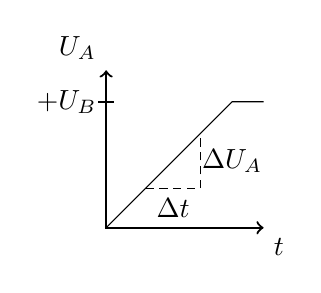
\begin{tikzpicture}
        \draw[thick,->] (-0.015,0) -- (2,0) node[anchor=north west] {$t$};
        \draw[thick,->] (0,0) -- (0,2) node[anchor=south east] {$U_{A}$};
        \draw (0,0) -- (1.6,1.6) -- (2,1.6);
        \draw[thick] (-0.1,1.6) -- (0.1,1.6);
        \draw (0,1.6) node[anchor=east] {$+U_B$};
        
        \draw[densely dashed] (0.5,0.5) -- (1.2,0.5) -- ++(0,0.7);  % Steigungsdreieck Linien
            \node at (1.6,0.85) {$\Delta U_A$};
            \node at (0.85,0.25) {$\Delta t$}; 
    \end{tikzpicture}} \\
    \hline
\end{tabular}}}{Schaltung des Beispielproblems mit einer Signalquelle auf der Eingangsseite und einer komplexen Last auf der Ausgangsseite \label{fig:Beispielproblem 1 Folien 2 Abbildung 1}} 
        }
    \end{frame}
    \begin{frame}
        \b{
            \frametitle{Prinzip der Gegenkopplung - Lösung des Beispielproblems (2)}
             \fu{\resizebox{0.8\textwidth}{!}{\begin{tabular}{|m{0.25\textwidth}|m{0.5\textwidth}|m{0.25\textwidth}|}
    \hline
    \begin{circuitikz}[scale=0.8, transform shape]
        \ctikzset{tripoles/en amp/input height=-0.45}
        \draw (0,0) node[en amp](E){};
        \node at ($(E) + (-1.2, 1.5)$) {\textbf{\LARGE A}}; % Label für den ersten OPV
        \draw (E.out) node[circ]{} node[right]{$U_A$};
        \draw (E.-) node[circ]{} node[left]{0V};
        \draw (E.+) node[circ]{} node[left]{1V};
        \draw (E.up) -- ++(0,0.5) node[anchor=south]{$+U_B$} node[circ] {};
        \draw (E.down) -- ++(0,-0.5) node[anchor=north]{$-U_B$} node[circ] {};
    \end{circuitikz} &
    \begin{circuitikz}[scale=0.8, transform shape]
        \ctikzset{tripoles/en amp/input height=-0.45}
        \draw (0,0) node[en amp](E){};
        \node at ($(E) + (-1.2, 1.5)$) {\textbf{\LARGE B}}; % Label für den ersten OPV im mittleren Bild
        \draw (E.out) node[circ]{} node[right]{$U_A$};
        \draw (E.-) node[circ]{} node[left]{0V} -- ++(0, -1) to[normal open switch] ++(2.38,0) -- ++(0,1.5);
        \draw (E.+) node[circ]{} node[left]{1V};
    
        \draw (4,0) node[en amp](E2){};
        \node at ($(E2) + (-1.2, 1.5)$) {\textbf{\LARGE C}}; % Label für den zweiten OPV im mittleren Bild
        \draw (E2.out) node[circ]{} node[right]{$U_A$};
        \draw (E2.-) node[circ]{} node[left]{0V} -- ++(0, -1) -- ++(2.38,0) -- ++(0,1.5);
        \draw (E2.+) node[circ]{} node[left]{1V};
    \end{circuitikz}
    \\
    \hline
    \multicolumn{1}{|c|}{
    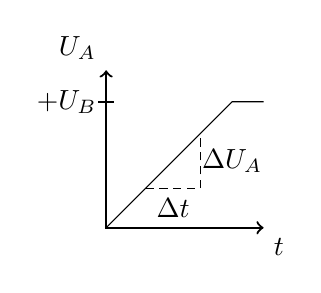
\begin{tikzpicture}
        \draw[thick,->] (-0.015,0) -- (2,0) node[anchor=north west] {$t$};
        \draw[thick,->] (0,0) -- (0,2) node[anchor=south east] {$U_{A}$};
        \draw (0,0) -- (1.6,1.6) -- (2,1.6);
        \draw[thick] (-0.1,1.6) -- (0.1,1.6);
        \draw (0,1.6) node[anchor=east] {$+U_B$};
        
        \draw[densely dashed] (0.5,0.5) -- (1.2,0.5) -- ++(0,0.7);  % Steigungsdreieck Linien
            \node at (1.6,0.85) {$\Delta U_A$};
            \node at (0.85,0.25) {$\Delta t$}; 
    \end{tikzpicture}} &
    \multicolumn{1}{c|}{
    \begin{tikzpicture}
        \draw[thick,->] (1.985,0) -- (4,0) node[anchor=north west] {$t$};
        \draw[thick,->] (2,0) -- (2,2) node[anchor=south east] {$U_{A}$};
        \draw (2,0) -- (3,0.5) -- (4,0.5);
        \draw[thick] (1.9,0.5) -- (2.1,0.5) node[anchor=east] {$1V$};
        \node at (0,1) {Slew rate: $\frac{\Delta U_A}{\Delta t}$};
    \end{tikzpicture}}
    \\
    \hline
    \end{tabular}}}{Schaltung des Beispielproblems mit einer Signalquelle auf der Eingangsseite und einer komplexen Last auf der Ausgangsseite \label{fig:Beispielproblem 1 Folien 2 Abbildung 2}} 
        }
    \end{frame}

%\speech{
% Beispiel 3.1: Teil 1: Entwicklung einer Verstärkerschaltung für Musiksignale.
% Bei der Entwicklung von Hi-Fi-Geräten müssen Verstärker an die Last (also den Lautsprecher) angepasst werden.
% Dazu wird ein Leistungsverstärker (d.h. eine Endstufe) benötigt. Eine solche Endstufe, die geeignet ist, das Signal eines Handys so zu verstärken, dass ein Lautsprecher damit betrieben werden kann soll hier aufgebaut werden.
% Ein vereinfachtes Ersatzschaltbild des Lautsprechers ist durch eine Induktivität mit einem in Reihe geschalteten Widerstand gegeben (siehe Abbildung \ref{fig:Beispielproblem 1}).
% Das Eingangsspannungsniveau ist 1~V und es soll ein 4~$\mathrm{\Omega}$ Lautsprecher betrieben werden (4~$\mathrm{\Omega}$ bedeutet, dass der Lautsprecher bei 1~kHz eine Impedanz von 4~$\Omega$ aufweist).
% Wie groß muss die Spannung am Ausgang des Verstärkers sein, damit der Lautsprecher bei 1~kHz 25 W aufnimmt? Wie kann hier vorgegangen werden, wenn eine Operationsverstärkerschaltung für die Lösung genutzt werden soll?
% Lösung: Zunächst muss dazu die Spannung berechnet werden, die der Verstärker ausgeben soll.
% U A = sqrt(P * R) = sqrt(25 W * 4 $\Omega$) = 10 V
% Wie kann nun mithilfe eines Operationsverstärkers der mit einem ? gekennzeichneten Teil der Schaltung ersetzt werden, um eine notwendige Verstärkung von 10 zu erreichen (siehe Abbildung \ref{fig:Beispielproblem 1})?
%} 

%\speech{
%Abbildung 3.1 zeigt eine Schaltung mit einer Signalquelle auf der Eingangsseite und einer komplexen Last auf der Ausgangsseite.  
%Die Signalquelle liefert eine Wechselspannung mit einer Amplitude von 1 Volt.  
%Das Signal wird an eine unbekannte Schaltung weitergeleitet, die durch ein Fragezeichen gekennzeichnet ist.  
%Diese Schaltung verstärkt oder verändert das Signal und gibt es an die Ausgangslast weiter.  
%
%Die Ausgangslast ist in einem gestrichelten Rechteck markiert und stellt ein Ersatzschaltbild für einen Lautsprecher dar.  
%Diese Last besteht aus einem Widerstand von 2 Ohm in Reihe mit einer Induktivität von 100 Millihenry.  
%Die Induktivität beeinflusst das Verhalten der Last in Abhängigkeit von der Frequenz des Eingangssignals.  
%
%Die Aufgabe besteht darin, den Verstärkungsfaktor der unbekannten Schaltung zu bestimmen.  
%Der Verstärkungsfaktor ist definiert als das Verhältnis der Ausgangsspannung U A zur Eingangsspannung U E.  
%Mathematisch ausgedrückt als V gleich U A geteilt durch U E.  
%
%Um den Verstärkungsfaktor zu berechnen, müssen die Eigenschaften der unbekannten Schaltung sowie die Auswirkungen der komplexen Last berücksichtigt werden.  
%}



\begin{frame}
    \s{\pagebreak
        Wie aus vorherigen Kapiteln bekannt ist, besitzen Operationsverstärker einen invertierenden und einen nicht-invertierenden Eingang. Existiert zwischen diesen beiden Eingängen eine Spannungsdifferenz, so verstärkt der Operationsverstärker diese Differenz um ein Vielfaches, bis die Spannung die maximale Ausgangsspannung des Operationsverstärkers erreicht (siehe A in Abbildung \ref{fig: Verschaltung Verstaerker}).
    Die Slew-Rate (zu deutsch: Anstiegsrate) gibt an, wie schnell dieser Anstieg geschehen kann. Wird die Ausgangsspannung nicht auf den Eingang zurückgeführt, steigt die Ausgangspannung, bis das Niveau der Versorgungsspannung erreicht wird. Eine solche Beschaltung des Verstärkers wird als Komperatorschaltung bezeichet.

    Dieses Verhalten ist für die meisten Anwendungen bei denen der Eingangsspannungssignal mit geringer Amplitude verstärkt werden soll, nicht erwünscht. 
    Stattdessen werden Operationsverstärker meistens in der sogenannten Gegenkopplung (B) betrieben, bei der der Ausgang auf den invertierenden Eingang zurückgeführt wird. 
    Der in (B) eingezeichnete Schalter sei zunächst geöffnet und der Operationsverstärker werde nicht mit Spannung versorgt. Zum Zeitpunkt 0 s wird der Schalter geschlossen und die Versorgungsspannung des Verstärkers eingeschaltet, wodurch die Rückführung des Ausgangssignals $U_{\textnormal{A}}$ aktiv wird (C). 
    Durch die Rückkopplung des Ausgangssignal wird so erreicht, dass die Spannung am invertierenden Eingang auf das Spannungsniveau der Ausgangsspannung angeglichen wird. 
    Die in (C) dargestellte Verstärkerschaltung hat die Verstärkung 1 und wird als Impedanzwandler bezeichnet, da der Verstärker in dieser Schaltungsart aufgrund seiner hohen Eingangsimpedanz verwendet werden kann, um eine Schaltung mit hochohmigem Eingang zu realisieren (dies ist beispielsweise bei Messschaltungen für Spannungsmessungen notwendig). 
    Für die Lösung des Anwendungsproblems ist diese Schaltung allerdings noch nicht geeignet, da eine Verstärkung von 5 gefordert ist. 
    Um diese zu erreichen werden in die Verstärkerschaltung nun zusätzlich Widerstände eingebaut (wie in (D) dargestellt ist)\footnote{Es lässt sich feststellen, dass sich für $R_2 = 0$ und $R_1 = \infty$ wieder die Schaltung des Impedanzwandlers ergibt. Der Impedanzwandler ist also ein Spezialfall des nicht-invertierenden Verstärkers.}.      
    }
    \b{\frametitle{Prinzip der Gegenkopplung - Lösung des Beispielproblems (2)}}
    \fu{
        \resizebox{\textwidth}{!}{\begin{tabular}{|m{0.25\textwidth}|m{0.45\textwidth}|m{0.3\textwidth}|}
    \hline
    \begin{circuitikz}[scale=0.8, transform shape]
        \ctikzset{tripoles/en amp/input height=-0.45}
        \draw (0,0) node[en amp](E){};
        \node at ($(E) + (-1.2, 1.5)$) {\textbf{\LARGE A}}; % Label für den ersten OPV
        \draw (E.out) node[circ]{} node[right]{$U_A$};
        \draw (E.-) node[circ]{} node[left]{0V};
        \draw (E.+) node[circ]{} node[left]{1V};
        \draw (E.up) -- ++(0,0.5) node[anchor=south]{$+U_B$} node[circ] {};
        \draw (E.down) -- ++(0,-0.5) node[anchor=north]{$-U_B$} node[circ] {};

    \end{circuitikz} &
    \begin{circuitikz}[scale=0.8, transform shape]
        \ctikzset{tripoles/en amp/input height=-0.45}
        \draw (0,0) node[en amp](E){};
        \node at ($(E) + (-1.2, 1.5)$) {\textbf{\LARGE B}}; % Label für den ersten OPV im mittleren Bild
        \draw (E.out) node[circ]{} node[right]{$U_A$};
        \draw (E.-) node[circ]{} node[left]{0V} -- ++(0, -1) to[normal open switch] ++(2.38,0) -- ++(0,1.5);
        \draw (E.+) node[circ]{} node[left]{1V};
    
        \draw (4,0) node[en amp](E2){};
        \node at ($(E2) + (-1.2, 1.5)$) {\textbf{\LARGE C}}; % Label für den zweiten OPV im mittleren Bild
        \draw (E2.out) node[circ]{} node[right]{$U_A$};
        \draw (E2.-) node[circ]{} node[left]{0V} -- ++(0, -1) -- ++(2.38,0) -- ++(0,1.5);
        \draw (E2.+) node[circ]{} node[left]{1V};
    \end{circuitikz} &
    \begin{circuitikz}[scale=0.8, transform shape]
        \ctikzset{tripoles/en amp/input height=-0.45,
        }
        \draw (0,0) node[en amp](E){};
        \node at ($(E) + (-1.2, 1.5)$) {\textbf{\LARGE D}}; % Label für den OPV im dritten Bild
        \draw (E.out) node[circ]{} -- ++(0.2,0) node[ocirc, right]{};
        \draw (E.-) -- ++(0, -1.3) node[circ] {} to[R, l=$R_2$] ++(2.38,0) -- ++(0,1.8);
        \draw (E.-) -- ++(0, -1.6) to[R, l_=$R_1$] ++(0, -1.2) -- ++(0,-0.2) -- ++(-0.2, 0) -- ++(0.4,0);
        \draw (E.+) node[circ]{} node[left]{};     
       
        % Spannungspfeil
        \draw[-{Triangle[width=3pt,length=4pt]}, color=spannung] ($(E.+) + (0, -0.1)$) -- ($(E.-) + (0, 0.1)$) node[midway, xshift=-30] {$U_{\text{Diff}}=0\,\text{V}$};
        \draw[-{Triangle[width=3pt,length=4pt]}, color=spannung] ($(E.out) + (0.26, -0.1)$) -- ($(E.out) + (0.26, -3.45)$) node[midway, xshift=10] {$U_A$};
        \draw[black] ($(E.out) + (0.26, -3.5)$) -- ++(-0.2, 0) -- ++(0.4,0);
        \draw[-{Triangle[width=3pt,length=4pt]}, color=spannung] (0.7,-2.1)-- ++(-1.5,0) node[midway, yshift=-10] {$U_{R2}$};
        \draw[-{Triangle[width=3pt,length=4pt]}, color=spannung] (-0.9,-2)-- ++(0,-1.5) node[midway, xshift=10] {$U_{R1}$};


        
        \node[red] at (0.9,-1.8) {\tikz \draw[red, -{Triangle[width=3pt,length=4pt]}] (0,0) -- (-0.01,0);};
        \node[above, color=red] at (0.9,-1.8)  {$I_{R2}$};

        \node[red] at ($(E.-)+(0,-1.5)$) {\tikz \draw[red, -{Triangle[width=3pt,length=4pt]}] (0,0) -- (0,-0.01);};
        \node[left, color=red] at ($(E.-)+(0,-1.4)$)  {$I_{R1}$};
    \end{circuitikz}
    \\
    \hline
    \multicolumn{1}{|c|}{
    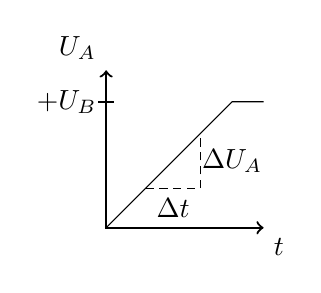
\begin{tikzpicture}
        \draw[thick,->] (-0.015,0) -- (2,0) node[anchor=north west] {$t$};
        \draw[thick,->] (0,0) -- (0,2) node[anchor=south east] {$U_{A}$};
        \draw (0,0) -- (1.6,1.6) -- (2,1.6);
        \draw[thick] (-0.1,1.6) -- (0.1,1.6);
        \draw (0,1.6) node[anchor=east] {$+U_B$};
        
        \draw[densely dashed] (0.5,0.5) -- (1.2,0.5) -- ++(0,0.7);  % Steigungsdreieck Linien
            \node at (1.6,0.85) {$\Delta U_A$};
            \node at (0.85,0.25) {$\Delta t$}; 
    \end{tikzpicture}} &
    \multicolumn{1}{c|}{
    \begin{tikzpicture}
        \draw[thick,->] (1.985,0) -- (4,0) node[anchor=north west] {$t$};
        \draw[thick,->] (2,0) -- (2,2) node[anchor=south east] {$U_{A}$};
        \draw (2,0) -- (3,0.5) -- (4,0.5);
        \draw[thick] (1.9,0.5) -- (2.1,0.5) node[anchor=east] {$1V$};
        \node at (0,1) {Slew rate: $\frac{\Delta U_A}{\Delta t}$};
    \end{tikzpicture}} &
    \multicolumn{1}{c|}{
    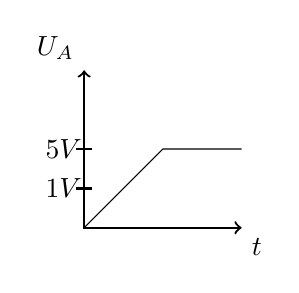
\begin{tikzpicture}
        \draw[thick,->] (-0.015,0) -- (2,0) node[anchor=north west] {$t$};
        \draw[thick,->] (0,0) -- (0,2) node[anchor=south east] {$U_{A}$};
        \draw (0,0) -- (1,1) -- (2,1);
        \draw[thick] (-0.1,1) -- (0.1,1) node[anchor=east] {$5V$};
        \draw[thick] (-0.1,0.5) -- (0.1,0.5) node[anchor=east] {$1V$};
    \end{tikzpicture}} \\
    \hline
    \end{tabular}}
        }{Verschaltung eines Verstärkers als Komperator (A), Impedanzwandler (C) und nicht-invertierender Verstärker (D)
        \label{fig: Verschaltung Verstaerker}}       
\end{frame}

%\speech {
%    Wie aus vorherigen Kapiteln bekannt ist, besitzen Operationsverstärker einen invertierenden und einen nicht-invertierenden Eingang. Existiert zwischen diesen beiden Eingängen eine Spannungsdifferenz, so verstärkt der Operationsverstärker diese Differenz um ein Vielfaches, bis die Spannung die maximale Ausgangsspannung des Operationsverstärkers erreicht (siehe A in Abbildung \ref{fig: Verschaltung Verstaerker}).
%    Die Slew-Rate (zu deutsch: Anstiegsrate) gibt an, wie schnell dieser Anstieg geschehen kann. Wird die Ausgangsspannung nicht auf den Eingang zurückgeführt, steigt die Ausgangspannung, bis das Niveau der Versorgungsspannung erreicht wird. Eine solche Beschaltung des Verstärkers wird als Komperatorschaltung bezeichet.
% Dieses Verhalten ist für die meisten Anwendungen bei denen der Eingangsspannungssignal mit geringer Amplitude verstärkt werden soll, nicht erwünscht.
% Stattdessen werden Operationsverstärker meistens in der sogenannten Gegenkopplung (B) betrieben, bei der der Ausgang auf den invertierenden Eingang zurückgeführt wird.
% Der in (B) eingezeichnete Schalter sei zunächst geöffnet und der Operationsverstärker werde nicht mit Spannung versorgt. Zum Zeitpunkt 0 s wird der Schalter geschlossen und die Versorgungsspannung des Verstärkers eingeschaltet, wodurch die Rückführung des Ausgangssignals $U_{\textnormal{A}}$ aktiv wird (C).
% Durch die Rückkopplung des Ausgangssignal wird so erreicht, dass die Spannung am invertierenden Eingang auf das Spannungsniveau der Ausgangsspannung angeglichen wird.
% Die in (C) dargestellte Verstärkerschaltung hat die Verstärkung 1 und wird als Impedanzwandler bezeichnet, da der Verstärker in dieser Schaltungsart aufgrund seiner hohen Eingangsimpedanz verwendet werden kann, um eine Schaltung mit hochohmigem Eingang zu realisieren (dies ist beispielsweise bei Messschaltungen für Spannungsmessungen notwendig).
% Für die Lösung des Anwendungsproblems ist diese Schaltung allerdings noch nicht geeignet, da eine Verstärkung von 5 gefordert ist.
% Um diese zu erreichen werden in die Verstärkerschaltung nun zusätzlich Widerstände eingebaut (wie in (D) dargestellt ist)\footnote{Es lässt sich feststellen, dass sich für $R_2 = 0$ und $R_1 = \infty$ wieder die Schaltung des Impedanzwandlers ergibt. Der Impedanzwandler ist also ein Spezialfall des nicht-invertierenden Verstärkers.}.
%}
%\speech{
%Abbildung 3.2 zeigt verschiedene Verschaltungen eines Operationsverstärkers und deren zugehörige Ausgangsverläufe.  
%Es sind vier verschiedene Konfigurationen dargestellt:  
%Ein Komparator, zwei Varianten eines Impedanzwandlers und ein nichtinvertierender Verstärker.  
%
%Im oberen Bereich der Abbildung sind die jeweiligen Schaltungen zu sehen.  
%Im unteren Bereich sind die entsprechenden Ausgangsdiagramme dargestellt, die den zeitlichen Verlauf der Ausgangsspannung U A zeigen.  
%
%Schaltung A zeigt einen Operationsverstärker als Komparator.  
%Der nichtinvertierende Eingang erhält eine konstante Spannung von 1 Volt.  
%Der invertierende Eingang ist auf 0 Volt gelegt.  
%Da die Eingangsspannung am nichtinvertierenden Eingang größer ist, springt die Ausgangsspannung auf den maximalen positiven Wert.  
%Das untere Diagramm zeigt den Ausgangsverlauf als sprunghafte Änderung.  
%
%Schaltung B und C zeigen einen Operationsverstärker als Impedanzwandler, auch Unity-Gain-Buffer genannt.  
%Hierbei wird die Eingangsspannung direkt am nichtinvertierenden Eingang angelegt.  
%Der Ausgang ist mit dem invertierenden Eingang verbunden, sodass eine Verstärkung von Eins entsteht.  
%Das untere Diagramm zeigt, dass die Ausgangsspannung genau der Eingangsspannung folgt.  
%
%Schaltung D zeigt einen nichtinvertierenden Verstärker.  
%Ein Spannungsteiler aus den Widerständen R1 und R2 bestimmt die Verstärkung.  
%Die Ausgangsspannung U A ist größer als die Eingangsspannung.  
%Das untere Diagramm zeigt eine Verstärkung des Signals, wobei die Ausgangsspannung von 1 Volt auf 5 Volt ansteigt.  
%
%Die Abbildung zeigt, wie sich unterschiedliche Verschaltungen auf die Ausgangsspannung auswirken.  
%}

\begin{frame}
    \s{
    \begin{bsp}{Teil 2: Entwicklung einer Verstärkerschaltung für Musiksignale}{Beispiel Verstaerkung 2}
        Im letzten Schritt muss ermittelt werden, wie die Widerstände in (D) gewählt werden müssen, damit sich eine Verstärkung von 5 ergibt. Dazu müssen zunächst die Maschengleichungen aufgestellt werden.
        Eine wichtige Annahme zur Aufstellung dieser Maschengleichung ist, dass davon ausgegangen wird, dass der Verstärker durch die Rückkopplung des Ausgangsignal die beiden Eingangssignale angleicht. 
        Hier darf also geschrieben werden \glqq Annahme: $U_{\textnormal{dif}}~=~0$~V\grqq{}. 
        Somit ergibt sich für den invertierenden Eingang $U_{\textnormal{E-}}~=~1$~V.
        Da weiterhin davon ausgegangen wird, dass kein Strom in die Eingänge hineinfließt gilt $I_{\textnormal{R1}}~=~I_{\textnormal{R2}}$.
        Die Maschengleichung lautet auf Grundlage dieser Annahmen
        \begin{equation}
            U_{\textnormal{A}} = U_{\textnormal{R1}} + U_{\textnormal{R2}} = U_{\textnormal{E}} + I_{\textnormal{R2}} \cdot R_{\textnormal{2}} = U_{\textnormal{E}} + \frac{U_{\textnormal{E}}}{R_{\textnormal{1}}} \cdot R_{\textnormal{2}} 
        \end{equation}

        Dadurch ergibt sich das Ein-Ausgangsverhalten im zeitbereich zu folgendem Ausdruck.
        \begin{equation}
            \frac{U_{\textnormal{A}}}{U_{\textnormal{E}}} = \underbrace{(1+\frac{R_2}{R_1})}_{V}
        \end{equation}
        

        Wird diese Gleichung nach $R_2/R_1$ gelöst, ergibt sich das Verhältnis der Widerstände für das oben beschriebene 
        Problem zu $R_2/R_1 = 9$. Die Widerstände sollten hier nicht zu groß gewählt werden, da dann der Ausgleichsstrom zwischen
        Ausgang und Eingang zu klein werden könnte. Das kann zu einem starken Rauschen am Verstärkerausgang führen. Übliche Widerstandswerte sind in der Regel den Beispielschaltungen des Datenblattes eines
        Operationsverstärkers zu entnehmen. In diesem Fall könnte z.B. $R_2=9~\textnormal{k}\Omega$ und $R_1=1~\textnormal{k}\Omega$ gewählt werden.
    \end{bsp} 

%\speech{1}{
%Beispiel 3.2: Teil 2: Entwicklung einer Verstärkerschaltung für Musiksignale.
%Im letzten Schritt muss ermittelt werden, wie die Widerstände in (D) gewählt werden müssen, damit sich eine Verstärkung von 5 ergibt. Dazu müssen zunächst die Maschengleichungen aufgestellt werden.
%Eine wichtige Annahme zur Aufstellung dieser Maschengleichung ist, dass davon ausgegangen wird, dass der Verstärker durch die Rückkopplung des Ausgangsignal die beiden Eingangssignale angleicht.
%Hier darf also geschrieben werden \glqq Annahme: $U_{\textnormal{dif}}~=~0$~V\grqq{}.
%Somit ergibt sich für den invertierenden Eingang $U_{\textnormal{E-}}~=~1$~V.
%Da weiterhin davon ausgegangen wird, dass kein Strom in die Eingänge hineinfließt gilt $I_{\textnormal{R1}}~=~I_{\textnormal{R2}}$.
%Die Maschengleichung lautet auf Grundlage dieser Annahmen
%\begin{equation}
%    U_{\textnormal{A}} = U_{\textnormal{R1}} + U_{\textnormal{R2}} = U_{\textnormal{E}} + I_{\textnormal{R2}} \cdot R_{\textnormal{2}} = U_{\textnormal{E}} + \frac{U_{\textnormal{E}}}{R_{\textnormal{1}}} \cdot R_{\textnormal{2}}
%\end{equation}
%Wird diese Gleichung nach $R_2/R_1$ gelöst, ergibt sich das Verhältnis der Widerstände für das oben beschriebene 
%Problem zu $R_2/R_1 = 9$. Die Widerstände sollten hier nicht zu groß gewählt werden, da dann der Ausgleichsstrom zwischen
%Ausgang und Eingang zu klein werden könnte. Das kann zu einem starken Rauschen am Verstärkerausgang führen. Übliche Widerstandswerte sind in der Regel den Beispielschaltungen des Datenblattes eines
%Operationsverstärkers zu entnehmen. In diesem Fall könnte z.B. $R_2=9~\textnormal{k}\Omega$ und $R_1=1~\textnormal{k}\Omega$ gewählt werden.
%}
        \par
        Ähnnlich wie für die oben dargestellte Schaltung lassen sich auch für alle weiteren Operationsverstärkerschaltungen Übertragungsfunktionen herleiten. Das soll hier allerdings nicht gezeigt werden.
        Weitere Übertragungsfuktionen für einige ausgewählte Operationsverstärkergrundschaltungen können Tabelle \ref{tab:Grundschaltungen} entnommen werden. 
        In dieser Tabelle sind die die Schaltungen, die Bodediagramme mit Phasengang (rot) und Amplitudengang (blau) und die Übertragungsfunktionen angegeben. 
        Nachdem nun die Beschaltung von Verstärkern vorgestellt wurde, soll im Folgenden Kapitel nun noch eine wichtige Eigenschaft von Verstärkerschaltungen thematisiert werden, die sich aus den genutzen Verstärkerbausteinen und der äußeren Verschaltung ergibt: Die Stabilität der Verstärkerschaltung.
        
%\speech {1}{
% Ähnlich wie für die oben dargestellte Schaltung lassen sich auch für alle weiteren Operationsverstärkerschaltungen Übertragungsfunktionen herleiten. Das soll hier allerdings nicht gezeigt werden.
%    Weitere Übertragungsfuktionen für einige ausgewählte Operationsverstärkergrundschaltungen können Tabelle \ref{tab:Grundschaltungen} entnommen werden.
%    In dieser Tabelle sind die die Schaltungen, die Bodediagramme mit Phasengang (rot) und Amplitudengang (blau) und die Übertragungsfunktionen angegeben.
%    Nachdem nun die Beschaltung von Verstärkern vorgestellt wurde, soll im Folgenden Kapitel nun noch eine wichtige Eigenschaft von Verstärkerschaltungen thematisiert werden, die sich aus den genutzen Verstärkerbausteinen und der äußeren Verschaltung ergibt: Die Stabilität der Verstärkerschaltung.   
%}
        
%\speech{
%Tabelle 3.1 zeigt verschiedene Grundschaltungen mit Operationsverstärkern.  
%Die Tabelle ist in drei Spalten unterteilt.  
%Die erste Spalte zeigt die Schaltung, die zweite Spalte enthält den Frequenzgang und die Gleichung,  
%und die dritte Spalte gibt eine Erklärung mit den wichtigsten Eigenschaften.  
%
%Erste Zeile: Nichtinvertierender Verstärker.  
%Die Ausgangsspannung ist phasengleich mit der Eingangsspannung.  
%Die Verstärkung ist eins plus das Verhältnis von R2 zu R1.  
%Der Verstärker hat einen sehr hohen Eingangswiderstand und einen niedrigen Ausgangswiderstand.  
%Anwendungsbeispiel ist ein Impedanzwandler.  
%
%Zweite Zeile: Invertierender Verstärker.  
%Die Ausgangsspannung ist um 180 Grad phasenverschoben zur Eingangsspannung.  
%Die Verstärkung ist das Verhältnis von R2 zu R1.  
%Der Widerstand R1 bestimmt den Eingangswiderstand.  
%Anwendungsbeispiel ist ein aktiver Spannungsteiler für hohe Spannungen.  
%
%Dritte Zeile: Komparator.  
%Die Ausgangsspannung ist entweder hoch oder niedrig, je nach Vergleich der Eingänge.  
%Wenn die nichtinvertierende Spannung größer ist als die invertierende Spannung,  
%geht die Ausgangsspannung auf den oberen Versorgungswert.  
%Andernfalls geht sie auf den unteren Versorgungswert.  
%Wird verwendet in Zweipunktreglern und Analog-Digital-Wandlern.  
%
%Vierte Zeile: Summierer.  
%Der Summierer basiert auf einem invertierenden Verstärker.  
%Die Ausgangsspannung ist eine gewichtete Summe mehrerer Eingangsspannungen.  
%Wird verwendet in Analogrechnern und zur Mischung von Signalen.  
%
%Fünfte Zeile: Subtrahierer.  
%Diese Schaltung bildet die Differenz zwischen zwei Eingangsspannungen.  
%Wenn alle Widerstände gleich sind, entspricht die Ausgangsspannung genau der Differenz der Eingänge.  
%Diese Schaltung wird als Differenzverstärker verwendet.  
%
%Sechste Zeile: Integrierer.  
%Der Integrierer summiert die Eingangsspannung über die Zeit.  
%Die Ausgangsspannung entspricht dem negativen Integral des Eingangssignals.  
%Wird als aktiver Tiefpassfilter verwendet.  
%
%Siebte Zeile: Differenzierer.  
%Der Differenzierer bildet die Ableitung des Eingangssignals.  
%Die Ausgangsspannung ist proportional zur zeitlichen Änderung der Eingangsspannung.  
%Wird als Hochpassfilter eingesetzt, zeigt in der Praxis aber oft ein Bandpassverhalten.  
%
%Diese Tabelle gibt einen Überblick über wichtige Operationsverstärkerschaltungen  
%und ihre typischen Anwendungen in der Signalverarbeitung.  
%}



        \begin{block}{}
            \begin{table}[ht]
    \caption{Ausgewählte Operationsverstärker-Grundschaltungen}
    \label{tab:Grundschaltungen}
    \begin{tabular}{|m{0.24\textwidth}|m{0.405\textwidth}|m{0.33\textwidth}|}
    \hline
    Schaltung & Frequenzgang und Gleichung & Erläuterung und Eigenschaften\\ % Neue Zeile mit Text
    \hline
    \vspace{0.5cm}
    \centering
    \begin{circuitikz}[scale=0.7, transform shape]
    \ctikzset{
         resistors/scale=0.8,              
         tripoles/en amp/height=1.4, % Höhe des OPV             
         tripoles/en amp/width=1.4,   % Breite des OPV
         tripoles/en amp/input height=-0.45
    }
    \vspace{1ex}
    \draw (2,-0.1) node[en amp] (opamp) {}
    (opamp.+) --++ (-0.5,0) node[ocirc, label=left:$U_E$] (eingang) {} 
    (opamp.out) --++ (0.5,0) node[ocirc, label=right:$U_A$] {}
    (opamp.-) -- ++(0, -1.5) to[R, l=$R_1$] ++(0, -1) node[ground] {}
    (opamp.out) node[circ] {} -- ++(0,-1.5) to[R, l=$R_2$] ++(-1.95,0) node[circ] (feedback) {};
\end{circuitikz}

 & \begin{tikzpicture}[scale=1, transform shape]
    \begin{axis}[
    width=4.5cm, % Breite des Graphen
    height=3.5cm, % Höhe des Graphen
    xmin=0, xmax=10,
    ymin=0, ymax=120,
    axis lines=left,
    axis on top=true,
    domain=0:10,
    xtick=\empty,
    ytick=\empty,
    ylabel style={rotate=270, anchor=east, yshift=1cm}, % Position der Beschriftung oben links, horizontal
     ylabel={\it V}, % Hier die gewünschte Beschriftung einfügen
    xlabel={f[Hz]},
    clip mode=individual % Verhindert das Abschneiden von Elementen
    ]
    \path[draw=none] (axis cs:-4, 0) rectangle (axis cs:16.6,120);
    
    
    \coordinate (xaxis) at (axis description cs:15.5,0); % Verwendet die relative Positionierung für x-Achse
    
    \addplot+[mark=none, thick, blue] coordinates {(0,80) (10,80)};
    % Adding the left-side label
    \node[anchor=east] at (axis cs:0,80) {$1 + \frac{R_2}{R_1}$};
    \end{axis}
    \begin{axis}[
    width=4.5cm, % Breite des Graphen
    height=3.5cm, % Höhe des Graphen
    xmin=0, xmax=10,
    ymin=-180, ymax=180,
    axis y line*=right,
    axis x line=none,
    ytick=\empty,
    ylabel={$\varphi$},
    ylabel style={rotate=270, anchor=west, yshift=0.8cm},
    clip mode=individual, % Verhindert das Abschneiden von Elementen
    after end axis/.code={
        \draw[->] (axis cs:10,180) -- (axis cs:10,190);
    }
    ]
    \addplot+[mark=none, thick, red] coordinates {(0,0) (10,0)};
    \node[anchor=west] at (axis cs:10,0) {$0^\circ$};
    \end{axis}
    \end{tikzpicture}
\vspace{1ex}
\[
U_{\textnormal{A}} = \left(1+\frac{R_2}{R_1}\right) U_{\textnormal{E}}
\]
    &
    \textbf{Nicht-invertierender Verstärker}
\begin{itemize}
    \item Phasengleiches Ausgangs-\linebreak signal
    \item Sehr hochohmiger Eingangswiderstand
    \item Niederohmiger Ausgangs-\linebreak widerstand
    \item Anwendungen: z.B. Impedanzwandler
\end{itemize} \\
    \hline
    \centering
    \begin{circuitikz}[scale=0.7, transform shape]
    \ctikzset{
          resistors/scale=0.8,              
          tripoles/en amp/height=1.4, % Höhe des OPV             
          tripoles/en amp/width=1.4,   % Breite des OPV
         tripoles/en amp/input height=0.45
     }
     \draw
     (0,0) node[en amp] (opamp) {}
     (opamp.-) to[R, l_=$R_1$, *-] ++(-1.2,0) to[short, o-] ++(0,0) node[left] {$U_E$}
     (opamp.+) -- ++(0,0) node[ground] {}
     (opamp.-) |- ++(0,1) to[R, l=$R_2$] ++(1.9,0) -| (opamp.out)
     (opamp.out) to[short, *-o] ++(0.2,0) node[right] {$U_{A}$};
 \end{circuitikz}
     & 
    \begin{center}
        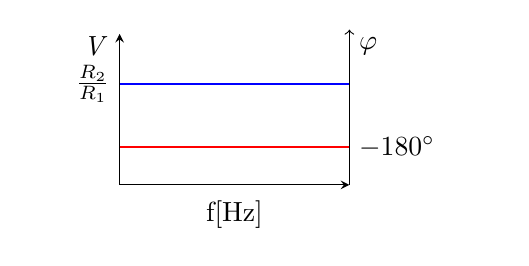
\begin{tikzpicture}[scale=1, transform shape]
    \begin{axis}[
        width=4.5cm, % Breite des Graphen
        height=3.5cm, % Höhe des Graphen
        xmin=0, xmax=10,
        ymin=0, ymax=120,
        axis lines=left,
        axis on top=true,
        domain=0:10,
        xtick=\empty,
        ytick=\empty,
        ylabel style={rotate=270, anchor=east, yshift=0.8cm},
         ylabel={\it V},
        xlabel={f[Hz]},
        clip mode=individual % Verhindert das Abschneiden von Elementen
        ]
        \path[draw=none] (axis cs:-4, 0) rectangle (axis cs:16.6,120);
    
        \addplot+[mark=none, thick, blue] coordinates {(0,80) (10,80)};
        % Adding the left-side label
        \node[anchor=east] at (axis cs:0,80) {$\frac{R_2}{R_1}$};
    \end{axis}
    \begin{axis}[
        width=4.5cm, % Breite des Graphen
        height=3.5cm, % Höhe des Graphen
        xmin=0, xmax=10,
        ymin=-180, ymax=180,
        axis y line*=right,
        axis x line=none,
        ytick=\empty,
        ylabel={$\varphi$},
        ylabel style={rotate=270, anchor=west, yshift=0.8cm},
        clip mode=individual, % Verhindert das Abschneiden von Elementen
        after end axis/.code={
            \draw[->] (axis cs:10,180) -- (axis cs:10,190);
        }
        ]
        \addplot+[mark=none, thick, red] coordinates {(0,-90) (10,-90)};
        \node[anchor=west] at (axis cs:10,-90) {$-180^\circ$};
    \end{axis}
    \end{tikzpicture}
\end{center}
\vspace{1ex}
\[
    U_{\textnormal{A}} = \frac{R_2}{R_1} U_{\textnormal{E}}
\]
    &
    \textbf{Invertierender Verstärker}
\begin{itemize}
    \item -180$^\circ$ Phasenverschiebung zwischen Ein- zu Ausgang
    \item $R_1$ bestimmt den Eingangswiderstand
    \item Niederohmiger Ausgangs-\linebreak widerstand
    \item Anwendungen: \linebreak z.B. Aktiver Spannungsteiler zum Messen hoher Spannungen, wenn $R_1 > R_2$
\end{itemize}
\\ % Zweite Zeile
    \hline
    \centering
    \begin{circuitikz}[scale=0.7, transform shape]
    \ctikzset{
          resistors/scale=0.8,              
          tripoles/en amp/height=1.4, % Höhe des OPV             
          tripoles/en amp/width=1.4,   % Breite des OPV
         tripoles/en amp/input height=0.45
     }
     \draw
     (0,0) node[en amp] (opamp) {}
     (opamp.-)  to[short, o-] ++(0,0) node[left] {$U_{E-}$}
      (opamp.+) to[short, o-] ++(0,0) node[left] {$U_{E+}$}
     (opamp.out) to[short, -o] ++(0,0) node[right] {$U_{A}$};
 \end{circuitikz}
    & 
    \begin{center}
               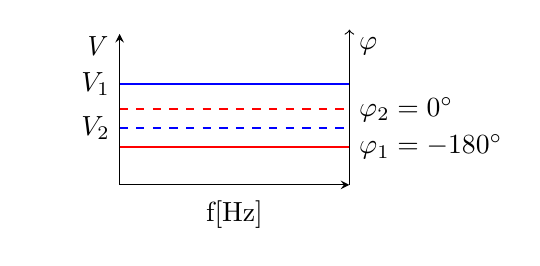
\begin{tikzpicture}[scale=1, transform shape]
    \begin{axis}[
        width=4.5cm, % Breite des Graphen
        height=3.5cm, % Höhe des Graphen
        xmin=0, xmax=10,
        ymin=0, ymax=120,
        axis lines=left,
        axis on top=true,
        domain=0:10,
        xtick=\empty,
        ytick=\empty,
        ylabel style={rotate=270, anchor=east, yshift=0.8cm},
         ylabel={\it V},
        xlabel={f[Hz]},
        clip mode=individual % Verhindert das Abschneiden von Elementen
        ]
        \path[draw=none] (axis cs:-4, 0) rectangle (axis cs:16.6,120);

        \addplot+[mark=none, thick, blue] coordinates {(0,80) (10,80)};
        \addplot+[mark=none, thick, blue, dashed] coordinates {(0,45) (10,45)};
        % Adding the left-side label
        \node[anchor=east] at (axis cs:0,80) {$V_1$};
        \node[anchor=east] at (axis cs:0,45) {$V_2$};
    \end{axis}
    \begin{axis}[
        width=4.5cm, % Breite des Graphen
        height=3.5cm, % Höhe des Graphen
        xmin=0, xmax=10,
        ymin=-180, ymax=180,
        axis y line*=right,
        axis x line=none,
        ytick=\empty,
        ylabel={$\varphi$},
        ylabel style={rotate=270, anchor=west, yshift=0.8cm},
        clip mode=individual, % Verhindert das Abschneiden von Elementen
        after end axis/.code={
            \draw[->] (axis cs:10,180) -- (axis cs:10,190);
        }
        ]
        \addplot+[mark=none, thick, red, dashed] coordinates {(0,0) (10,0)};
        \addplot+[mark=none, thick, red] coordinates {(0,-90) (10,-90)};
        \node[anchor=west] at (axis cs:10,0) {$\varphi_2 = 0^\circ$};
        \node[anchor=west] at (axis cs:10,-90) {$\varphi_1 = -180^\circ$};
    \end{axis}
    \end{tikzpicture}
\[
V_1: U_{\textnormal{E+}} > U_{\textnormal{E-}} \Rightarrow U_{\textnormal{A}} \approx +U_{\textnormal{B}}
\]
\[
V_2: U_{\textnormal{E+}} < U_{\textnormal{E-}} \Rightarrow U_{\textnormal{A}} \approx -U_{\textnormal{B}}
\]
\end{center}
    &\textbf{Komparator}\newline
    Einsatz in Zweipunktreglern und Analog-Digital-Wandlern
\\ % Dritte Zeile
    \hline

    

\centering
\begin{circuitikz}[scale=0.7, transform shape]
    \ctikzset{
        resistors/scale=0.8,              
        tripoles/en amp/height=1.4, % Höhe des OPV             
        tripoles/en amp/width=1.4,   % Breite des OPV
        tripoles/en amp/input height=0.45
    }
    \draw
    (0,0) node[en amp] (opamp) {}
    % R2 mit korrigiertem Strompfeil
    (opamp.-) -- ++(-0.4,0) node[circ] {} to[R, l_=$R_2$] ++(-1.5,0) node[ocirc] (R2left) {}
    % R1 mit korrigiertem Strompfeil
    (opamp.-) -- ++(-0.4,0) --++(0,1) to[R, l_=$R_1$] ++(-1.5,0) node[ocirc] (R1left) {}
    % Erdung
    (opamp.+) -- ++(0,0) node[ground] {}
    % Ausgang
    (opamp.out) to[short, *-o] ++(0,0) node[right] {$U_{A}$}
    % R3 mit Strompfeil
    (opamp.out) -- ++(0,1.5) to[R, l_=$R_3$] ++(-2,0) -- ++(0,-1.05) node[circ] {}
    % Spannungen U_E1 und U_E2 an den Knoten links von R1 und R2
    (R1left) node[left] {$U_{E1}$}
    (R2left) node[left] {$U_{E2}$};
\end{circuitikz}

    &
    \begin{center}
    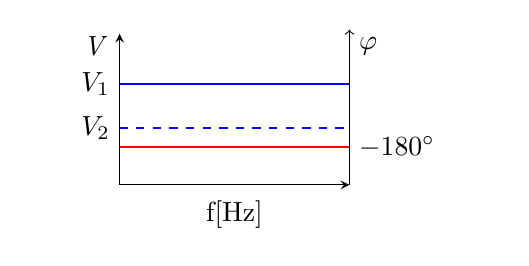
\begin{tikzpicture}[scale=1, transform shape]
    \begin{axis}[
        width=4.5cm, % Breite des Graphen
        height=3.5cm, % Höhe des Graphen
        xmin=0, xmax=10,
        ymin=0, ymax=120,
        axis lines=left,
        axis on top=true,
        domain=0:10,
        xtick=\empty,
        ytick=\empty,
        ylabel style={rotate=270, anchor=east, yshift=0.8cm},
         ylabel={\it V},
        xlabel={f[Hz]},
        clip mode=individual % Verhindert das Abschneiden von Elementen
        ]
        \addplot+[mark=none, thick, blue] coordinates {(0,80) (10,80)};
        \addplot+[mark=none, thick, blue, dashed] coordinates {(0,45) (10,45)};
    
        % Adding the left-side label
        \node[anchor=east] at (axis cs:0,80) {$V_1$};
        \node[anchor=east] at (axis cs:0,45) {$V_2$};
    \end{axis}
    \begin{axis}[
        width=4.5cm, % Breite des Graphen
        height=3.5cm, % Höhe des Graphen
        xmin=0, xmax=10,
        ymin=-180, ymax=180,
        axis y line*=right,
        axis x line=none,
        ytick=\empty,
        ylabel={$\varphi$},
        ylabel style={rotate=270, anchor=west, yshift=0.8cm},
        clip mode=individual, % Verhindert das Abschneiden von Elementen
        after end axis/.code={
            \draw[->] (axis cs:10,180) -- (axis cs:10,190);
        }
        ]
        \path[draw=none] (axis cs:-4, 0) rectangle (axis cs:16.6,120);
        \addplot+[mark=none, thick, red] coordinates {(0,-90) (10,-90)};
        \node[anchor=west] at (axis cs:10,-90) {$-180^\circ$};
    \end{axis}
    \end{tikzpicture}
\end{center}
\vspace{1ex}
\[
\begin{aligned}
    U_{\textnormal{A}} = \underbrace{\frac{R_3} {R_1}}_{V_1} \cdot U_{\textnormal{E1}} + \underbrace{\frac{R_3} {R_2}}_{V_2} \cdot U_{\textnormal{E2}}
\end{aligned}
\]
    & 
    \textbf{Summierer}\newline
    Der Summierer basiert auf dem invertierenden Verstärker und findet Verwendung in Analogrechnern und beim Mischen von Spannungssignalen
    \\ % Vierte Zeile
    \hline
    
    \end{tabular}
\end{table}


\newpage












\begin{table}[ht]
    \begin{tabular}{|m{0.23\textwidth}|m{0.44\textwidth}|m{0.33\textwidth}|}
     \hline 
    Schaltung & Frequenzgang und Gleichung & Erläuterung und Eigenschaften \\ % Neue Zeile mit Text
    \hline
    \begin{circuitikz}[scale=0.7, transform shape]
    \ctikzset{
          resistors/scale=0.8,              
          tripoles/en amp/height=1.4, % Höhe des OPV             
          tripoles/en amp/width=1.4,   % Breite des OPV
         tripoles/en amp/input height=0.45
     }
     \draw
     (0,0) node[en amp] (opamp) {}
     (opamp.-) to[R, l_=$R_1$, o-] ++(-1.2,0) to[short, o-] ++(0,0) node[left] {$U_{E1}$}
     (opamp.+) node[circ] {} to[R,  l_=$R_4$] ++(0,-1.5) node[ground] {}
     (opamp.-) node[circ] {} -- ++(0,1) to[R, l=$R_2$] ++(1.9,0) -| (opamp.out)
     (opamp.out) to[short, *-o] ++(0.2,0) node[right] {$U_{A}$}
     (opamp.+) to[R, l_=$R_3$, *-] ++(-1.2,0) to[short, o-] ++(0,0) node[left] {$U_{E2}$};
 \end{circuitikz}
      &
      \begin{center}
      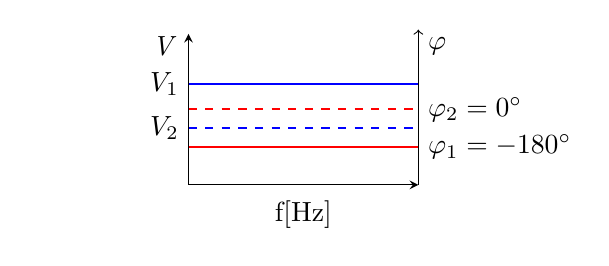
\begin{tikzpicture}[scale=1, transform shape]
    \begin{axis}[
        width=4.5cm, % Breite des Graphen
        height=3.5cm, % Höhe des Graphen
        xmin=0, xmax=10,
        ymin=0, ymax=120,
        axis lines=left,
        axis on top=true,
        domain=0:10,
        xtick=\empty,
        ytick=\empty,
        ylabel style={rotate=270, anchor=east, yshift=0.8cm},
         ylabel={\it V},
        xlabel={f[Hz]},
        clip mode=individual % Verhindert das Abschneiden von Elementen
        ]
        \addplot+[mark=none, thick, blue] coordinates {(0,80) (10,80)};
        \addplot+[mark=none, thick, blue, dashed] coordinates {(0,45) (10,45)};
        % Adding the left-side label
        \node[anchor=east] at (axis cs:0,80) {$V_1$};
        \node[anchor=east] at (axis cs:0,45) {$V_2$};
    \end{axis}
    \begin{axis}[
        width=4.5cm, % Breite des Graphen
        height=3.5cm, % Höhe des Graphen
        xmin=0, xmax=10,
        ymin=-180, ymax=180,
        axis y line*=right,
        axis x line=none,
        ytick=\empty,
        ylabel={$\varphi$},
        ylabel style={rotate=270, anchor=west, yshift=0.8cm},
        clip mode=individual, % Verhindert das Abschneiden von Elementen
        after end axis/.code={
            \draw[->] (axis cs:10,180) -- (axis cs:10,190);
        }
        ]
        \addplot+[mark=none, thick, red, dashed] coordinates {(0,0) (10,0)};
        \addplot+[mark=none, thick, red] coordinates {(0,-90) (10,-90)};
        \node[anchor=west] at (axis cs:10,0) {$\varphi_2 = 0^\circ$};
        \node[anchor=west] at (axis cs:10,-90) {$\varphi_1 = -180^\circ$};
   
   
        \path[draw=none] (axis cs:-7, 0) rectangle (axis cs:16.6,120);
   
   
   
   
    \end{axis}
    \end{tikzpicture}
 \end{center}
 \vspace{1ex}
 \[
 \begin{aligned}
    {U_A} = {U_{{\textnormal{E2}}}} \cdot \underbrace{ \frac{R_1 + R_2}{R_1} \cdot \frac{R_4}{R_3 + R_4}}_{V_2} - U_{\textnormal{E1}} \cdot \underbrace{\frac{R_2}{R_1}}_{V_1}
\end{aligned}
 \]
     &
     \textbf{Subtrahierer}\newline
     Wenn alle Widerstände gleich groß sind, wird die Differenz der Signale $U_{E1}$ und $U_{E2}$ gebildet, weswegen diese Schaltung als Differenzverstärker bezeichnet wird
 \\ % Fünfte Zeile
     \hline

    \begin{circuitikz}[scale=0.7, transform shape]
    \ctikzset{
          resistors/scale=0.8,              
          tripoles/en amp/height=1.4, % Höhe des OPV             
          tripoles/en amp/width=1.4,   % Breite des OPV
         capacitors/scale=0.5,
         tripoles/en amp/input height=0.45
     }
     \vspace{1ex}
     \draw (2,0) node[en amp] (opamp) {}
     (opamp.+) --++ (-0.5,0) node[ground] {} 
     (opamp.out) --++ (0.2,0) node[ocirc, label=right:$U_A$] {}
     (opamp.-) -- ++(0, 0) to[R, l_=$R_1$] ++(-1.2, 0) node[ocirc, label=left:$U_E$] {}
     
     (opamp.out) node[circ] {} -- ++(0,1.5) to[C, l_=$C_1$, *-] ++(-1.9,0) node[circ]{}
     (opamp.out) node[circ] {} -- ++(0,2.8) to[R, l_=$R_2$] ++(-1.9,0) -- ++(0, -2.35) node[circ] {};
     \end{circuitikz}
     & 
     \begin{center}
    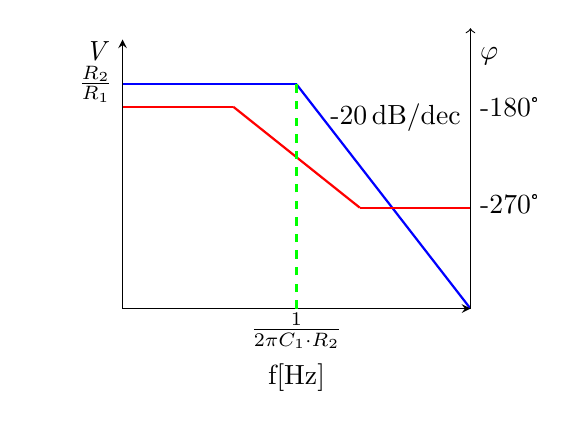
\begin{tikzpicture}[scale=1, transform shape]
    \begin{axis}[
       width=6cm, % Breite des Graphen
       height=5cm, % Höhe des Graphen
        xmin=0, xmax=11,
        ymin=0, ymax=1.2,
        axis lines=center,
        axis on top=true,
        domain=0:10,
        xtick=\empty,
        ytick=\empty,
        ylabel style={xshift=-0.6cm, yshift=0.1cm },
       ylabel={\it V},
       xlabel style={yshift=-0.4cm },
        xlabel={f[Hz]},
        clip mode=individual, % Verhindert das Abschneiden von Elementen
        xlabel style={at={(axis description cs:0.5,-0.05)},anchor=north}
        ]

        \path[draw=none] (axis cs:-3, 0) rectangle (axis cs:13,1);



        \addplot+[mark=none, thick, blue] coordinates {(0,1) (5.5,1)};
        \addplot+[mark=none, thick, blue] coordinates {(5.5,1) (11,0)};
        \node[anchor=east] at (axis cs:0,1) {$\frac{R_2}{R_1}$};
       \node[anchor=east] at (axis cs:11,0.85) {-20\,\text{dB/dec}};
    \end{axis}
    
    \begin{axis}[
       width=6cm, % Breite des Graphen
       height=5cm, % Höhe des Graphen
       xmin=0, xmax=11,
       ymin=0, ymax=240, 
       axis y line*=right,
       axis x line=none,
       ylabel={$\varphi$},
       ylabel style={rotate=270, anchor=west, yshift=1.5cm},
       xtick=\empty,
       ytick=\empty,
       clip mode=individual, % Verhindert das Abschneiden von Elementen
       after end axis/.code={
           \draw[->] (axis cs:11,240) -- (axis cs:11,250);
       }
        ]
        \addplot+[mark=none, thick, red] coordinates {(0,180) (3.5,180)};
        \addplot+[mark=none, thick, red] coordinates {(3.5,180) (7.5,90)};
        \addplot+[mark=none, thick, red] coordinates {(7.5,90) (11,90)};
        \addplot+[mark=none,dashed, thick, green] coordinates {(5.5,0) (5.5,200)};
        \node[] at (axis cs:5.5,-20) {$\frac{1}{2 \pi C_1 \cdot R_2}$};
        \node[anchor=west] at (axis cs:11,180) {-180°};
        \node[anchor=west] at (axis cs:11,93) {-270°};
    \end{axis}
    \end{tikzpicture}
     \[
     U_A(t) = - \frac{R_2}{R_1} U_{\textnormal{E}}(t) - \int_0^t \frac{U_{\textnormal{E}}(t)}{R_1 C_1} \, dt
     \]
     \end{center} 
     &
    \textbf{Integrierer/Integrator}\newline
    \begin{itemize}
        \item Nimmt eine Integration des Eingangssignals vor
        \item Wird als aktives Tiefpassfilter verwendet
    \end{itemize}
      \\ 
      \hline
    \begin{circuitikz}[scale=0.7, transform shape]
    \ctikzset{
          resistors/scale=0.8,              
          tripoles/en amp/height=1.4, % Höhe des OPV             
          tripoles/en amp/width=1.4,   % Breite des OPV
         capacitors/scale=0.5,
         tripoles/en amp/input height=0.45
     }
     \draw (2,0) node[en amp] (opamp) {}
     (opamp.+) --++ (-0.5,0) node[ground] {} 
     (opamp.out) --++ (0.2,0) node[ocirc, label=right:$U_A$] {}
     (opamp.-) -- ++(0, 0) to[C, l_=$C_2$] ++(-0.5, 0) to[R, l_=$R_1$] ++(-1.2,0) node[ocirc, label=left:$U_E$] {}
     (opamp.out) node[circ] {} -- ++(0,1.5) to[C, l_=$C_1$, *-] ++(-1.9,0) node[circ]{}
     (opamp.out) node[circ] {} -- ++(0,2.8) to[R, l_=$R_2$] ++(-1.9,0) -- ++(0, -2.35) node[circ] {};
  
 \end{circuitikz}
    &
    \begin{center}
    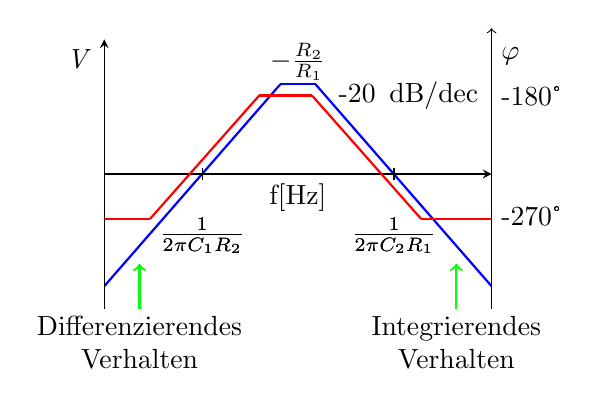
\begin{tikzpicture}[scale=1, transform shape]
    \begin{axis}[
        width=6.5cm, % Breite des Graphen
        height=5cm, % Höhe des Graphen
        xmin=0, xmax=11,
        ymin=-1.2, ymax=1.2,
        axis lines=center,
        axis on top=true,
        domain=0:10,
        clip mode=individual, % Verhindert das Abschneiden von Elementen
        xtick=\empty,
        ytick=\empty,
        ylabel style={xshift=-0.6cm},
        ylabel={\it V},
        xlabel={f[Hz]},
        xlabel style={at={(axis description cs:0.5,0.5)},anchor=north}
        ]
        \path[draw=none] (axis cs:-2, 0) rectangle (axis cs:13,1); \path[draw=none] (axis cs:-2, 0) rectangle (axis cs:13,1);


        \addplot+[mark=none, thick, blue] coordinates {(0,-1) (5,0.8)};
        \addplot+[mark=none, thick, blue] coordinates {(5,0.8) (6,0.8)};
        \addplot+[mark=none, thick, blue] coordinates {(6,0.8) (11,-1)};
        \node[anchor=north] at (axis cs:5.5,1.25) {$-\frac{R_2}{R_1}$};
        \addplot+[only marks, mark=|, black] coordinates {(2.78,0)} node[anchor=south] at (axis cs:2.78,-0.8) {$\frac{1}{2 \pi C_1 R_2}$};
        \addplot+[only marks, mark=|, black] coordinates {(8.23,0)} node[anchor=south] at (axis cs:8.23,-0.8) {$\frac{1}{2\pi C_2 R_1}$};
        \node[anchor=east] at (axis cs:10.9,0.7) {-20\, \text{dB/dec}};
        \addplot+[only marks, mark=|, black] coordinates {(2.78,0)} node[anchor=south] at (axis cs:2.78,-0.8) {$\frac{1}{2 \pi C_1 R_2}$};
        \addplot+[only marks, mark=|, black] coordinates {(8.23,0)} node[anchor=south] at (axis cs:8.23,-0.8) {$\frac{1}{2\pi C_2 R_1}$};
        \draw[->, thick, green] (axis cs:1,-1.2) -- (axis cs:1,-0.8);
        \node[align=center, black] at (axis cs:1,-1.5) {Differenzierendes\\ Verhalten};
        
        \draw[->, thick, green] (axis cs:10,-1.2) -- (axis cs:10,-0.8);
        \node[align=center, black] at (axis cs:10,-1.5) {Integrierendes\\ Verhalten};
        
    \end{axis}
    
    \begin{axis}[
        width=6.5cm, % Breite des Graphen
        height=5cm, % Höhe des Graphen
        xmin=0, xmax=11,
        ymin=0, ymax=240, 
        axis y line*=right,
        axis x line=none,
        ylabel={$\varphi$},
        ylabel style={rotate=270, anchor=west, yshift=1.5cm},
        xtick=\empty,
        ytick=\empty,
        clip mode=individual, % Verhindert das Abschneiden von Elementen
        after end axis/.code={
            \draw[->] (axis cs:11,240) -- (axis cs:11,250);
        }
        ]
        \addplot+[mark=none, thick, red] coordinates {(0,80) (1.3,80)};
        \addplot+[mark=none, thick, red] coordinates {(1.3,80) (4.4,190)};
        \addplot+[mark=none, thick, red] coordinates {(4.4,190) (5.9,190)};
        \addplot+[mark=none, thick, red] coordinates {(5.9,190) (9,80)};
        \addplot+[mark=none, thick, red] coordinates {(9,80) (11,80)};
        \node[anchor=west] at (axis cs:11,82.5) {-270°};
        \node[anchor=west] at (axis cs:11,190) {-180°};
       
    \end{axis}

    
    \end{tikzpicture}
    \begin{multline*}
        U_A = - \frac{R_2}{R_1} U_{\textnormal{E}}(t) \\
        - \int_0^t \frac{1}{R_1 C_1} U_{\textnormal{E}}(t) \, dt 
        - R_2 C_2\frac{dU_{\textnormal{E}}(t)}{dt}
    \end{multline*}
    \end{center} 
    & 
    \textbf{Differenzierer}\newline
    \begin{itemize}
        \item Nimmt eine Integration des Eingangssignals vor
        \item Wird als aktives Hochpassfilter verwendet (zeigt in der Realität meist Bandpassverhalten, wie hier dargestellt)
    \end{itemize}
    \\
    \hline
\end{tabular}
\end{table}






\newpage
    \begin{table}[ht]
        \begin{tabular}{|m{0.285\textwidth}|m{0.395\textwidth}|m{0.33\textwidth}|}
            \hline 
    Schaltung & Frequenzgang und Gleichung & Erläuterung und Eigenschaften \\ % Neue Zeile mit Text
    \hline
    \begin{circuitikz}[scale=0.7, transform shape]
    \ctikzset{
          resistors/scale=0.8,              
          tripoles/en amp/height=1.4, % Höhe des OPV             
          tripoles/en amp/width=1.4,   % Breite des OPV
         diodes/scale=0.8,
         tripoles/en amp/input height=0.45
     }
     \draw
     (0,0) node[en amp] (opamp) {}
     (opamp.-) to[R, l_=$R_1$, *-] ++(-1.2,0) to[short, o-] ++(0,0) node[left] {$U_E$}
     (opamp.+) -- ++(0,0) node[ground] {}
     (opamp.-) |- ++(0,1.5) to[D, l^=$D_1$] ++(2,0) -| (opamp.out)
     (opamp.out) to[short, *-o] ++(0.2,0) node[right] {$U_{A}$};
 \end{circuitikz}
    &
    \begin{center}
    \[
    U_{\textnormal{A}} =-U_{\textnormal{T}}\cdot \ln{\left(\frac{U_{\textnormal{E}}}{R_1\cdot I_S}\right)}
    \]
        \[
            U_{\textnormal{T}} = \frac{k_{\textnormal{B}} \cdot T}{e}
            \]
            
            \(e = \text{Elementarladung}\)
            
            \(k_{\textnormal{B}} = \text{Boltzmannkonstante}\)
            
            \(I_{\textnormal{s}} = \text{Sperrstrom der Diode}\)
    \end{center} 
    & 
    \textbf{Logarithmierer}\newline
    Bildet den natürlichen Logarithmus des Eingangssignals
    \\
    \hline
    \begin{circuitikz}[scale=0.7, transform shape]
    \ctikzset{
          resistors/scale=0.8,              
          tripoles/en amp/height=1.4, % Höhe des OPV            
          tripoles/en amp/width=1.4,   % Breite des OPV
         diodes/scale=0.8,
         tripoles/en amp/input height=0.45
     }
     \draw
     (0,0) node[en amp] (opamp) {}
     (opamp.-) to[D, l_=$D_1$, invert, *-] ++(-1.2,0) to[short, o-] ++(0,0) node[left] {$U_E$}
     (opamp.+) -- ++(0,0) node[ground] {}
     (opamp.-) |- ++(0,1.5) to[R, l^=$R_1$] ++(2,0) -| (opamp.out)
     (opamp.out) to[short, *-o] ++(0.2,0) node[right] {$U_{A}$};
 \end{circuitikz}
    &
    \begin{center}
    \[
    U_{\textnormal{A}} =-R_1\cdot I_{\textnormal{S}} \cdot e^{\frac{U_{\textnormal{E}}}{U_{\textnormal{T}}}}
    \]
    \end{center} 
    & 
    \textbf{Potenzierer}\newline
    Besitzt einen e-funktionalen Zusammenhang zwischen Ein- und Ausgangsspannung
    \\
    \hline
    \begin{circuitikz}[scale=0.6, transform shape]
    \ctikzset{
         resistors/scale=0.8,              
         tripoles/en amp/height=1.4, % Höhe des OPV             
         tripoles/en amp/width=1.4   % Breite des OPV
    }
    \draw 
    % Erster OPV mit input height=-0.45
    (2,-4.5) node[en amp, noinv input down] (opamp1) {}
    (opamp1.+) --++ (-0.5,0) node[ocirc, label=left:$U_{E2}$] (eingang1) {};
    
   \draw (2,0) node[en amp, noinv input up] (opamp2) {}
    (opamp2.+) --++ (-0.5,0) node[ocirc, label=left:$U_{E1}$] (eingang2) {}
    (opamp1.-)  to[R=$R_g$] (opamp2.-);

   % Dritter OPV mit angepasstem Eingangsabstand
    \ctikzset{tripoles/en amp/input height=0.55} % Anpassung nur für diesen OPV
    \draw (6,-2.25) node[en amp] (opamp3) {}
    (opamp3.-) -- ++(-0.5,0) to[R=$R_1$] ++(-1.5,0) to[R=$R_2$] ++(-2,0) node[circ]{}
    (opamp3.+) -- ++(-0.5,0) to[R=$R_3$] ++(-1.5,0) to[R=$R_4$] ++(-2,0) node[circ]{}
    (opamp2.out) -- ++(0,-1.72) node[circ]{}
    (opamp1.out) -- ++(0,1.72) node[circ]{}
    (opamp3.out) node[circ, label=below:{$U_A$}]{} -- ++(0, 2) to[R=$R_5$] ++(-2,0) -- ++(0, -1.45)node[circ]{};

\end{circuitikz}
     &
         \begin{center}
   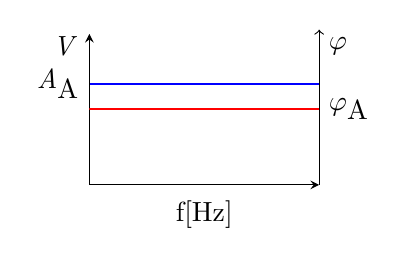
\begin{tikzpicture}[scale=1, transform shape]
    \begin{axis}[
        width=4.5cm, % Breite des Graphen
        height=3.5cm, % Höhe des Graphen
        xmin=0, xmax=10,
        ymin=0, ymax=120,
        axis lines=left,
        axis on top=true,
        domain=0:10,
        xtick=\empty,
        ytick=\empty,
        ylabel style={rotate=270, anchor=east, yshift=0.8cm}, % Position der Beschriftung oben links, horizontal
         ylabel={\it V}, % Hier die gewünschte Beschriftung einfügen
        xlabel={f[Hz]},
        clip mode=individual % Verhindert das Abschneiden von Elementen
        ]
        \addplot+[mark=none, thick, blue] coordinates {(0,80) (10,80)};
        % Adding the left-side label
        \node[anchor=east] at (axis cs:0,80) {$\mathit{A}_{\textnormal{A}}$};
    \end{axis}
    \begin{axis}[
        width=4.5cm, % Breite des Graphen
        height=3.5cm, % Höhe des Graphen
        xmin=0, xmax=10,
        ymin=-180, ymax=180,
        axis y line*=right,
        axis x line=none,
        ytick=\empty,
        ylabel={$\varphi$},
        ylabel style={rotate=270, anchor=west, yshift=0.8cm},
        clip mode=individual, % Verhindert das Abschneiden von Elementen
        after end axis/.code={
            \draw[->] (axis cs:10,180) -- (axis cs:10,190);
        }
        ]
        \addplot+[mark=none, thick, red] coordinates {(0,0) (10,0)};
        \node[anchor=west] at (axis cs:10,0) {$\varphi_{\textnormal{A}}$};
    \end{axis}
    \end{tikzpicture}
\end{center}

\vspace{1ex}
\[
\mathit{a_i} : \text{Amplitude Eingangsspannung i}
\]
\[
\mathit{\varphi_i} : \text{Phase Eingangsspannung i}
\]
\[
\mathit{A}_{A} = \sqrt{a_1^2 + a_2^2 + 2a_1a_2 \cos(\varphi_1 - \varphi_2)}
\]
\[
\mathit{\tan}(\varphi_A) = \frac{a_1 \mathit{\sin}(\varphi_1) + a_2 \mathit{\sin}(\varphi_2)}{a_1 \mathit{\cos}(\varphi_1) + a_2 \mathit{\cos}(\varphi_2)}
\]
\[
    \text{Wenn} : R_2 = R_4 = R
\]
\[
    U_{\textnormal{A}} = (1+ \frac{2R} {R_{\textnormal{g}}}) \cdot \frac{R_3} {R_2} (U_{\textnormal{E2}}-U_{\textnormal{E1}})
\]
     & 
     \textbf{Instrumentenverstärker}\newline
    Differenzverstärker mit hoher Eingangsimpedanz und hoher Gleichtaktunterdrückung  

    \\
    \hline
    \end{tabular}
\end{table}


            %\label{OPV Schaltungen Tabelle}
            %\caption{Tabelle mit ausgewählten Operationsverstärkerschaltungen}
        \end{block}
        %\label{fig:Frequenzgang OPVs}
    }	
   \b{\frametitle{Prinzip der Gegenkopplung - Lösung des Beispielproblems (3)}
    \begin{columns}
        \column[c]{0.3\textwidth}
            \begin{center}
                    \begin{circuitikz}[scale=0.8, transform shape]
        \ctikzset{tripoles/en amp/input height=-0.45,
        }
        \draw (0,0) node[en amp](E){};
        \node at ($(E) + (-1.2, 1.5)$) {\textbf{\LARGE D}}; % Label für den OPV im dritten Bild
        \draw (E.out) node[circ]{} -- ++(0.2,0) node[ocirc, right]{};
        \draw (E.-) -- ++(0, -1.3) node[circ] {} to[R, l=$R_2$] ++(2.38,0) -- ++(0,1.8);
        \draw (E.-) -- ++(0, -1.6) to[R, l_=$R_1$] ++(0, -1.2) -- ++(0,-0.2) -- ++(-0.2, 0) -- ++(0.4,0);
        \draw (E.+) node[circ]{} node[left]{};     
       
        % Spannungspfeil
        \draw[-{Triangle[width=3pt,length=4pt]}, color=spannung] ($(E.+) + (0, -0.1)$) -- ($(E.-) + (0, 0.1)$) node[midway, xshift=-32] {$U_{Diff}=0\,\text{V}$};
        \draw[-{Triangle[width=3pt,length=4pt]}, color=spannung] ($(E.out) + (0.26, -0.1)$) -- ($(E.out) + (0.26, -3.45)$) node[midway, xshift=10] {$U_A$};
        \draw[black] ($(E.out) + (0.26, -3.5)$) -- ++(-0.2, 0) -- ++(0.4,0);
        \draw[-{Triangle[width=3pt,length=4pt]}, color=spannung] (0.7,-2.1)-- ++(-1.5,0) node[midway, yshift=-8] {$U_{R2}$};
        \draw[-{Triangle[width=3pt,length=4pt]}, color=spannung] (-0.9,-2)-- ++(0,-1.5) node[midway, xshift=10] {$U_{R1}$};


        
        \node[red] at (0.9,-1.8) {\tikz \draw[red, -{Triangle[width=3pt,length=4pt]}] (0,0) -- (-0.01,0);};
        \node[above, color=red] at (0.9,-1.8)  {$I_{R2}$};

        \node[red] at ($(E.-)+(0,-1.5)$) {\tikz \draw[red, -{Triangle[width=3pt,length=4pt]}] (0,0) -- (0,-0.01);};
        \node[left, color=red] at ($(E.-)+(0,-1.4)$)  {$I_{R1}$};
      
        % Strompfeil oberhalb von R1
        %\draw[->, thick, red] (-1.19,-1) -- ++(0, -0.01);
        %\node[red] at (-1.5, -1) {$I_{R_1}$};
    \end{circuitikz}
                Finale Verstärkerschaltung mit Rückführung
                \label{fig:Verschaltung des Verstärkers2}             
            \end{center}        
        \column[c]{0.6\textwidth}
        Annahme: $U_{\textnormal{Diff}}$~=~0
        \onslide<1->{
            \begin{equation}
                U_{A} = U_{R1} + U_{R2} = U_{E} + I_{R2} \cdot R_2 
            \end{equation}}
        \onslide<2->{
            \begin{equation}
                U_{A} = U_{E} + \frac{U_{E}}{R_1} \cdot R_2 
            \end{equation}}
        \onslide<3->{
            \begin{equation}
                \frac{U_{A}}{U_{E}} = \underbrace{(1+\frac{R_2}{R_1})}_{V_{Gain}}
            \end{equation}}
        \onslide<3->{
        
        Weitere OPV-Grundschaltungen sind Skript zu finden.}
        \end{columns} 
    }
 \end{frame}

%Folie Nichtinvertierender Verstärker
\begin{frame}
    \b{
    \frametitle{Nichtinvertierender Verstärker neu}
    \begin{columns}
        \column{0.48\textwidth}
        \centering
        \begin{figure}
    \centering

    \begin{subfigure}{\linewidth}
        \centering
        \resizebox{0.6\linewidth}{!}{\begin{circuitikz}[scale=0.7, transform shape]
    \ctikzset{
         resistors/scale=0.8,              
         tripoles/en amp/height=1.4, % Höhe des OPV             
         tripoles/en amp/width=1.4,   % Breite des OPV
         tripoles/en amp/input height=-0.45
    }
    \vspace{1ex}
    \draw (2,-0.1) node[en amp] (opamp) {}
    (opamp.+) --++ (-0.5,0) node[ocirc, label=left:$U_E$] (eingang) {} 
    (opamp.out) --++ (0.5,0) node[ocirc, label=right:$U_A$] {}
    (opamp.-) -- ++(0, -1.5) to[R, l=$R_1$] ++(0, -1) node[ground] {}
    (opamp.out) node[circ] {} -- ++(0,-1.5) to[R, l=$R_2$] ++(-1.95,0) node[circ] (feedback) {};
\end{circuitikz}

}
        \caption{Schaltung eines nichtinvertierenden Verstärkers}
    \end{subfigure}

    \vspace{0.5cm} 

    \begin{subfigure}{\linewidth}
        \centering
        \resizebox{0.6\linewidth}{!}{\begin{tikzpicture}[scale=1, transform shape]
    \begin{axis}[
    width=4.5cm, % Breite des Graphen
    height=3.5cm, % Höhe des Graphen
    xmin=0, xmax=10,
    ymin=0, ymax=120,
    axis lines=left,
    axis on top=true,
    domain=0:10,
    xtick=\empty,
    ytick=\empty,
    ylabel style={rotate=270, anchor=east, yshift=1cm}, % Position der Beschriftung oben links, horizontal
     ylabel={\it V}, % Hier die gewünschte Beschriftung einfügen
    xlabel={f[Hz]},
    clip mode=individual % Verhindert das Abschneiden von Elementen
    ]
    \path[draw=none] (axis cs:-4, 0) rectangle (axis cs:16.6,120);
    
    
    \coordinate (xaxis) at (axis description cs:15.5,0); % Verwendet die relative Positionierung für x-Achse
    
    \addplot+[mark=none, thick, blue] coordinates {(0,80) (10,80)};
    % Adding the left-side label
    \node[anchor=east] at (axis cs:0,80) {$1 + \frac{R_2}{R_1}$};
    \end{axis}
    \begin{axis}[
    width=4.5cm, % Breite des Graphen
    height=3.5cm, % Höhe des Graphen
    xmin=0, xmax=10,
    ymin=-180, ymax=180,
    axis y line*=right,
    axis x line=none,
    ytick=\empty,
    ylabel={$\varphi$},
    ylabel style={rotate=270, anchor=west, yshift=0.8cm},
    clip mode=individual, % Verhindert das Abschneiden von Elementen
    after end axis/.code={
        \draw[->] (axis cs:10,180) -- (axis cs:10,190);
    }
    ]
    \addplot+[mark=none, thick, red] coordinates {(0,0) (10,0)};
    \node[anchor=west] at (axis cs:10,0) {$0^\circ$};
    \end{axis}
    \end{tikzpicture}}
        \caption{Frequenzgang eines nichtinvertierenden Verstärkers}
    \end{subfigure}

\end{figure}

        \column{0.48\textwidth}
        \begin{itemize}
            \item Gleichung:
            \[
            U_{\textnormal{A}} = \left(1+\frac{R_2}{R_1}\right) U_{\textnormal{E}}
            \]
            \item Phasengleiches Ausgangssignal
            \item Sehr hochohmiger Eingangswiderstand
            \item Niederohmiger Ausgangswiderstand
            \item Anwendungen: z.B. Impedanzwandler
        \end{itemize}
    \end{columns}
    }
\end{frame}


\begin{frame}
    \b{
    \frametitle{Nichtinvertierender Verstärker}
    \centering
    \begin{table}[ht]
    \label{tab:NichtinvertierenderVerstaerker}
    \begin{tabular}{|m{0.24\textwidth}|m{0.405\textwidth}|m{0.25\textwidth}|}
    \hline
    Schaltung & Frequenzgang und Gleichung & Erläuterung und Eigenschaften\\ % Neue Zeile mit Text
    \hline
    \vspace{0.5cm}
    \centering
    \begin{circuitikz}[scale=0.7, transform shape]
    \ctikzset{
         resistors/scale=0.8,              
         tripoles/en amp/height=1.4, % Höhe des OPV             
         tripoles/en amp/width=1.4,   % Breite des OPV
         tripoles/en amp/input height=-0.45
    }
    \vspace{1ex}
    \draw (2,-0.1) node[en amp] (opamp) {}
    (opamp.+) --++ (-0.5,0) node[ocirc, label=left:$U_E$] (eingang) {} 
    (opamp.out) --++ (0.5,0) node[ocirc, label=right:$U_A$] {}
    (opamp.-) -- ++(0, -1.5) to[R, l=$R_1$] ++(0, -1) node[ground] {}
    (opamp.out) node[circ] {} -- ++(0,-1.5) to[R, l=$R_2$] ++(-1.95,0) node[circ] (feedback) {};
\end{circuitikz}

 & \begin{tikzpicture}[scale=1, transform shape]
    \begin{axis}[
    width=4.5cm, % Breite des Graphen
    height=3.5cm, % Höhe des Graphen
    xmin=0, xmax=10,
    ymin=0, ymax=120,
    axis lines=left,
    axis on top=true,
    domain=0:10,
    xtick=\empty,
    ytick=\empty,
    ylabel style={rotate=270, anchor=east, yshift=1cm}, % Position der Beschriftung oben links, horizontal
     ylabel={\it V}, % Hier die gewünschte Beschriftung einfügen
    xlabel={f[Hz]},
    clip mode=individual % Verhindert das Abschneiden von Elementen
    ]
    \path[draw=none] (axis cs:-4, 0) rectangle (axis cs:16.6,120);
    
    
    \coordinate (xaxis) at (axis description cs:15.5,0); % Verwendet die relative Positionierung für x-Achse
    
    \addplot+[mark=none, thick, blue] coordinates {(0,80) (10,80)};
    % Adding the left-side label
    \node[anchor=east] at (axis cs:0,80) {$1 + \frac{R_2}{R_1}$};
    \end{axis}
    \begin{axis}[
    width=4.5cm, % Breite des Graphen
    height=3.5cm, % Höhe des Graphen
    xmin=0, xmax=10,
    ymin=-180, ymax=180,
    axis y line*=right,
    axis x line=none,
    ytick=\empty,
    ylabel={$\varphi$},
    ylabel style={rotate=270, anchor=west, yshift=0.8cm},
    clip mode=individual, % Verhindert das Abschneiden von Elementen
    after end axis/.code={
        \draw[->] (axis cs:10,180) -- (axis cs:10,190);
    }
    ]
    \addplot+[mark=none, thick, red] coordinates {(0,0) (10,0)};
    \node[anchor=west] at (axis cs:10,0) {$0^\circ$};
    \end{axis}
    \end{tikzpicture}
\vspace{1ex}
\[
U_{\textnormal{A}} = \left(1+\frac{R_2}{R_1}\right) U_{\textnormal{E}}
\]
    &
\begin{itemize}
    \item Phasengleiches Ausgangs-\linebreak signal
    \item Sehr hochohmiger Eingangswiderstand
    \item Niederohmiger Ausgangs-\linebreak widerstand
    \item Anwendungen: z.B. Impedanzwandler
\end{itemize} \\
    \hline
    \end{tabular}
    \end{table}
    }
\end{frame}


%Folie Invertierender Verstärker
\begin{frame}
    \b{
    \frametitle{Invertierender Verstärker}
    \centering
    \begin{table}[ht]
    \label{tab:InvertierenderVerstaerker}
    \begin{tabular}{|m{0.24\textwidth}|m{0.405\textwidth}|m{0.25\textwidth}|}
    \hline
    Schaltung & Frequenzgang und Gleichung & Erläuterung und Eigenschaften\\ % Neue Zeile mit Text
    \hline
    \vspace{0.5cm}
    \centering
    \begin{circuitikz}[scale=0.7, transform shape]
    \ctikzset{
          resistors/scale=0.8,              
          tripoles/en amp/height=1.4, % Höhe des OPV             
          tripoles/en amp/width=1.4,   % Breite des OPV
         tripoles/en amp/input height=0.45
     }
     \draw
     (0,0) node[en amp] (opamp) {}
     (opamp.-) to[R, l_=$R_1$, *-] ++(-1.2,0) to[short, o-] ++(0,0) node[left] {$U_E$}
     (opamp.+) -- ++(0,0) node[ground] {}
     (opamp.-) |- ++(0,1) to[R, l=$R_2$] ++(1.9,0) -| (opamp.out)
     (opamp.out) to[short, *-o] ++(0.2,0) node[right] {$U_{A}$};
 \end{circuitikz}
     & 
    \begin{center}
        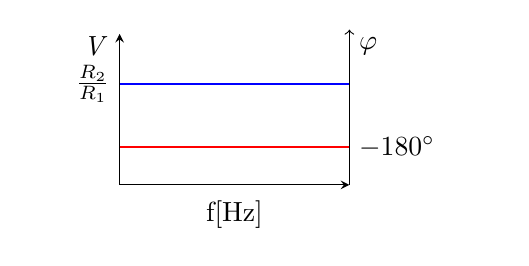
\begin{tikzpicture}[scale=1, transform shape]
    \begin{axis}[
        width=4.5cm, % Breite des Graphen
        height=3.5cm, % Höhe des Graphen
        xmin=0, xmax=10,
        ymin=0, ymax=120,
        axis lines=left,
        axis on top=true,
        domain=0:10,
        xtick=\empty,
        ytick=\empty,
        ylabel style={rotate=270, anchor=east, yshift=0.8cm},
         ylabel={\it V},
        xlabel={f[Hz]},
        clip mode=individual % Verhindert das Abschneiden von Elementen
        ]
        \path[draw=none] (axis cs:-4, 0) rectangle (axis cs:16.6,120);
    
        \addplot+[mark=none, thick, blue] coordinates {(0,80) (10,80)};
        % Adding the left-side label
        \node[anchor=east] at (axis cs:0,80) {$\frac{R_2}{R_1}$};
    \end{axis}
    \begin{axis}[
        width=4.5cm, % Breite des Graphen
        height=3.5cm, % Höhe des Graphen
        xmin=0, xmax=10,
        ymin=-180, ymax=180,
        axis y line*=right,
        axis x line=none,
        ytick=\empty,
        ylabel={$\varphi$},
        ylabel style={rotate=270, anchor=west, yshift=0.8cm},
        clip mode=individual, % Verhindert das Abschneiden von Elementen
        after end axis/.code={
            \draw[->] (axis cs:10,180) -- (axis cs:10,190);
        }
        ]
        \addplot+[mark=none, thick, red] coordinates {(0,-90) (10,-90)};
        \node[anchor=west] at (axis cs:10,-90) {$-180^\circ$};
    \end{axis}
    \end{tikzpicture}
\end{center}
\vspace{1ex}
\[
    U_{\textnormal{A}} = \frac{R_2}{R_1} U_{\textnormal{E}}
\]
    &
\begin{itemize}
    \item -180$^\circ$ Phasenverschiebung zwischen Ein- zu Ausgang
    \item $R_1$ bestimmt den Eingangswiderstand
    \item Niederohmiger Ausgangs-\linebreak widerstand
    \item Anwendungen: \linebreak z.B. Aktiver Spannungsteiler zum Messen hoher Spannungen, wenn $R_1 > R_2$
\end{itemize} \\
    \hline
    \end{tabular}
    \end{table}
    }
\end{frame}

\begin{frame}
    \b{
    \frametitle{Invertierender Verstärker neu}
    \begin{columns}
        \column{0.48\textwidth}
        \centering
        \begin{figure}
    \centering

    \begin{subfigure}{\linewidth}
        \centering
        \resizebox{0.6\linewidth}{!}{\begin{circuitikz}[scale=0.7, transform shape]
    \ctikzset{
          resistors/scale=0.8,              
          tripoles/en amp/height=1.4, % Höhe des OPV             
          tripoles/en amp/width=1.4,   % Breite des OPV
         tripoles/en amp/input height=0.45
     }
     \draw
     (0,0) node[en amp] (opamp) {}
     (opamp.-) to[R, l_=$R_1$, *-] ++(-1.2,0) to[short, o-] ++(0,0) node[left] {$U_E$}
     (opamp.+) -- ++(0,0) node[ground] {}
     (opamp.-) |- ++(0,1) to[R, l=$R_2$] ++(1.9,0) -| (opamp.out)
     (opamp.out) to[short, *-o] ++(0.2,0) node[right] {$U_{A}$};
 \end{circuitikz}}
        \caption{Schaltung eines invertierenden Verstärkers}
    \end{subfigure}

    \vspace{0.5cm} 

    \begin{subfigure}{\linewidth}
        \centering
        \resizebox{0.6\linewidth}{!}{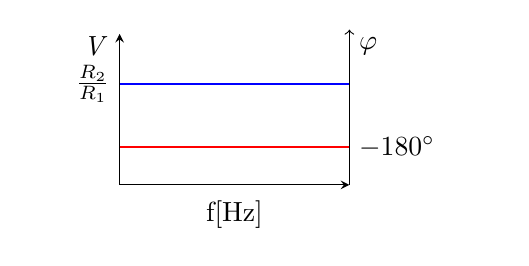
\begin{tikzpicture}[scale=1, transform shape]
    \begin{axis}[
        width=4.5cm, % Breite des Graphen
        height=3.5cm, % Höhe des Graphen
        xmin=0, xmax=10,
        ymin=0, ymax=120,
        axis lines=left,
        axis on top=true,
        domain=0:10,
        xtick=\empty,
        ytick=\empty,
        ylabel style={rotate=270, anchor=east, yshift=0.8cm},
         ylabel={\it V},
        xlabel={f[Hz]},
        clip mode=individual % Verhindert das Abschneiden von Elementen
        ]
        \path[draw=none] (axis cs:-4, 0) rectangle (axis cs:16.6,120);
    
        \addplot+[mark=none, thick, blue] coordinates {(0,80) (10,80)};
        % Adding the left-side label
        \node[anchor=east] at (axis cs:0,80) {$\frac{R_2}{R_1}$};
    \end{axis}
    \begin{axis}[
        width=4.5cm, % Breite des Graphen
        height=3.5cm, % Höhe des Graphen
        xmin=0, xmax=10,
        ymin=-180, ymax=180,
        axis y line*=right,
        axis x line=none,
        ytick=\empty,
        ylabel={$\varphi$},
        ylabel style={rotate=270, anchor=west, yshift=0.8cm},
        clip mode=individual, % Verhindert das Abschneiden von Elementen
        after end axis/.code={
            \draw[->] (axis cs:10,180) -- (axis cs:10,190);
        }
        ]
        \addplot+[mark=none, thick, red] coordinates {(0,-90) (10,-90)};
        \node[anchor=west] at (axis cs:10,-90) {$-180^\circ$};
    \end{axis}
    \end{tikzpicture}}
        \caption{Frequenzgang eines invertierenden Verstärkers}
    \end{subfigure}

\end{figure}

        \column{0.48\textwidth}
        \begin{itemize}
            \item Gleichung:
           \[
    U_{\textnormal{A}} = \frac{R_2}{R_1} U_{\textnormal{E}}
            \]
    \item -180$^\circ$ Phasenverschiebung zwischen Ein- zu Ausgang
    \item $R_1$ bestimmt den Eingangswiderstand
    \item Niederohmiger Ausgangswiderstand
    \item Anwendungen: z.B. Aktiver Spannungsteiler zum Messen hoher Spannungen, wenn $R_1 > R_2$
        \end{itemize}
    \end{columns}
    }
\end{frame}

%Folie Komparator
\begin{frame}
    \b{
    \frametitle{Komparator}
    \centering
    \begin{table}[ht]
    \label{tab:Komparator}
    \begin{tabular}{|m{0.24\textwidth}|m{0.405\textwidth}|m{0.25\textwidth}|}
    \hline
    Schaltung & Frequenzgang und Gleichung & Erläuterung und Eigenschaften\\ % Neue Zeile mit Text
    \hline
    \vspace{0.5cm}
    \centering
    \begin{circuitikz}[scale=0.7, transform shape]
    \ctikzset{
          resistors/scale=0.8,              
          tripoles/en amp/height=1.4, % Höhe des OPV             
          tripoles/en amp/width=1.4,   % Breite des OPV
         tripoles/en amp/input height=0.45
     }
     \draw
     (0,0) node[en amp] (opamp) {}
     (opamp.-)  to[short, o-] ++(0,0) node[left] {$U_{E-}$}
      (opamp.+) to[short, o-] ++(0,0) node[left] {$U_{E+}$}
     (opamp.out) to[short, -o] ++(0,0) node[right] {$U_{A}$};
 \end{circuitikz}
    & 
    \begin{center}
               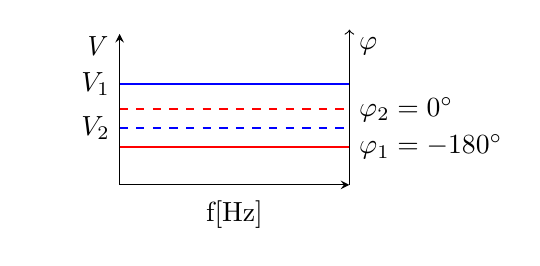
\begin{tikzpicture}[scale=1, transform shape]
    \begin{axis}[
        width=4.5cm, % Breite des Graphen
        height=3.5cm, % Höhe des Graphen
        xmin=0, xmax=10,
        ymin=0, ymax=120,
        axis lines=left,
        axis on top=true,
        domain=0:10,
        xtick=\empty,
        ytick=\empty,
        ylabel style={rotate=270, anchor=east, yshift=0.8cm},
         ylabel={\it V},
        xlabel={f[Hz]},
        clip mode=individual % Verhindert das Abschneiden von Elementen
        ]
        \path[draw=none] (axis cs:-4, 0) rectangle (axis cs:16.6,120);

        \addplot+[mark=none, thick, blue] coordinates {(0,80) (10,80)};
        \addplot+[mark=none, thick, blue, dashed] coordinates {(0,45) (10,45)};
        % Adding the left-side label
        \node[anchor=east] at (axis cs:0,80) {$V_1$};
        \node[anchor=east] at (axis cs:0,45) {$V_2$};
    \end{axis}
    \begin{axis}[
        width=4.5cm, % Breite des Graphen
        height=3.5cm, % Höhe des Graphen
        xmin=0, xmax=10,
        ymin=-180, ymax=180,
        axis y line*=right,
        axis x line=none,
        ytick=\empty,
        ylabel={$\varphi$},
        ylabel style={rotate=270, anchor=west, yshift=0.8cm},
        clip mode=individual, % Verhindert das Abschneiden von Elementen
        after end axis/.code={
            \draw[->] (axis cs:10,180) -- (axis cs:10,190);
        }
        ]
        \addplot+[mark=none, thick, red, dashed] coordinates {(0,0) (10,0)};
        \addplot+[mark=none, thick, red] coordinates {(0,-90) (10,-90)};
        \node[anchor=west] at (axis cs:10,0) {$\varphi_2 = 0^\circ$};
        \node[anchor=west] at (axis cs:10,-90) {$\varphi_1 = -180^\circ$};
    \end{axis}
    \end{tikzpicture}
\[
V_1: U_{\textnormal{E+}} > U_{\textnormal{E-}} \Rightarrow U_{\textnormal{A}} \approx +U_{\textnormal{B}}
\]
\[
V_2: U_{\textnormal{E+}} < U_{\textnormal{E-}} \Rightarrow U_{\textnormal{A}} \approx -U_{\textnormal{B}}
\]
\end{center}
    &\textbf{Komparator}\newline
    Einsatz in Zweipunktreglern und Analog-Digital-Wandlern \\
    \hline
    \end{tabular}
    \end{table}
    }
\end{frame}

\begin{frame}
    \b{
    \frametitle{Komparator neu}
    \begin{columns}
        \column{0.48\textwidth}
        \centering
        \begin{figure}
    \centering

    \begin{subfigure}{\linewidth}
        \centering
        \resizebox{0.6\linewidth}{!}{\begin{circuitikz}[scale=0.7, transform shape]
    \ctikzset{
          resistors/scale=0.8,              
          tripoles/en amp/height=1.4, % Höhe des OPV             
          tripoles/en amp/width=1.4,   % Breite des OPV
         tripoles/en amp/input height=0.45
     }
     \draw
     (0,0) node[en amp] (opamp) {}
     (opamp.-)  to[short, o-] ++(0,0) node[left] {$U_{E-}$}
      (opamp.+) to[short, o-] ++(0,0) node[left] {$U_{E+}$}
     (opamp.out) to[short, -o] ++(0,0) node[right] {$U_{A}$};
 \end{circuitikz}}
        \caption{Schaltung eines Komparators}
    \end{subfigure}

    \vspace{0.5cm} 

    \begin{subfigure}{\linewidth}
        \centering
        \resizebox{0.6\linewidth}{!}{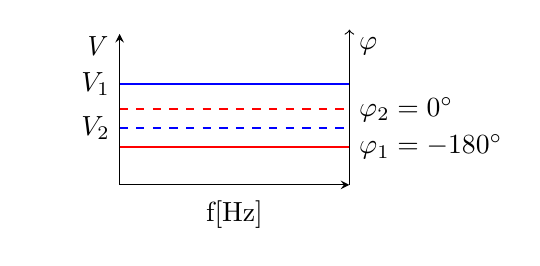
\begin{tikzpicture}[scale=1, transform shape]
    \begin{axis}[
        width=4.5cm, % Breite des Graphen
        height=3.5cm, % Höhe des Graphen
        xmin=0, xmax=10,
        ymin=0, ymax=120,
        axis lines=left,
        axis on top=true,
        domain=0:10,
        xtick=\empty,
        ytick=\empty,
        ylabel style={rotate=270, anchor=east, yshift=0.8cm},
         ylabel={\it V},
        xlabel={f[Hz]},
        clip mode=individual % Verhindert das Abschneiden von Elementen
        ]
        \path[draw=none] (axis cs:-4, 0) rectangle (axis cs:16.6,120);

        \addplot+[mark=none, thick, blue] coordinates {(0,80) (10,80)};
        \addplot+[mark=none, thick, blue, dashed] coordinates {(0,45) (10,45)};
        % Adding the left-side label
        \node[anchor=east] at (axis cs:0,80) {$V_1$};
        \node[anchor=east] at (axis cs:0,45) {$V_2$};
    \end{axis}
    \begin{axis}[
        width=4.5cm, % Breite des Graphen
        height=3.5cm, % Höhe des Graphen
        xmin=0, xmax=10,
        ymin=-180, ymax=180,
        axis y line*=right,
        axis x line=none,
        ytick=\empty,
        ylabel={$\varphi$},
        ylabel style={rotate=270, anchor=west, yshift=0.8cm},
        clip mode=individual, % Verhindert das Abschneiden von Elementen
        after end axis/.code={
            \draw[->] (axis cs:10,180) -- (axis cs:10,190);
        }
        ]
        \addplot+[mark=none, thick, red, dashed] coordinates {(0,0) (10,0)};
        \addplot+[mark=none, thick, red] coordinates {(0,-90) (10,-90)};
        \node[anchor=west] at (axis cs:10,0) {$\varphi_2 = 0^\circ$};
        \node[anchor=west] at (axis cs:10,-90) {$\varphi_1 = -180^\circ$};
    \end{axis}
    \end{tikzpicture}}
        \caption{Frequenzgang eines Komparators}
    \end{subfigure}

\end{figure}

        \column{0.48\textwidth}
        \begin{itemize}
            \item Gleichung:
          \[
V_1: U_{\textnormal{E+}} > U_{\textnormal{E-}} \Rightarrow U_{\textnormal{A}} \approx +U_{\textnormal{B}}
\]
\[
V_2: U_{\textnormal{E+}} < U_{\textnormal{E-}} \Rightarrow U_{\textnormal{A}} \approx -U_{\textnormal{B}}
\]
    \item Einsatz in Zweipunktreglern und Analog-Digital-Wandlern
        \end{itemize}
    \end{columns}
    }
\end{frame}

%Folie Summierer

\begin{frame}
    \b{
    \frametitle{Summierer}
    \centering
    \begin{table}[ht]
    \label{tab:Summierer}
    \begin{tabular}{|m{0.24\textwidth}|m{0.405\textwidth}|m{0.25\textwidth}|}
    \hline
    Schaltung & Frequenzgang und Gleichung & Erläuterung und Eigenschaften\\ % Neue Zeile mit Text
    \hline
    \vspace{0.5cm}
    \centering
    \begin{circuitikz}[scale=0.7, transform shape]
    \ctikzset{
        resistors/scale=0.8,              
        tripoles/en amp/height=1.4, % Höhe des OPV             
        tripoles/en amp/width=1.4,   % Breite des OPV
        tripoles/en amp/input height=0.45
    }
    \draw
    (0,0) node[en amp] (opamp) {}
    % R2 mit korrigiertem Strompfeil
    (opamp.-) -- ++(-0.4,0) node[circ] {} to[R, l_=$R_2$] ++(-1.5,0) node[ocirc] (R2left) {}
    % R1 mit korrigiertem Strompfeil
    (opamp.-) -- ++(-0.4,0) --++(0,1) to[R, l_=$R_1$] ++(-1.5,0) node[ocirc] (R1left) {}
    % Erdung
    (opamp.+) -- ++(0,0) node[ground] {}
    % Ausgang
    (opamp.out) to[short, *-o] ++(0,0) node[right] {$U_{A}$}
    % R3 mit Strompfeil
    (opamp.out) -- ++(0,1.5) to[R, l_=$R_3$] ++(-2,0) -- ++(0,-1.05) node[circ] {}
    % Spannungen U_E1 und U_E2 an den Knoten links von R1 und R2
    (R1left) node[left] {$U_{E1}$}
    (R2left) node[left] {$U_{E2}$};
\end{circuitikz}

    &
    \begin{center}
    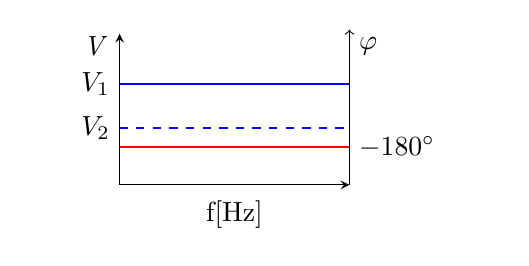
\begin{tikzpicture}[scale=1, transform shape]
    \begin{axis}[
        width=4.5cm, % Breite des Graphen
        height=3.5cm, % Höhe des Graphen
        xmin=0, xmax=10,
        ymin=0, ymax=120,
        axis lines=left,
        axis on top=true,
        domain=0:10,
        xtick=\empty,
        ytick=\empty,
        ylabel style={rotate=270, anchor=east, yshift=0.8cm},
         ylabel={\it V},
        xlabel={f[Hz]},
        clip mode=individual % Verhindert das Abschneiden von Elementen
        ]
        \addplot+[mark=none, thick, blue] coordinates {(0,80) (10,80)};
        \addplot+[mark=none, thick, blue, dashed] coordinates {(0,45) (10,45)};
    
        % Adding the left-side label
        \node[anchor=east] at (axis cs:0,80) {$V_1$};
        \node[anchor=east] at (axis cs:0,45) {$V_2$};
    \end{axis}
    \begin{axis}[
        width=4.5cm, % Breite des Graphen
        height=3.5cm, % Höhe des Graphen
        xmin=0, xmax=10,
        ymin=-180, ymax=180,
        axis y line*=right,
        axis x line=none,
        ytick=\empty,
        ylabel={$\varphi$},
        ylabel style={rotate=270, anchor=west, yshift=0.8cm},
        clip mode=individual, % Verhindert das Abschneiden von Elementen
        after end axis/.code={
            \draw[->] (axis cs:10,180) -- (axis cs:10,190);
        }
        ]
        \path[draw=none] (axis cs:-4, 0) rectangle (axis cs:16.6,120);
        \addplot+[mark=none, thick, red] coordinates {(0,-90) (10,-90)};
        \node[anchor=west] at (axis cs:10,-90) {$-180^\circ$};
    \end{axis}
    \end{tikzpicture}
\end{center}
\vspace{1ex}
\[
\begin{aligned}
    U_{\textnormal{A}} = \underbrace{\frac{R_3} {R_1}}_{V_1} \cdot U_{\textnormal{E1}} + \underbrace{\frac{R_3} {R_2}}_{V_2} \cdot U_{\textnormal{E2}}
\end{aligned}
\]
    & 
    Der Summierer basiert auf dem invertierenden Verstärker und findet Verwendung in Analogrechnern und beim Mischen von Spannungssignalen \\
    \hline
    \end{tabular}
    \end{table}
    }
\end{frame}

\begin{frame}
    \b{
    \frametitle{Summierer neu}
    \begin{columns}
        \column{0.48\textwidth}
        \centering
        \begin{figure}
    \centering

    \begin{subfigure}{\linewidth}
        \centering
        \resizebox{0.6\linewidth}{!}{\begin{circuitikz}[scale=0.7, transform shape]
    \ctikzset{
        resistors/scale=0.8,              
        tripoles/en amp/height=1.4, % Höhe des OPV             
        tripoles/en amp/width=1.4,   % Breite des OPV
        tripoles/en amp/input height=0.45
    }
    \draw
    (0,0) node[en amp] (opamp) {}
    % R2 mit korrigiertem Strompfeil
    (opamp.-) -- ++(-0.4,0) node[circ] {} to[R, l_=$R_2$] ++(-1.5,0) node[ocirc] (R2left) {}
    % R1 mit korrigiertem Strompfeil
    (opamp.-) -- ++(-0.4,0) --++(0,1) to[R, l_=$R_1$] ++(-1.5,0) node[ocirc] (R1left) {}
    % Erdung
    (opamp.+) -- ++(0,0) node[ground] {}
    % Ausgang
    (opamp.out) to[short, *-o] ++(0,0) node[right] {$U_{A}$}
    % R3 mit Strompfeil
    (opamp.out) -- ++(0,1.5) to[R, l_=$R_3$] ++(-2,0) -- ++(0,-1.05) node[circ] {}
    % Spannungen U_E1 und U_E2 an den Knoten links von R1 und R2
    (R1left) node[left] {$U_{E1}$}
    (R2left) node[left] {$U_{E2}$};
\end{circuitikz}}
        \caption{Schaltung eines Summierers}
    \end{subfigure}

    \vspace{0.5cm} 

    \begin{subfigure}{\linewidth}
        \centering
        \resizebox{0.6\linewidth}{!}{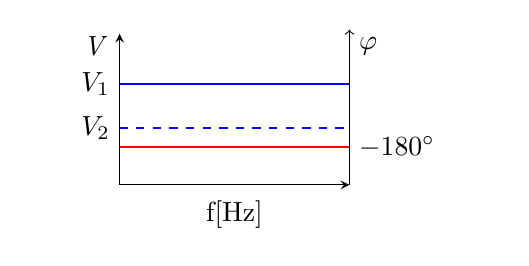
\begin{tikzpicture}[scale=1, transform shape]
    \begin{axis}[
        width=4.5cm, % Breite des Graphen
        height=3.5cm, % Höhe des Graphen
        xmin=0, xmax=10,
        ymin=0, ymax=120,
        axis lines=left,
        axis on top=true,
        domain=0:10,
        xtick=\empty,
        ytick=\empty,
        ylabel style={rotate=270, anchor=east, yshift=0.8cm},
         ylabel={\it V},
        xlabel={f[Hz]},
        clip mode=individual % Verhindert das Abschneiden von Elementen
        ]
        \addplot+[mark=none, thick, blue] coordinates {(0,80) (10,80)};
        \addplot+[mark=none, thick, blue, dashed] coordinates {(0,45) (10,45)};
    
        % Adding the left-side label
        \node[anchor=east] at (axis cs:0,80) {$V_1$};
        \node[anchor=east] at (axis cs:0,45) {$V_2$};
    \end{axis}
    \begin{axis}[
        width=4.5cm, % Breite des Graphen
        height=3.5cm, % Höhe des Graphen
        xmin=0, xmax=10,
        ymin=-180, ymax=180,
        axis y line*=right,
        axis x line=none,
        ytick=\empty,
        ylabel={$\varphi$},
        ylabel style={rotate=270, anchor=west, yshift=0.8cm},
        clip mode=individual, % Verhindert das Abschneiden von Elementen
        after end axis/.code={
            \draw[->] (axis cs:10,180) -- (axis cs:10,190);
        }
        ]
        \path[draw=none] (axis cs:-4, 0) rectangle (axis cs:16.6,120);
        \addplot+[mark=none, thick, red] coordinates {(0,-90) (10,-90)};
        \node[anchor=west] at (axis cs:10,-90) {$-180^\circ$};
    \end{axis}
    \end{tikzpicture}}
        \caption{Frequenzgang eines Summierers}
    \end{subfigure}

\end{figure}

        \column{0.48\textwidth}
        \begin{itemize}
            \item Gleichung:
          \[
U_{\textnormal{A}} = \underbrace{\frac{R_3} {R_1}}_{V_1} \cdot U_{\textnormal{E1}} + \underbrace{\frac{R_3} {R_2}}_{V_2} \cdot U_{\textnormal{E2}}
\]
    \item Der Summierer basiert auf dem invertierenden Verstärker und findet Verwendung in Analogrechnern und beim Mischen von Spannungssignalen
        \end{itemize}
    \end{columns}
    }
\end{frame}

%Folie Subtrahierer

\begin{frame}
    \b{
    \frametitle{Subtrahierer}
    \centering
    \begin{table}[ht]
    \label{tab:Subtrahierer}
    \begin{tabular}{|m{0.24\textwidth}|m{0.405\textwidth}|m{0.25\textwidth}|}
    \hline
    Schaltung & Frequenzgang und Gleichung & Erläuterung und Eigenschaften\\ % Neue Zeile mit Text
    \hline
    \vspace{0.5cm}
    \centering
    \begin{circuitikz}[scale=0.7, transform shape]
    \ctikzset{
          resistors/scale=0.8,              
          tripoles/en amp/height=1.4, % Höhe des OPV             
          tripoles/en amp/width=1.4,   % Breite des OPV
         tripoles/en amp/input height=0.45
     }
     \draw
     (0,0) node[en amp] (opamp) {}
     (opamp.-) to[R, l_=$R_1$, o-] ++(-1.2,0) to[short, o-] ++(0,0) node[left] {$U_{E1}$}
     (opamp.+) node[circ] {} to[R,  l_=$R_4$] ++(0,-1.5) node[ground] {}
     (opamp.-) node[circ] {} -- ++(0,1) to[R, l=$R_2$] ++(1.9,0) -| (opamp.out)
     (opamp.out) to[short, *-o] ++(0.2,0) node[right] {$U_{A}$}
     (opamp.+) to[R, l_=$R_3$, *-] ++(-1.2,0) to[short, o-] ++(0,0) node[left] {$U_{E2}$};
 \end{circuitikz}
      &
      \begin{center}
      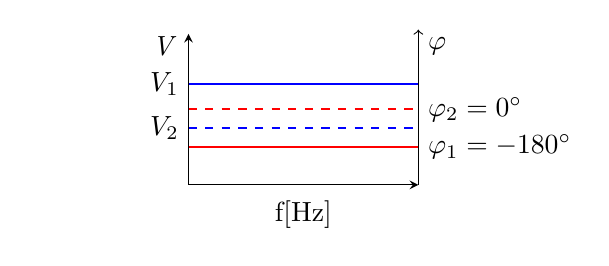
\begin{tikzpicture}[scale=1, transform shape]
    \begin{axis}[
        width=4.5cm, % Breite des Graphen
        height=3.5cm, % Höhe des Graphen
        xmin=0, xmax=10,
        ymin=0, ymax=120,
        axis lines=left,
        axis on top=true,
        domain=0:10,
        xtick=\empty,
        ytick=\empty,
        ylabel style={rotate=270, anchor=east, yshift=0.8cm},
         ylabel={\it V},
        xlabel={f[Hz]},
        clip mode=individual % Verhindert das Abschneiden von Elementen
        ]
        \addplot+[mark=none, thick, blue] coordinates {(0,80) (10,80)};
        \addplot+[mark=none, thick, blue, dashed] coordinates {(0,45) (10,45)};
        % Adding the left-side label
        \node[anchor=east] at (axis cs:0,80) {$V_1$};
        \node[anchor=east] at (axis cs:0,45) {$V_2$};
    \end{axis}
    \begin{axis}[
        width=4.5cm, % Breite des Graphen
        height=3.5cm, % Höhe des Graphen
        xmin=0, xmax=10,
        ymin=-180, ymax=180,
        axis y line*=right,
        axis x line=none,
        ytick=\empty,
        ylabel={$\varphi$},
        ylabel style={rotate=270, anchor=west, yshift=0.8cm},
        clip mode=individual, % Verhindert das Abschneiden von Elementen
        after end axis/.code={
            \draw[->] (axis cs:10,180) -- (axis cs:10,190);
        }
        ]
        \addplot+[mark=none, thick, red, dashed] coordinates {(0,0) (10,0)};
        \addplot+[mark=none, thick, red] coordinates {(0,-90) (10,-90)};
        \node[anchor=west] at (axis cs:10,0) {$\varphi_2 = 0^\circ$};
        \node[anchor=west] at (axis cs:10,-90) {$\varphi_1 = -180^\circ$};
   
   
        \path[draw=none] (axis cs:-7, 0) rectangle (axis cs:16.6,120);
   
   
   
   
    \end{axis}
    \end{tikzpicture}
 \end{center}
 \vspace{1ex}
 \[
 \begin{aligned}
    {U_A} = {U_{{\textnormal{E2}}}} \cdot \underbrace{ \frac{R_1 + R_2}{R_1} \cdot \frac{R_4}{R_3 + R_4}}_{V_2} - U_{\textnormal{E1}} \cdot \underbrace{\frac{R_2}{R_1}}_{V_1}
\end{aligned}
 \]
     &
     Wenn alle Widerstände gleich groß sind, wird die Differenz der Signale $U_{E1}$ und $U_{E2}$ gebildet, weswegen diese Schaltung als Differenzverstärker bezeichnet wird \\
    \hline
    \end{tabular}
    \end{table}
    }
\end{frame}

\begin{frame}
    \b{
    \frametitle{Subtrahierer neu}
    \begin{columns}
        \column{0.48\textwidth}
        \centering
        \begin{figure}
    \centering

    \begin{subfigure}{\linewidth}
        \centering
        \resizebox{0.6\linewidth}{!}{\begin{circuitikz}[scale=0.7, transform shape]
    \ctikzset{
          resistors/scale=0.8,              
          tripoles/en amp/height=1.4, % Höhe des OPV             
          tripoles/en amp/width=1.4,   % Breite des OPV
         tripoles/en amp/input height=0.45
     }
     \draw
     (0,0) node[en amp] (opamp) {}
     (opamp.-) to[R, l_=$R_1$, o-] ++(-1.2,0) to[short, o-] ++(0,0) node[left] {$U_{E1}$}
     (opamp.+) node[circ] {} to[R,  l_=$R_4$] ++(0,-1.5) node[ground] {}
     (opamp.-) node[circ] {} -- ++(0,1) to[R, l=$R_2$] ++(1.9,0) -| (opamp.out)
     (opamp.out) to[short, *-o] ++(0.2,0) node[right] {$U_{A}$}
     (opamp.+) to[R, l_=$R_3$, *-] ++(-1.2,0) to[short, o-] ++(0,0) node[left] {$U_{E2}$};
 \end{circuitikz}}
        \caption{Schaltung eines Subtrahierers}
    \end{subfigure}

    \vspace{0.5cm} 

    \begin{subfigure}{\linewidth}
        \centering
        \resizebox{0.6\linewidth}{!}{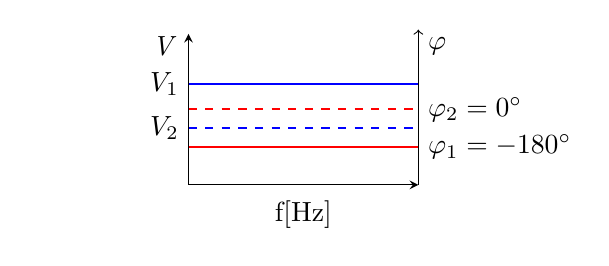
\begin{tikzpicture}[scale=1, transform shape]
    \begin{axis}[
        width=4.5cm, % Breite des Graphen
        height=3.5cm, % Höhe des Graphen
        xmin=0, xmax=10,
        ymin=0, ymax=120,
        axis lines=left,
        axis on top=true,
        domain=0:10,
        xtick=\empty,
        ytick=\empty,
        ylabel style={rotate=270, anchor=east, yshift=0.8cm},
         ylabel={\it V},
        xlabel={f[Hz]},
        clip mode=individual % Verhindert das Abschneiden von Elementen
        ]
        \addplot+[mark=none, thick, blue] coordinates {(0,80) (10,80)};
        \addplot+[mark=none, thick, blue, dashed] coordinates {(0,45) (10,45)};
        % Adding the left-side label
        \node[anchor=east] at (axis cs:0,80) {$V_1$};
        \node[anchor=east] at (axis cs:0,45) {$V_2$};
    \end{axis}
    \begin{axis}[
        width=4.5cm, % Breite des Graphen
        height=3.5cm, % Höhe des Graphen
        xmin=0, xmax=10,
        ymin=-180, ymax=180,
        axis y line*=right,
        axis x line=none,
        ytick=\empty,
        ylabel={$\varphi$},
        ylabel style={rotate=270, anchor=west, yshift=0.8cm},
        clip mode=individual, % Verhindert das Abschneiden von Elementen
        after end axis/.code={
            \draw[->] (axis cs:10,180) -- (axis cs:10,190);
        }
        ]
        \addplot+[mark=none, thick, red, dashed] coordinates {(0,0) (10,0)};
        \addplot+[mark=none, thick, red] coordinates {(0,-90) (10,-90)};
        \node[anchor=west] at (axis cs:10,0) {$\varphi_2 = 0^\circ$};
        \node[anchor=west] at (axis cs:10,-90) {$\varphi_1 = -180^\circ$};
   
   
        \path[draw=none] (axis cs:-7, 0) rectangle (axis cs:16.6,120);
   
   
   
   
    \end{axis}
    \end{tikzpicture}}
        \caption{Frequenzgang eines Subtrahierers}
    \end{subfigure}

\end{figure}

        \column{0.48\textwidth}
        \raggedleft
        \begin{itemize}
            \item Gleichung:
          \[
 {U_A} = {U_{{\textnormal{E2}}}} \cdot \underbrace{ \frac{R_1 + R_2}{R_1} \cdot \frac{R_4}{R_3 + R_4}}_{V_2} - U_{\textnormal{E1}} \cdot \underbrace{\frac{R_2}{R_1}}_{V_1}
          \]
    \item Wenn alle Widerstände gleich groß sind, wird die Differenz der Signale $U_{E1}$ und $U_{E2}$ gebildet, weswegen diese Schaltung als Differenzverstärker bezeichnet wird
        \end{itemize}
    \end{columns}
    }
\end{frame}


%Folie Integrierer

\begin{frame}
    \b{
    \frametitle{Integrierer}
    \centering
    \begin{table}[ht]
    \label{tab:Integrierer}
    \begin{tabular}{|m{0.24\textwidth}|m{0.405\textwidth}|m{0.25\textwidth}|}
    \hline
    Schaltung & Frequenzgang und Gleichung & Erläuterung und Eigenschaften\\ % Neue Zeile mit Text
    \hline
    \vspace{0.5cm}
    \centering
    \begin{circuitikz}[scale=0.7, transform shape]
    \ctikzset{
          resistors/scale=0.8,              
          tripoles/en amp/height=1.4, % Höhe des OPV             
          tripoles/en amp/width=1.4,   % Breite des OPV
         capacitors/scale=0.5,
         tripoles/en amp/input height=0.45
     }
     \vspace{1ex}
     \draw (2,0) node[en amp] (opamp) {}
     (opamp.+) --++ (-0.5,0) node[ground] {} 
     (opamp.out) --++ (0.2,0) node[ocirc, label=right:$U_A$] {}
     (opamp.-) -- ++(0, 0) to[R, l_=$R_1$] ++(-1.2, 0) node[ocirc, label=left:$U_E$] {}
     
     (opamp.out) node[circ] {} -- ++(0,1.5) to[C, l_=$C_1$, *-] ++(-1.9,0) node[circ]{}
     (opamp.out) node[circ] {} -- ++(0,2.8) to[R, l_=$R_2$] ++(-1.9,0) -- ++(0, -2.35) node[circ] {};
     \end{circuitikz}
     & 
     \begin{center}
    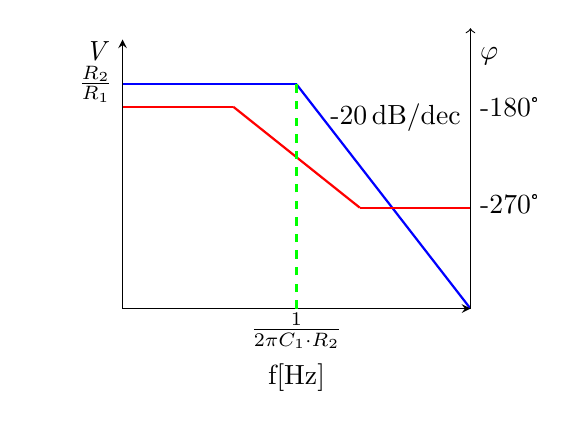
\begin{tikzpicture}[scale=1, transform shape]
    \begin{axis}[
       width=6cm, % Breite des Graphen
       height=5cm, % Höhe des Graphen
        xmin=0, xmax=11,
        ymin=0, ymax=1.2,
        axis lines=center,
        axis on top=true,
        domain=0:10,
        xtick=\empty,
        ytick=\empty,
        ylabel style={xshift=-0.6cm, yshift=0.1cm },
       ylabel={\it V},
       xlabel style={yshift=-0.4cm },
        xlabel={f[Hz]},
        clip mode=individual, % Verhindert das Abschneiden von Elementen
        xlabel style={at={(axis description cs:0.5,-0.05)},anchor=north}
        ]

        \path[draw=none] (axis cs:-3, 0) rectangle (axis cs:13,1);



        \addplot+[mark=none, thick, blue] coordinates {(0,1) (5.5,1)};
        \addplot+[mark=none, thick, blue] coordinates {(5.5,1) (11,0)};
        \node[anchor=east] at (axis cs:0,1) {$\frac{R_2}{R_1}$};
       \node[anchor=east] at (axis cs:11,0.85) {-20\,\text{dB/dec}};
    \end{axis}
    
    \begin{axis}[
       width=6cm, % Breite des Graphen
       height=5cm, % Höhe des Graphen
       xmin=0, xmax=11,
       ymin=0, ymax=240, 
       axis y line*=right,
       axis x line=none,
       ylabel={$\varphi$},
       ylabel style={rotate=270, anchor=west, yshift=1.5cm},
       xtick=\empty,
       ytick=\empty,
       clip mode=individual, % Verhindert das Abschneiden von Elementen
       after end axis/.code={
           \draw[->] (axis cs:11,240) -- (axis cs:11,250);
       }
        ]
        \addplot+[mark=none, thick, red] coordinates {(0,180) (3.5,180)};
        \addplot+[mark=none, thick, red] coordinates {(3.5,180) (7.5,90)};
        \addplot+[mark=none, thick, red] coordinates {(7.5,90) (11,90)};
        \addplot+[mark=none,dashed, thick, green] coordinates {(5.5,0) (5.5,200)};
        \node[] at (axis cs:5.5,-20) {$\frac{1}{2 \pi C_1 \cdot R_2}$};
        \node[anchor=west] at (axis cs:11,180) {-180°};
        \node[anchor=west] at (axis cs:11,93) {-270°};
    \end{axis}
    \end{tikzpicture}
     \[
     U_A(t) = - \frac{R_2}{R_1} U_{\textnormal{E}}(t) - \int_0^t \frac{U_{\textnormal{E}}(t)}{R_1 C_1} \, dt
     \]
     \end{center} 
     &
    \begin{itemize}
        \item Nimmt eine Integration des Eingangssignals vor
        \item Wird als aktives Tiefpassfilter verwendet
    \end{itemize} \\
    \hline
    \end{tabular}
    \end{table}
    }
\end{frame}

\begin{frame}
    \b{
    \frametitle{Integrierer neu}
    \begin{columns}
        \column{0.48\textwidth}
        \centering
        \begin{figure}
    \centering

    \begin{subfigure}{\linewidth}
        \centering
        \resizebox{0.6\linewidth}{!}{\begin{circuitikz}[scale=0.7, transform shape]
    \ctikzset{
          resistors/scale=0.8,              
          tripoles/en amp/height=1.4, % Höhe des OPV             
          tripoles/en amp/width=1.4,   % Breite des OPV
         capacitors/scale=0.5,
         tripoles/en amp/input height=0.45
     }
     \vspace{1ex}
     \draw (2,0) node[en amp] (opamp) {}
     (opamp.+) --++ (-0.5,0) node[ground] {} 
     (opamp.out) --++ (0.2,0) node[ocirc, label=right:$U_A$] {}
     (opamp.-) -- ++(0, 0) to[R, l_=$R_1$] ++(-1.2, 0) node[ocirc, label=left:$U_E$] {}
     
     (opamp.out) node[circ] {} -- ++(0,1.5) to[C, l_=$C_1$, *-] ++(-1.9,0) node[circ]{}
     (opamp.out) node[circ] {} -- ++(0,2.8) to[R, l_=$R_2$] ++(-1.9,0) -- ++(0, -2.35) node[circ] {};
     \end{circuitikz}}
        \caption{Schaltung eines Integrierers}
    \end{subfigure}

    \vspace{0.5cm} 

    \begin{subfigure}{\linewidth}
        \centering
        \resizebox{0.6\linewidth}{!}{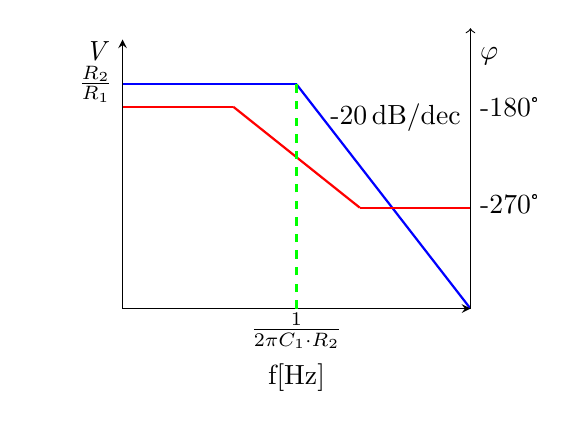
\begin{tikzpicture}[scale=1, transform shape]
    \begin{axis}[
       width=6cm, % Breite des Graphen
       height=5cm, % Höhe des Graphen
        xmin=0, xmax=11,
        ymin=0, ymax=1.2,
        axis lines=center,
        axis on top=true,
        domain=0:10,
        xtick=\empty,
        ytick=\empty,
        ylabel style={xshift=-0.6cm, yshift=0.1cm },
       ylabel={\it V},
       xlabel style={yshift=-0.4cm },
        xlabel={f[Hz]},
        clip mode=individual, % Verhindert das Abschneiden von Elementen
        xlabel style={at={(axis description cs:0.5,-0.05)},anchor=north}
        ]

        \path[draw=none] (axis cs:-3, 0) rectangle (axis cs:13,1);



        \addplot+[mark=none, thick, blue] coordinates {(0,1) (5.5,1)};
        \addplot+[mark=none, thick, blue] coordinates {(5.5,1) (11,0)};
        \node[anchor=east] at (axis cs:0,1) {$\frac{R_2}{R_1}$};
       \node[anchor=east] at (axis cs:11,0.85) {-20\,\text{dB/dec}};
    \end{axis}
    
    \begin{axis}[
       width=6cm, % Breite des Graphen
       height=5cm, % Höhe des Graphen
       xmin=0, xmax=11,
       ymin=0, ymax=240, 
       axis y line*=right,
       axis x line=none,
       ylabel={$\varphi$},
       ylabel style={rotate=270, anchor=west, yshift=1.5cm},
       xtick=\empty,
       ytick=\empty,
       clip mode=individual, % Verhindert das Abschneiden von Elementen
       after end axis/.code={
           \draw[->] (axis cs:11,240) -- (axis cs:11,250);
       }
        ]
        \addplot+[mark=none, thick, red] coordinates {(0,180) (3.5,180)};
        \addplot+[mark=none, thick, red] coordinates {(3.5,180) (7.5,90)};
        \addplot+[mark=none, thick, red] coordinates {(7.5,90) (11,90)};
        \addplot+[mark=none,dashed, thick, green] coordinates {(5.5,0) (5.5,200)};
        \node[] at (axis cs:5.5,-20) {$\frac{1}{2 \pi C_1 \cdot R_2}$};
        \node[anchor=west] at (axis cs:11,180) {-180°};
        \node[anchor=west] at (axis cs:11,93) {-270°};
    \end{axis}
    \end{tikzpicture}}
        \caption{Frequenzgang eines Integrierers}
    \end{subfigure}

\end{figure}

        \column{0.48\textwidth}
        \raggedleft
        \begin{itemize}
            \item Gleichung:
           \[
     U_A(t) = - \frac{R_2}{R_1} U_{\textnormal{E}}(t) - \int_0^t \frac{U_{\textnormal{E}}(t)}{R_1 C_1} \, dt
     \]
        \item Nimmt eine Integration des Eingangssignals vor
        \item Wird als aktives Tiefpassfilter verwendet     
    \end{itemize}
    \end{columns}
    }
\end{frame}

%Folie Differenzierer

\begin{frame}
    \b{
    \frametitle{Differenzierer}
    \centering
    \begin{table}[ht]
    \label{tab:Differenzierer}
    \begin{tabular}{|m{0.24\textwidth}|m{0.405\textwidth}|m{0.25\textwidth}|}
    \hline
    Schaltung & Frequenzgang und Gleichung & Erläuterung und Eigenschaften\\ % Neue Zeile mit Text
    \hline
    \vspace{0.5cm}
    \centering
    \begin{circuitikz}[scale=0.7, transform shape]
    \ctikzset{
          resistors/scale=0.8,              
          tripoles/en amp/height=1.4, % Höhe des OPV             
          tripoles/en amp/width=1.4,   % Breite des OPV
         capacitors/scale=0.5,
         tripoles/en amp/input height=0.45
     }
     \draw (2,0) node[en amp] (opamp) {}
     (opamp.+) --++ (-0.5,0) node[ground] {} 
     (opamp.out) --++ (0.2,0) node[ocirc, label=right:$U_A$] {}
     (opamp.-) -- ++(0, 0) to[C, l_=$C_2$] ++(-0.5, 0) to[R, l_=$R_1$] ++(-1.2,0) node[ocirc, label=left:$U_E$] {}
     (opamp.out) node[circ] {} -- ++(0,1.5) to[C, l_=$C_1$, *-] ++(-1.9,0) node[circ]{}
     (opamp.out) node[circ] {} -- ++(0,2.8) to[R, l_=$R_2$] ++(-1.9,0) -- ++(0, -2.35) node[circ] {};
  
 \end{circuitikz}
    &
    \begin{center}
    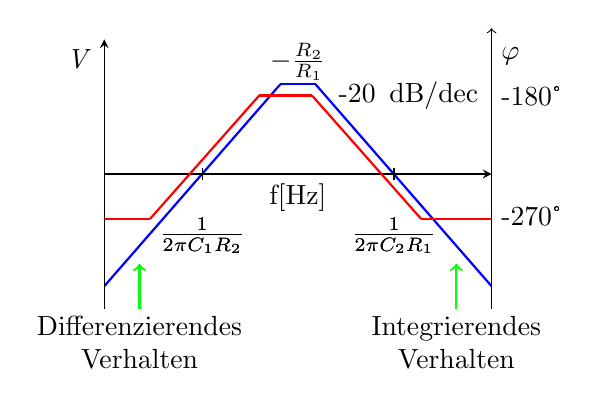
\begin{tikzpicture}[scale=1, transform shape]
    \begin{axis}[
        width=6.5cm, % Breite des Graphen
        height=5cm, % Höhe des Graphen
        xmin=0, xmax=11,
        ymin=-1.2, ymax=1.2,
        axis lines=center,
        axis on top=true,
        domain=0:10,
        clip mode=individual, % Verhindert das Abschneiden von Elementen
        xtick=\empty,
        ytick=\empty,
        ylabel style={xshift=-0.6cm},
        ylabel={\it V},
        xlabel={f[Hz]},
        xlabel style={at={(axis description cs:0.5,0.5)},anchor=north}
        ]
        \path[draw=none] (axis cs:-2, 0) rectangle (axis cs:13,1); \path[draw=none] (axis cs:-2, 0) rectangle (axis cs:13,1);


        \addplot+[mark=none, thick, blue] coordinates {(0,-1) (5,0.8)};
        \addplot+[mark=none, thick, blue] coordinates {(5,0.8) (6,0.8)};
        \addplot+[mark=none, thick, blue] coordinates {(6,0.8) (11,-1)};
        \node[anchor=north] at (axis cs:5.5,1.25) {$-\frac{R_2}{R_1}$};
        \addplot+[only marks, mark=|, black] coordinates {(2.78,0)} node[anchor=south] at (axis cs:2.78,-0.8) {$\frac{1}{2 \pi C_1 R_2}$};
        \addplot+[only marks, mark=|, black] coordinates {(8.23,0)} node[anchor=south] at (axis cs:8.23,-0.8) {$\frac{1}{2\pi C_2 R_1}$};
        \node[anchor=east] at (axis cs:10.9,0.7) {-20\, \text{dB/dec}};
        \addplot+[only marks, mark=|, black] coordinates {(2.78,0)} node[anchor=south] at (axis cs:2.78,-0.8) {$\frac{1}{2 \pi C_1 R_2}$};
        \addplot+[only marks, mark=|, black] coordinates {(8.23,0)} node[anchor=south] at (axis cs:8.23,-0.8) {$\frac{1}{2\pi C_2 R_1}$};
        \draw[->, thick, green] (axis cs:1,-1.2) -- (axis cs:1,-0.8);
        \node[align=center, black] at (axis cs:1,-1.5) {Differenzierendes\\ Verhalten};
        
        \draw[->, thick, green] (axis cs:10,-1.2) -- (axis cs:10,-0.8);
        \node[align=center, black] at (axis cs:10,-1.5) {Integrierendes\\ Verhalten};
        
    \end{axis}
    
    \begin{axis}[
        width=6.5cm, % Breite des Graphen
        height=5cm, % Höhe des Graphen
        xmin=0, xmax=11,
        ymin=0, ymax=240, 
        axis y line*=right,
        axis x line=none,
        ylabel={$\varphi$},
        ylabel style={rotate=270, anchor=west, yshift=1.5cm},
        xtick=\empty,
        ytick=\empty,
        clip mode=individual, % Verhindert das Abschneiden von Elementen
        after end axis/.code={
            \draw[->] (axis cs:11,240) -- (axis cs:11,250);
        }
        ]
        \addplot+[mark=none, thick, red] coordinates {(0,80) (1.3,80)};
        \addplot+[mark=none, thick, red] coordinates {(1.3,80) (4.4,190)};
        \addplot+[mark=none, thick, red] coordinates {(4.4,190) (5.9,190)};
        \addplot+[mark=none, thick, red] coordinates {(5.9,190) (9,80)};
        \addplot+[mark=none, thick, red] coordinates {(9,80) (11,80)};
        \node[anchor=west] at (axis cs:11,82.5) {-270°};
        \node[anchor=west] at (axis cs:11,190) {-180°};
       
    \end{axis}

    
    \end{tikzpicture}
    \begin{multline*}
        U_A = - \frac{R_2}{R_1} U_{\textnormal{E}}(t) \\
        - \int_0^t \frac{1}{R_1 C_1} U_{\textnormal{E}}(t) \, dt 
        - R_2 C_2\frac{dU_{\textnormal{E}}(t)}{dt}
    \end{multline*}
    \end{center} 
    & 
    \textbf{Differenzierer}\newline
    \begin{itemize}
        \item Nimmt eine Integration des Eingangssignals vor
        \item Wird als aktives Hochpassfilter verwendet (zeigt in der Realität meist Bandpassverhalten, wie hier dargestellt)
    \end{itemize} \\
    \hline
    \end{tabular}
    \end{table}
    }
\end{frame}

\begin{frame}
    \b{
    \frametitle{Differenzierer neu}
    \begin{columns}
        \column{0.48\textwidth}
        \centering
        \begin{figure}
    \centering

    \begin{subfigure}{\linewidth}
        \centering
        \resizebox{0.6\linewidth}{!}{\begin{circuitikz}[scale=0.7, transform shape]
    \ctikzset{
          resistors/scale=0.8,              
          tripoles/en amp/height=1.4, % Höhe des OPV             
          tripoles/en amp/width=1.4,   % Breite des OPV
         capacitors/scale=0.5,
         tripoles/en amp/input height=0.45
     }
     \draw (2,0) node[en amp] (opamp) {}
     (opamp.+) --++ (-0.5,0) node[ground] {} 
     (opamp.out) --++ (0.2,0) node[ocirc, label=right:$U_A$] {}
     (opamp.-) -- ++(0, 0) to[C, l_=$C_2$] ++(-0.5, 0) to[R, l_=$R_1$] ++(-1.2,0) node[ocirc, label=left:$U_E$] {}
     (opamp.out) node[circ] {} -- ++(0,1.5) to[C, l_=$C_1$, *-] ++(-1.9,0) node[circ]{}
     (opamp.out) node[circ] {} -- ++(0,2.8) to[R, l_=$R_2$] ++(-1.9,0) -- ++(0, -2.35) node[circ] {};
  
 \end{circuitikz}}
        \caption{Schaltung eines Differenzierers}
    \end{subfigure}

    \vspace{0.5cm} 

    \begin{subfigure}{\linewidth}
        \centering
        \resizebox{0.6\linewidth}{!}{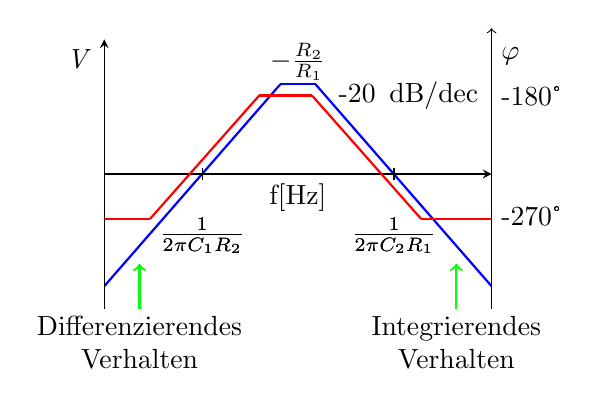
\begin{tikzpicture}[scale=1, transform shape]
    \begin{axis}[
        width=6.5cm, % Breite des Graphen
        height=5cm, % Höhe des Graphen
        xmin=0, xmax=11,
        ymin=-1.2, ymax=1.2,
        axis lines=center,
        axis on top=true,
        domain=0:10,
        clip mode=individual, % Verhindert das Abschneiden von Elementen
        xtick=\empty,
        ytick=\empty,
        ylabel style={xshift=-0.6cm},
        ylabel={\it V},
        xlabel={f[Hz]},
        xlabel style={at={(axis description cs:0.5,0.5)},anchor=north}
        ]
        \path[draw=none] (axis cs:-2, 0) rectangle (axis cs:13,1); \path[draw=none] (axis cs:-2, 0) rectangle (axis cs:13,1);


        \addplot+[mark=none, thick, blue] coordinates {(0,-1) (5,0.8)};
        \addplot+[mark=none, thick, blue] coordinates {(5,0.8) (6,0.8)};
        \addplot+[mark=none, thick, blue] coordinates {(6,0.8) (11,-1)};
        \node[anchor=north] at (axis cs:5.5,1.25) {$-\frac{R_2}{R_1}$};
        \addplot+[only marks, mark=|, black] coordinates {(2.78,0)} node[anchor=south] at (axis cs:2.78,-0.8) {$\frac{1}{2 \pi C_1 R_2}$};
        \addplot+[only marks, mark=|, black] coordinates {(8.23,0)} node[anchor=south] at (axis cs:8.23,-0.8) {$\frac{1}{2\pi C_2 R_1}$};
        \node[anchor=east] at (axis cs:10.9,0.7) {-20\, \text{dB/dec}};
        \addplot+[only marks, mark=|, black] coordinates {(2.78,0)} node[anchor=south] at (axis cs:2.78,-0.8) {$\frac{1}{2 \pi C_1 R_2}$};
        \addplot+[only marks, mark=|, black] coordinates {(8.23,0)} node[anchor=south] at (axis cs:8.23,-0.8) {$\frac{1}{2\pi C_2 R_1}$};
        \draw[->, thick, green] (axis cs:1,-1.2) -- (axis cs:1,-0.8);
        \node[align=center, black] at (axis cs:1,-1.5) {Differenzierendes\\ Verhalten};
        
        \draw[->, thick, green] (axis cs:10,-1.2) -- (axis cs:10,-0.8);
        \node[align=center, black] at (axis cs:10,-1.5) {Integrierendes\\ Verhalten};
        
    \end{axis}
    
    \begin{axis}[
        width=6.5cm, % Breite des Graphen
        height=5cm, % Höhe des Graphen
        xmin=0, xmax=11,
        ymin=0, ymax=240, 
        axis y line*=right,
        axis x line=none,
        ylabel={$\varphi$},
        ylabel style={rotate=270, anchor=west, yshift=1.5cm},
        xtick=\empty,
        ytick=\empty,
        clip mode=individual, % Verhindert das Abschneiden von Elementen
        after end axis/.code={
            \draw[->] (axis cs:11,240) -- (axis cs:11,250);
        }
        ]
        \addplot+[mark=none, thick, red] coordinates {(0,80) (1.3,80)};
        \addplot+[mark=none, thick, red] coordinates {(1.3,80) (4.4,190)};
        \addplot+[mark=none, thick, red] coordinates {(4.4,190) (5.9,190)};
        \addplot+[mark=none, thick, red] coordinates {(5.9,190) (9,80)};
        \addplot+[mark=none, thick, red] coordinates {(9,80) (11,80)};
        \node[anchor=west] at (axis cs:11,82.5) {-270°};
        \node[anchor=west] at (axis cs:11,190) {-180°};
       
    \end{axis}

    
    \end{tikzpicture}}
        \caption{Frequenzgang eines Differenzierers}
    \end{subfigure}

\end{figure}

        \column{0.48\textwidth}
        \raggedleft
        \begin{itemize}
            \item Gleichung:
           \[
     U_A = - \frac{R_2}{R_1} U_{\textnormal{E}}(t) \\
        - \int_0^t \frac{1}{R_1 C_1} U_{\textnormal{E}}(t) \, dt 
        - R_2 C_2\frac{dU_{\textnormal{E}}(t)}{dt}
     \]
        \item Nimmt eine Integration des Eingangssignals vor
        \item Wird als aktives Hochpassfilter verwendet (zeigt in der Realität meist Bandpassverhalten, wie hier dargestellt)  
    \end{itemize}
    \end{columns}
    }
\end{frame}

%Folie Logarithmierer

\begin{frame}
    \b{
    \frametitle{Logarithmierer}
    \centering
    \begin{table}[ht]
    \label{tab:Logarithmierer}
    \begin{tabular}{|m{0.24\textwidth}|m{0.405\textwidth}|m{0.25\textwidth}|}
    \hline
    Schaltung & Frequenzgang und Gleichung & Erläuterung und Eigenschaften\\ % Neue Zeile mit Text
    \hline
    \vspace{0.5cm}
    \centering
    \begin{circuitikz}[scale=0.7, transform shape]
    \ctikzset{
          resistors/scale=0.8,              
          tripoles/en amp/height=1.4, % Höhe des OPV             
          tripoles/en amp/width=1.4,   % Breite des OPV
         diodes/scale=0.8,
         tripoles/en amp/input height=0.45
     }
     \draw
     (0,0) node[en amp] (opamp) {}
     (opamp.-) to[R, l_=$R_1$, *-] ++(-1.2,0) to[short, o-] ++(0,0) node[left] {$U_E$}
     (opamp.+) -- ++(0,0) node[ground] {}
     (opamp.-) |- ++(0,1.5) to[D, l^=$D_1$] ++(2,0) -| (opamp.out)
     (opamp.out) to[short, *-o] ++(0.2,0) node[right] {$U_{A}$};
 \end{circuitikz}
    &
    \begin{center}
    \[
    U_{\textnormal{A}} =-U_{\textnormal{T}}\cdot \ln{\left(\frac{U_{\textnormal{E}}}{R_1\cdot I_S}\right)}
    \]
        \[
            U_{\textnormal{T}} = \frac{k_{\textnormal{B}} \cdot T}{e}
            \]
            
            \(e = \text{Elementarladung}\)
            
            \(k_{\textnormal{B}} = \text{Boltzmannkonstante}\)
            
            \(I_{\textnormal{s}} = \text{Sperrstrom der Diode}\)
    \end{center} 
    & 
    Bildet den natürlichen Logarithmus des Eingangssignals \\
    \hline
    \end{tabular}
    \end{table}
    }
\end{frame}

\begin{frame}
    \b{
    \frametitle{Logarithmierer neu}
    \begin{columns}
        \column{0.48\textwidth}
        \centering
        \begin{figure}
    \centering
        \begin{circuitikz}[scale=0.7, transform shape]
    \ctikzset{
          resistors/scale=0.8,              
          tripoles/en amp/height=1.4, % Höhe des OPV             
          tripoles/en amp/width=1.4,   % Breite des OPV
         diodes/scale=0.8,
         tripoles/en amp/input height=0.45
     }
     \draw
     (0,0) node[en amp] (opamp) {}
     (opamp.-) to[R, l_=$R_1$, *-] ++(-1.2,0) to[short, o-] ++(0,0) node[left] {$U_E$}
     (opamp.+) -- ++(0,0) node[ground] {}
     (opamp.-) |- ++(0,1.5) to[D, l^=$D_1$] ++(2,0) -| (opamp.out)
     (opamp.out) to[short, *-o] ++(0.2,0) node[right] {$U_{A}$};
 \end{circuitikz}
        \caption{Schaltung eines Logarithmierers}

\end{figure}

        \column{0.48\textwidth}
        \raggedleft
        \begin{itemize}
            \item Gleichung:
           \[
    U_{\textnormal{A}} =-U_{\textnormal{T}}\cdot \ln{\left(\frac{U_{\textnormal{E}}}{R_1\cdot I_S}\right)}
    \]
        \[
            U_{\textnormal{T}} = \frac{k_{\textnormal{B}} \cdot T}{e}
            \]
            
            \(e = \text{Elementarladung}\)
            
            \(k_{\textnormal{B}} = \text{Boltzmannkonstante}\)
            
            \(I_{\textnormal{s}} = \text{Sperrstrom der Diode}\)
        \item Bildet den natürlichen Logarithmus des Eingangssignals
    \end{itemize}
    \end{columns}
    }
\end{frame}

%Folie Potenzierer

\begin{frame}
    \b{
        \frametitle{Potenzierer}
    \centering
    \begin{table}[ht]
    \label{tab:Potenzierer}
    \begin{tabular}{|m{0.24\textwidth}|m{0.405\textwidth}|m{0.25\textwidth}|}
    \hline
    Schaltung & Frequenzgang und Gleichung & Erläuterung und Eigenschaften\\ % Neue Zeile mit Text
    \hline
    \vspace{0.5cm}
    \centering
    \begin{circuitikz}[scale=0.7, transform shape]
    \ctikzset{
          resistors/scale=0.8,              
          tripoles/en amp/height=1.4, % Höhe des OPV            
          tripoles/en amp/width=1.4,   % Breite des OPV
         diodes/scale=0.8,
         tripoles/en amp/input height=0.45
     }
     \draw
     (0,0) node[en amp] (opamp) {}
     (opamp.-) to[D, l_=$D_1$, invert, *-] ++(-1.2,0) to[short, o-] ++(0,0) node[left] {$U_E$}
     (opamp.+) -- ++(0,0) node[ground] {}
     (opamp.-) |- ++(0,1.5) to[R, l^=$R_1$] ++(2,0) -| (opamp.out)
     (opamp.out) to[short, *-o] ++(0.2,0) node[right] {$U_{A}$};
 \end{circuitikz}
    &
    \begin{center}
    \[
    U_{\textnormal{A}} =-R_1\cdot I_{\textnormal{S}} \cdot e^{\frac{U_{\textnormal{E}}}{U_{\textnormal{T}}}}
    \]
    \end{center} 
    & 
    Besitzt einen e-funktionalen Zusammenhang zwischen Ein- und Ausgangsspannung \\
    \hline
    \end{tabular}
    \end{table}
    }
\end{frame}

\begin{frame}
    \b{
    \frametitle{Potenzierer neu}
    \begin{columns}
        \column{0.48\textwidth}
        \centering
        \begin{figure}
        \centering
        \resizebox{0.6\linewidth}{!}{\begin{circuitikz}[scale=0.7, transform shape]
    \ctikzset{
          resistors/scale=0.8,              
          tripoles/en amp/height=1.4, % Höhe des OPV            
          tripoles/en amp/width=1.4,   % Breite des OPV
         diodes/scale=0.8,
         tripoles/en amp/input height=0.45
     }
     \draw
     (0,0) node[en amp] (opamp) {}
     (opamp.-) to[D, l_=$D_1$, invert, *-] ++(-1.2,0) to[short, o-] ++(0,0) node[left] {$U_E$}
     (opamp.+) -- ++(0,0) node[ground] {}
     (opamp.-) |- ++(0,1.5) to[R, l^=$R_1$] ++(2,0) -| (opamp.out)
     (opamp.out) to[short, *-o] ++(0.2,0) node[right] {$U_{A}$};
 \end{circuitikz}}
        \caption{Schaltung eines Potenzierers}

\end{figure}

        \column{0.48\textwidth}
        \raggedleft
        \begin{itemize}
            \item Gleichung:
           \[
    U_{\textnormal{A}} =-R_1\cdot I_{\textnormal{S}} \cdot e^{\frac{U_{\textnormal{E}}}{U_{\textnormal{T}}}}
    \]
        \item Besitzt einen e-funktionalen Zusammenhang zwischen Ein- und Ausgangsspannung
    \end{itemize}
    \end{columns}
    }
\end{frame}

%Folie Insutrmentenverstärker 

\begin{frame}
    \b{
        \frametitle{Instrumentenverstärker}
    \centering
    \begin{table}[ht]
    \label{tab:Instrumentenverstaerker}
    \begin{tabular}{|m{0.24\textwidth}|m{0.405\textwidth}|m{0.25\textwidth}|}
    \hline
    Schaltung & Frequenzgang und Gleichung & Erläuterung und Eigenschaften\\ % Neue Zeile mit Text
    \hline
    \vspace{0.5cm}
    \centering
    \begin{circuitikz}[scale=0.6, transform shape]
    \ctikzset{
         resistors/scale=0.8,              
         tripoles/en amp/height=1.4, % Höhe des OPV             
         tripoles/en amp/width=1.4   % Breite des OPV
    }
    \draw 
    % Erster OPV mit input height=-0.45
    (2,-4.5) node[en amp, noinv input down] (opamp1) {}
    (opamp1.+) --++ (-0.5,0) node[ocirc, label=left:$U_{E2}$] (eingang1) {};
    
   \draw (2,0) node[en amp, noinv input up] (opamp2) {}
    (opamp2.+) --++ (-0.5,0) node[ocirc, label=left:$U_{E1}$] (eingang2) {}
    (opamp1.-)  to[R=$R_g$] (opamp2.-);

   % Dritter OPV mit angepasstem Eingangsabstand
    \ctikzset{tripoles/en amp/input height=0.55} % Anpassung nur für diesen OPV
    \draw (6,-2.25) node[en amp] (opamp3) {}
    (opamp3.-) -- ++(-0.5,0) to[R=$R_1$] ++(-1.5,0) to[R=$R_2$] ++(-2,0) node[circ]{}
    (opamp3.+) -- ++(-0.5,0) to[R=$R_3$] ++(-1.5,0) to[R=$R_4$] ++(-2,0) node[circ]{}
    (opamp2.out) -- ++(0,-1.72) node[circ]{}
    (opamp1.out) -- ++(0,1.72) node[circ]{}
    (opamp3.out) node[circ, label=below:{$U_A$}]{} -- ++(0, 2) to[R=$R_5$] ++(-2,0) -- ++(0, -1.45)node[circ]{};

\end{circuitikz}
     &
         \begin{center}
   \begin{tikzpicture}[scale=1, transform shape]
    \begin{axis}[
        width=4.5cm, % Breite des Graphen
        height=3.5cm, % Höhe des Graphen
        xmin=0, xmax=10,
        ymin=0, ymax=120,
        axis lines=left,
        axis on top=true,
        domain=0:10,
        xtick=\empty,
        ytick=\empty,
        ylabel style={rotate=270, anchor=east, yshift=0.8cm}, % Position der Beschriftung oben links, horizontal
         ylabel={\it V}, % Hier die gewünschte Beschriftung einfügen
        xlabel={f[Hz]},
        clip mode=individual % Verhindert das Abschneiden von Elementen
        ]
        \addplot+[mark=none, thick, blue] coordinates {(0,80) (10,80)};
        % Adding the left-side label
        \node[anchor=east] at (axis cs:0,80) {$\mathit{A}_{\textnormal{A}}$};
    \end{axis}
    \begin{axis}[
        width=4.5cm, % Breite des Graphen
        height=3.5cm, % Höhe des Graphen
        xmin=0, xmax=10,
        ymin=-180, ymax=180,
        axis y line*=right,
        axis x line=none,
        ytick=\empty,
        ylabel={$\varphi$},
        ylabel style={rotate=270, anchor=west, yshift=0.8cm},
        clip mode=individual, % Verhindert das Abschneiden von Elementen
        after end axis/.code={
            \draw[->] (axis cs:10,180) -- (axis cs:10,190);
        }
        ]
        \addplot+[mark=none, thick, red] coordinates {(0,0) (10,0)};
        \node[anchor=west] at (axis cs:10,0) {$\varphi_{\textnormal{A}}$};
    \end{axis}
    \end{tikzpicture}
\end{center}

\vspace{1ex}
\[
\mathit{a_i} : \text{Amplitude Eingangsspannung i}
\]
\[
\mathit{\varphi_i} : \text{Phase Eingangsspannung i}
\]
\[
\mathit{A}_{A} = \sqrt{a_1^2 + a_2^2 + 2a_1a_2 \cos(\varphi_1 - \varphi_2)}
\]
\[
\mathit{\tan}(\varphi_A) = \frac{a_1 \mathit{\sin}(\varphi_1) + a_2 \mathit{\sin}(\varphi_2)}{a_1 \mathit{\cos}(\varphi_1) + a_2 \mathit{\cos}(\varphi_2)}
\]
\[
    \text{Wenn} : R_2 = R_4 = R
\]
\[
    U_{\textnormal{A}} = (1+ \frac{2R} {R_{\textnormal{g}}}) \cdot \frac{R_3} {R_2} (U_{\textnormal{E2}}-U_{\textnormal{E1}})
\]
     & 
    Differenzverstärker mit hoher Eingangsimpedanz und hoher Gleichtaktunterdrückung  
 \\
    \hline
    \end{tabular}
    \end{table}
    }
\end{frame}

\begin{frame}
    \b{
    \frametitle{Instrumentenverstärker neu}
    \begin{columns}
        \column{0.48\textwidth}
        \centering
        \begin{figure}
    \centering

    \begin{subfigure}{\linewidth}
        \centering
        \resizebox{0.6\linewidth}{!}{\begin{circuitikz}[scale=0.6, transform shape]
    \ctikzset{
         resistors/scale=0.8,              
         tripoles/en amp/height=1.4, % Höhe des OPV             
         tripoles/en amp/width=1.4   % Breite des OPV
    }
    \draw 
    % Erster OPV mit input height=-0.45
    (2,-4.5) node[en amp, noinv input down] (opamp1) {}
    (opamp1.+) --++ (-0.5,0) node[ocirc, label=left:$U_{E2}$] (eingang1) {};
    
   \draw (2,0) node[en amp, noinv input up] (opamp2) {}
    (opamp2.+) --++ (-0.5,0) node[ocirc, label=left:$U_{E1}$] (eingang2) {}
    (opamp1.-)  to[R=$R_g$] (opamp2.-);

   % Dritter OPV mit angepasstem Eingangsabstand
    \ctikzset{tripoles/en amp/input height=0.55} % Anpassung nur für diesen OPV
    \draw (6,-2.25) node[en amp] (opamp3) {}
    (opamp3.-) -- ++(-0.5,0) to[R=$R_1$] ++(-1.5,0) to[R=$R_2$] ++(-2,0) node[circ]{}
    (opamp3.+) -- ++(-0.5,0) to[R=$R_3$] ++(-1.5,0) to[R=$R_4$] ++(-2,0) node[circ]{}
    (opamp2.out) -- ++(0,-1.72) node[circ]{}
    (opamp1.out) -- ++(0,1.72) node[circ]{}
    (opamp3.out) node[circ, label=below:{$U_A$}]{} -- ++(0, 2) to[R=$R_5$] ++(-2,0) -- ++(0, -1.45)node[circ]{};

\end{circuitikz}}
        \caption{Schaltung eines Instrumentenverstärkers}
    \end{subfigure}

    \vspace{0.5cm} 

    \begin{subfigure}{\linewidth}
        \centering
        \resizebox{0.6\linewidth}{!}{\begin{tikzpicture}[scale=1, transform shape]
    \begin{axis}[
        width=4.5cm, % Breite des Graphen
        height=3.5cm, % Höhe des Graphen
        xmin=0, xmax=10,
        ymin=0, ymax=120,
        axis lines=left,
        axis on top=true,
        domain=0:10,
        xtick=\empty,
        ytick=\empty,
        ylabel style={rotate=270, anchor=east, yshift=0.8cm}, % Position der Beschriftung oben links, horizontal
         ylabel={\it V}, % Hier die gewünschte Beschriftung einfügen
        xlabel={f[Hz]},
        clip mode=individual % Verhindert das Abschneiden von Elementen
        ]
        \addplot+[mark=none, thick, blue] coordinates {(0,80) (10,80)};
        % Adding the left-side label
        \node[anchor=east] at (axis cs:0,80) {$\mathit{A}_{\textnormal{A}}$};
    \end{axis}
    \begin{axis}[
        width=4.5cm, % Breite des Graphen
        height=3.5cm, % Höhe des Graphen
        xmin=0, xmax=10,
        ymin=-180, ymax=180,
        axis y line*=right,
        axis x line=none,
        ytick=\empty,
        ylabel={$\varphi$},
        ylabel style={rotate=270, anchor=west, yshift=0.8cm},
        clip mode=individual, % Verhindert das Abschneiden von Elementen
        after end axis/.code={
            \draw[->] (axis cs:10,180) -- (axis cs:10,190);
        }
        ]
        \addplot+[mark=none, thick, red] coordinates {(0,0) (10,0)};
        \node[anchor=west] at (axis cs:10,0) {$\varphi_{\textnormal{A}}$};
    \end{axis}
    \end{tikzpicture}}
        \caption{Frequenzgang eines Instrumentenverstärkers}
    \end{subfigure}

\end{figure}

        \column{0.48\textwidth}
        \raggedleft
        \begin{itemize}
            \item Gleichung:
         \[
\mathit{a_i} : \text{Amplitude Eingangsspannung i}
\]
\[
\mathit{\varphi_i} : \text{Phase Eingangsspannung i}
\]
\[
\mathit{A}_{A} = \sqrt{a_1^2 + a_2^2 + 2a_1a_2 \cos(\varphi_1 - \varphi_2)}
\]
\[
\mathit{\tan}(\varphi_A) = \frac{a_1 \mathit{\sin}(\varphi_1) + a_2 \mathit{\sin}(\varphi_2)}{a_1 \mathit{\cos}(\varphi_1) + a_2 \mathit{\cos}(\varphi_2)}
\]
\[
    \text{Wenn} : R_2 = R_4 = R
\]
\[
    U_{\textnormal{A}} = (1+ \frac{2R} {R_{\textnormal{g}}}) \cdot \frac{R_3} {R_2} (U_{\textnormal{E2}}-U_{\textnormal{E1}})
\]
        \item Differenzverstärker mit hoher Eingangsimpedanz und hoher Gleichtaktunterdrückung    
    \end{itemize}
    \end{columns}
    }
\end{frame}


%Folie Insutrmentenverstärker 

\begin{frame}
    \b{
        \frametitle{Impedanzwandler}
    \centering
    \begin{table}[ht]
    \label{tab:Impedanzwandler}
    \begin{tabular}{|m{0.24\textwidth}|m{0.405\textwidth}|m{0.25\textwidth}|}
    \hline
    Schaltung & Frequenzgang und Gleichung & Erläuterung und Eigenschaften\\ % Neue Zeile mit Text
    \hline
    \vspace{0.5cm}
    \centering
    \scalebox{0.45}{\begin{circuitikz}
    \ctikzset{tripoles/en amp/input height=0.45}
\draw (0,0)node[en amp, en amp text A](E){}
    (E.out)
    (E.-)
    (E.+);
\draw (E.-) -- (-1.5,0.5) -- (-1.5,2) -- (2,2) to[short,-*] (2,0);
\draw (E.out) to[short, -o] ( 3,0);
\draw (3,-2) to[short, o-o] (-3,-2);
\draw (0,-2)node[ground]{};
\draw (E.+) to[short,-o] (-3,-0.5);


\draw (-3,-0.5) to[open,v>, name=ue] (-3,-2);
\draw (3,0) to[open,v>, name=ua] (3,-2);
\varrmore{ua}{$U_\mathrm{A}$};
\varrmore{ue}{$U_\mathrm{E}$};
\end{circuitikz}}
     &

\vspace{1ex}
Ausgangsspannung $U_\mathrm{A}$ folgt der Eingangsspannung $U_\mathrm{E}$ \newline
Verstärkung $V = \frac{U_\mathrm{A}}{U_\mathrm{E}} = 1$ 

     & 
    
     Auch Spannungsfolger genannt \newline
     Hoher Eingangswiderstand durch Operationsverstärker \newline
     Typische Anwendung: Sensoren

 \\
    \hline
    \end{tabular}
    \end{table}
    }
\end{frame}

\begin{frame}
    \b{
    \frametitle{Impedanzwandler neu}
    \begin{columns}
        \column{0.48\textwidth}
        \centering
        \begin{figure}
        \centering
        \resizebox{0.6\linewidth}{!}{\begin{circuitikz}
    \ctikzset{tripoles/en amp/input height=0.45}
\draw (0,0)node[en amp, en amp text A](E){}
    (E.out)
    (E.-)
    (E.+);
\draw (E.-) -- (-1.5,0.5) -- (-1.5,2) -- (2,2) to[short,-*] (2,0);
\draw (E.out) to[short, -o] ( 3,0);
\draw (3,-2) to[short, o-o] (-3,-2);
\draw (0,-2)node[ground]{};
\draw (E.+) to[short,-o] (-3,-0.5);


\draw (-3,-0.5) to[open,v>, name=ue] (-3,-2);
\draw (3,0) to[open,v>, name=ua] (3,-2);
\varrmore{ua}{$U_\mathrm{A}$};
\varrmore{ue}{$U_\mathrm{E}$};
\end{circuitikz}}
        \caption{Schaltung eines Impedanzwandlers}

\end{figure}

        \column{0.48\textwidth}
        \raggedleft
        \begin{itemize}
            \item Gleichung:
           \[
    U_{\textnormal{A}} =-R_1\cdot I_{\textnormal{S}} \cdot e^{\frac{U_{\textnormal{E}}}{U_{\textnormal{T}}}}
    \]
        \item Ausgangsspannung $U_\mathrm{A}$ folgt der Eingangsspannung $U_\mathrm{E}$ 
        \item Verstärkung $V = \frac{U_\mathrm{A}}{U_\mathrm{E}} = 1$ 
        \item Auch Spannungsfolger genannt
        \item Hoher Eingangswiderstand durch Operationsverstärker
        \item Typische Anwendung: Sensoren
    \end{itemize}
    \end{columns}
    }
\end{frame}				%Rückkopplung, Frequenzverhalten und Stabilität
\begin{frame}
    \fta{Stabilität von Verstärkerschaltungen}
    \s{
    Durch die Rückführung des Ausgangssignals auf das Eingangssignal ergibt sich ein Regelkreis. Dieser Regelkreis ist allerdings nicht immer stabil, d.h. die Rückführung führt nicht dazu, dass die Ausgangsgröße sich nur so lange ändert, wie am Eingang auch eine Differenzspannung vorliegt\footnote{Dies ist eine Vereinfachung. In der Regelungstechnik wird zwischen Lyapunov-Stabilität und BIBO-Stabilität unterschieden (siehe hierzu z.B. \glqq Regelungstechnik\grqq{} von Otto Föllinger)}.
    Dies wird deutlich, wenn das Ausgangssignal auf den nicht-invertierenden anstatt den invertierenden Eingang zurückgeführt wird. Wird nun eine Spannungssdifferenz an den Eingang angelegt und am Ausgang verstärkt ausgegeben, so führt diese Ausgangsspannung zu einer erneuten Erhöhung der Spannungsdifferenz am Eingang. 
    Das System ist also nicht stabil. Ein ähnliches Phänomen kann beobachtet werden, wenn in der Verstärkerschaltung Energiespeicher (Kondensatoren oder Spulen) verwendet werden. Eine solche Schaltung weißt immer eine Stabilitätsgrenze auf, die dann erreicht wird, wenn das auf den invertierenden Eingang rückgekoppelte Signal, eine Phasenverschiebung von 180$^{\circ}$ aufweist.
    In diesem Fall wird die Gegenkopplung zur Mitkopplung und die Schaltung wird instabil. 
    Das ist aber nicht die einzige Möglichkeit, wie eine Schaltung instabil werden kann. Auch kann die Schaltung ins Schwingen geraten, wenn die Energiespeicher nicht richtig dimensioniert werden. Aus diesem Grund sind Stabilitätsanalysen der entworfenen Schaltungen unerlässlich. 
    
    Es sollen im Rahmen dieses Kapitels folgende Kompetenzen erworben werden:


%\speech{1}{
%    Stabilität von Verstärkerschaltungen
%    Durch die Rückführung des Ausgangssignals auf das Eingangssignal ergibt sich ein Regelkreis. Dieser Regelkreis ist allerdings nicht immer stabil, d.h. die Rückführung führt nicht dazu, dass die Ausgangsgröße sich nur so lange ändert, wie am Eingang auch eine Differenzspannung vorliegt\footnote{Dies ist eine Vereinfachung. In der Regelungstechnik wird zwischen Lyapunov-Stabilität und BIBO-Stabilität unterschieden (siehe hierzu z.B. \glqq Regelungstechnik\grqq{} von Otto Föllinger)}.
%    Dies wird deutlich, wenn das Ausgangssignal auf den nicht-invertierenden anstatt den invertierenden Eingang zurückgeführt wird. Wird nun eine Spannungssdifferenz an den Eingang angelegt und am Ausgang verstärkt ausgegeben, so führt diese Ausgangsspannung zu einer erneuten Erhöhung der Spannungsdifferenz am Eingang.
%    Das System ist also nicht stabil. Ein ähnliches Phänomen kann beobachtet werden, wenn in der Verstärkerschaltung Energiespeicher (Kondensatoren oder Spulen) verwendet werden. Eine solche Schaltung weißt immer eine Stabilitätsgrenze auf, die dann erreicht wird, wenn das auf den invertierenden Eingang rückgekoppelte Signal, eine Phasenverschiebung von 180$^{\circ}$ aufweist.
%    In diesem Fall wird die Gegenkopplung zur Mitkopplung und die Schaltung wird instabil.
%    Das ist aber nicht die einzige Möglichkeit, wie eine Schaltung instabil werden kann. Auch kann die Schaltung ins Schwingen geraten, wenn die Energiespeicher nicht richtig dimensioniert werden. Aus diesem Grund sind Stabilitätsanalysen der entworfenen Schaltungen unerlässlich.
%    Es sollen im Rahmen dieses Kapitels folgende Kompetenzen erworben werden:
%}
    \s{
        \begin{Lernziele}{Operationsverstärker}
            \title{Lernziele: Stabilität von Verstärkerschaltungen}
            Die Studierenden können
            \begin{itemize}
                \item Stabilitätsanalysen durchführen und Ergebnisse der Analyse beurteilen.
                \item Bauteile in OPV-Schaltungen dem Stabilitätskriterien entsprechend dimensionieren.
            \end{itemize}
        \end{Lernziele}
    }
    

%\speech{1}{
%    Lernziele
%    Die Studierenden können Stabilitätsanalysen durchführen und Ergebnisse der Analyse beurteilen. Sie können Bauteile in OPV-Schaltungen dem Stabilitätskriterien entsprechend dimensionieren.
%}
    Einige der Stabilitätskriterien, die zur Stabilitätsbewertung herangezogen werden sind im Folgenden beschrieben.
    Die Bewertung der Stabilität von Operationsverstärkerschaltungen ist eine wichtige Fähigkeit für Studierende der Elektrotechnik, egal ob die Schaltungen von Grund auf entworfen oder Fehler in bestehenden Schaltungen behoben werden sollen. 
    Diese Bewertung stellt sicher, dass Operationsverstärkerschaltungen zuverlässig und effektiv arbeiten, was für ihre Integration in verschiedene elektronische Systeme unerlässlich ist. Im Folgenden wird erläutert, welche Methoden zur Bewertung der Stabilität verwendet werden.

   %\speech{1}{
   % Einige der Stabilitätskriterien, die zur Stabilitätsbewertung herangezogen werden sind im Folgenden beschrieben.
   % Die Bewertung der Stabilität von Operationsverstärkerschaltungen ist eine wichtige Fähigkeit für Studierende der Elektrotechnik, egal ob die Schaltungen von Grund auf entworfen oder Fehler in bestehenden Schaltungen behoben werden sollen. 
   % Diese Bewertung stellt sicher, dass Operationsverstärkerschaltungen zuverlässig und effektiv arbeiten, was für ihre Integration in verschiedene elektronische Systeme unerlässlich ist. 
   % Im Folgenden wird erläutert, welche Methoden zur Bewertung der Stabilität verwendet werden.
   % }
   } 
	\b{\frametitle{Stabilität des Operationsverstärker-Regelkreis}
    Durch die Rückführung des Ausgangssignal ergibt sich ein Regelkreis. Dieser muss auf Stabilität überprüft werden. Dazu werden 3 Methoden vorgstellt:
    \begin{itemize}
    \item Die Frequengangzanalyse auf Grundlage des Bodediagramms
    \item Die Untersuchung der Übertragungsfunktion auf ihre Pollagen
    \item Die Analyse des Einschwingverhaltens
    \end{itemize}}
\end{frame}

%Frequenzganganalyse
\begin{frame}
    \frametitle{Frequenzgangsanalyse (experimentell/simulativ)}
    \s{
    Eine grundlegende Technik ist die Frequenzganganalyse. 
    Bei diesem Verfahren wird untersucht, wie sich die Verstärkung und die Phase einer Operationsverstärkerschaltung ändern, wenn die Frequenz des Eingangssignals variiert. Werkzeuge wie Bodediagramme werden häufig zur Visualisierung dieser Reaktion eingesetzt und helfen bei der Identifizierung potenzieller Stabilitätsprobleme wie Verstärkungsspitzen oder Phasenverschiebungen, die zu Instabilität führen könnten.
    Ein wichtiges Kriterium bildet hier die Phasenreserve. Die Bestimmung dieser Größe ist ein quantitativer Ansatz zur Stabilitätsbewertung. Sie hilft bei der Messung der Stabilitätsspanne innerhalb eines Rückkopplungssystems, indem sie die Phasendifferenz zwischen der tatsächlichen Phasenverschiebung bei der Durchtrittsfrequenz (also 0 dB) und 180$^{\circ}$ betrachtet. Dieser Punkt wird als \glqq kritischer Punkt\grqq{} bezeichnet, da bei einer Phasenverschiebung über 180$^{\circ}$ und einer Verstärkung über 0 dB, die Rückkopplung zur Mitkopplung wird. 
    Wenn die Phasendifferenz einen bestimmten Schwellenwert überschreitet, in der Regel etwa 45$^{\circ}$, wird davon ausgegangen, dass das System weit genug von der Stabilitätsgrenze entferent ist.
    Diese Analyse findet normalerweise graphisch auf Grundlage des Bodediagramms statt. 
    }
        \begin{center}
        \b{Bei dieser Methode wird das Bodediagramm im relevanten Frequenzbereich betrachtet.} 
        \f{width=\textwidth}{width=0.9\textwidth}{Bilder/kap4/Amplitudengang Regelkreis und Phasengang.pdf}{Bestimmung der Phasenreserve auf Grundlage des Bodediagramms} 
        \label{fig:Frequenzganganalyse}
    \end{center}
    \b{Auf dieser Grundlage wird die Phasenlage am 0 dB-Durchtrittspunkt der Amplitude bestimmt. Besteht ein geringer Abstand zu -180° ist das System instabil.}  %Inspiration: https://www.google.com/search?client=firefox-b-d&sca_esv=07fc2a91d39bc3b9&sca_upv=1&sxsrf=ADLYWIJlgSTFsuVgmDjND0631smrCLZH5g:1720507056816&q=phasenreserve&udm=2&fbs=AEQNm0A6bwEop21ehxKWq5cj-cHa02QUie7apaStVTrDAEoT1A_pRBhSGXWPGL0_xk71SHFUmHSJWGPXoD9Kj5_rnHbWMOqF2geje-KRnle5TYvzlu3NqubtU_abXJaIrzdDTfJXR1IEap8k1YruTZC6a9-SgzP6gSnzb0vwoljHMAsMGnOtcGrx634vR4spXb0931ZlkiFj&sa=X&ved=2ahUKEwjcztGfrJmHAxUygP0HHerJD6MQtKgLegQIDRAB&biw=1536&bih=835&dpr=1.25#vhid=kWaDK2aKHZdoUM&vssid=mosaic         
    
\end{frame}

%\speech {1}{ Frequenzganganalyse
%    Eine grundlegende Technik ist die Frequenzganganalyse. Bei diesem Verfahren wird untersucht, wie sich die Verstärkung und die Phase einer Operationsverstärkerschaltung ändern, wenn die Frequenz des Eingangssignals variiert. Werkzeuge wie Bodediagramme werden häufig zur Visualisierung dieser Reaktion eingesetzt und helfen bei der Identifizierung potenzieller Stabilitätsprobleme wie Verstärkungsspitzen oder Phasenverschiebungen, die zu Instabilität führen könnten.
%    Ein wichtiges Kriterium bildet hier die Phasenreserve. Die Bestimmung dieser Größe ist ein quantitativer Ansatz zur Stabilitätsbewertung. Sie hilft bei der Messung der Stabilitätsspanne innerhalb eines Rückkopplungssystems, indem sie die Phasendifferenz zwischen der tatsächlichen Phasenverschiebung bei der Durchtrittsfrequenz (also 0 dB) und 180$^{\circ}$ betrachtet. Dieser Punkt wird als \glqq kritischer Punkt\grqq{} bezeichnet, da bei einer Phasenverschiebung über 180$^{\circ}$ und einer Verstärkung über 0 dB, die Rückkopplung zur Mitkopplung wird. 
%    Wenn die Phasendifferenz einen bestimmten Schwellenwert überschreitet, in der Regel etwa 45$^{\circ}$, wird davon ausgegangen, dass das System weit genug von der Stabilitätsgrenze entferent ist.
%    Diese Analyse findet normalerweise graphisch auf Grundlage des Bodediagramms statt. 
%}
%\speech{
%Abbildung 4.1 zeigt die Bestimmung der Phasenreserve anhand eines Bode-Diagramms.  
%Das Diagramm besteht aus zwei Graphen.  
%Der obere Graph stellt den Amplitudengang dar, der untere Graph zeigt den Phasengang.  
%Die x-Achse repräsentiert die Frequenz des Systems.  
%
%Im oberen Graphen ist die Amplitude des offenen Regelkreises dargestellt.  
%Die Amplitude nimmt mit steigender Frequenz ab.  
%Die Durchtrittsfrequenz ist als Schnittpunkt mit der Null-Dezibel-Linie markiert.  
%
%Im unteren Graphen ist der Phasengang des offenen Regelkreises dargestellt.  
%Die Phase beginnt bei null Grad und nimmt mit steigender Frequenz ab.  
%Sie nähert sich minus 180 Grad an.  
%Die Phasenreserve ist der Abstand zwischen der tatsächlichen Phasenverschiebung bei der Durchtrittsfrequenz und der Marke von minus 180 Grad.  
%
%Eine hohe Phasenreserve bedeutet, dass das System stabil ist.  
%Eine geringe oder negative Phasenreserve führt zu Instabilität oder Schwingungen im Regelkreis.  
%
%Dieses Diagramm wird verwendet, um die Stabilität von Regelkreisen zu analysieren.  
%}

%Analyse der Übertragungsfunktion
\begin{frame}
    \frametitle{Analyse der Übertragungsfunktion (analytisch)}
    \s{
    \par
    Liegt die Übertragungsfunktion der Operationsverstärkerschaltung vor, kann auch direkt eine Stabilitätsanalyse durchgeführt werden. Dazu werden die Pole der Übertragungsfunktion (z.B. im Laplacebereich) analysiert. Liegen diese in der linken s-Halbebene (also sind alle Pole negativ), weißt die Schaltung ein stabiles Übertragungsverhalten auf.
    Bei diesem Ansatz sowie bei der Frequnzanalyse (sofern das Bodediagramm nicht experimentell ermittelt wurde) muss beachtet werden, dass die Übertragungsfunktion meist nur für einen bestimmten Frequenzbereich gültig ist, da z.B. die Dynamik des Operationsverstärkers bei diesen Methoden in der Regel nicht berücksichtigt wird.
    \begin{center}
        %\input{Bilder/kap4/Filter.png}
        \f{width=0.8\textwidth}{width=0.8\textwidth}{Bilder/kap4/Polstellenneu.pdf}{Systemantworten bei verschiedenen Pollagen }
        \label{fig:Analyse des Schwingungsverhaltens}             
    \end{center}
    }
%    \b{Bei dieser Methode wird werden die Polstellen der Übertragunsfunktion bestimmt. Unten ist dargestellt, welches %Ausgangsverhalten bei welchen Pollagen erwartet werden kann.
%        \begin{center}
%        %\input{Bilder/kap4/Filter.png}
%        \f{width=1\textwidth}{width=0.5\textwidth}{Bilder/kap4/Polstellenneu.pdf}{Systemantworten bei verschiedenen Pollagen \cite%{Kolahi}}
%        \label{fig:Analyse des Schwingungsverhaltens}             
%    \end{center}
%    }
\end{frame}

%\speech{1}{
%   Analyse der Übertragungsfunktion
%   Liegt die Übertragungsfunktion der Operationsverstärkerschaltung vor, kann auch direkt eine Stabilitätsanalyse durchgeführt werden. Dazu werden die Pole der Übertragungsfunktion (z.B. im Laplacebereich) analysiert. Liegen diese in der linken s-Halbebene (also sind alle Pole negativ), weißt die Schaltung ein stabiles Übertragungsverhalten auf.
%   Bei diesem Ansatz sowie bei der Frequnzanalyse (sofern das Bodediagramm nicht experimentell ermittelt wurde) muss beachtet werden, dass die Übertragungsfunktion meist nur für einen bestimmten Frequenzbereich gültig ist, da z.B. die Dynamik des Operationsverstärkers bei diesen Methoden in der Regel nicht berücksichtigt wird.
%}

%\speech{
%Abbildung 4.2 zeigt die Systemantworten für verschiedene Pol-Lagen in der komplexen Zahlenebene.  
%Die x-Achse stellt die Realachse dar, die y-Achse die Imaginärachse.  
%Verschiedene Pole sind mit farbigen Symbolen markiert, und neben jedem Pol ist die entsprechende Systemantwort als Zeitverlauf dargestellt.  
%
%Negative reelle Pole befinden sich auf der linken Seite der x-Achse.  
%Die zugehörigen Systemantworten zeigen exponentiell abklingende Signale.  
%Je weiter links der Pol liegt, desto schneller erfolgt das Abklingen.  
%
%Positive reelle Pole befinden sich auf der rechten Seite der x-Achse.  
%Diese führen zu exponentiell wachsenden Signalen, was auf ein instabiles System hinweist.  
%
%Komplex konjugierte Pole mit negativem Realteil liegen in der linken oberen und unteren Hälfte des Diagramms.  
%Die zugehörigen Systemantworten zeigen gedämpfte Schwingungen.  
%Je weiter links der Pol liegt, desto stärker ist die Dämpfung.  
%
%Komplex konjugierte Pole mit positivem Realteil befinden sich in der rechten oberen und unteren Hälfte.  
%Diese führen zu verstärkten, instabilen Schwingungen mit zunehmender Amplitude.  
%
%Reine imaginäre Pole liegen entlang der y-Achse.  
%Die zugehörigen Systemantworten zeigen ungedämpfte Schwingungen mit konstanter Amplitude.  
%
%Ein Pol im Ursprung führt zu einer Systemantwort mit einer konstanten Verschiebung oder einem linearen Anstieg.  
%
%Diese Abbildung zeigt, wie die Position der Pole in der komplexen Ebene das dynamische Verhalten eines Systems bestimmt.  
%Stabile Systeme haben alle Pole in der linken Halbebene.  
%Instabile Systeme besitzen mindestens einen Pol mit positivem Realteil.  
%}


%Analyse der Einschwingverhaltens
\begin{frame}
    \pagebreak
    \frametitle{Analyse des Einschwingverhaltens (experimentell/simulativ)}
    \s{
    \par
    Eine weitere wichtige Methode ist die Analyse des Einschwingverhaltens. Bei dieser Methode wird ein Spannungssprung auf die Verstärkerschaltung gegeben um zu untersuchen, wie eine Operationsverstärkerschaltung auf plötzliche Änderungen der Eingangssignale reagiert. Durch Beobachtung der Reaktion des Schaltkreises kann so eine Aussage getroffen werden, ob das System zur Instabilität neigt. In der Realität ist dieser Test sehr vorsichtig durchzuführen, da bei 
    bei einer instabilen Schaltung schnell Bauteile zerstört werden können. Aus diesem Grund wird ein solcher Test heutzutage häufig rein simulativ durchgeführt. Als Faustregel lässt sich hier sagen: Wenn die Schaltung nach einer Anregung durch einen Einheitssprung gegen einen festen Wert strebt und keine Dauerschwingung ausführt, kann das Einschwingverhalten als stabil angenommen werden.
    }

    \b{Bei dieser Methode wird die Schaltung mit einem Eingangssignal angeregt und das Ausgangsverhalten beobachtet.} 
        \begin{center}
        %\input{Bilder/kap4/Filter.png}
        \f{width=0.8\textwidth}{width=0.8\textwidth}{Bilder/kap4/ubertragunsverhalten-Einschwingverhalten.pdf}{Stabiles und instabiles Einschwingverhalten} %https://link.springer.com/chapter/10.1007/978-3-662-64375-4_52  
        \label{fig:Einschwingverhalten}             
    \end{center}
    \s{
        Wie dargestellt wurde, ist die Stabilitätsanalyse ein komplexes Thema und soll hier nur angeschnitten werden. An dieser Stelle wird kein Wert auf Vollständigkeit gelegt. 
        Die genannten Analysemethoden sind Teil der Regelungstechnik und in der einschlägigen Literatur nachzulesen.

        \begin{Merksatz}{}
            Durch die Rückführung des Ausgangssignal auf den Eingang ergibt sich ein Regelkreis.
            Die Stabilität dieses Regelkreises muss simulativ, experimentell oder analytisch überprüft werden. 
        \end{Merksatz}
    }
\end{frame}

%\speech {1}{
%    Analyse des Einschwingverhaltens
%    Eine weitere wichtige Methode ist die Analyse des Einschwingverhaltens. Bei dieser Methode wird ein Spannungssprung auf die Verstärkerschaltung gegeben um zu untersuchen, wie eine Operationsverstärkerschaltung auf plötzliche Änderungen der Eingangssignale reagiert. Durch Beobachtung der Reaktion des Schaltkreises kann so eine Aussage getroffen werden, ob das System zur Instabilität neigt. In der Realität ist dieser Test sehr vorsichtig durchzuführen, da bei 
%    bei einer instabilen Schaltung schnell Bauteile zerstört werden können. Aus diesem Grund wird ein solcher Test heutzutage häufig rein simulativ durchgeführt. Als Faustregel lässt sich hier sagen: Wenn die Schaltung nach einer Anregung durch einen Einheitssprung gegen einen festen Wert strebt und keine Dauerschwingung ausführt, kann das Einschwingverhalten als stabil angenommen werden.
%    Wie dargestellt wurde, ist die Stabilitätsanalyse ein komplexes Thema und soll hier nur angeschnitten werden. An dieser Stelle wird kein Wert auf Vollständigkeit gelegt.
%    Die genannten Analysemethoden sind Teil der Regelungstechnik und in der einschlägigen Literatur nachzulesen.
%}
%\speech{
%Abbildung 4.3 zeigt das Einschwingverhalten eines Systems in zwei unterschiedlichen Fällen.  
%Das linke Diagramm zeigt stabiles Verhalten, das rechte Diagramm zeigt instabiles Verhalten.  
%Beide Diagramme stellen den zeitlichen Verlauf der Ausgangsgröße U A in Abhängigkeit von der Zeit t dar.  
%
%Im linken Diagramm für stabiles Verhalten beginnt die Ausgangsspannung mit einer schnellen Änderung.  
%Es gibt eine Überschwingung, gefolgt von einer gedämpften Schwingung.  
%Nach einer kurzen Einschwingzeit erreicht die Spannung einen stationären Endwert,  
%der durch eine gestrichelte Linie dargestellt ist.  
%Das System verhält sich stabil, weil es sich nach kurzer Zeit beruhigt.  
%
%Im rechten Diagramm für instabiles Verhalten beginnt die Ausgangsspannung ebenfalls mit einer schnellen Änderung.  
%Jedoch bleiben die Schwingungen bestehen und nehmen im Verlauf der Zeit nicht ab.  
%Die Amplitude der Schwingung nimmt nicht ab oder wächst sogar.  
%Das bedeutet, dass das System nicht zur Ruhe kommt und instabil bleibt.  
%
%Zusammenfassung:  
%Ein stabiles System erreicht nach einer gewissen Zeit einen stationären Zustand.  
%Ein instabiles System zeigt wachsende oder andauernde Schwingungen.  
%Dies ist ein wichtiger Aspekt bei der Stabilitätsanalyse von Regelkreisen.  
%}
				%Operationsverstärkerschaltungen und Anwendungsgebiete
\begin{frame}
    \fta{Operationsverstärker als Analogrechner}
    \s{
    Neben dem Einsatz von Operationsverstärkern in Messverstärkern, werden OPVs auch in Analogrechnern eingesetzt.
    Das mag in der Zeit hochperformanter Prozessoren nicht mehr relevant wirken, hat aber durchaus Vorteile. So kann die Berechnungszeit mithilfe von Operationsverstärkern deutlich reduziert werden.
    Das macht vor allem in Anwendungen Sinn, in denen nur eine Rechenoperation (Multiplikation, Addition o.ä.) durchgeführt werden soll, aber so gut wie keine Latenzen auftreten dürfen.
    Dies ist heutzutage noch häufig in der Regelungstechnik der Fall. 
    
    Es sollen im Rahmen dieses Kapitels folgende Kompetenzen erworben werden:
    \s{
        \begin{Lernziele}{Operationsverstärker}
            \title{Lernziele: Operationsverstärker als Analogrechner}
            Die Studierenden können
            \begin{itemize}
                \item geeignete Operationsverstärkerschaltungen für eine Problemlösung angegeben.
                \item Widerstandsverhältnisse berechnen.
            \end{itemize}
        \end{Lernziele}
    }
%\speech{Operationsverstärker als Analogrechner}{1}{
%    Neben dem Einsatz von Operationsverstärkern in Messverstärkern, werden OPVs auch in Analogrechnern eingesetzt.
%    Das mag in der Zeit hochperformanter Prozessoren nicht mehr relevant wirken, hat aber durchaus Vorteile. So kann die Berechnungszeit mithilfe von Operationsverstärkern deutlich reduziert werden.
%    Das macht vor allem in Anwendungen Sinn, in denen nur eine Rechenoperation (Multiplikation, Addition o.ä.) durchgeführt werden soll, aber so gut wie keine Latenzen auftreten dürfen.
%    Dies ist heutzutage noch häufig in der Regelungstechnik der Fall.
%    Es sollen im Rahmen dieses Kapitels folgende Kompetenzen erworben werden:
%}

%\speech{Lernziele: Operationsverstärker als Analogrechner}{1}{
%    Die Studierenden können geeignete Operationsverstärkerschaltungen für eine Problemlösung angeben und Widerstandsverhältnisse berechnen. 
%    Sie können mithilfe von Operationsverstärkerschaltungen einen Analogrechner aufbauen und die Funktionsweise erklären.
%}
    Im Folgenden sollen ein Beispiel vorgestellt werden, das zeigen soll, wie mithilfe der in der Tabelle gegebenen Operationsverstärkergrundschaltungen 
    ein Analogrechner aufgebaut werden kann.

    \begin{bsp}{Beispiel Analogrechner}{Beispiel Analogrechner}
        Es soll eine Schaltung entworfen werden, die folgende Funktion umsetzt:
        \begin{equation}
            U_{\textnormal{A}} = \int U_{\textnormal{E1}} dt +x \cdot U_{\textnormal{E1}} - 2\cdot U_{\textnormal{E2}} 
        \end{equation}
        
        \textbf{Lösung}\\
        Zunächst muss die Gleichung in zwei Teilprobleme zerlegt werden, die mithilfe von Operationsverstärkerschaltungen gelöst werden können.
        Das erste Teilproblem bildet die Integration des Eingangssignals $U_{E1}$. Dazu soll zunächst eine Integratorschaltung verwendet werden.
        Das zweite Teilproblem bildet die Addition der Signale. Dafür kann ein Summierer verwendet werden.
        Durch eine Kombination von einer Integratorschaltung und einem Summierer ist also das gewünschte Verhalten zu erreichen. Ist es mit dieser Schaltung möglich x=0 zu wählen?
        
            \fu{
            \resizebox{0.6\textwidth}{!}{\begin{circuitikz}[scale=0.7, transform shape]
    \ctikzset{
              resistors/scale=0.8,              
              tripoles/en amp/height=1.4, % Höhe des OPV             
              tripoles/en amp/width=1.4,   % Breite des OPV
             capacitors/scale=0.5,
             tripoles/en amp/input height=0.45
    }
         \fill[yellow, opacity=0.2] (-3.1,-1.2) rectangle (1.1,3.5);
         \fill[violet, opacity=0.2] (1.6,-1.6) rectangle (7,2.5);
         \draw[yellow, thick] (-3.1,-1.2) rectangle (1.1,3.5);
         \draw[violet, thick] (1.6,-1.6) rectangle (7,2.5);

         \draw (0,0) node[en amp] (opamp) {}
         (opamp.+) --++ (-0.5,0) node[ground] {} 
         (opamp.-) -- ++(0, 0) to[R, l_=$R_1$] ++(-1.2, 0) node[ocirc, label=left:$U_{E1}$] {}
         (opamp.out) node[circ] {} -- ++(0,1.5) to[C, l_=$C$, *-] ++(-1.9,0) node[circ]{}
         (opamp.out) node[circ] {} -- ++(0,2.8) to[R, l_=$R_2$] ++(-1.9,0) -- ++(0, -2.35) node[circ] {};

        \draw
        (5,-0.45) node[en amp] (opamp2) {}
        (opamp.out) -- ++(1.6,0) to[R, l=$R_3$, -*] (opamp2.-) 
        (opamp2.+)  node[ground] {}
        (opamp2.-) |- ++(0,1) to[R, l=$R_5$] ++(1.9,0) -| (opamp2.out)
        (opamp2.-) -- ++(0,-0.5) -- ++(-0.0,0) to[R, l=$R_4$] ++(-1.438,0) node[ocirc, label=left:$U_{E2}$] {}
        (opamp2.out) to[short, *-o] ++(0.2,0) node[right] {$U_{A}$};

\end{circuitikz}


    


}
            }{Schaltung zur Lösung der Analogrechneraufgabe
            \label{fig:Analogrechner}}

        \begin{equation}
            U_{\textnormal{A}} = \underbrace{\left[ -\frac{1}{R_1 \cdot C} \int_{0}^{t} U_{\textnormal{E1}}~dt -\frac{R_2}{R_1} \cdot U_{\textnormal{E1}} \right]}_{Formel~des~Integrators} \underbrace{\cdot\left(-\frac{R_5}{R_3}\right)-\frac{R_5}{R_4}\cdot U_{\textnormal{E2}}}_{Formel~des~Summierers} 
        \end{equation}
        Dies kann nun wie folgt umgeformt werden
        \begin{equation}
            U_{\textnormal{A}} = \underbrace{\frac{R_5}{R_1 \cdot R_3 \cdot C}}_{\stackrel{!}{=}1} \int_{0}^{t} U_{\textnormal{E1}}~dt + \underbrace{\frac{R_2 R_5}{R_1 R_3}}_{\stackrel{!}{=}x} U_{\textnormal{E1}} -\underbrace{\frac{R_5}{R_4}}_{\stackrel{!}{=}2} \cdot U_{\textnormal{E2}} 
        \end{equation}

        Wie der Formel zu entnehmen ist, müssen nun die Bauteilwerte nur noch so gewählt werden, dass sich die richtigen Vorfaktoren ergeben.
        Eine Wahl von x=0 ist nur möglich, wenn der Widerstand $R_2$ weggelassen wird. In diesem Fall ergibt sich ein \glqq idealer\grqq{}, der in der Realität so allerdings in der Regel nicht aufgebaut wird. 

    \end{bsp}
   %% \f{width=1\textwidth}{width=\textwidth}{kap5/Analogrechner.tex}{Schaltung zur Lösung der Analogrechneraufgabe \label{fig:Analogrechner Skript}} 


    }
	\b{\frametitle{Operationsverstärker als Analogrechner}
        Es soll eine Schaltung entworfen werden, die folgende Funktion umsetzt:
        \begin{equation}
            U_{\textnormal{A}} = \int U_{\textnormal{E1}} +x \cdot U_{\textnormal{E1}} - 2\cdot U_{\textnormal{E2}} 
        \end{equation}

        Wie kann das erreicht werden? Überlegen Sie sich zunächst, welche Grundschaltungen hierfür zu kombinieren sind. 
        }
\end{frame}

\begin{frame}
    \b{
        \frametitle{Lösungsschritt 1: Verstärkerschaltung}
        Zunächst muss die obere Gleichung in zwei Teilprobleme zerlegt werden, die mithilfe von Operationsverstärkerschaltungen gelöst werden können.
        Das erste Teilproblem bildet die Integration des Eingangssignals $U_{E1}$. Dazu soll zunächst eine Integratorschaltung verwendet werden.
        Das zweite Teilproblem bildet die Addition der Signale. Dafür kann ein Summierer verwendet werden.
        \begin{figure}[ht]
            \centering
            \fu{
            \resizebox{0.7\textwidth}{!}{\begin{circuitikz}[scale=0.7, transform shape]
    \ctikzset{
              resistors/scale=0.8,              
              tripoles/en amp/height=1.4, % Höhe des OPV             
              tripoles/en amp/width=1.4,   % Breite des OPV
             capacitors/scale=0.5,
             tripoles/en amp/input height=0.45
    }
         \fill[yellow, opacity=0.2] (-3.1,-1.2) rectangle (1.1,3.5);
         \fill[violet, opacity=0.2] (1.6,-1.6) rectangle (7,2.5);
         \draw[yellow, thick] (-3.1,-1.2) rectangle (1.1,3.5);
         \draw[violet, thick] (1.6,-1.6) rectangle (7,2.5);

         \draw (0,0) node[en amp] (opamp) {}
         (opamp.+) --++ (-0.5,0) node[ground] {} 
         (opamp.-) -- ++(0, 0) to[R, l_=$R_1$] ++(-1.2, 0) node[ocirc, label=left:$U_{E1}$] {}
         (opamp.out) node[circ] {} -- ++(0,1.5) to[C, l_=$C$, *-] ++(-1.9,0) node[circ]{}
         (opamp.out) node[circ] {} -- ++(0,2.8) to[R, l_=$R_2$] ++(-1.9,0) -- ++(0, -2.35) node[circ] {};

        \draw
        (5,-0.45) node[en amp] (opamp2) {}
        (opamp.out) -- ++(1.6,0) to[R, l=$R_3$, -*] (opamp2.-) 
        (opamp2.+)  node[ground] {}
        (opamp2.-) |- ++(0,1) to[R, l=$R_5$] ++(1.9,0) -| (opamp2.out)
        (opamp2.-) -- ++(0,-0.5) -- ++(-0.0,0) to[R, l=$R_4$] ++(-1.438,0) node[ocirc, label=left:$U_{E2}$] {}
        (opamp2.out) to[short, *-o] ++(0.2,0) node[right] {$U_{A}$};

\end{circuitikz}


    


}
            }{Schaltung zur Lösung der Analogrechneraufgabe
            \label{fig:Analogrechner2}}
        \end{figure}
        Durch eine Kombination von einer Integratorschaltung und einem Summierer ist also das gewünschte Verhalten zu erreichen. Ist es mit dieser Schaltung möglich x=0 zu wählen?
        }
\end{frame}

\begin{frame}
    \b{   
        \frametitle{Lösungsschritt 2: Rechnung}
       
        \begin{equation}
            U_{\textnormal{A}} = \underbrace{\left[ -\frac{1}{R_1 \cdot C} \int_{0}^{t} U_{\textnormal{E1}}~dt -\frac{R_2}{R_1} \cdot U_{\textnormal{E1}} \right]}_{Formel~des~Integrators} \underbrace{\cdot\left(-\frac{R_5}{R_3}\right)-\frac{R_5}{R_4}\cdot U_{\textnormal{E2}}}_{Formel~des~Summierers} 
        \end{equation}
        Dies kann nun wie folgt umgeformt werden
        \begin{equation}
            U_{\textnormal{A}} = \underbrace{\frac{R_5}{R_1 \cdot R_3 \cdot C}}_{\stackrel{!}{=}1} \int_{0}^{t} U_{\textnormal{E1}}~dt + \underbrace{\frac{R_2 R_5}{R_1 R_3}}_{\stackrel{!}{=}x} U_{\textnormal{E1}} -\underbrace{\frac{R_5}{R_4}}_{\stackrel{!}{=}2} \cdot U_{\textnormal{E2}} 
        \end{equation}

        Wie der Formel zu entnehmen ist, müssen nun die Bauteilwerte nur noch so gewählt werden, dass sich die richtigen Vorfaktoren ergeben.
        Eine Wahl von x=0 ist nur möglich, wenn der Widerstand $R_2$ weggelassen wird. 
    }
\end{frame}

%\speech{Beispiel 5.1: Beispiel Analogrechner}{1}{
%    Es soll eine Schaltung entworfen werden, die folgende Funktion umsetzt:
%    \begin{equation}
%        U_{\textnormal{A}} = \int U_{\textnormal{E1}} dt +x \cdot U_{\textnormal{E1}} - 2\cdot U_{\textnormal{E2}}
%    \end{equation}
%    Lösung: Zunächst muss die Gleichung in zwei Teilprobleme zerlegt werden, die mithilfe von Operationsverstärkerschaltungen gelöst werden können.
%    Das erste Teilproblem bildet die Integration des Eingangssignals $U_{E1}$. Dazu soll zunächst eine Integratorschaltung verwendet werden.
%    Das zweite Teilproblem bildet die Addition der Signale. Dafür kann ein Summierer verwendet werden.
%    Durch eine Kombination von einer Integratorschaltung und einem Summierer ist also das gewünschte Verhalten zu erreichen. Ist es mit dieser Schaltung möglich x=0 zu wählen?
%   
%    \begin{equation}
%        U_{\textnormal{A}} = \underbrace{\left[ -\frac{1}{R_1 \cdot C} \int_{0}^{t} U_{\textnormal{E1}}~dt -\frac{R_2}{R_1} \cdot U_{\textnormal{E1}} \right]}_{Formel~des~Integrators} \underbrace{\cdot\left(-\frac{R_5}{R_3}\right)-\frac{R_5}{R_4}\cdot U_{\textnormal{E2}}}_{Formel~des~Summierers} 
%    \end{equation}
%    Dies kann nun wie folgt umgeformt werden
%    \begin{equation}
%        U_{\textnormal{A}} = \underbrace{\frac{R_5}{R_1 \cdot R_3 \cdot C}}_{\stackrel{!}{=}1} \int_{0}^{t} U_{\textnormal{E1}}~dt + \underbrace{\frac{R_2 R_5}{R_1 R_3}}_{\stackrel{!}{=}x} U_{\textnormal{E1}} -\underbrace{\frac{R_5}{R_4}}_{\stackrel{!}{=}2} \cdot U_{\textnormal{E2}} 
%    \end{equation}
%
%    Wie der Formel zu entnehmen ist, müssen nun die Bauteilwerte nur noch so gewählt werden, dass sich die richtigen Vorfaktoren ergeben.
%    Eine Wahl von x=0 ist nur möglich, wenn der Widerstand $R_2$ weggelassen wird. In diesem Fall ergibt sich ein \glqq idealer\grqq{}, der in der Realität so allerdings in der Regel nicht aufgebaut wird.   
%}
%\speech{
%Abbildung 5.1 zeigt eine elektronische Schaltung zur Lösung einer Analogrechneraufgabe. Die Schaltung ist in zwei farblich gekennzeichnete Bereiche unterteilt: einen gelben Bereich links und einen violetten Bereich rechts.
%
%Im linken Bereich befindet sich ein Operationsverstärker mit einer Rückkopplungsschleife, die aus einem Widerstand und einem Kondensator besteht. Der nicht-invertierende Eingang des Operationsverstärkers ist mit Masse verbunden. Der invertierende Eingang ist über einen Widerstand mit der Eingangsspannung U E 1 verbunden. Die Ausgangsspannung dieses Verstärkers wird auf eine nachfolgende Stufe weitergeleitet.
%
%Im rechten Bereich befindet sich eine weitere Operationsverstärkerschaltung mit mehreren Widerständen. Zwei Eingangsspannungen, U E 1 und U E 2, werden an die Schaltung angelegt. Die Widerstände R 3 und R 4 bestimmen die Verstärkungsfaktoren für die Eingangssignale. Am Ausgang des zweiten Operationsverstärkers liegt die Ausgangsspannung U A an.
%
%Die Kombination dieser beiden Operationsverstärkerschaltungen erlaubt eine spezifische Signalverarbeitung, die für die Analogrechneraufgabe erforderlich ist.
%}				%Operationsverstärker als Analogrechner
%\begin{frame}
	\b{\frametitle{Vergleich verschiedener Operationsverstärker}
    Auf dieser Seite sollen zwei Datenblätter von Operationsverstärkern ggü. gestellt und herausgestellt werden, welcher OPV für welche Anwendung besonders geeignet ist. 
    Das wird voraussichtlich aber nur auf den Folien und nicht im Skript geschehen.
    }
\end{frame}				%Anwendungen und weiterführende Links

